% !TEX program = lualatex

%% ----------------------------------------------------------------
%% Thesis.tex
%% ----------------------------------------------------------------
\documentclass{ecsthesis}      % Use the Thesis Style
\usepackage[square,numbers]{natbib}  % Use Natbib style for the refs.
\usepackage{graphicx}
\usepackage[version=4]{mhchem}
\usepackage{amsmath}
\usepackage{unicode-math}
\usepackage{braket}
\usepackage{textcomp}
\usepackage{gensymb}
\newcommand{\fig}[1]{Fig.~\ref{#1}}
\newcommand{\eqn}[1]{Eqn.~\ref{#1}}
\hypersetup{colorlinks=true}   % Set to false for black/white printing
\graphicspath{{./}{./Figures/}}   % Location of your graphics files
%% ----------------------------------------------------------------
\begin{document}
\frontmatter
\title      {Applications of Microfluidics in Nuclear Magnetic Resonance}
\authors    {
             {William G Hale}
            }
\addresses  {\groupname\\\deptname\\\univname}
\date       {\today}
\subject    {}
\keywords   {}
\maketitle
\begin{abstract}
  Microfluidics is a constantly growing field of research finding applications in a diverse range of subjects
  such as materials science, chemistry and across the life sciences. This is due to many advantageous attributes
  that microfluidics enjoys, namely small sample volumes which contribute to waste reduction and reduced cost of
  experimentation; highly controllable local environments that enable very precise investigation of changes in
  systems to stimuli; rapid prototyping techniques meaning make, test, tweak cycles can be run more than once
  in a typical day; ease of parallelisation makes gathering statistically significant data much easier without
  the need to repeat experiments for days at a time; and ease of automation increases precision and repeatability

  Nuclear magnetic resonance (NMR) spectroscopy is widely applied technique in chemistry and the life sciences.
  Its non-invasive and non-destructive nature makes it ideal to study living, or mass limited samples. However,
  it is limited by having to have an extremely homogenous magnetic field as well as the low sensitivities possible in a
  typical experiment.

  This thesis describes methods for integrating these two fields. Some NMR experiments being ‘miniaturised’ to
  be performed ‘on-chip’ as well as microfluidic concepts that have been engineered to be compatible with NMR
  techniques. These techniques do not seek to replace established methods of microfluidic analysis such as mass
  spectrometry or fluorescence spectroscopy but could be used to compliment these techniques as an additional
  method of extracting data from the system.

\end{abstract}
\tableofcontents
\listoffigures
\listoftables
\lstlistoflistings
\listofsymbols{ll}{
$k_B$ & The Boltzmann constant \\
$\gamma_j$ & The gyromagnetic ratio for a nucleus, $j$ \\
$\omega_j^0$ & The larmour frequency for a nucleus, $j$ \\
$B_0$ & The external magnetic field \\
$M_a$ & The magnetisation vector component along the $a$-axis \\
$\theta$ & The tilt angle of magentisation \\
$B_1$ & The magnetic field produced by an NMR coil \\
$\lambda_l$ & The decay constant of a spin $l$ \\
$S(t)$ & The signal in the time domain \\
$S(\omega)$ & The signal in the frequency domain \\
$\sigma$ & The chemical shielding factor \\
$\delta$ & The chemical shift \\
$T_1$ & The longitudal relaxation time constant \\
$T_2$ & The transverse relaxation time constant \\
$h$ & Planck's constant \\
$P_{\alpha}$ & The population of the $\alpha$ zeeman energy level \\
$P_{\beta}$ & The populaiton of the $\beta$ zeeman energy level \\
$I$ & The spin quantum number \\
$N$ & The number of spins per unit volume \\
$k_0$ & A constant that accounts for spatial inhomogeneities in the $B_1$ field \\
$V'_s$ & The product of $k_0$ and $V_s$ that is the volume is within 10\% of maximum \\
$C$ & A constant in SNR \\
$\rho$ & The resistivity \\
$\delta$ & The RF current penetration depth \\
$d$ & The coil diameter \\
$l$ & The length of a coil \\
$i$ & The current \\
$F$ & The noise factor from the spectrometer \\
$R_{\text{noise}}$ & The dissipative loses \\
$T$ & The absolute temperature \\
$\hbar$ & The reduced Planck constant \\
$M_0$ & The net magnetisation \\
$V_s$ & The sample volume \\
$\Delta~f$ & The spectral bandwidth \\
$\alpha_F$ & The filling factor \\
$\rho$ & The resistivity \\
$\chi_V$ & The Magnetic susceptibility \\
$\mathbf{M}$ & The magnetisation \\
$\mathbf{H}$ & The magnetic field \\
$U$ & The scalar magnetic potential \\
$\mu_{0}$ & The vacuum permeability \\
$\breve{\mathbf{n}}$ & The surface normal \\
$J$ & The rotational quantum number \\
$\mu$ & The reduced mass \\
$\epsilon$ & The enhancement factor}
\acknowledgements{I would like to express my deep gratitude to Professor Marcel Utz for his patient guidance and
enthusiastic encouragement that he provided as well as engaging discussion concerning all matters of life and work.
His depth of knowledge in all manner of subjects was a great help throughout my PhD and provided a seemingly endless
source of ideas and problem solving. The principles of scientific investigation I have learnt from him will stay with
me throughout my career.

I wish to thank Professor Malcolm Levitt for his support and guidance, the discussions we have had about science helped
me to see problems in a different light and increased my effectiveness as a scientist.

I am grateful to my colleagues who have helped me enormously throughout my time in Southampton in no particular order I
wish to thank: James Eills, Graeme Finch, Rachel Greenhalgh, Benno Meir, Javier Alonso-Valdesueiro, Karel Kouril, Hana Kourilova,
Aliki Moysiadi, Stuart Elliot, Christian Bengs, Manvendra Sharma, Bishnubatra Partra, Matheus Rossetto, Gabriel Rossetto,
Marek Plata, Sylwia Ostrowska, Weidong Gong, Mohammed Sabba, George Bacanu, Laurynas Dagys, Jo Collel and Barbara Ripka.

To the people that provided support and encouragement throughout my work and helped me keep sane, I am indebted to Frankie
Leeming, Thomas Kear, Laura Jowett, James Eills, Stuart Elliot, Christian Bengs, Aliki Moysiadi, Nic Charles, Judy Fox, Josie
Charles, Gemma Charles and Eddie Robinson you all helped immensely.

In particular I’d like to thank Alyssa Charles for her unwavering support, encouragement and belief in me, as well as proof
reading and correcting my grammar errors.

Finally, I’d like to thank my family for all their support over the years, this is all possible because of them.}
\dedicatory{To my friends and family}
\mainmatter
%% ----------------------------------------------------------------
% !TEX root = ./Thesis.tex

\chapter{Introduction}

\section{Microfluidics}

\begin{itemize}
  \item What is it?
Microfluidics is a broad term that covers a wide variety of research, it is classified by the analysis of small
volumes of liquids usually nL to $\mu$l in doing so it offers a numerous benefits. Microfluidics chiefly uses
Lab-on-a-chip (LoC) devices or the more archaic term micro total analysis system (µTAS) to perform experiments. An LoC is
a device capable of scaling labratory functions down to a chip-format. The size of this device ranges from a few mm$^2$ to a few cm$^2$
and contain very small volumes of fluid typically nano to micro litres. The small
volumes involved make it ideal to study mass limited samples, as in macromolecular chemistry or protein classification
in biochemistry whilst reducing the costs associated with these experiments. Microfludic systems possess precisely defined
geometry of paths which enable control of mixing and seperation of fluids, this also lends itself well to the control of the
microenvironment with the device. Devices usually consist of cheap fabrication materials such as polydimethylsiloxane
(PDMS) or thermoplastics like polyolefin.
  \item Why do we want to use it?
- The fine control of reaction conditions allows for precise investigations of reaction kinetics
- Currently, NMR not widely used in microfluidics and can be used to provide extra information on the system
can also be used in conjunction with existing methods of analysis in microfluidics (mass spec, fluorescence)
as NMR leaves sample unpeturbed, perfect for \textit{in situ} monitoring of living systems. Coupling
could take the form of a longitudinal NMR metabolomic study of cells whilst monitoring specific protein
expression with fluorescence.
  \item Who uses it?(What has been done in literature?)
- need help with this, maybe discuss with Marcel? Manz et al 1990 - breif summary of paper, why is it important?
  \item Goal - combination without compromise (MF + $\mu$NMR)
- We'd like to incorporate funcitonal microfluidic experiments with high resolution NMR spectroscopy. In
such a way that the validity either part, microfluidic or magnetic resonance, remains intact. In that
way not ony would NMR become a more widely used tool for the microfluidic toolbox it could also
become a valuable attachment to compliment existing tools. However, this combination
is not without significant challenges. Firstly, a probe capable of $\mu$NMR must be designed, that fits
with a removable chip for ease of parellelisation. This probe must be of comparable performance
to existing probes, to maintain validity, and work with existing magnets and spectrometers. Secondly, the
chip, and any functionality that it possesses, must fit into the bore of the magnet which is typically around
38 mm in diameter. Thirdly, materials used in construction of the chip must be non-magnetic and susceptibility
matched to the sample of interest so it can enable high resolution NMR. Lastly, the device used must be
bio-compatible as most applications in microfluidics are in some way biological.
  \item Motivation: By combining these two fields and harnassing the 'best of both worlds' approach
new insight and analysis is available. Having quantitative, system-level information in a
a single or just a few scans could benefit a wide variety of experiments. Enabling microfluidic
NMR also provides the oppurtunity to scan mass-limited samples such as those commonly found in
ligand binding reactions or macrocyclic chemistry.
  \item The first analytical miniaturised device fabricated on silicon was presented in 1979 by Terry \textit{et al}
  \citep{terry1979ieee}. The device was a gas chromatograph capable of seperating a simple mixture of gases
  in seconds and included an injection valve and a 1.5 m long seperation column. A thermal conductivity detector
  was fabricated seperately and clamped to the silicon wafer containing the column. This allowed for
  a reduction in size of nearly 3 orders of magnitude compared to the conventional lab equipment at the time
  and is regarded\citep{reyes2002micro} as the first demonstration of the power of miniaturisation from which, the
  field of lab-on-a-chip and microfluidics would be born.
  \item From this into the 1980s research related to miniaturisation focused on the fabrication of
  components like micropumps\citep{van1988piezoelectric,van1989thermo} and microvalves\citep{shoji1988prototype}
  rather than silicon based analysers. In 1990 work describing a miniaturised liquid chromatograph on a silicon
  wafer was published\citep{manz1990design}. This work described a 5 x 5 mm chip containing a
  column and detector that was connected to an off-chip HPLC pump and valves to perform high pressure
  liquid chromatography. Concurrently, the concept of a 'miniaturised total analysis system' (µTAS) was introduced
  by Manz \textit{et al}\citep{manz1990miniaturized}, where the incorporation of sample pretreatment, separation,
  and detection onto a single device was proposed to enhance the analytical performance of the device rather
  than to arbitrarily reduce its size. However, it was also recognised that miniaturisation of the device
  presented the advantage of smaller consumption of materials. Crucially, this miniaturisation would also
  enable integration of multiple separation techniques cpaable of monitoring many coponents in a single device. Such
  a device was envisioned as capable of sample handling, analysis, detection, and incorporating control of
  mass transport and measurements. Conventional pumps, struggled with the high pressures needed for transport
  in small channels and early theoretical considerations showed that electroosmotic pumping was an attractive and
  feasible way to move aqueous liquid through a µTAS especially when separation was needed.
  \item Electroosmotic is defined as the motion of liquid induced by an applied potential, an electroosmotic
  has no moving parts and produces an even flow in the entire length of the channel, ideal for early applications
  of µTAS that imagined separating nd analysing aqueous solutions. Early efforts were first put into optimising
  injection and separationg by switching voltages between the reservoirs containing reagent, carrier and
  waste\citep{manz1991integrated}.
  \item Electrophoresis in a µTAS was reported in 1992 using silicon and glass\citep{harrison1992capillary}. This
  demostrated success in using electroosmotic pumping for flow control in interconnected channels without the
  use of valves. The concept of integrating injection, separation, and detection was demostrated. As electrophoresis
  is most commonly used to separate biological samples (usually charged molecules in aqueous) it started to be
  coupled with laser induced fluorescence to detect amino acids separated on-chip\citep{seiler1993planar}. In
  addition to separation of biological samples, applications of reactions concerning biomolecules and the
  handlng of cells started to emerge. Microfabricated devices found uses in DNA amplification by
  PCR\citep{woolley1996functional} and cellular metabolism\citep{bousse1994micromachined}.
  \item As analysis of biological samples in water continued to be persued fabrication of the devices
  from glass and silicon became unecessary and inappropriate. Silicon was at the time expensive, but more
  importantly opaque to visible and UV-light and so couldn't be used with conventional methods of optical
  methods of detection frequently used in biology. With the increase in complexity of the systems it became
  important for pumps and valves to be integrated into the device, these are more easily made from elastomers
  than rigid materials. The trend towards studying mammalian cells lead to different requirements such as gas
  permeability which neither glass or silicon can provide. This lead to the replacement of silicon and glass with
  polymers\citep{RN5}.
  \item poly(dimethylsiloxane) PDMS was the polymer of choice, the properties of which differ greatly
  from silicon or glass\citep{ng2002components,whitesides2001flexible}. The switch to PDMS was made even
  more attractive by the development of soft-lithography as a method for building prototype
  devices\citep{mcdonald2000fabrication} and the development of a method to fabricate pneumatically actuated valves
  pumps and mixers\citep{mcdonald2000fabrication}. Thse are only possible due to the elastomeric nature of PDMS
  and would not be possible with a pure silicon or glass devices.
  \item These improved methods of fabrication lead to the developments of the components required for more sophisticated
  experiments in the form of valves\citep{weibel2005torque}, mixers\citep{gunther2005micromixing} and pumps\citep{laser2004review}.
  With these compnents, microfluidics was in a position to tackle more complex problems one example of the complexity is shown in \fig{fig:immunoassay}.

\end{itemize}

\begin{figure}
  \begin{center}
  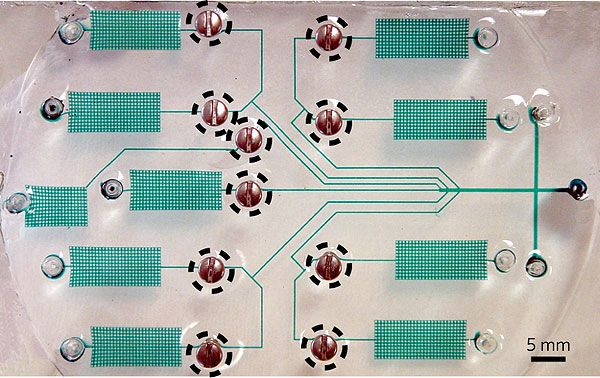
\includegraphics[width=\columnwidth,height=5cm,keepaspectratio]{Torque-immunoassay.jpg}
  \end{center}
  \caption{Coponents of a microfluidic device got increasingly complicated. This device from Ref.\citep{weibel2005torque} performs
  immunoassays - widely used in medical and biological research. The screws circled are manually operated valves. Water with green dye
  shows the channels.}
  \label{fig:immunoassay}
\end{figure}

\begin{itemize}
  \item As these fabrication methods become more widely used the field of microfluidics moved from
  adding components to its analytical
  arsenal, to starting to apply microfluidic systems to resolving problems.
  These systems then found applications in protein cyrstallisation[ref],
  separations coupled with mass spectroscopy[ref], single cell manipulation[ref],
  and synthesis of $^19$F-labelled organic compounds for use in PET
  scans[ref].
  \item A subsection of microfluidics began to emerge around this time too, as
  low reynolds numbers makes multiphase flow manipulation
  relatively easy, the generation and manipulation of droplets[refs] began to be explored.
  These involved dispersing a liquid phase in a continuous
  liquid stream to form a monodisperse emulsion of (often) aqueous droplets in oil. These droplets
  were used to produce polymer particles[ref], in making irregular particles[ref],
  hollow microcapsules[ref], and protein detection in cells\citep{huebner2007quantitative}.
  \item In parallel, another branch of microfluidics was being developed. Its goal was to
  culture cells in a repeatable way. In their normal environment, cells are subject to multiple
  cues that can vary including cytokines and secreted proteins from neighbouring cells, biochemical
  interactions with the extracellular matrix, mechanical stress and direct cell to cell contacts.
  Microfluidics provided cells these cues in a controlled and reproducible fashion that cannot be easily
  replecated with conventional cell culture. The idea at the time was that devices could combine
  cell culture with analytical techniques in order to probe the biochemical processes that
  govern all manner of cell behaviour.
\end{itemize}

\begin{figure}
  \begin{center}
  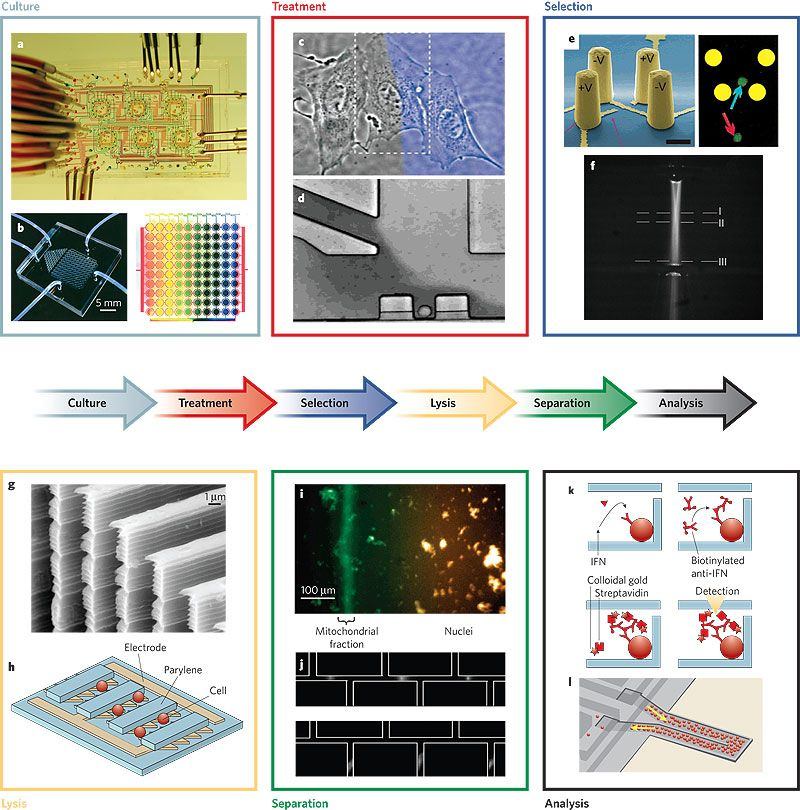
\includegraphics{Microfluidic-Cell-Culture.jpg}
  \end{center}
  \caption{A collection of microfluidic devices that enabled cell based assays from cell culture, to selection and treatment,
  to analysis. \textbf{a}, Six biorexctors are operated in parallel in a single chip to monitor small numbers of cells\citep{balagadde2005long},
  \textbf{b}, Microfluidic cell-culture array with integrated concentration gradient generator (left). Image of concentration
  gradient when blue and yellow dye is used (right)\citep{RN41}. \textbf{c} Two laminar streams exposing two sides of a single cell to different
  conditions\citep{takayama2001laminar}.
  \textbf{d}, Perfusion over a single trapped cell. The perfusion media can be switched in 100 ms\citep{wheeler2003microfluidic}. \textbf{e}, (left) Cell dielectrophoresis
  trap. (right) Fluorescent image of trapped cell indicated by blue arrow\citep{Voldman:2002gf}. \textbf{f}, Fluorescent image of light path at the detection
  zone in a micro flow cytometer\citep{wang2004measurements}. \textbf{g} Scanning electron micrograph of a mechanical lysis device with sharp knife-like protrusions\citep{di2003reagentless}.
  \textbf{h}, Schematic of electrical lysis device with microelectrodes\citep{lee1999micro}. \textbf{i}, Isoelectric focusing of cell organelles\citep{lu2004microfabricated}.
  \textbf{j}, Two-dimensional separation of four model proteins. Isoelectric focusing (top) followed by SDS gel electrophoresis\citep{li2004integration}.
  \textbf{k}, Schematic of immunoassay using microbeads as a solid support\citep{sato2002microchip}. \textbf{l}, Schematic of a hollow cantilever-mased mass sensor
  for analyte detection\citep{burg2003suspended}. Taken from Ref.\citep{el2006cells}}
  \label{fig:CellCulture}
\end{figure}

\begin{itemize}
  \item Microfluidic devices have been used enable cell-based assays from cell culture to biochemical analysis. In
  \fig{fig:CellCulture} images of different devices are shown that convey how complex the devices being produced were becoming,
  depite integration of functionalities proving difficult, these demonstrate the power of miniaturisation and the ingenuity
  being developed in the field.

  \item Late 2000s developments - towards organ on a chip, label free methods of detection needed,
  fluorscence spec, mass spec, flow cytometry, 3D cell culture all becoming more and more advanced [refs]
  \item 2010s to now digital microfluidic platforms becoming successful, micrfluidics now too big for
  broad reviews - many specialised areas that need review of their own - ref ans ummarize some of them.
  \item label free is where µNMR comes in to help - dicussed in microNMR but can breifly mention here
  due to the relevance
  \item This work seeks to combine both fields - bring in from before. This is will be useful due to
  reduced cost involved meaning many experiments can be run in parallel. This technique is also well
  suited to mass limited samples due to its non-destructive nature
\end{itemize}

\begin{figure}
  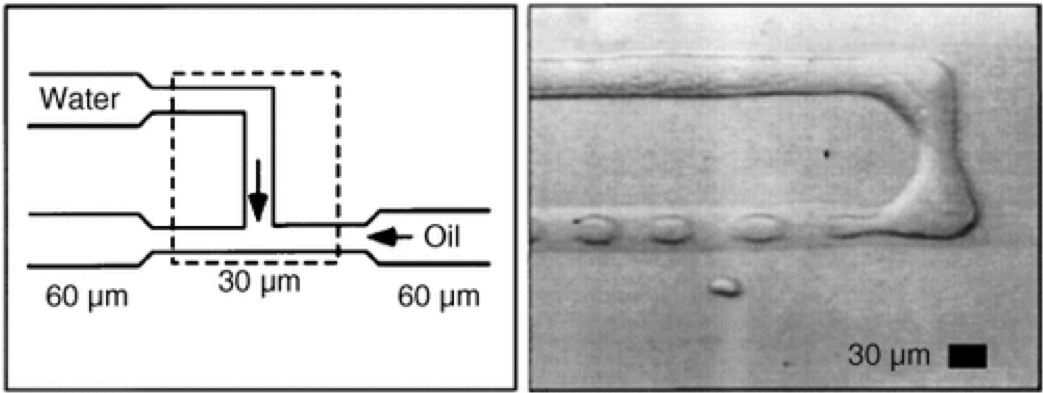
\includegraphics[width=\columnwidth]{Droplets.png}
  \caption{Formation of droplets in a T-Junction of a microfluidic device the continuous hydrocarbon
  phase disperses a water phase. Figure from \citep{RN104}}
  \label{fig:IntroDrops}
\end{figure}


\section{NMR theory}

Nuclear magnetic resonance (NMR) theory can be described using two approaches:
\begin{enumerate}
  \item The classical approach, in which the the nuclei are thought of as small bar magnets which
  rotate in 3D space. Experiments can be described be approxiamating the net magnetisation as a
  vector in 3D space.
  \item The quantum mechanical approach, in which each spin in the system is in a distinct quantised state.
  Operators are used to describe the state of a system as a whole. Experiments are described by propagating
  these operators.
\end{enumerate}

The theory described in this chapter is mainly from \citep{RN135,RN136} and is intended to provide sufficient background
knowledge in order for the reader to understand later chapters.

\subsection{Classical NMR}

\subsubsection{Spin}

Nuclei, often modelled as a clump of neutrons and protons surrounded by electrons at
the centre atoms, have a property reffered to as spin.

In fact, nuclear spin is an intrinsic property of the nucleus and can take half or whole
integer values, including $0$. In this thesis we will be mainly concerned about one spin-
1/2 nucleus, the proton ($\ce{^{1}H}$), with another spin-1/2 nucleus \ce{^{13}C} making
sparse appearences. Just like in this thesis, $\ce{^{13}C}$ only has an $\approx{1}\%$
abundance in nature with the other $\approx{99}\%$ $\ce{^{12}C}$ having a spin-$0$
nucleus.

All spin-1/2 nuclei possess a magnetic dipole moment and behave rather like small bar magnets in that, when placed in an external magnetic field they have a tendency to align
with the field. In NMR this external field is called $B_0$, and is orientated along the
$z$-axis.

\subsubsection{Population}\label{Population}

In a magnetic field a spin-1/2 nucles has two energy levels with a separation that is proportional to the strength of the magentic field a schematic is show in \fig{fig:EnergySplit}. We label these levels $\alpha$ and $\beta$.

\begin{figure}
  \begin{center}
  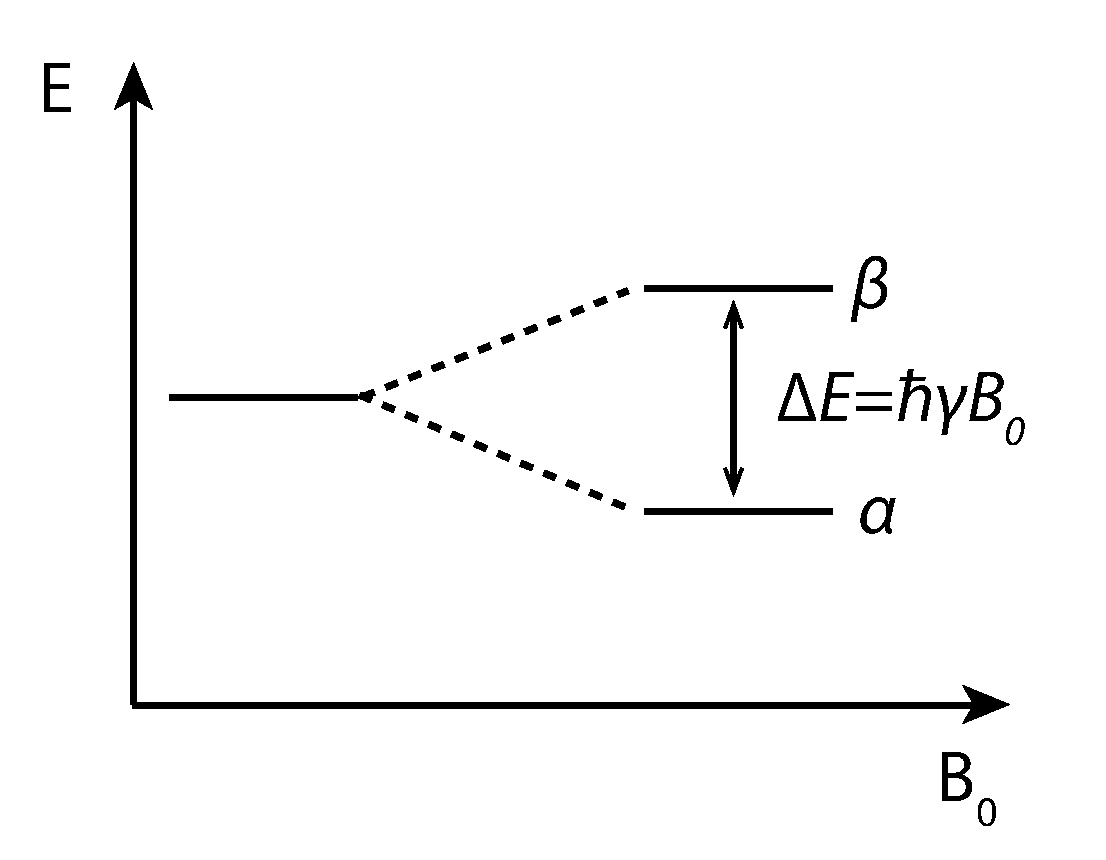
\includegraphics[width=\textwidth,height=5cm,keepaspectratio]{EigenStateLevel.pdf}
  \end{center}
  \caption{Energy level and $\Delta~E$ of the two energy levels for a spin-1/2 nucleus}
  \label{fig:EnergySplit}
\end{figure}

When measuring a group of spins each spin can exist in either the $\alpha$ or $\beta$ state and overall the spins have a slight preference for the lower energy state, $\alpha$. This preference can be quantified by calculating the difference in populations ($P$) which at thermal equilibrium is governed by the Boltzmann distribution:
\begin{equation}\label{eqn:Boltzmann}
  \frac{P_{\beta}}{P_{\alpha}} = \text{exp}\{\frac{-\Delta{E}}{k_B T}\}
\end{equation}

where $P_{\beta}/P_{\alpha}$ is the population ratio between the states, $k_B$ is Boltzmann constant, and $T$ is the temperature. The polarisation, $p$, of a system of
spin-1/2 nuclei is
\begin{equation}
  p = \frac{P_\alpha - P_\beta}{P_\alpha + P_\beta}
\end{equation}

For a system in an NMR experiment which typically operates at 298$K$ and
a field of 14.1 T the polarisation level is circa $10^5$ meaning That the spins are aligned weakly in the same direction as the magnetic field. It is this small polarisation that gives rise to the NMR signal and why NMR is famed for sensitivity
issues. One possible solution to this will be described in a later chapter.

\subsubsection{Nuclear spin precession}

When placed in a magnetic field, the nuclei will precess around the axis of the field at a rate known as the larmour frequency defined as:
\begin{equation}\label{eqn:larmour}
  \omega_j^0 = -\gamma_jB_0
\end{equation}

where $\gamma_j$ is the gyromagnetic ratio for a nucleus, $j$. The gyromagnetic ratio is
typically $10$s of MHz T$^{-1}$ that give larmour frequencies in the $100$s of MHz in an NMR
experiment.

\subsubsection{Magnetisation as a vector}

The net magnetic moment of a spin ensemble can be modelled by a 3D vector that can rotates in space. The essence of this is shown in \fig{fig:VectorFig}. Magnetisation is intially taken to be orientated along the $z$-axis, this is called longitudinal magnetisation. It is then rotated into the $xy$-plane which is called transverse
magnetisation that then precesses about the $z$-axis.

\begin{figure}
  \begin{center}
  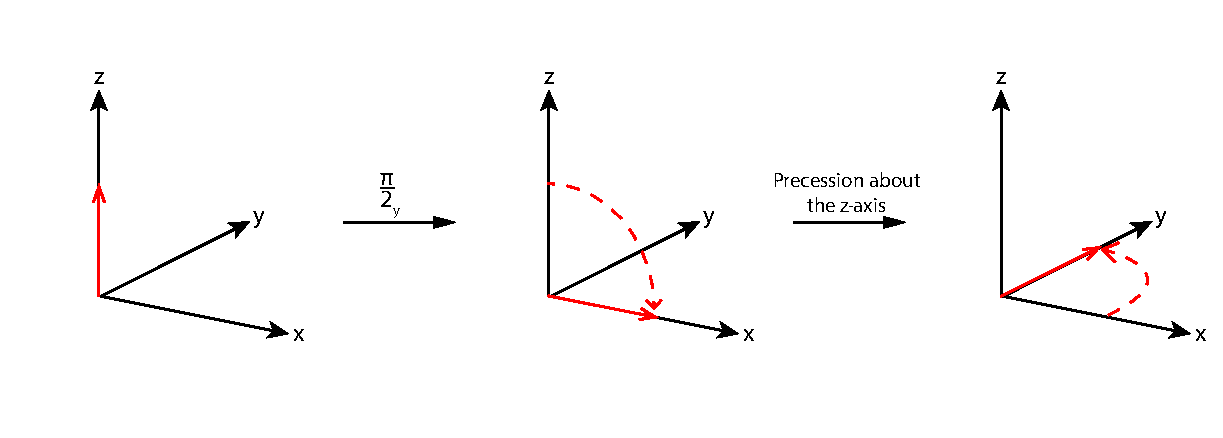
\includegraphics[width=\textwidth]{VectorFig.pdf}
  \end{center}
  \caption{Magnetisation shown as a vector in red, at equilibrium, is orientated on the $z$-axis. A $pi$/2
  pulse rotates the vector to the $xy$-plane where it begins to precess around the $z$-axis.}
  \label{fig:VectorFig}
\end{figure}

How this vector changes in a magnetic field is described using the Bloch equations\citep{Bloch:1946hk}. These are a group of differential equations that
describe how the magnetisation vector components evolves in time in the
presence of orthogonal magnetic fields.
\begin{align}\label{eqn:Bloch}
  \frac{dM_x(t)}{dt}\quad=\quad\gamma(M_y(t)B_z(t)-M_z(t)B_y(t))\\
  \frac{dM_y(t)}{dt}\quad=\quad\gamma(M_z(t)B_x(t)-M_x(t)B_z(t))\\
  \frac{dM_x(t)}{dt}\quad=\quad\gamma(M_x(t)B_y(t)-M_y(t)B_x(t))
\end{align}
where $M_a$ is the magnetisation vector component along the $a$-axis, $B_a$ is the
magnetic field along the $a$-axis, and $\gamma$ is the gyromagnetic ratio as described before.

In the case of processing magnetisation around the $z$-axis, here denoted $B_0$, the
Bloch equations can be written as
\begin{align}
  \frac{dM_x(t)}{dt}\quad=&\quad\gamma~B_0M_y(t)\\
  \frac{dM_x(t)}{dt}\quad=&\quad-\gamma~B_0M_x(t)\\
  \frac{dM_x(t)}{dt}\quad=&\quad0
\end{align}
these have the solutiion
\begin{align}
  \frac{dM_x(t)}{dt}\quad=&\quad\cos(\omega^0t)M_x(0) + \sin(\omega_0t)M_y(0)\\
  \frac{dM_x(t)}{dt}\quad=&\quad\cos(\omega^0t)M_y(0) + \sin(\omega_0t)M_x(0)\\
  \frac{dM_x(t)}{dt}\quad=&\quad0
\end{align}
where $\omega^0$ is the larmour frequency from \eqn{eqn:larmour}.

\subsubsection{Pulses and rotating frame}

\subparagraph{Rotating frame}

The field, $B_0$, of a regular NMR experiment is many Tesla, giving precession
frequencies of hundreds of megahertz. These frequencies correspond to radio frequencies in the electromagnetic spectrum. Considering these precessing spins
it can be useful to change from a static frame to a rotating frame of reference.

The general case is when the rotating frame is at frequency $\omega_{rot}$, in this
frame, the larmour frequency will appear to be ($\omega - \omega_{\text{rot}})$. This is called the offset,$\Omega$ and is given by:
\begin{equation}
  \Omega = \omega -\omega_{\text{rot}}
\end{equation}

It follows from this, that if the apparent larmour frequency in the rotating frame is different from that in the static frame, it must also be the case that the apparent magnetic field in the rotating frame must be different from the applied
field. We can use \eqn{eqn:larmour} to compute the apparent magnetic field, $B^{\text{red}}_0$:
\begin{align}\label{eqn:redB}
  \Omega =& -\gamma~B^{\text{red}}_0\\
\text{hence}\quad~B^{\text{red}}_0 =& \frac{\Omega}{\gamma}
\end{align}
this apparent magnetic field in the rotating frame is called the reduced field.

\begin{figure}
  \begin{center}
  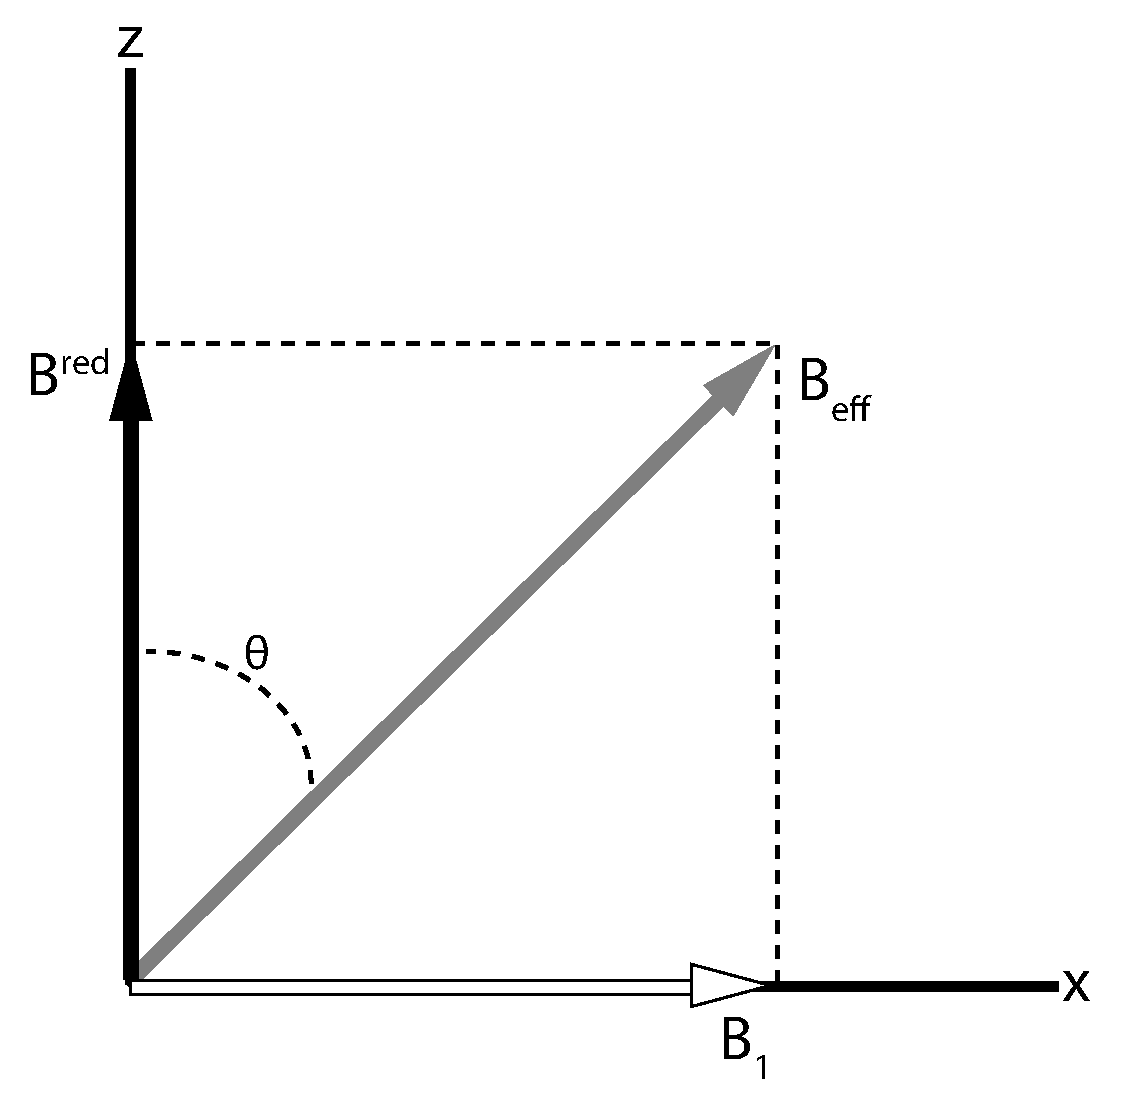
\includegraphics[width=\textwidth, height=7cm, keepaspectratio]{B1Bred.pdf}
  \end{center}
  \caption{In the rotating frame the effective field, $B_{\text{eff}}$, is the vector sum of the reduced field,
  $B_{\text{red}}$ and the $B_1$ field. $\theta$ is the tilt angle defined between $B_{\text{red}}$ and $B_{\text{eff}}$}
  \label{fig:BMag}
\end{figure}


\subparagraph{Pulses}

In NMR experiments pulses are used to manipulate magnetisation in order to obtain a signal. A pulse can be
thought of as a magnetic field oscillating at the frequency of the rotating frame
applied in the $xy$-plane in order to induce procession of the magnetisation. This magnetic field is labelled $B_1$ and is much smaller in amplitude than $B_0$, the actual applied field.

\begin{figure}
  \begin{center}
  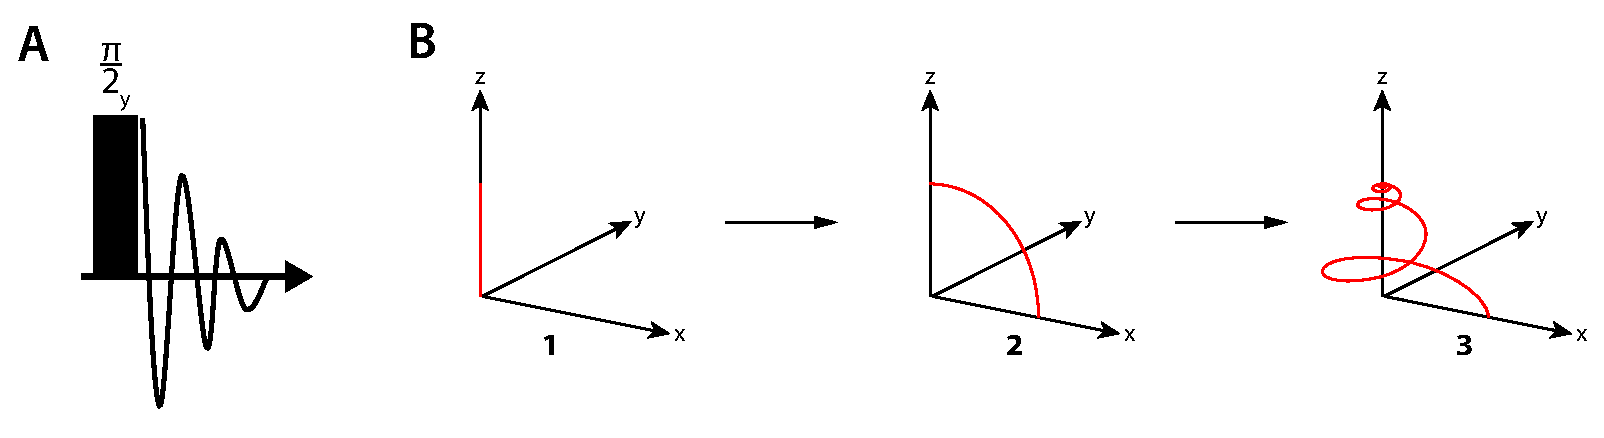
\includegraphics[width=\textwidth]{SpinRelaxation.pdf}
  \end{center}
  \caption{A) A graphical representation used to describe a pulse sequence, the width and height of the block
  refer to the power and duration of pulse respectively, the line represents the acquisition of signal. B)(1) The
  magnetisation lies in equilibrium along the $z$-axis. (2)  The $\pi/2_y$ pulse rotates the magnetisation around the $y$-axis. (3) The magnetisation precesses in the $xy$-plane around the $z$-axis and returns to thermal equilibrium}
  \label{fig:Pulse}
\end{figure}

In the static frame, the magnetisation is processing around $B_0$ at the larmour frequncy, so a relatively weak $B_1$ applied along the $y$-axis, for example, would do little to peturb it, given the effective magnetic field, $B^{\text{eff}}_0$, is calculated by:
\begin{equation}
  B^{\text{eff}}_0 = \sqrt{(B_1)^2+(B_0)^2}
\end{equation}
the much larger $B_0$ dominates here, however, if we apply the $B_1$ in the rotating
frame this becomes
\begin{equation}
  B^{\text{eff}}_0 = \sqrt{(B_1)^2+(B^{\text{red}}_0)^2}
\end{equation}
and using \eqn{eqn:redB} as $\omega_{\text{rot}}\rightarrow\omega$, $\Omega\rightarrow0$ and $B^{red}_0\rightarrow0$ so by making the offset small, or zero, the effective field
then lies close to the $xy$-plane and so the magnetisation will be rotated down
from $z$ which is what we'd like to acheive for our experiments.

The key, is that although $B_0$ is much larger than $B_1$, we can still affect magnetisation using $B_1$ by making it oscillate close to the larmour frequency
this is the phenomena of resonance. The angle between $B^{\text{red}}_0$ and $B^{\text{eff}}$ is
called the tilt angle, $\theta$. It can be seen from \fig{fig:BMag} that:
\begin{equation}
\sin(\theta) = \frac{B_1}{B_{\text{eff}}}\qquad\cos(\theta) = \frac{B^{red}_0}{B_{\text{eff}}}\qquad\tan(\theta) = \frac{B_1}{B^{\text{red}}_0}
\end{equation}

These radio frequency (rf) pulses are useful because they can be used to address spins at a specific larmour
frequncy. By applying an rf pulse on resonance with $\ce{^1H}$ we can manipulate the magnetisation of the nuclei whislt not affecting other spins (e.g. $\ce{^13C}$) contained in the sample.

\subsubsection{Fourier Transform NMR}

In this section we will examine how we can produce an NMR spectrum from the magnetisation of a sample
using the rf pulses we introduced.

In NMR we use a pulse sequence to describe the intensity and duration of pulses used in an
experiment, shown in \fig{fig:Pulse}. The rf pulse, $B_1$, is a $\pi/2$ pulse in the $y$-axis, followed by a signal
acquisition. This pulse tips the magnetisation into the $xy$-plane, and if the pulse length is much less than the
precession period (we will assume so), the spins begin to precess freely around the $z$-axis at the larmour
frequency, $\omega_0$, until they return to the $z$-axis through a process described in \ref{Relaxation}.

In a usual NMR experiment the signal is inductally detected. The oscillation of the spins in the sample induces
a current in the pick-up coils around the sample, which is detected, amplified and transformed into a spectrum.
The resulting free induction decay (FID) is typically an exponentionally decaying sinusoidal function. The signal
produced from this can be written as:
\begin{align}\label{eqn:signal}
  S(t) =& \sum_l s_l(t) \\
  s_l(t) =& a_l\text{exp}\{-(i\omega_l+\lambda_l)t\} = a_l(\cos(\omega_lt) + i\sin(\omega_0t))\text{exp}\{-\lambda_l~t\}
\end{align}
where $S(t)$ is the total signal from from the sample and $s_l$ are the individual spins. Each spin has an amplitude, $a_l$, and an associated decay constant, $\lambda_l$. The nature of which will be discussed in \ref{Relaxation} section. Exponential to trigometric function conversion
is done according to Euler's formula: $\text{exp}\{ix\} = \cos(x) + i\sin(x)$.

$S(t)$ is easy to evaluate and interpret if it originates from one spin or a group of spins precessing
at precisely the same frequency, however, if there are more spins in the sample processing at different frequencies
the FID becomes extremely hard to interpret on its own.

We can clear this picture up however by employing a Fourier transform. This comverts the time-domain data
into the frequncy-domain, such that the total signal in the frequency domain, $S(\omega)$ is the sum of all individual spin signals in the frequency, $S_l(\omega)$:
\begin{equation}
  S(\omega) = \sum_l S_l(\omega)
\end{equation}
This allows us to clearly see which resonances are possessed by our spins in the sample. To
perform a Fourier transform we must do the following:
\begin{equation}
  S_l(\omega) = \int_{0}^{\infty}s_l(t)\text{exp}\{-i\omega t\}dt
\end{equation}
and using \eqn{eqn:signal} can be rewritten:
\begin{equation}
  S_l(\omega) = a_l\int_{0}^{\infty}\text{exp}\{(-i(\omega+\omega_l)+\lambda_l t\}dt
\end{equation}
sometimes written more concisely as:
\begin{equation}
  S(\omega) = \mathcal{F}\{S(t)\}(\omega)
\end{equation}
where $S(t)$ is the signal for the time domain (FID) and $S(\omega)$ is the signal in the frequency domain.

The Fourier transform of our general case is:
\begin{equation}
  \mathcal{F}\{S(t)\}(\omega) = a_l\frac{1}{\lambda_l + i(\omega - \omega_l)}
\end{equation}
which is Lorentzian function centered at $\omega_l$ with peak width parameter $\lambda_l$.

The NMR signal represented in the frequency domain is a spectrum. It is usually many peaks
indicating different resonance frequencies of spins in the sample. In the next
section we will discuss chemical shift and J-coupling. Two additional effects that when combined
with larmour frequencies already discussed forms the NMR spectrum as we know it.

\subsubsection{Chemical Shift and J-coupling}

In a molecule, nuclei are surrounded by clouds of electrons which can shield, or de-sheild, it
from the effects of the external field $B_0$.

The chemical shielding factor, $sigma$, shifts the resonance frequency of the nuclear spin. We
can now include it in \eqn{eqn:larmour}:
\begin{equation}
  \omega_j^0 = -\gamma_jB_0(1-\sigma)
\end{equation}
this chemical shielding is specific to each nucleus in the molecule. It is possible
for two or more nuclei to share the same factor. We refer to these as being chemically equivalent.

The shielding is often around $10^-6$ for $\ce{^1H}$. When plotting and examining spectra
it is would not be useful to use absolute frequecies, as discussed they are regualarly in the hundreds of MHz,
whereas the differences in peaks might only be kHz or less. To combat this we use a relative frequency scale
called chemical shift, $\delta$, it is defined as:
\begin{equation}
  \delta = \frac{\omega_j-\omega^\text{ref}_j}{\omega^\text{ref}_j}
\end{equation}
where $\omega_j$ is the precession frequency of the nucleus of interest, and $\omega^\text{ref}_j$ is the precession
frequency of a reference nuclei. $\delta$ is a dimentionless number, unaffected by magnetic field strength, it often
small compared to the size of the field and is reported in parts per million (ppm).

In addition to the external $B_0$ field, the nuclear spins are also affected by the magnetic fields generated
by neighboring spins. These magnetic fields are mediated by the electrons in the chemical bonds. This is refered to as
spin-spin couling or $J$-coupling and gives rise to peak splittings in spectra. These splittings, and therefore the values of $J$-couplings, range from a few Hz to a thousand Hz typically. It is an important factor and is icorperated
in the quatum description on NMR in \ref{Hamiltonian}.

Both of these, $\sigma$ and $J$-couplings, are tensors this means they depend on the orientation of the molecule
and the spin with respect to the magetic field. In liquids, however, tumble rapidly compared to the timescale
of an NMR experiment. This averages the interactions resulting in a scalar quantity for each.

There are additional effects the nuclear spins experience, for example, dipole-dipole coupling which
is a through space spin-spin coupling, and quadrapole coupling where there are spins with >1/2 values
however, these are not relevant to this work.

\subsubsection{Relaxation}\label{Relaxation}

The last part needed to complete our classical understanding of NMR is relaxation. Relaxation is the process
of the spin returning to the thermal equilibrum. The thermal equilibrium of spin-1/2 nuclei in a
magnetic field is the bulk magnetisation vector pointing in the direction of the $B_0$ field.

In this system there are two forms of relaxation, $T_1$ and $T_2$. $T_1$ is the longitudal relaxation time
constant and $T_2$ is the transverse relaxation time constant the difference between them is shown in \fig{fig:t1t2}.
$T_1$ is the rate constant that governs the return of magnetisation to the $z$-axis from the $xy$-plane. $T_2$ on
the other hand is the time constant that governs the return of magnetisation to equilibrium in the $xy$-plane.
It is more accurate to say that $T_1$ is the relaxation rate constant for populations, and $T_2$ is the relaxation
rate constant coherences, in the density operator (discussed in \ref{Quantum}). But this is incompatible
with the classical description of NMR.

We can now complete the Bloch equations from \eqn{eqn:Bloch}:
\begin{align}
  \frac{dM_x(t)}{dt}\quad=&\quad\gamma(M_y(t)B_z(t)-M_z(t)B_y(t)) - \frac{M_x(t)}{T_2}\\
  \frac{dM_y(t)}{dt}\quad=&\quad\gamma(M_z(t)B_x(t)-M_x(t)B_z(t)) - \frac{M_y(t)}{T_2}\\
  \frac{dM_zt)}{dt}\quad=&\quad\gamma(M_x(t)B_y(t)-M_y(t)B_x(t)) - \frac{M_z(t)-M_0}{T_1}
\end{align}
in order to derive $M_{xy}$ we assume the following:
\begin{equation}
  M_{xy} = M_x + iM_y\qquad\text{and} B_{xy} = B_x + iB_y
\end{equation}
After some algebra we obtain:
\begin{align}
  \frac{dM_xy(t)}{dt}\quad=&\quad-i\gamma(M_{xy}(t)B_z(t)-M_z(t)B_{xy}(t)) - \frac{M_{xy}(t)}{T_2}\\
  \frac{dM_y(t)}{dt}\quad=&\quad~i~\frac{\gamma}{2}(M_{xy}(t)\overline{B_{xy}}(t)-\overline{M_{xy}}(t)B_z(t)) - \frac{M_y(t)}{T_2}\\
\end{align}
where $\overline{M_{xy}} = M_x - iM_y\qquad\text{and} \overline{B_{xy}} = B_x - iB_y$
solving these gives:
\begin{align}
  M_z(t) =& M_{z,\text{eq}} - (M_{z,\text{eq}}-M_z(0))\text{exp}\{\frac{-t}{T_1}\}\\
  M_{xy}(t) =& M_{xy}(0)\text{exp}\{\frac{-t}{T_2}\}
\end{align}

\begin{figure}
  \center{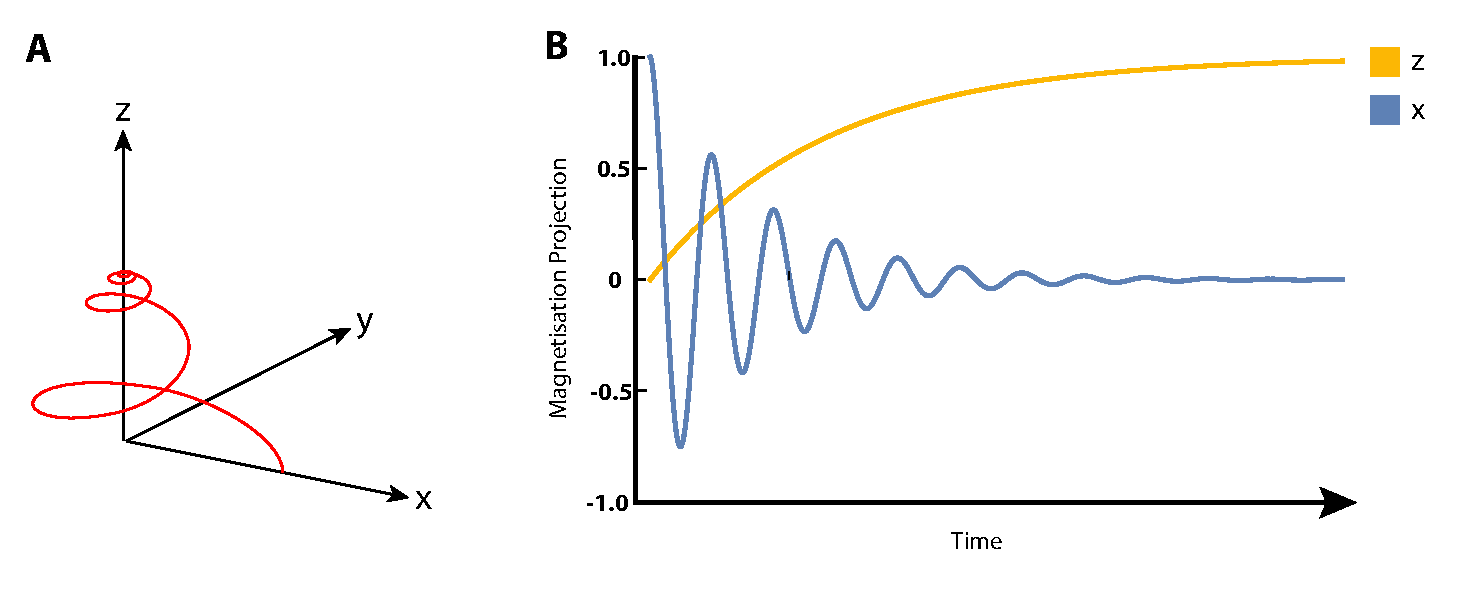
\includegraphics[width=\textwidth]{T1T2.pdf}}
  \caption{A) a magnetisation vector precesses in the $xy$-plane, eventually returning to equilibrium.
  B) A plot of the magnetisation along $z$-axis (yellow) and the $x$-axis (blue) during the relaxation.}
  \label{fig:t1t2}
\end{figure}

Relaxation occurs when the spins exchange energy with their surroundings. They do
this when local magnetic fields, usually caused by the motion of surrounding molecules, oscillate
near the larmour frequency of the relaxing spin. These oscillating fields can be thought of
as local RF pulses we discussed earlier, the key difference is that they only affect a few spins
and not the sample as a whole. Essentially relaxation is an energy exchange between the
spins and the molecules surrounding them. This is the origin of the original name for longitudal
relaxation - spin-lattice relaxation.



\subsection{Quantum description of NMR}\label{Quantum}

In this chapter, I will introduce the the quantum description of NMR. Including how
we use operators and superoperators to understand how states change under different conditons and how the energies of the system can be extracted.

\subsubsection{Nuclear Spin}

Nuclear spin can be treated as a type of angular momentum. Spin angular momentum can be characterized by its total
angular momentum, and the angular momentum with respect to a reference axis (usually z).  Denoted by $\hat{I}$
it is comprised of a magnitude, $\lvert\hat{I}\rvert$, and a direction, $m_I$.
The magnitude is given by
\begin{equation}
  \lvert\hat{I}\rvert = \hbar\sqrt{I(I+1)}
\end{equation}
where $\hbar$ is the reduced Planck constant and $I = 0,\frac{1}{2},1,\dots$. The projection of $\hat{I}$ in
the $z$ direction, $\hat{I}_{z}$, is given by
\begin{equation}
  \hat{I}_{z} = m_I\hbar
\end{equation}
$m_{I}$ can take integer values from $-I$ to $+I$ shown in \fig{fig:Projection}

For the commonly occuring case of a spin-1/2 nucleus, $I=1/2$ and $m_I = ±1/2$ and if we were to measure $\hat{I}_z$ we would get a value of  with an associated probability depending which state the system is in. Indicating the possible measurement outcomes for $\hat{I}_z$ are $±\frac{\hbar}{2}$.

\begin{figure}
  \begin{center}
  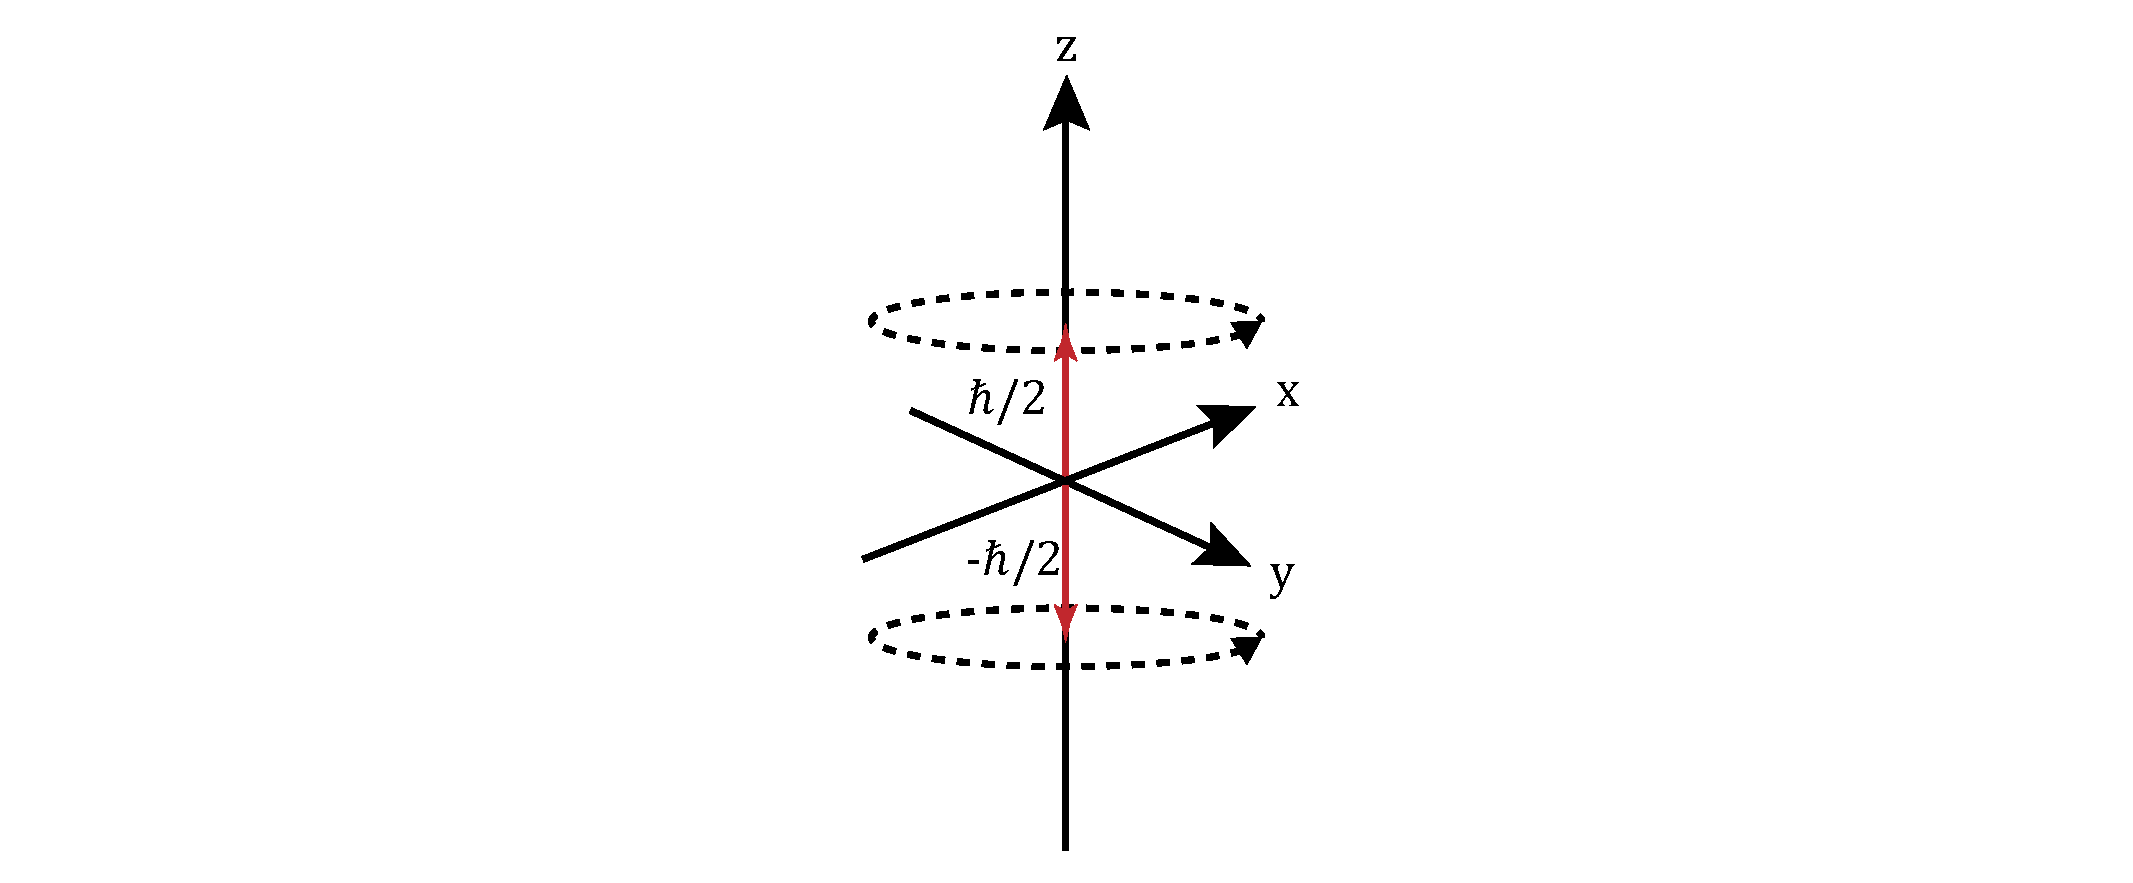
\includegraphics[width=\columnwidth,height=5cm,keepaspectratio]{StateProjection.pdf}
  \end{center}
  \caption{The projection of two states in a spin 1/2 nucleus (red arrow) with the magnitudes indicated (black arrow)}
  \label{fig:Projection}
\end{figure}

\subsubsection{Spin States}\label{SpinStates}

If a spin-1/2 nucleus is placed in a magnetic field (taken to be oriented along $z$) it can be represented using two basis states.
State one has $I = 1/2$, $m_I = 1/2$ and State two has $I = 1/2$, $m_I = -1/2$. We denote these as $\ket{I,m_I}$\citep{dirac_1939}, for simplicity we omit the $I$ and are left with
$\ket{m_I}$. For the special case of a spin-1/2 the two states are known as zeeman states denoted by $\ket{\alpha}$ and $\ket{\beta}$. Where the $\ket{\alpha}$ state has angular momentum +1/2 and $\ket{\beta}$ has -1/2.

The zeeman states take the following form:

\begin{equation}
  \ket{\alpha} = \begin{pmatrix}
    1\\
    0
\end{pmatrix}
 \ket{\beta} = \begin{pmatrix}
   0\\
   1
\end{pmatrix}
\end{equation}

bras are also defined by taking the conjugate transpose of the ket, $\ket{\alpha}^{\dagger} =
\bra{\alpha}$ such that
\begin{equation}
  \bra{\alpha} = \begin{pmatrix}
    1 & 0
\end{pmatrix}
  \bra{\beta} = \begin{pmatrix}
  1 & 0
\end{pmatrix}
\end{equation}

The state, $\ket{\psi}$, of a two level system can now be completely decribed in this basis
as the linear combination of the basis states:
\begin{equation}\label{eqn:zeeman}
  \ket{\psi} = c_1\ket{\alpha} + c_2\ket{\beta} = \begin{pmatrix}
    c_1\\
    c_2
\end{pmatrix}
\end{equation}
\begin{equation}
  \bra{\psi} = c_1^*\bra{\alpha} + c_2^*\ket{\beta} = \begin{pmatrix}
    c_1^* & c_2^*
\end{pmatrix}
\end{equation}

These are normalised such that $c_1c_1^* + c_2c_2^* = 1$.

To complete the picture the sates must me orthonormal. Orthonormality between states exists if
if the inner product of the basis states $\ket{r_i} ~\text{and}~ \ket{r_j}$ satisifies the following conditions:

\begin{equation}
  \langle r_i\vert r_j\rangle = \delta_{ij}
\end{equation}

where the Kronecker delta is:
\begin{equation}
  \delta_{ij} = \begin{cases}
    0 & ~\text{if}~ i \ne j\\
    1 & ~\text{if}~ i = j
                \end{cases}
\end{equation}

where $\langle r_i\vert r_j\rangle = \delta_{ij}$ denotes taking the dot product between the two
vectors $\ket{r_i}$ and $\ket{r_j}$.

The basis states help to quantify the component of a state vector along that state. Take our example from \eqn{eqn:zeeman}, we can construct inner products of the overall state, $\ket{\psi}$ with $\ket{\alpha}$ and $\ket{\beta}$ to determine component of the basis states.
\begin{equation}
  \langle\alpha\vert\psi\rangle = c_1 \quad \langle\beta\vert\psi\rangle = c_2
\end{equation}

The outer product of the basis state, $\ket{r_n}$, for an N-spin system must satisfy:
\begin{equation}
  \sum_{n=1}^{N} \ket{r_n}\bra{r_n} = \mathbb{1}
\end{equation}

where $\mathbb{1}$ is an N by N identity matrix.

When a second spin is introduced, the Hilbert space is extended to accommodate additional spin
states by taking the tensor product of the basis states


\begin{align}\label{eqn:2spinstates}
\ket{\alpha_{1}\alpha_{2}} = \ket{\alpha_1} \otimes \ket{\alpha_2} = \begin{pmatrix}
  1\\
  0\\
  0\\
  0
\end{pmatrix} &
\ket{\alpha_{1}\beta_{2}} = \ket{\alpha_1} \otimes \ket{\beta_2} = \begin{pmatrix}
  0\\
  1\\
  0\\
  0
\end{pmatrix}\\
\ket{\beta_{1}\alpha_{2}} = \ket{\beta_1} \otimes \ket{\alpha_2} = \begin{pmatrix}
  0\\
  0\\
  1\\
  0
\end{pmatrix} &
\ket{\beta_{1}\beta_{2}} = \ket{\beta_1} \otimes \ket{\beta_2} = \begin{pmatrix}
  0\\
  0\\
  0\\
  1
\end{pmatrix}
\end{align}
The subscripts indicate which spin we are reffering to, e.g. $\ket{\beta_1\alpha_2}$ means that
spin 1 is in the $\beta$ state and spin 2 is in the $\alpha$ state.

\subsubsection{Operators}

Operators act on states. To explain this, let's consider a generic operator $\hat{B}$ with eigenstates $\ket{\alpha}$ and $\ket{beta}$. When a state is acted upon by an operator it is denoted by:
\begin{equation}
  \hat{B}\ket{\alpha} = b\ket{\alpha}
\end{equation}

the same state is returned, multiplied by some scalar $b$, that is an eigenvalue of $\ket{\alpha}$
in the operator basis B.

The expectation value of an operator can be found by:
\begin{equation}\label{eqn:expectation}
  \langle\hat{B}\rangle = \langle\alpha\vert\hat{B}\vert\alpha\rangle = b\langle\alpha\vert\alpha\rangle = b
\end{equation}

this returns the eigenvalue.

In NMR we use three operators to determine the projection of angular momentum along a specific axis, $\hat{I}_x$, $\hat{I}_y$, and $\hat{I}_z$. These are defined by the Pauli matrices multiplied by $\frac{\hbar}{2}$.

\begin{equation}
  \hat{I}_x=\frac{\hbar}{2}\begin{pmatrix}
    0 & 1\\
    1 & 0
\end{pmatrix}\quad
\hat{I}_y=\frac{\hbar}{2i}\begin{pmatrix}
  0 & 1\\
  -1 & 0
\end{pmatrix}\quad
\hat{I}_z=\frac{\hbar}{2}\begin{pmatrix}
  1 & 0\\
  0 & 1
\end{pmatrix}
\end{equation}

as an example, let's take the example from before of a spin-1/2 particle in a magnetic field
and see what happens if we were to project the $\ket{\alpha}$ state along the z-axis.
\begin{equation}\label{eqn:operators}
  \hat{I}_z\ket{\alpha} = \frac{\hbar}{2}\begin{pmatrix}
    0 & 1\\
    1 & 0
\end{pmatrix}
\begin{pmatrix}
  1\\
  0
\end{pmatrix} = \frac{\hbar}{2}\begin{pmatrix}
  1\\
  0
\end{pmatrix} = \frac{\hbar}{2}\ket{\alpha}
\end{equation}
We find that $\frac{\hbar}{2}$ is the eigenvalue of $\ket{\alpha}$ for the operator $\hat{I}_z$. For ease of handling in the following examples we will take $\hbar$ = 1.

We will now examine three more operators and explore how they act on states. They are the total square angular momentum, $\hat{I}^2$ and the two shift operators $\hat{I}^+$ and $\hat{I}^-$ defined as the following:

\begin{align}
  \hat{I}^2 =& \hat{I}_x^2 + \hat{I}_y^2 + \hat{I}_z^2\\
  \hat{I}^+ =& \hat{I}_x + i\hat{I}_y\\
  \hat{I}^- =& \hat{I}_x - i\hat{I}_y
\end{align}
They act on states according to:
\begin{align}
  \hat{I}^2\ket{I,m_I} =& I(I+1)\ket{I, m_I}\\
  \hat{I}^+\ket{I,m_I} =& \sqrt{(I(I+1)-m_I(m_I+1))}\ket{I,m_{I+1}}\\
  \hat{I}^-\ket{I,m_I} =& \sqrt{(I(I+1)-m_I(m_I-1))}\ket{I,m_{I-1}}
\end{align}
Using a spin-1/2 particle in a magnetic field as an example we'll let these operators act on the $\ket{\alpha}$ state
\begin{align}
  \hat{I}^2\ket{\alpha} =& \frac{3}{4}\ket{\alpha}\\
  \hat{I}^+\ket{\alpha} =& 0\\
  \hat{I}^-\ket{\alpha} =& \ket{\beta}\\
  \hat{I}^+\ket{\beta} =& \ket{\alpha}\\
  \hat{I}^-\ket{\beta} =& 0
\end{align}
As the '+' and '-' denote raising or lowering $m_I$ by 1


We can see if two operators commute by using the commutator which is defined as:
\begin{equation}
  [\hat{A},\hat{B}] = \hat{A}\hat{B} - \hat{B}\hat{A}
\end{equation}

If $[\hat{A},\hat{B}] = 0$ the operators are said to commute. The $\hat{I}_z$, $\hat{I}_z$ and $\hat{I}_z$
have cyclic commutation rules:
\begin{align}\label{eqn:commutator}
  [\hat{I}_x,\hat{I}_y] = i\hat{I}_z\\
  [\hat{I}_y,\hat{I}_z] = i\hat{I}_x\\
  [\hat{I}_x,\hat{I}_z] = i\hat{I}_y
\end{align}

These relationships are important in NMR as they help govern the rules for the rotations of spins.

\subsubsection{Superoperators}

Like states, that can be transformed by operators, we can define objects that act in a similar manner on operators. These objects are called superoperators.

To start, let's take a simple commutation superoperator, $\hat{\hat{A}}$, defined as:
\begin{equation}
  \hat{\hat{A}}\hat{B} = [\hat{A},\hat{B}] = \hat{A}\hat{B} - \hat{B}\hat{A}
\end{equation}
Applying it to operator $\hat{B}$ results in the commutation of $\hat{A}$ and $\hat{B}$

In NMR, three rotational superoperators can be defined using the commutation superoperators from \eqn{eqn:operators}:
\begin{equation}
 \hat{\hat{R}}_x(\theta) = \text{exp}\{-i\hat{\hat{I}}_x\theta\}\quad\hat{\hat{R}}_y(\theta) = \text{exp}\{-i\hat{\hat{I}}_y\theta\}\quad\hat{\hat{R}}_z(\theta) = \text{exp}\{-i\hat{\hat{I}}_z\theta\}
\end{equation}

These are applied to to the angular momentum operators using the sandwich formula:
\begin{equation}
  \hat{\hat{R}}_x(\theta)\hat{I}_z = \text{exp}\{-i\hat{\hat{I}}_x\theta\}\hat{I}_z\text{exp}\{+i\hat{\hat{I}}_x\theta\}
\end{equation}

The result of this is a rotation of $\hat{I}_z$ around the $x$-axis by an angle $\theta$:
\begin{equation}
  \hat{\hat{R}}_x(\theta)\hat{I}_z = \cos{\theta}\hat{I}_z - \sin{\theta}\hat{I}_y
\end{equation}

The rotational direction (sign of the $\sin{\theta}$ term) is determined by the right hand co-ordinate system defined in \eqn{eqn:commutator}.

We will now discuss how these are used in describing the spin dynamics of a spin system.

\subsubsection{Density Operator}

The density operator gives us information on the state of groups of spins in a spin system.

Let's go back once again to a spin-1/2 particle in a magnetic field. Where $\ket{\psi}$ is some superposition state in the two level system such that:
\begin{align}
\ket{\psi} =& \begin{pmatrix}
    c_1\\
    c_2
\end{pmatrix} = c_1\ket{\alpha} + c_2\ket{\beta}\\
\bra{\psi} =& \begin{pmatrix}
  c_1^* & c_2^*
\end{pmatrix} = c_1^*\bra{\alpha} + c_2^*\bra{\beta}
\end{align}

The density operator has the form:
\begin{equation}
  \hat\rho = \overline{\ket{\psi}\bra{\psi}} = \begin{pmatrix}
    c_1c_1^* & c_1c_2^*\\
    c_2c_1^* & c_2c_2^*
\end{pmatrix}
\end{equation}

If the number of spins is increased, the denstiy operator's form does not change instead it provides
an average fo the entire group of spin states. The population of a given state is given by the expectation value of the density operator as in \eqn{eqn:expectation}. If we would like to know
the population of state $\ket{\alpha}$ we would perform the following:
\begin{equation}
  \langle\alpha\vert\hat\rho\vert\alpha\rangle = \langle\alpha\vert\psi\rangle \langle\alpha\vert\psi\rangle = c_1^*c_1
\end{equation}

The diagonal elements of $\hat\rho$ are state populations or the probabilities of being in a certain state.

The off-diagonal elements are coherences between states. These coherences are complex numbers and two coherences between the same pair of states are complex cojugates of each other. e.g.:
\begin{equation}
  \langle\alpha\vert\hat\rho\vert\beta\rangle = (\langle\beta\vert\hat\rho\vert\alpha\rangle)^* = c_1c_2^* = (c_1^*c_2)^*
\end{equation}
The coherence order between two states in a magnetic field is defined as the difference in angular
momentum projection along the $z$ axis. In our two spin this would be(with $\hbar = 1$):
\begin{align}
  \hat{I}_z\ket{\beta} = m_\alpha = +\frac{1}{2}\ket{\alpha}\\
  \hat{I}_z\ket{\beta} = m_\beta = -\frac{1}{2}\ket{\beta}
\end{align}
We can use these results to calculate the coherence order of the coherence $\langle\alpha\vert\hat\rho\vert\beta\rangle$:
\begin{equation}
 m_\alpha - m_\beta = +1
\end{equation}
and conversely the coherence order of $\langle\beta\vert\hat\rho\vert\alpha\rangle$ is:
\begin{equation}
  m_\beta - m_\alpha = -1
\end{equation}

Now let's look at how $\hat\rho$ relates to the angular momentum operators give in \eqn{eqn:operators}.

Usually in NMR there are $>10^{20}$ spins in the sample, the density operator becomes more advantageous here
as mentioned it contains information about the entire spin ensemble. Normally, there is only a small population difference between $\alpha$ and $\beta$ (see \ref{Population}),
but for this example let's imagine we have found a sufficiently strong enough field for a population difference of $0.1$. The density operator in this case would be:
\begin{equation}
  \hat\rho = \frac{1}{2}\begin{pmatrix}
    1 + 0.1 & 0\\
    0 & 1-0.1
\end{pmatrix}
\end{equation}
using the definition given in \eqn{eqn:operators} we can re-write this as
\begin{equation}
  \hat\rho = \frac{1}{2}\hat{\mathbb{1}} + 0.1\hat{I}_z
\end{equation}
$\hat{\mathbb{1}}$ is identity matrix and corresponds to no population difference between $\ket{\alpha}$ and $\ket{\beta}$.

$\hat{\mathbb{1}}$ is unaffected by rotations so can be ignored in the context of NMR
and so we write
\begin{equation}
  \hat{\rho} = 0.1\hat{I}_z
\end{equation}
to describe the $z$ magnetisation of our sample.

The density operator can also be used to to describe the evolution of a spin system under operations. If we applied a $90$ degree pulse along the $y$ axis, denoted using radians by $(\pi/2)_y$. That is the equivalent of propagating the initial density operator, $\rho_0$
under the rotation superoperator $\hat{\hat{R}}_y(\pi/2)$:
\begin{equation}
  \hat{\rho}_1 = \hat{\hat{R}}_y(\frac{\pi}{2})\hat\rho_0 = \text{exp}\{-i(\frac{\pi}{2})\hat{\hat{I}}_y\}\hat{I}_z\text{exp}\{+i(\frac{\pi}{2})\hat{\hat{I}}_y\} = \hat{I}_x
\end{equation}
Now the magnetisation is in the $x$-axis it will begin to precess about the $z$-axis which using our notation is the equivalent of of propagating $\hat{I}_x$ ($\hat{\rho}_1$)
under $\hat{\hat{R}}_z(\omega t)$:
\begin{align}\label{eqn:propagate}
  \hat{\rho}_2 = \hat{\hat{R}}_z(\omega t)\hat{\rho}_1 =& \text{exp}\{-i\omega t\hat{\hat{I}}_z\}\hat{I}_x\text(exp)\{+i\omega t\hat{\hat{I}}_z\}\\
   =& \cos(\omega t)\hat{I}_x + \sin(\omega t)\hat{I}_y
\end{align}
where $\omega$ is the larmour frequency, and $t$ is time.

the $\text{exp}\{i\omega t\}$ is called a propagator, because it propagates the density operator in time.

The Hamiltonian, the energy operator, describes how the system evolves in time and uses progators, rotational superoperators and the density operator in order to do so.

\subsubsection{The Hamiltonian}\label{Hamiltonian}

As mentioned the Hamiltonian is the energy operator. It provides information on the enrgies of states in a system.

If we let $\ket{\psi_1}$ and $\ket{\psi_2}$ be eigenstates of the Hamiltonian $\hat{H}$ then
\begin{align}
  \hat{H}\ket{\psi_1} = E_1\ket{\psi_1}\\
  \hat{H}\ket{\psi_2} = E_2\ket{\psi_2}
\end{align}

The Hamiltonian can also be expressed in matrix form:
\begin{equation}
  \hat{H} = \begin{pmatrix}
    E_1 & 0\\
    0 & E_2
\end{pmatrix}
\end{equation}
If the Hamiltonian is written in the eigenbasis of the system its main diagonal correspond to state energies and it has values of $0$ everywhere else.

The evolution in time of a quantum system is described by the Schr\"odinger equation:
\begin{equation}
  i\hbar\frac{\partial}{\partial{t}}\ket{\psi} = \hat{H}\ket{\psi}
\end{equation}
The $\hbar$ was included for completeness sake and will again be set to equal $1$.

In NMR we describe the dynamics of a system using the density operator evolution rather than the evolution of the states using
\begin{align}
  \frac{\partial}{\partial{t}}\ket{\psi} = -i\hat{H}\ket{\psi}\\
  \frac{\partial}{\partial{t}}\bra{\psi} = i\bra{\psi}\hat{H}
\end{align}

we can derive\citep{Neumann2018}:
\begin{align}
  \frac{\partial}{\partial{t}}\hat\rho\quad=&\quad \frac{\partial}{\partial{t}}[\ket{\psi}\bra{\psi}]\\
  =&\quad[\frac{\partial}{\partial{t}}\ket{\psi}]\bra{\psi} + \ket{\psi}[\frac{\partial}{\partial{t}}\bra{\psi}]\\
  =&\quad-i\hat{H}\ket{\psi}\bra{\psi} + i\ket{\psi}\bra{\psi}
\end{align}
to give the relationship
\begin{equation}
  \frac{\partial}{\partial{t}}\hat\rho = -i[\hat{H},\hat\rho]
\end{equation}
this is called the Louisville von Neumann equation.

Returning to our spin-1/2 particle in a magnetic field. The Hamiltonian is initially
proportional to the $z$ angular momentum operator
\begin{equation}
  \hat{H} = \omega\hat{I}_z
\end{equation}

where $\omega = -\gamma B_0$. In matrix form, in our original zeeman basis, the Hamiltonian is:
\begin{equation}
  \hat{H} = \begin{pmatrix}
+\frac{\omega}{2} & 0\\
0 & -\frac{\omega}{2}
\end{pmatrix}
\end{equation}
where
\begin{equation}
  \hat{H}\ket{\alpha} = +\frac{\omega}{2}\ket{\alpha}
\end{equation}

The density operator evolves under a Hamiltonian like so:
\begin{equation}
  \hat\rho(t) = \text{exp}\{-i\hat{H}t\}\hat\rho(0)\text{exp}\{+i\hat{H}t\}
\end{equation}

In \eqn{eqn:propagate}, we saw that the precession of a spin-1/2 particle in a magnetic field can be described using the rotation superoperator around the $z$-axis $\hat{\hat{R}}_z(\omega t)$. We know that for this system its analagous to $\hat{H} = \omega\hat{I}_4$.

If the density operator commutes with the Hamiltonian there is no evolution of the system
this can be seen more clearly using propagators with $\hat{H} = \omega\hat{I}_z$ and $\rho(0) = \hat{I}_z$
\begin{equation}
  \rho(t) = \text{exp}\{-i\omega t\hat{\hat{I}}_z\}\hat{I}_z\text{exp}\{+i\omega t\hat{\hat{I}}_z\} = \hat{I}_z
\end{equation}
If the density operator does not commute with the Hamiltonian it will evolve. To demostrate this we use $\hat{H} = \omega\hat{I}_z$ as before  however this time $\hat\rho(0) = \hat{I}_x$
\begin{equation}
  \hat\rho(t) = \text{exp}\{-i\omega t\hat{\hat{I}}_z\}\hat{I}_x\text{exp}\{+i\omega t\hat{\hat{I}}_z\} = \cos(\omega t)\hat{I}_x + \sin(\omega t)\hat{I}_y
\end{equation}
The Hamiltonian for multi-spin system is slightly more complicated. Consider a two spin
system $I_1$ and $I_2$ with $J$-coupling $J_{12}$ the Hamiltonian then becomes:
\begin{equation}
  \hat{H} = \omega_1\hat{I}_1 + \omega_2\hat{I}_2 + 2\pi J_{12}\hat{\mathbf{I}}_1.\hat{\mathbf{I}}_2
\end{equation}
where $\hat{\mathbf{I}}_1.\hat{\mathbf{I}}_2 = \hat{I}_{1x}\hat{I}_{2x} + \hat{I}_{1y}\hat{I}_{2y} + \hat{I}_{1z}\hat{I}_{2z}$.
In matrix form in the zeeman basis this is:
\begin{equation}
  \hat{H} = \frac{1}{2}\begin{pmatrix}
    +\omega_1 + \omega_2 + \pi J_{12} & 0 & 0 & 0\\
    0 & +\omega_1 - \omega_2 - \pi J_{12} & 2\pi J_{12} & 0\\
    0 & 2\pi J_{12} & -\omega_1 + \omega_2 - \pi J_{12} & 0\\
    0 & 0 & 0 & -\omega_1 - \omega_2 - \pi J_{12}
\end{pmatrix}
\end{equation}

The zeeman basis is no longer an eigenbasis of the Hamiltonian because the $J$-coupling
introduces off-diagonal terms. In practice, when $|\omega_1-\omega_2| >> 2\pi J_{12}$
these terms are ignored because the zeeman basis is approxiamely the eigen basis of the Hamiltonian. This is termed the secular approxiamation.

However, when this is not the case, the Hamiltonian requires diagonalisation which is beyond the scope of this introduction but will be addressed if needed in later chapters.

\section{Micro-NMR}\label{Micro-NMR}

All NMR experiments depend on two performance metrics: sensitivity and resolution. Sensitivity
here means the minimum number of spins needed to give a signal clearly above the noise. Resolution
quantifies how well different spins in the sample can be differentiated. These two properties
are often linked, by selecting a smaller sample it is possible to enhance resolution by detecting
a smaller portion of spins in the sample but this compromises sensitivity as the number of spins become more
limited.

 In NMR, the long life time of the nuclear spin states (minutes in some cases) contirbute to extremely
 narrow lines in the spectrum with resolutions of one part per billion regularly acheived in
 commercial systems.

 \subsection{Sensitivity}

 \subsubsection{Signal to noise ratio}


 Sensitivity in NMR at thermal equilibrium is always in short supply. In an NMR experiment the signal
 is proportional to the net magnetisation, $M_0$, of the sample\citep{webb2005nmr}:
\begin{equation}\label{eqn:Webb}
  M_0 = \frac{\gamma~h}{4\pi}(I(I+1))(P_{\alpha}-P_{\beta}) = N\gamma^2\hbar^2I(I+1)\frac{B_0}{3k_BT}
\end{equation}
where $\gamma$ is the gyromagnetic ratio of the nucleus,$\hbar$ is Plankc's constant $h$/2\pi, $P_{\alpha}-P_{\beta}$ is the population difference between zeeman energy levels seen in \ref{Population}, $B_0$ is the magnetic field, $N$ is
the number of spins per unit volume , $k_B$ is the Boltzmann constant and T is the absolute temperature. The magnetisation
and therefore signal depends on the population difference which at room temperature is on the order of $10^{-25}$J
which is much lower that the thermal energy of the system. From the equation, increasing $B_0$ would seem a
valid strategy and comparatively it can be, increasing from 14.1T to 23.5T can almost double the signal,
however even at 23.5T there is only a factor of ~$6\times10^{-6}$ in population difference. It's this
very small value that is responsible for the low sensitivity of NMR compared to other techniques.

Detection in NMR is typically done through the induction of a voltage in a coil that's close
to the precessing nuclear spins this is usually referred to as the sample coil. Unfortunately,
this coil also brings with it a type of interference, noise, analagous to the 'hiss' in the backgound
of radio it is produced mainly from thermal motion of electrons in the sample coil with some contribution from thermal
motion of ions in solution. The signal to noise ratio, SNR, is an important factor in NMR experiments if its too low
the signal will never be seen.

The SNR was formulated by Abragam\citep{Abragam:1961vg} and the analysis extended by Hoult and
Richards\citep{Hoult:1976dw} and is defined as the peak signal divided by the root mean square (rms) noise including the magnetisation from \eqn{eqn:Webb} we find\citep{vanBentum:2007fda}:
\begin{equation}
  \text{SNR} = \frac{k_0\frac{B_1}{i}V_s\omega_0\frac{1}{\sqrt{2}}M}{F\sqrt{4k_BTR_{\text{noise}}\Delta~f}}
\end{equation}
where $k_0$ is a contant that accounts for spatial inhomogeneities in the $B_1$ field, $V_s$ is the sample volume,
$\omega_0$ is the larmour frequency, the factor $\frac{1}{\sqrt{2}}$ is introduced as the noise is rms noise. The
factor $B_1/i$ the magnetic field from the coil per unit current is defined as the coil sensitivity. The denominator is
the noise determined by the noise factor from the spectrometer ($F$) and the dissipative loses ($R_{\text{noise}}$) of
the coil, circuit and sample for the spectral bandwidth $\Delta~f$. T is the absolute temperature and $k_b$ is the
boltzmann constant.

In the same paper, Hoult and Richards introduced the principle of reciprocity for calculating the
sensitivity of the RF coil, This states that the signal received from a sample by a coil is proportional to the magnetic
field which would have been created in the sample if unit current were passed through the coil. Therefore the SNR is
directly proportional to the sensitivity of the coil, $B_1/i$. This can be seen if we define an
effective sample volume $V'_s = k_0V_s$ that is the volume in which $B_1$ is within 10\% of the maximum
value at the center of the coil. The SNR is given by a more simple expression\citep{vanBentum:2007fda}:
\begin{equation}
  SNR = C\frac{B_1N_s}{i\sqrt{R\Delta~f}}
\end{equation}
where $N_s$ is the number of spins in located within an effective volume $V'_s$.
For protons at 600MHz the constant, $C$ equals $1.4\times10^{-11}$ in SI units ($B_0$ = 14.1T, $T$ = 300K, $\gamma$ =
$0.2675\times10^9$ $\text{rad} \text{T}^{-1}\text{s}^{-1}$, $I = 1/2$ and $F = 1$ assuming neglible noise from the spectrometer.)

From the simple expression it becomes clear that the way to improve SNR is to increase the filling factor
(optimize the number of spins in the number of spins in $B_1$), maximise coil sensitivity, $B_1/i$, and
minimise the total resistance. The filling factor, $\alpha_F$ is given by:
\begin{equation}\label{eqn:FillingFactor}
  \alpha_F = \frac{\int~B_1^2\rho(r)dV}{\int~B_1^2dV}
\end{equation}
where the function $\rho$ is unity in the sample area, and zero elsewhere. For a long solenoid coil with the
interior space filled with sample, $\alpha_F = 1/2$. Most other desings have a lower filling factor.

Two of these three can be solved by decreasing the size of the detector. The third, minimising resistance
can be tackled by commercially available cryoprobes where the coil is cooled with a stream of He gas to
~20K this reduces the thermal noise from the source and can increase SNR by a factor of four.

To see how size of coil affects SNR we take an RF helical coil. An idealised coil
is a cylindrical shell with uniform current density. The RF current penetrates to a frequency
specific depth $\delta$. For copper at 600 MHz and room temperature $\delta$ = 2.7 $\mu$m. The center
field is given by:
\begin{equation}
  \frac{B_1}{i} = \frac{\mu_0}{\sqrt{l^2+d^2}}
\end{equation}
Resistance is:
\begin{equation}
  R = \rho\frac{\pi~d}{l\delta}
\end{equation}
with l, the height of the copper cylinder, d the diameter and $\rho$ the resistivity.
Optimum coil sensitivity is given by $d/l$ = $1$ in this case the signal to noise is:
\begin{equation}
  SNR = 0.9\times10^-16\frac{N_s}{d\sqrt{\delta~f}}
\end{equation}
For a fixed number of spins the SNR scales with 1/d as predicted by \citep{Hoult:1976dw}

\subsection{Limit of Detection}

The signal to noise ratio can be found in the time or frequency domain. In the time domain the noise, $N$, is
~$\sqrt{\Delta~f}$. Therefore the SNR in the time domain is not a good measure of sensitivity, it can be
artificially inflated by narrowing the bandwidth. Instead it is better to use \textit{limit of deteciton}, deined as
the number of spins that have to resonate within a bandwidth of 1 Hz to give an SNR of 3. This gives
the normalised limit of detection as\citep{Badilita:2011td}:
\begin{equation}
  \text{nLOD}_{t} = \frac{3n_s}{\text{SNR}_{t}\sqrt{\Delta~f}}
\end{equation}
Where $n_s$ is the number of spins that were present in the sample for the measurement and $\text{SNR}_t$ is the
signal to noise ratio in the time domain.
In the frequency domain, this becomes
\begin{equation}\label{eqn:nLOD}
  \text{nLOD}_\omega = \frac{3n_s\sqrt{\Delta~t}}{\text{SNR}_\omega}
\end{equation}
here, $\Delta~t$ is the effective acquisition time for a single scan given by the inverse of the
line broadening applied in the processing of the spectrum.

Practically, NMR relies on signal averaging see \ref{Signal Averaging} to enhance the spectra, this
method requires waiting between scans for the spins to reach thermal equilibrium. In
this case the a better measure of sensitivity can be applied by using total measurement time
as $\Delta~t$. The drawback here, is that the limit of detection now depends on instrumentation
and sample as $T_1$ relaxation dictates the experiment repitition rate.

\subsection{Concentration limit of detection}

Both types of LOD discussed so far are absolute measures. It is often of more
interest to examine the \textit{concentration} limit of detection cLOD. This is given by
dividing the LOD by the sample volume:
\begin{equation}\label{eqn:cLOD}
  \text{cLOD} = \frac{\text{nLOD}}{\alpha_fV_c}
\end{equation}
Where $V_c$ is the volume of the coil and $\alpha_f$ is the filling factor defined in \eqn{eqn:FillingFactor}

One of the major reasons for development of micro-NMR has been the scaling of SNR and thefore LOD
with coil size. The trade off here is that as the coil size, and LOD, becomes lower and lower, the
volume shrinks too which leads to losses in cLOD. Micro-NMR therefore, only makes sense for mass
or volume limited samples.

\subsection{Transmission line probe}

This work employs the use of a planar transmission line probe(TLP)\citep{Finch:2016gv, RN164}, in which the geometry
differs from that of a classic micro-coil. The design of which is based off early work by van Bentum \textit{et
al.} and for an equivalent helix gives $\sqrt{2}$ larger SNR\citep{vanBentum:2007fda}. The design of the TLP is shown in
\fig{fig:MVProbe}. It works with a generic microfluidic device that has well defined outer geometry and a fixed sample
chamber position.
\begin{figure}
  \begin{center}
  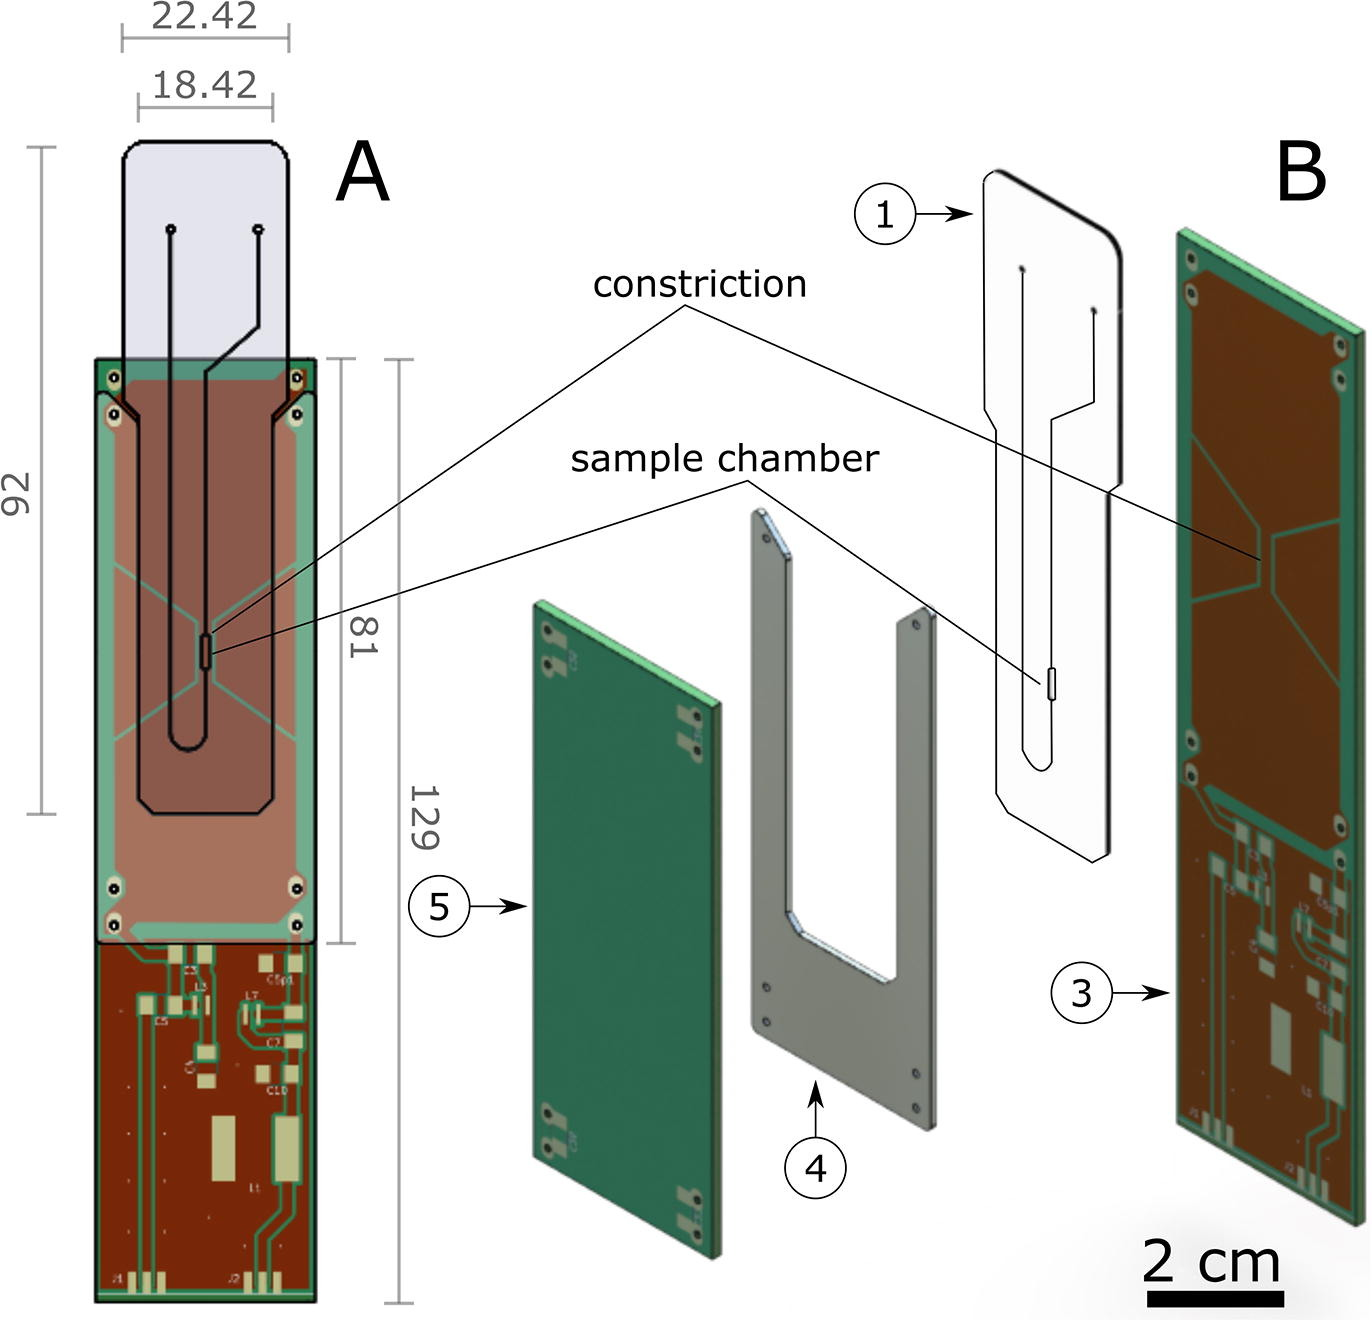
\includegraphics[width=\columnwidth]{Manvendra-Probe.jpg}
  \end{center}
  \caption{Drawings of the detector assembly and the microfluidic device (1). A: front view (dimensions in mm); B:
  exploded view. Spacer (4) ensures the alignment of the sample chamber with the constrictions on the PCB planes. In A,
  PCB plane 5 is hidden to show the orientation of 1 with respect to PCB plane 3. Thickness of each of the PCB planes
  is 1.52 mm and the copper layers on the PCBs is 35 $\mu~\text{m}$. Both the microfluidic device and the spacer are made from
  PMMA and have thickness of 0.9 mm and 1 mm respectively. Figure reproduced from\citep{RN164}}
  \label{fig:MVProbe}
\end{figure}
The main advantage of using this probe is the compatibility of the device with customisable chips allowing
a broad range of applications and enabling the marrying of practical NMR and some microfluidic capabilities which
few others allow\citep{RN165,RN166,RN167}. The limit of detection LOD for the TLP used is
1.4 nmol $\text{s}^{1/2}$ which comparitavely lower than detectors of a similar size and more similar to the LOD of
commercial cryo-probes mentioned previously. Where the probe is exceptional in terms of micro-detector is
the cLOD. Demonstrated in \fig{fig:cLOD}.
\begin{figure}
  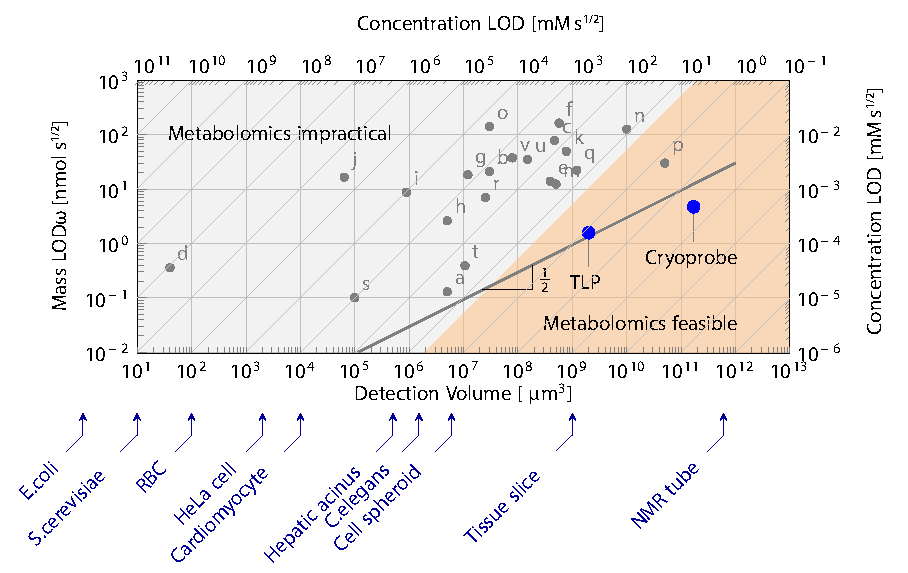
\includegraphics[width=\columnwidth]{sensitivity-ov.pdf}
  \caption{Plot comparing the limits of detection of previously design micro-NMR detectors. Letters
  a-t correspond to different authors as cited by Badilita \textit{et al.}\citep{Badilita:2011td} Letters u\citep{Meier:2014ds}
  and t\citep{RN165} represent more recent work. The probe used here is labelled at TLP and a comercial cyroprobe is shown for reference.}
  \label{fig:cLOD}
\end{figure}

For this work, the goal is not only to combine NMR detection and microfluidics, clearly that has been done before. However,
it is the combination of these two in a way that does not comprimise in either. That, in an NMR sense, means nLODs
comparible to macroprobes as well as sub 0.01 ppm line widths for true spectral resoltuion. This is displayed in
\fig{fig:cLOD}, the area shaded orange that we define as the 'metabolomics feasible' range is a maximum 5 mM $\sqrt{\text{s}}$
ensuring species present at 0.1 mM can be detected within less than 20 mins to a sufficient resolution. The TLP has a cLOD of
~ 1 mM $\sqrt{\text{s}}$ and can detect species at 0.02 mM in that time frame Whilst this is suitable for some metabolomic information to be
gained, however, the subtle changes in molecules present at less than 0.02 mM still evades us in the given time frame. Efforts towards
lowering the nLOD and cLOD are described in \ref{Parahydrogen}

%% !TEX root = ./Thesis.tex

\chapter{Microfluidc Droplet NMR}\label{Chapter:Droplets}

This chapter is an extended version of Hale. W, Rossetto. G, Greenhalgh. R, Finch. G and Utz. M, High-resolution
nuclear magnetic resonance spectroscopy in microfluidic droplets, \textit{Lab Chip}, 2018, \textbf{18}, 3018-3024 \citep{Hale:2018fv}

\section{Abstract}

In this chapter, a system that enables high-resolution NMR spectroscopy of microfluidic droplet
emulsions is discussed. Acquiring NMR spectra of emulsions is complicated by the magnetic
susceptibility mismatch between the phases and the chip material. In order to overcome these challenges a
2-part solution is needed. Firstly, air-filled structures are incorporated into the microfluidic chip design in order
to match the poly(methyl methacrylate) (PMMA) with the continuous phase (cyclohexane) susceptibility. Secondly, a $\ce{Eu^{3+}}$
complex is doped into the dispersed phase (water) in order to match the susceptibility of
the phases. High resolution spectra with linewidths of 3 Hz were obtained in the ideal case.
However, a serial dilution experiment that was used to obtain spectra of glucose droplets showed
the highly sensitive dependence of linewidth on Eu concentration.

\section{Introduction}

Droplet microfluidics is the field of microfluidic research that separates samples into discret droplets by dispersing one
immiscible fluid (dispersed fluid) in another (continuous fluid). In this way, samples can be manipulated freely in the lab-on-a-chip (LoC) system,
and problems due to viscous dispersion and cross-contamination
are avoided. In doing so, microdroplets of tuneable size and volume,
typically femto- to nanolitres, are produced at rate reported to be up to 44 kHz \citep{RN115}. Thorsen et al \citep{RN104}
reported one of the first droplet microfluidic devices. In the letter, they show how one can use microfluidic channels to
generate mono-disperse microemulsions by shearing water into a perpendicular flow of oil. By varying the ratio of the pressures
driving the flow of each fluid they produce droplets that range in diameter from 10 $\mu\text{m}$ to 60 $\mu\text{m}$.

Droplets have since emerged as a versatile tool finding wide ranging applications in areas
such as microcapsule synthesis \citep{RN105}, crystal growth \citep{RN106}, chemical reactions
\citep{RN114}, cell/organism encapsulation \citep{RN107,RN108, RN113}, PCR \citep{RN109,
RN110}, and Protein studies \citep{RN111, RN112}. These applications are diverse owing to many
advantages that microfluidic droplets possess: limited cross contamination; high production
rates; large surface area to volume ratio; small reagent volumes; and independent control of
each droplet \citep{RN102}.

Droplet generation can, broadly speaking, be divided into two categories. These are active
and passive generation methods. Active methods are defined as applying additional force to
the device to create droplets such as electric \citep{RN116}, magnetic \citep{RN117} or
centrifugal \citep{RN11} or by modifying intrinsic forces by tuning fluid
velocity \citep{RN58}. Passive methods rely on the inherent instability of the liquid-liquid
interface when mixing two immiscible fluid in order to generate droplets \citep{RN120, RN121,
RN122}. Zhu and Wang \citep{RN123} have published an in-depth review of the various methods of
droplet generation as well as the equations that govern them.

Here, active droplet generation is used in the form of fluid velocity variation. Two
syringe pumps were employed that allowed separate manipulation of flow rates of the dispersed
and continuous fluid. The dispersed and continuous phase are co-flowed to the the droplet
generation point. By using this method, one can control the production rate and size of the
droplets. Droplets of size ~100 $\mu\text{m}$ in diameter and a rate suitable enough to fill
the sample chamber. If the flow is too fast the droplets have a very low residence time and
there is never enough build up to perform an experiment. If, however, the flow is too slow
the droplets that are formed are too big and inconsistent for any kind of reliable
experimentation.

As discuss in chapter 2, nuclear magnetic resonance (NMR) as a spectroscopic technique has two chief advantages. It is
non-invasive and non-destructive which makes it ideally placed to study living systems without
destroying them. Indeed, NMR and magnetic resonance imaging (MRI) are both methods actively
employed in metabolomics \citep{RN124}, drug discovery \citep{RN125} and cancer
imaging \citep{RN126}. The nature of NMR means that one can glean quantitative, system
level information in one experiment without the need for chemical tags. In a microfluidic
context, where fluorescence \citep{horrocks2015fast, schlimpert2016fluorescence}, or
mass spec \citep{redman2016characterization,choi2016digital}, are often the methods of choice
for spectroscopy NMR can be used in parallel to these and contribute to a better understanding of the system.

In this work, the possibility to obtain high-resolution NMR spectra from
small volumes of droplet emulsions on a chip is explored.
Integration of high-resolution NMR spectroscopy with microfluidic systems is
challenging for a number of reasons.
On the one hand, small sample volumes place stringent demands on detector
sensitivity \citep{Badilita:2011td,Zalesskiy:2014hi}
This has recently been addressed with the design of
highly efficient planar NMR microcoils \citep{Spengler:2016km} and
transmission line resonators \citep{Finch:2016gv}
Another challenge is the preservation of high spectral
resolution, which depends on a highly homogeneous magnetic field
over the sample volume. Differences in magnetic susceptibility
between the materials used for the microfluidic chip
and the sample fluid, as well as the materials and geometry
of the probe assembly, lead to a demagnetising field
that varies continously over the sample volume. Typical diamagnetic
volume susceptibilties range from about
$-11$~ppm to about $-5$~ppm (in SI units); \citep{Kuchel:2003ip,Durrant:2003kv}
differences of the order of several ppm are therefore commonplace.
Unmanaged, they lead to
broadening of NMR spectral lines over a ppm or more, which
corresponds to a severe loss of resolution in $\ce{^1H}$ liquid
state NMR.

Managing susceptibility differences for an emulsion of droplets on a
microfluidic chip adds additional complexity, since three different materials
are now involved: the chip, the continuous phase, and the droplet phase,
all with different susceptibilities.
This can be mitigated in a two-step approach,
which is based on the observation that most organic solvents in use
as continuous phases for droplet microfluidics are less diamagnetic than
water.
First, the susceptibility difference between the chip and the continuous phase
are compensated by shimming structures that are added to the
chip design. Then, the susceptibility of the aqueous droplet phase is matched
to that of the continuous phase by adding a paramagnetic solute.

\subsection{Susceptibility}

Magnetic susceptibility, $\chi_V$, is a measure of how much a material will become magnetized in an
applied magnetic field, broadly, this allows a classification of most materials as para- ($\chi$>0)
or dia- ($\chi$<0) magnetic. Materials used in this work are listed in Table \ref{tab:suscept}.

The magnetization of the material is given by the equation $\mathbf{M} = \chi_V \mathbf{H}$
where $\mathbf{M}$ is the magnetisation of the material and $\mathbf{H}$ is the magnetic field. In
\citep{RN118}, a derivation of how the susceptibility can affect the magnetic field around a sample
and influence its spectra is given.

In the absence of currents Ampere’s law requires that $\nabla \times \mathbf{H} = 0$. The magnetic field $\mathbf{H}$
can then be expressed by a scalar magnetic potential $U$ as:
\begin{equation}
\mathbf{H} = -\nabla U
\end{equation}

To describe an object being inserted into a magnetic field we split the potentials as $U = U_{0}  + U_{d}$, where $U_{0} = H_{0}z$ represents the original homogeneous field, and
$\mathbf{H}_d = - \nabla U_{d}$ is the field generated by the magnetic dipoles induced in the inserted object (sometimes referred to as demagnetising field). The magnetic field $H_{0}$, which we assume to be along the z-axis, arises from the superconducting coil

 The macroscopic magnetic induction $\mathbf{B}$ is given by:
\begin{equation}
  \mathbf{B} = \mu_{0}(\mathbf{H}+\mathbf{M})
\end{equation}

where $\mu_{0} = 4\pi\times10^{7}~\text{VsAm}^{-1}$ denotes vacuum permeability. With Gauss' law $\nabla \cdot \mathbf{B} = 0$ this becomes:

\begin{align}\label{eqn1}
  \mathbf{B} =& \mu_0(-\nabla(U_0 + U_d) + \mathbf{M})\\
  \nabla\cdot\mathbf{B} =& \mu_0(-\nabla^{2}(U_0 + U_d) + \nabla\cdot\mathbf{M})
  \nabla^{2}U_{d} = \nabla \cdot \mathbf{M}
\end{align}

We assume that the object consists of a number of spatial domains characterised by a
locally constant magnetic susceptibility $\chi_{k}$. The magnetisation therefore, is a piecewise
constant,
\begin{equation}
  \mathbf{M}_{k} = \chi_{k}H_{0}\mathbf{e}_{z}
\end{equation}

the $\nambla\cdot\mathbf{M}$ term from Eqn. \ref{eqn1} vanishes everywhere except at domain boundaries. The magnetic
field satisfies the boundary conditions\citep{Jackson:2007uq}

\begin{equation} \label{eqn2}
  (\mathbf{H}_{d2} - \mathbf{H}_{d1}) \times \breve{\mathbf{n}} = 0,
\end{equation}
\begin{equation} \label{eqn3}
    (\mathbf{H}_{d2} - \mathbf{H}_{d1}) \cdot \breve{\mathbf{n}} = H_{0}(\chi_{2} -
    \chi_{1})\mathbf{e}_{z}\cdot\breve{\mathbf{n}},
\end{equation}

where $\breve{\mathbf{n}}$ denotes the surface norml from material 1 to material 2. Equations \ref{eqn1}, \ref{eqn2}
and \ref{eqn3} are formally solved by:

\begin{equation}\label{eqn:Magnetostatic}
  U_{d}(\mathbf{r}) = \frac{H_{0}}{4\pi}\int_{\delta_{12}}\frac{\breve{\mathbf{n}}\cdot\mathbf{e}_{z}(\chi_{2}-\chi_{1})}{\sqrt{(\mathbf{r}-\mathbf{r'})^{2}}}dS,
\end{equation}

where $dS$ is an infinitesimal surface element, and $\mathbf{r'}$ is the integration variable. If there are more than two materials involved, as there are in droplets where
there are three: the continuous phase; the water phase; and the PMMA, each boundary gives an additive contribution of the same form.

The resonance frequncy observed is proportional to the magnetic induction $\mathbf{B}_{ext}$
experienced by chemically equivalent nuclei within each domain. This induction is determined
by the outside field $H_{0}$ plus the induced magnetic dipoles of all molecules in the same domain except the molecule carrying
the observed spin.\citep{Levitt:1996tg} In liquids and isotropic solids, the external magnetic induction differs from the macroscopic $\mathbf{B}$ as:

\begin{equation}
  \mathbf{B}_{ext}-\mathbf{B} = \frac{2\mu_{0}\chi_{s}}{3}\mathbf{H}_{0}
\end{equation}

The magnetic induction relvant for the Larmor precession of nuclear spins in the sample is therefore

\begin{equation}\label{eqn:LarmorSpins}
  \mathbf{B}_{ext} = \mu_{0}H_{0}(1 + \frac{\chi_{s}}{3})\mathbf{e}_{z} - \mu_{0} \nabla U_{d}
\end{equation}
Since $\chi$ is a piecewise constant, the $\mu_{0} \nabla U_{d}$ term contributes to continuously varying fields
and therefore any line broadening seen in the spectrum, whereas the $\mu_{0}H_{0}(1 + \frac{\chi_{s}}{3})\mathbf{e}_{z}$
produces a bulk magnetic susceptibility shift (BMS) of the resonance line.


\subsection{Matching susceptibilities in emulsions}


Matching susceptibilties of materials is a problem in microfluidic NMR. Fortunatey, the susceptibilities
of the materials used are typically similar as
in most of our experiments, the solvent is water and the chip material is PMMA.

When the susceptibilities are mismatched, as they are in droplets, this can cause inhomogeneities in
the magnetic field, this shifts the resonances and broadens the lines in the spectra rendering them
useless. For any kind of useful NMR, the magnetic field needs to be very homogeneous with most commercial
superconducting magnets achieving homogeneities of a few parts per billion. In microfludic devices,
air-filled shim structures have been utilised to match suceptibilities between chip construction material
and fluid. Utz and co workers \citep{RN118}
have shown that susceptibility mismatches can be
compensated for by installing such shim structures around the NMR sensitive region, to produce an
equal and opposite demagnetising field to the one caused by the solution, well
resolved spectra can be taken of glucose dissolved in the mismatched liquid.
\begin{figure}
  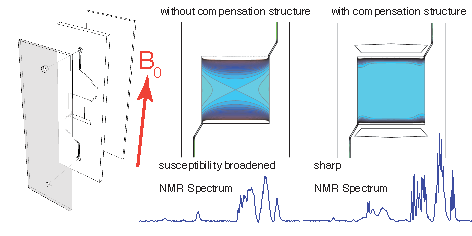
\includegraphics{struct-shim-toc-sm.pdf}
  \caption{Summary graphic of the work in \citep{RN118}. This shows how the NMR spectrum of glucose
  changes in a suscpetibility mismatched chip but by cuting shimstructures around the sample chamber high resolution
  NMR is still possible despite the mismatches.}
  \label{ShimStructUtz}
\end{figure}

This work, combines both structural shimming and chelated lanthanide doping, to glean high resolution NMR spectroscopy
from a microfluidic droplet emulsion. The system is comprised a PMMA chip, an aqueous dispersed phase, and a cyclohexane
continuous phase. As mentioned the PMMA and water are susceptibility are quite similar. The cyclohexane, however, is matched to
neither. Hence,  for all materials and solvents to be matched, structural shimming is employed to match the PMMA
to the cyclohexane and a chelated lanthanide $\ce{[Eu(DTPA)]}^{2-}$  will be used to match the water susceptibility.

In emulsions, susceptibility differences between the oil and aqueous phases
lead to similar line broadening \citep{Kuchel:2003ip} NMR spectroscopy is extensively
used to characterise emulsion droplet size distributions using pulsed
field gradient methods \citep{VANDENENDEN:1990ck,FOUREL:1994jv,
Hollingsworth:2004iy,Hindmarsh:2005en,Johns:2009ib,Bernewitz:2011km,Lingwood:2012je}.
These methods do not require spectral resolution of individual
compounds other than the two solvents, and are therefore
unaffected by the susceptibility broadening. By contrast, high-resolution
NMR spectroscopy, with sufficient resolution to distinghuish multiple
compounds present in either of the two phases,
requires careful mitigation of the susceptibility differences. It has also been shown that susceptibility differences can
be compensated for in a liquid sample by doping of a chelated lathanide \citep{fabry1983effect}.
For example, Lennon \emph{et al.} demonstrated that the susceptibility mismatch between the inside and outside of deoxygenated red blood cells could be
compensated for by doping 3mM of dysprosium tripolyphosphate $\ce[{Dy(PPP)_2}]^{7-}$ into the extracellular fluid \citep{lennon1994hemoglobin}

\begin{figure}
  \begin{center}
    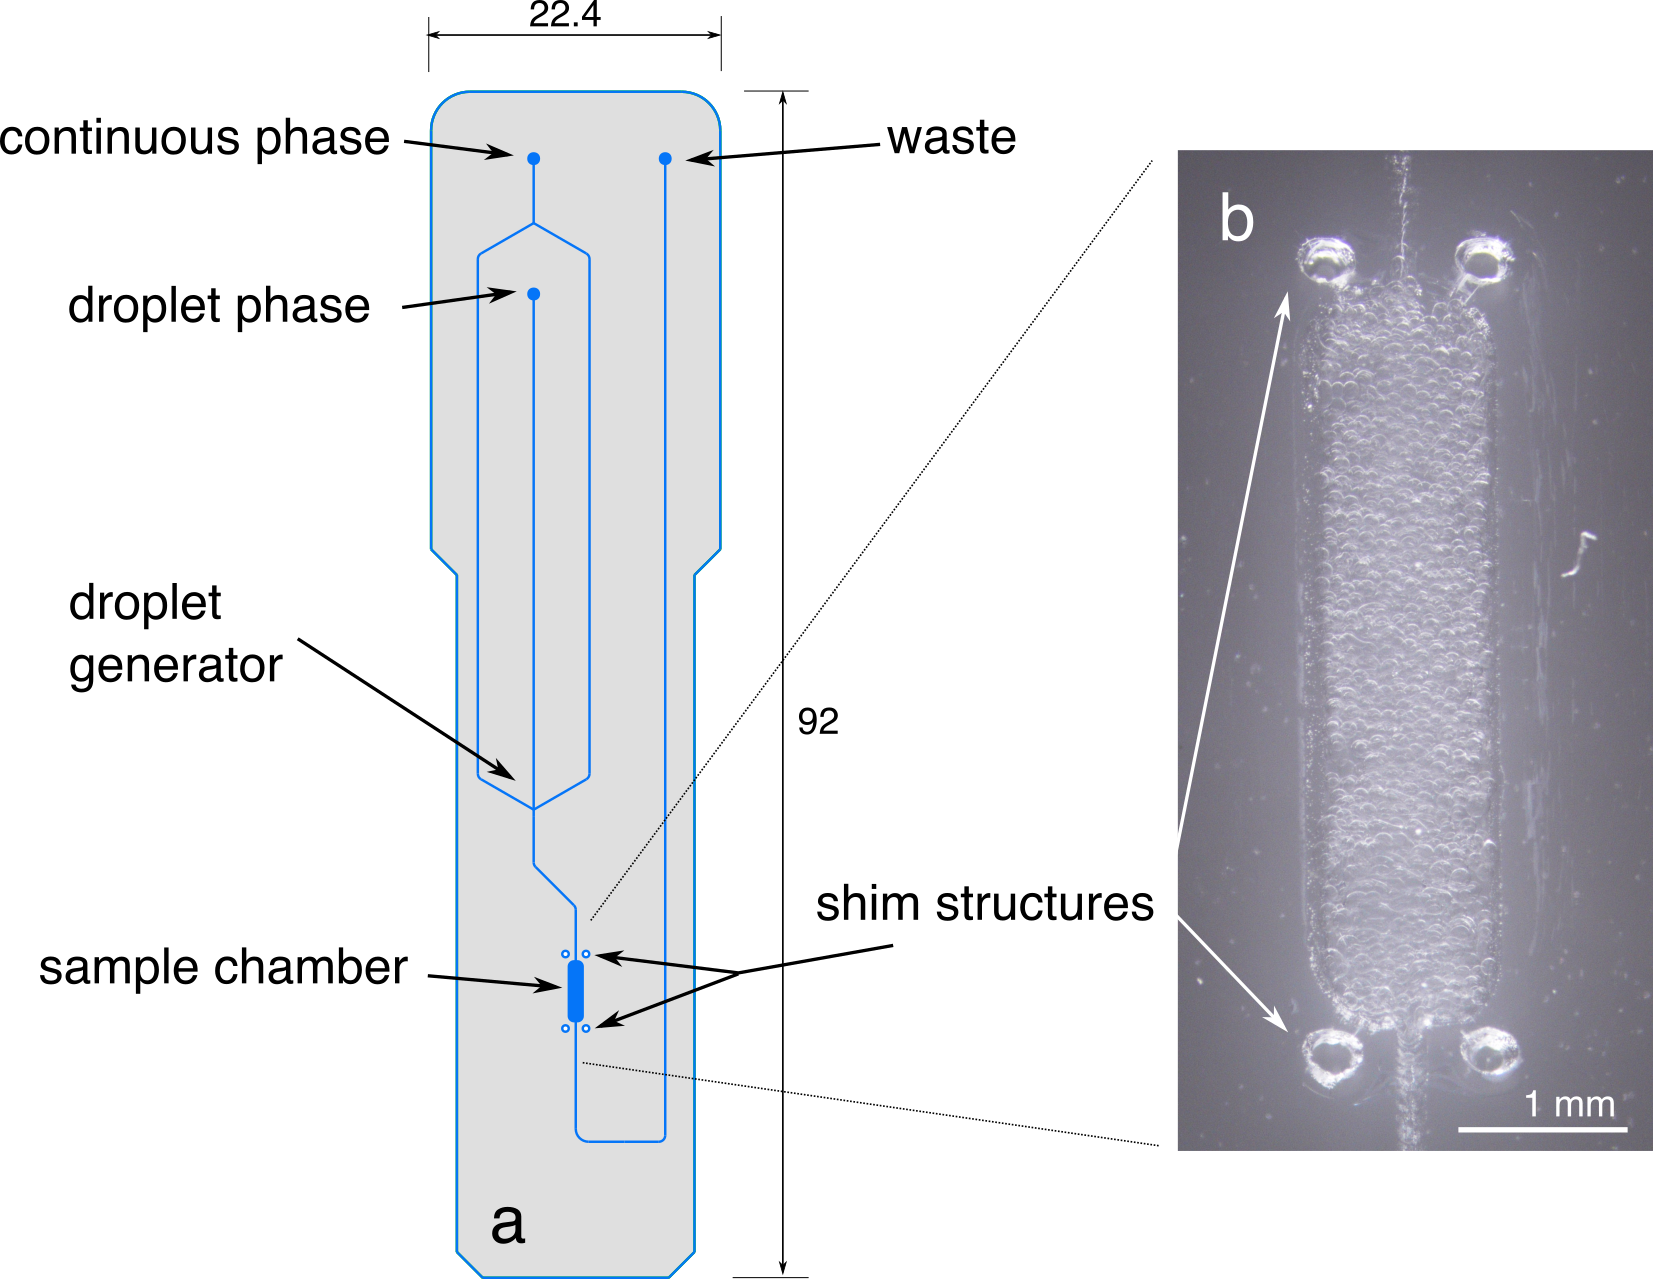
\includegraphics[width=0.8\columnwidth]{mu1y11-dnmr-fi-180421-chip-schematic}
  \end{center}
  \caption{Droplet chip design (left) and detail micrograph of the sample chamber
  area filled with droplets (right). Some droplets are also visible in the
  entrance and exit channels.}
  \label{fig:chip-design}
\end{figure}

It should be noted that in principle, the same effect could be achieved if
a diamagnetic dopant could be added to the continuous phase. However, while paramagnetic
dopants are easily available in the form of transition metal ions, no
effective diamagnetic dopants exist in the literature.

$\ce{Eu^{3+}}$ complexes are paramagnetic, and are frequently used as
shift agents in NMR spectroscopy. Unlike other lanthanide ions such
as $\ce{Gd^{3+}}$ or $\ce{Ho^{3+}}$, which are powerful nuclear relaxation
agents, $\ce{Eu^{3+}}$ has only a minimal
effect on nuclear magnetic relaxation due to its extremely
short electron spin-lattice relaxation time \citep{Peters:1996bj} Addition of
millimolar quantities of $\ce{Eu^{3+}}$ to aqueous solutions
therefore does not cause significant relaxation line broadening, but changes
the bulk magnetic susceptibility of the solution proportionally
to the $\ce{Eu^{3+}}$ concentration. It is therefore possible
to adjust the susceptibility difference in a droplet emulsion
by adding a $\ce{Eu^{3+}}$ complex that selectively dissolves in (or at least
strongly partitions to) the aqueous phase.


\begin{table}
\begin{center}
    \caption{Bulk magnetic susceptibilities}
    \label{tab:suscept}
    \begin{tabular}{lcc}\hline\hline
      \emph{Compound} & $\chi_V/10^{-6}$ (SI) & Ref \\ \hline
      water           & $-9.05$               &    \citep{Rumble:2017tp}  \\
      cyclohexane     & $-7.640$              &    \citep{Rumble:2017tp} \\
      PMMA            & $-9.01$               &    \citep{Wapler:2014es}\\
      Air             & $+0.36$               &    \citep{Bakker:2006eea} \\ \hline\hline
    \end{tabular}
\end{center}
\end{table}



\begin{figure}
  \begin{center}
    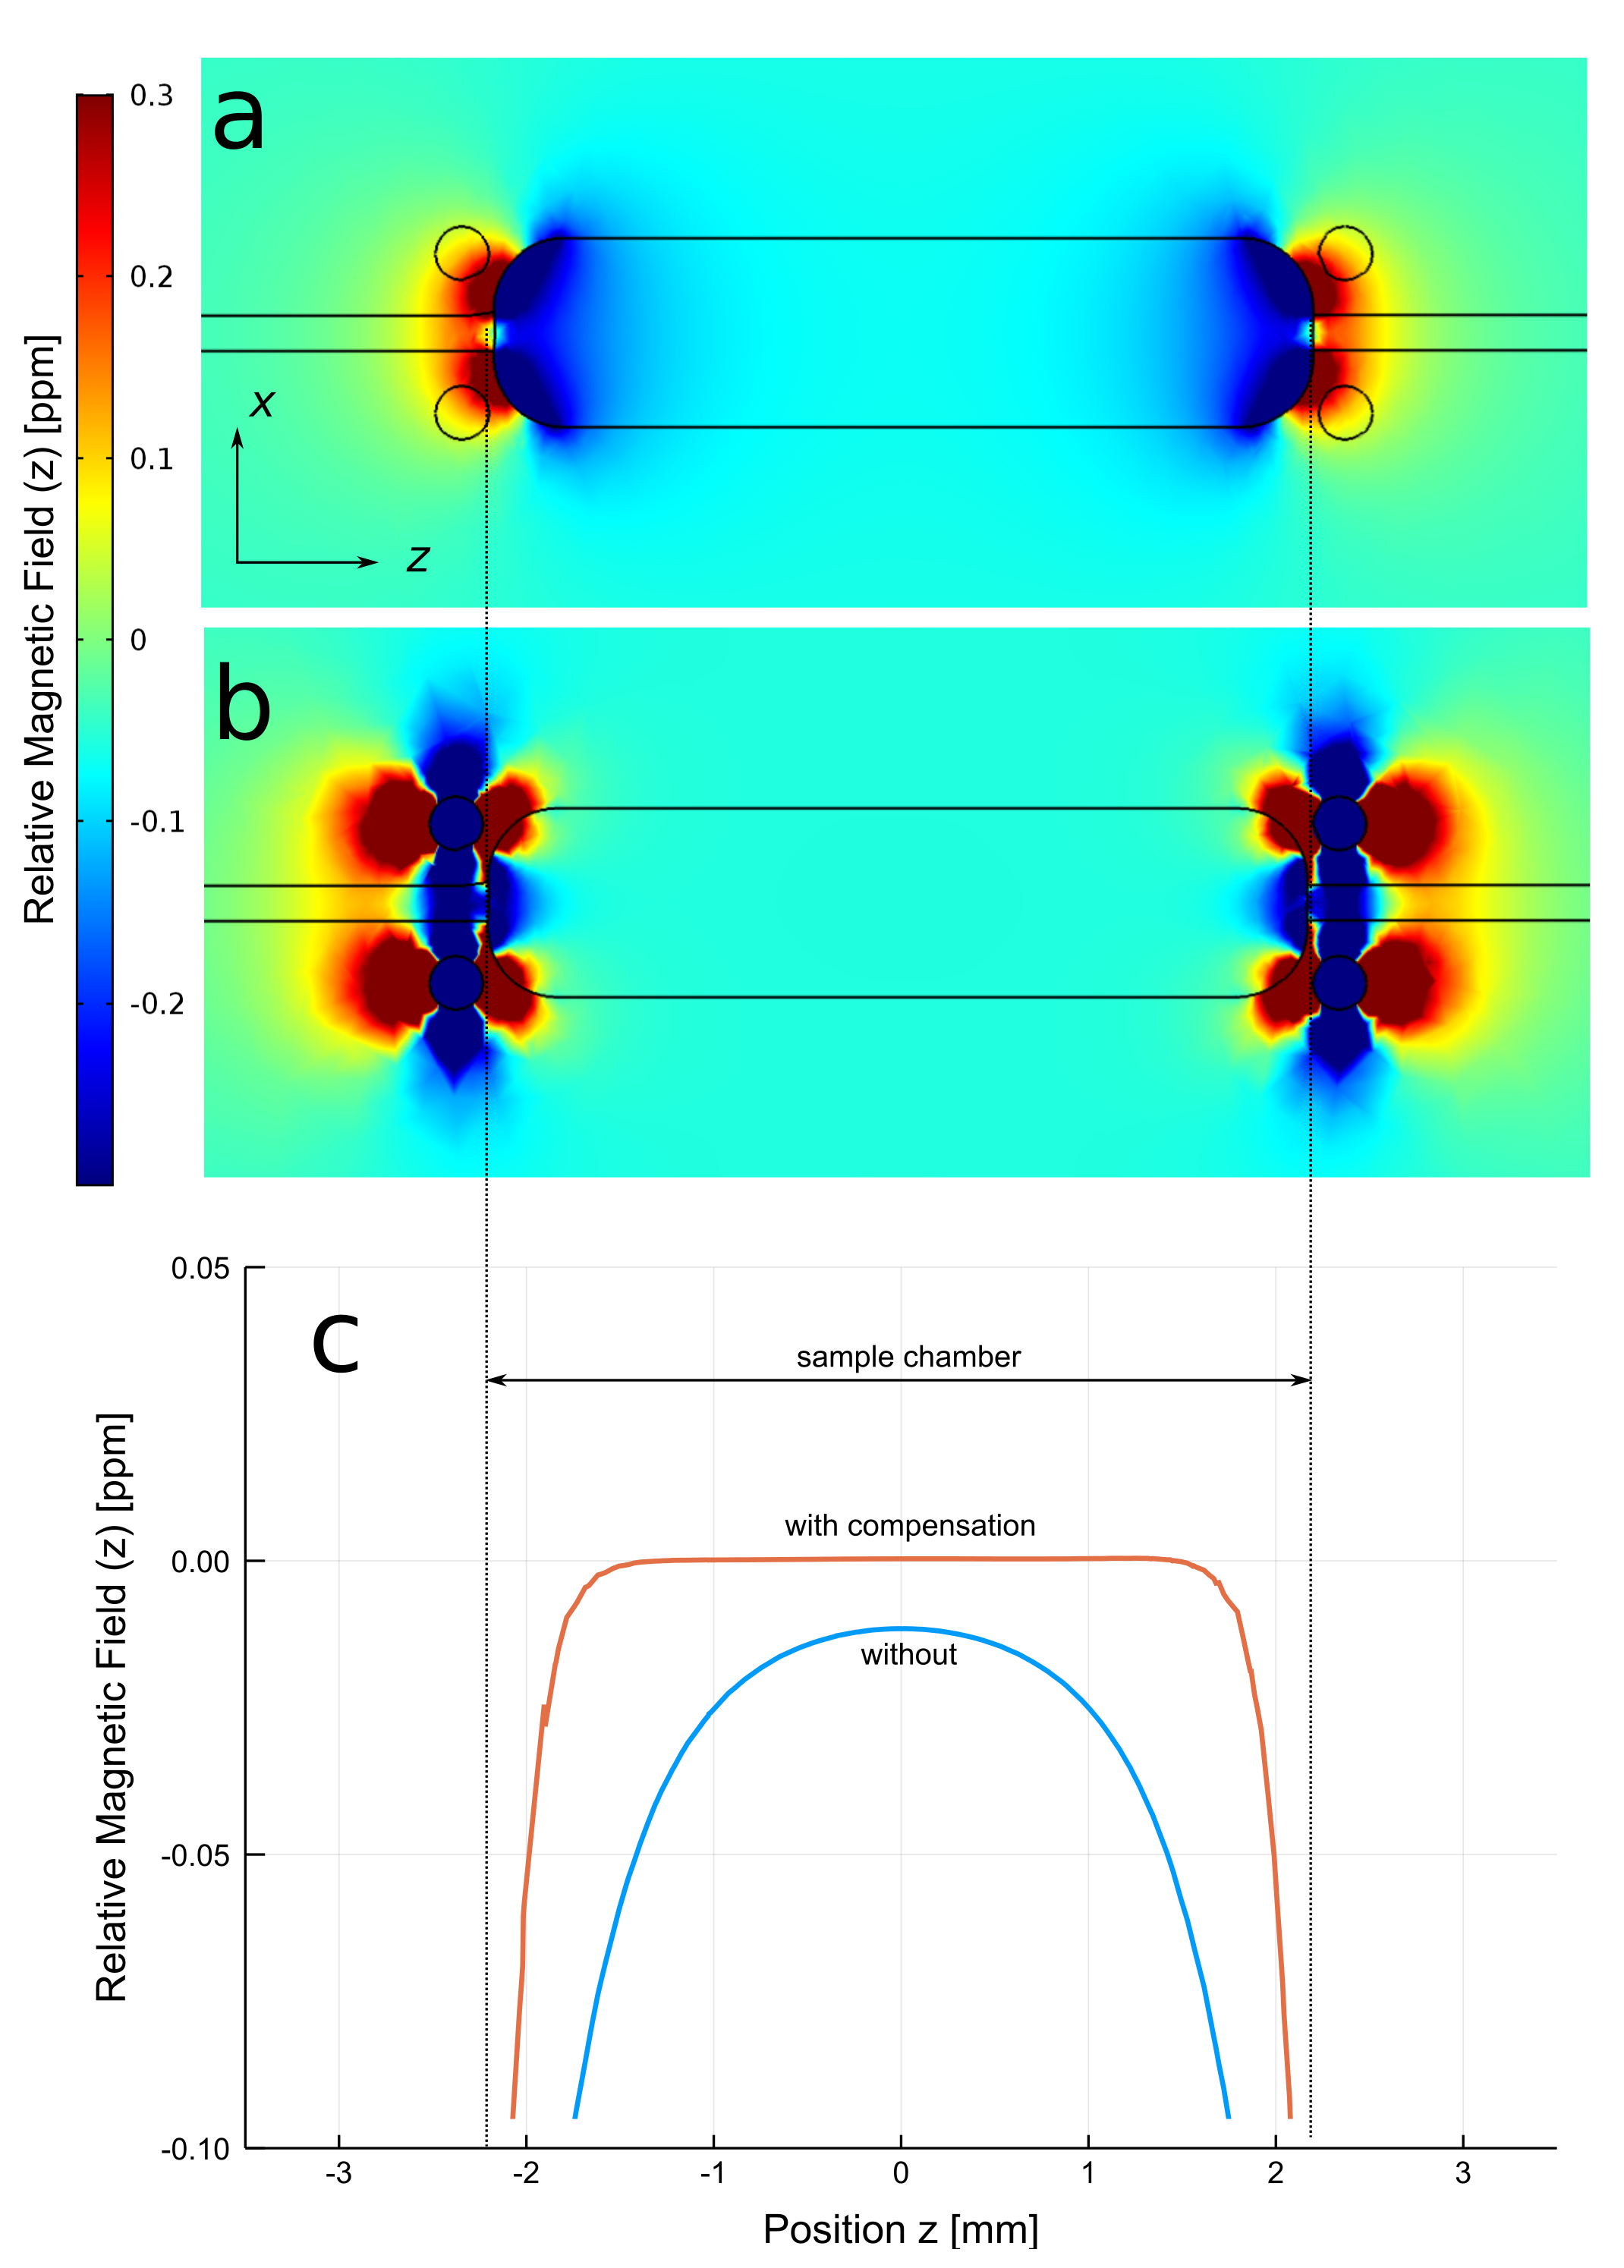
\includegraphics[width=0.8\columnwidth]{mu1y11-dnmr-fi-180421-chip-FEM.png}
  \end{center}
  \caption{A: Finite element simulation of relative magnetic field distribution in an uncompensated chip (circular structures filled with PMMA) filled with cyclohexane
      and B: a compensated chip filled with cyclohexane; C: a linear plot of relative magnetic field along the z-axis through the middle of the sample chamber.
    }
  \label{fig:FEM-chip}
\end{figure}


\begin{figure}
  \begin{center}
    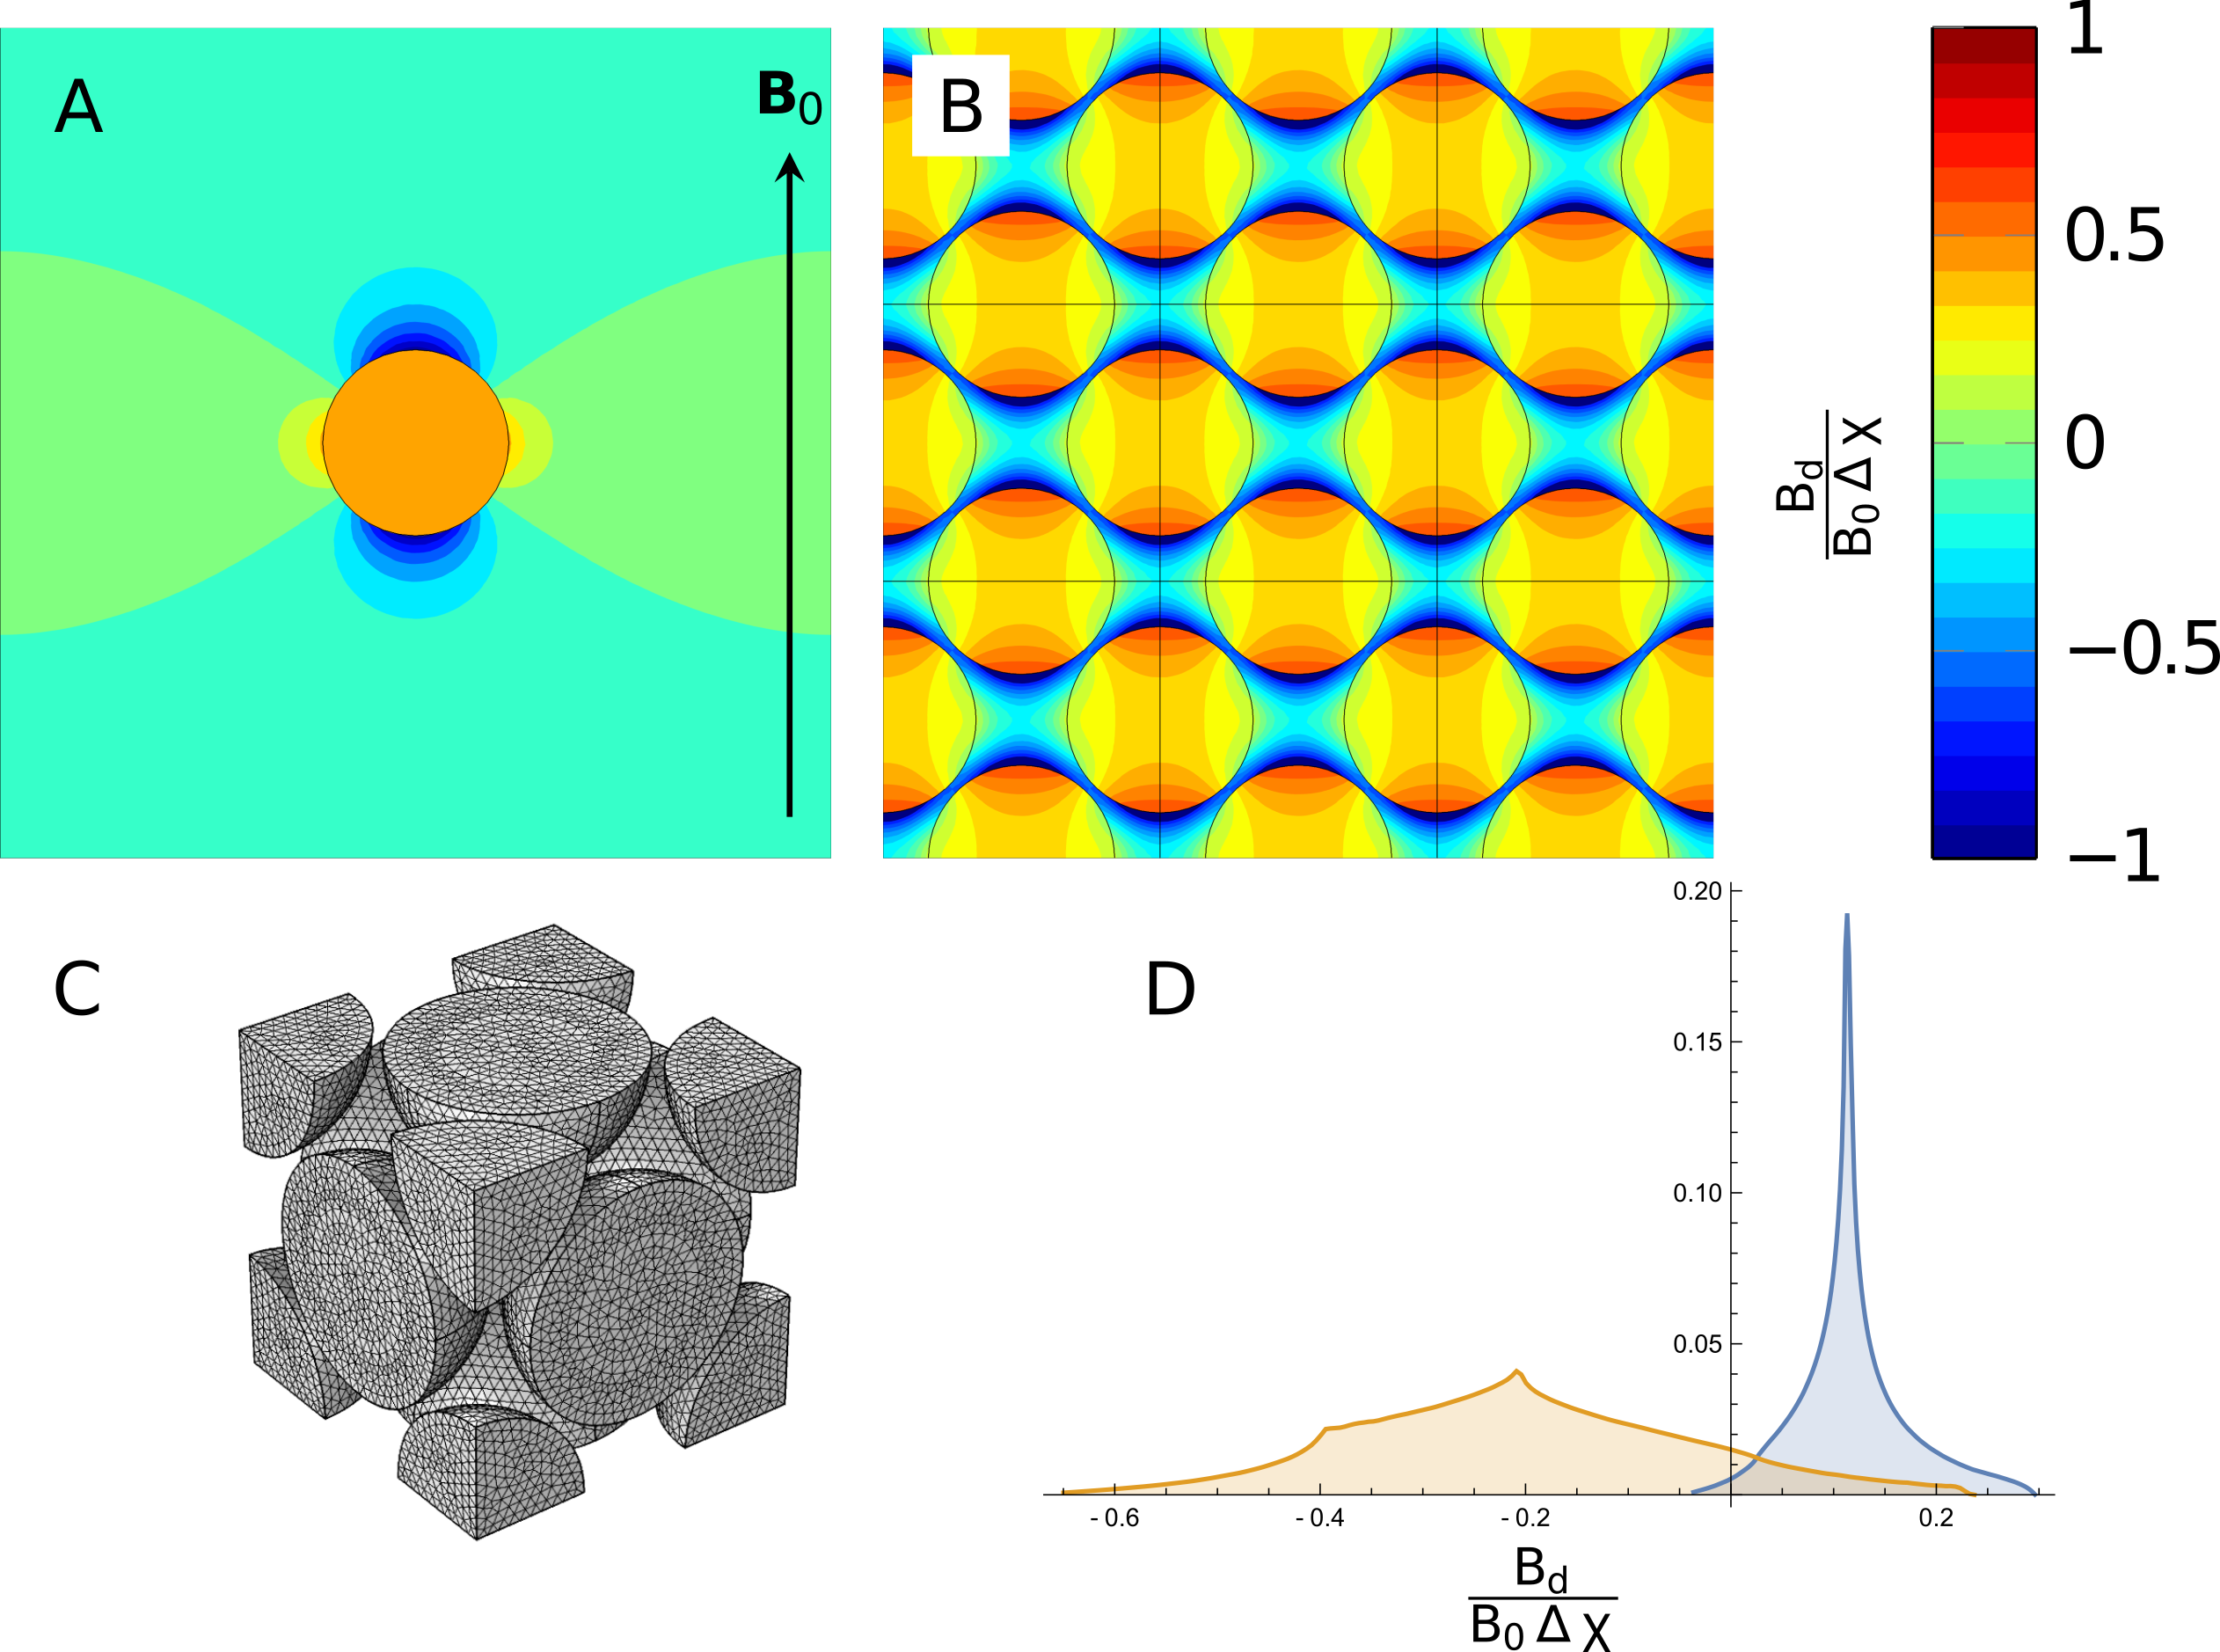
\includegraphics[width=\columnwidth]{mu1y11-dnmr-fi-180629-fcc-simulated}
  \end{center}
  \caption{A: Finite element simulation of magnetic field distribution in droplets.
      $z$-component of the reduced magnetic field $H_\text{red}$ in an isolated spherical droplet
      and B: in a face-centred cubic arrangment of droplets; C: FEM mesh used
      to calculate the result shown in B; D: histograms of the $z$-component
      of the reduced magnetic field in the continuous (orange) and in the droplet (blue) phase
      in the FCC arrangement.
    }
  \label{fig:FEM-fcc}
\end{figure}


In the present work, the diethyl-triamine pentaacetate (DTPA) complex
of $\ce{Eu^{3+}}$, $\ce{Eu[DTPA]^{2-}}$ is used. As an ion species, it is readily soluble
in aqueous media, while exhibiting only negilgible solubility in apolar organic
solvents. Microfluidic chips are fabricated from poly methyl methacrylate (PMMA).
By a fortunate coincidence, the suceptibilities of PMMA and
water are very close to
each other (Table \ref{tab:suscept}).  NMR lines
in microfluidic devices made from PMMA are therefore narrow
if  aqueous samples are used, provided that the boundaries of the chip and the environment
are either aligned with the external magnetic field, or are kept sufficiently
remote from the detection area. By contrast, most organic solvents are
considerably less diamagnetic than water, as exemplified by the
case of cyclohexane, which has been used in the present study.

In the remainder of this chapter,
finite element calculations are used to estimate
the NMR line widths expected in a droplet emulsion
depending on the susceptibility mismatch.
The results are then compared to experimental
line widths obtained with varying concentrations
of $\ce{Eu[DTPA]^{2-}}$ in the aqueous phase. Finally,
narrow NMR lines are obtained by
combining structural shimming \citep{Ryan:2014hl} with
susceptibility matching, and demonstrate that this
approach can be used to obtain a high resolution of glucose contained within the compensated droplets.
The chip used in this work is shown in \fig{fig:chip-design}. It consists of a sample
chamber in the centre of the chip, which is designed to line up with
the sensitive area of a transmission-line
micro-NMR detector \citep{Finch:2016gv}, and a convergent flow droplet
generator. The aqueous phase and the continuous
phase are fed into the two ports at the top. Droplets are
formed and transported downstream into the sample chamber.
 The chamber is surrounded by four shim structures, which are circular
 shaped cutouts filled with air. They have been designed to compensate
 for the difference in susceptibility between the chip material (PMMA)
 and the oil phase (cyclohexane) as shown in \fig{fig:FEM-chip}. The operation of the chip is shown
 on the right side of \fig{fig:chip-design}; droplets of about 100~$\mu$m diameter are formed and
 fill the sample chamber.



\begin{figure}
  \begin{center}
    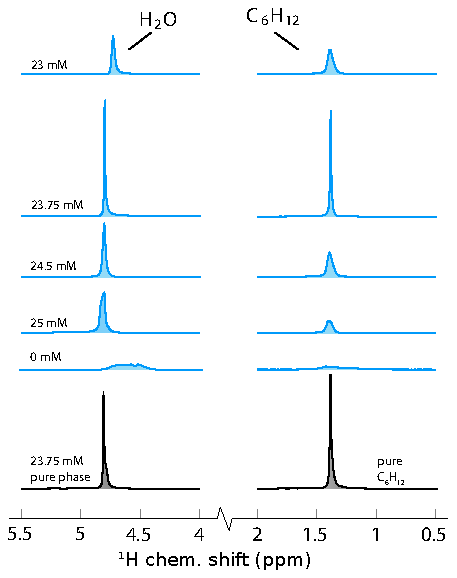
\includegraphics[width=0.7\columnwidth]{normalised-new-droplet-spectra}
  \end{center}
  \caption{$^1$H NMR line shapes of water (left) and cyclohexane (right) of a
  water in cyclohexane emulsion as a function of $\ce{Eu[DTPA]^{2-}}$ concentration
  in the aqueous phase normalised to the sharpest peak. The spectra given in black are the pure phase spectra produced by the same chip.
  }
  \label{fig:droplet-spectra}
\end{figure}


\begin{figure}
  \begin{center}
    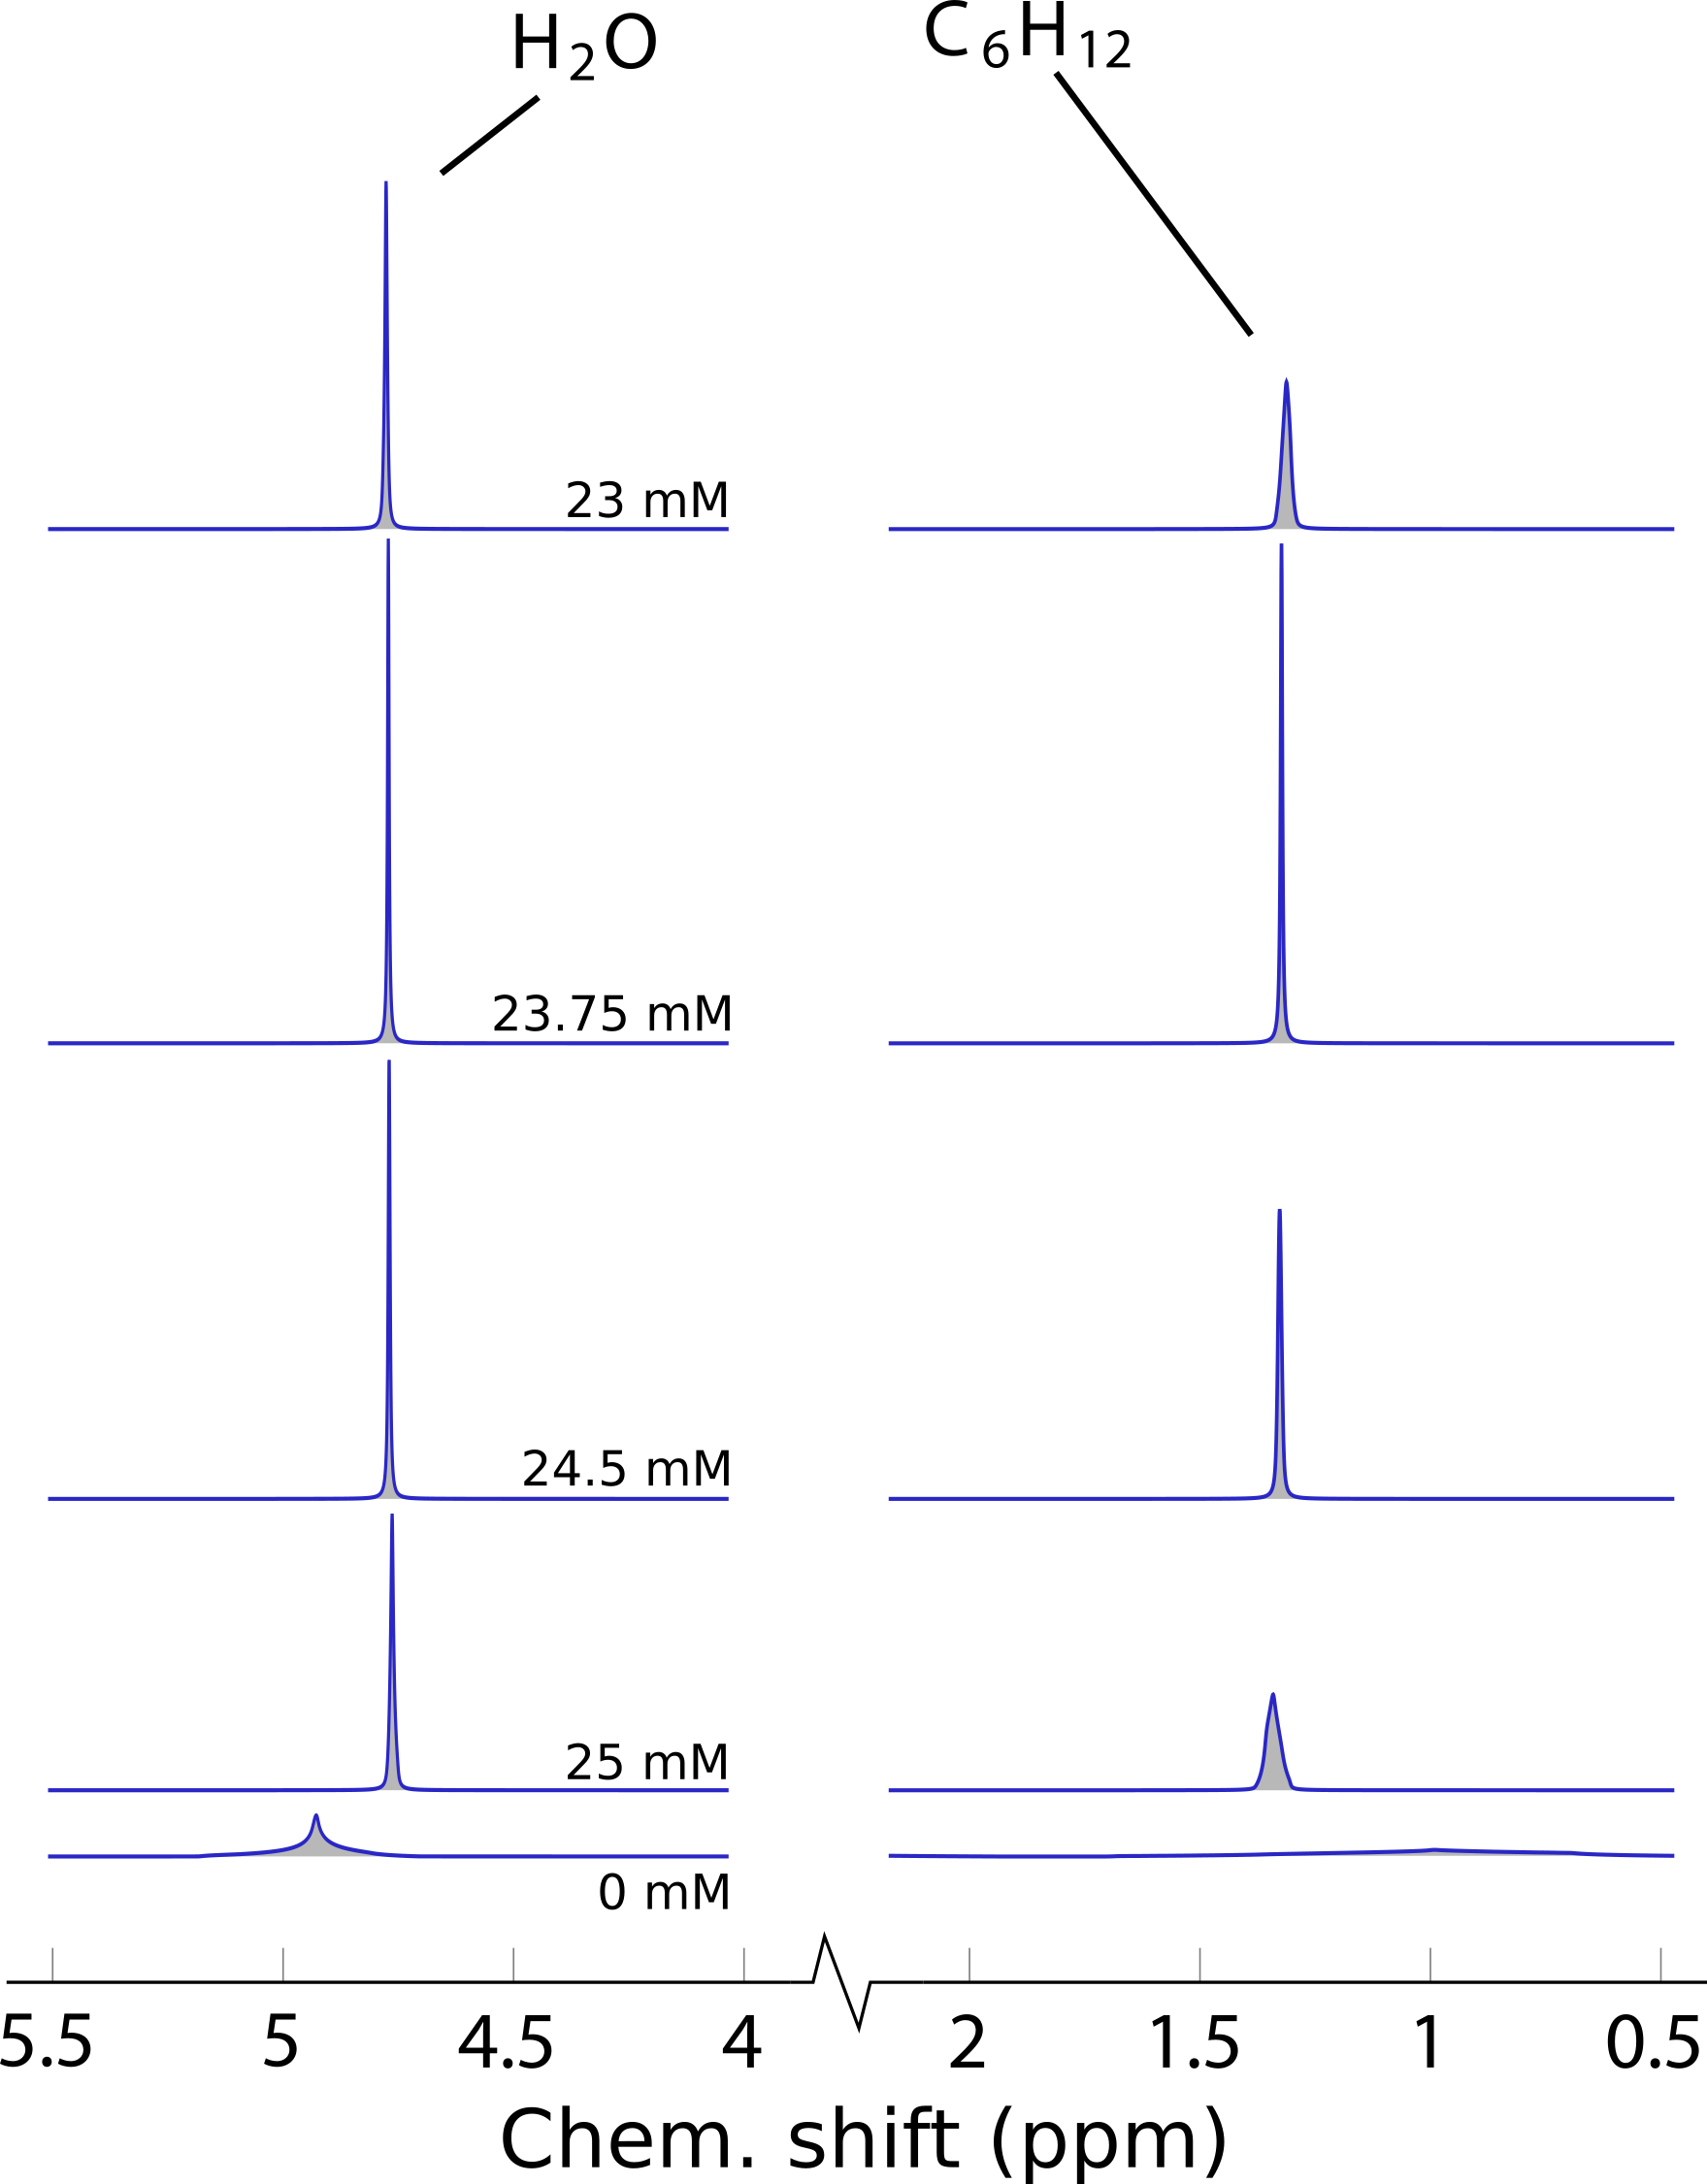
\includegraphics[width=0.7\columnwidth]{mu1y11-dnmr-fi-180622-simulated.png}
  \end{center}
  \caption{Predicted $^1$H NMR line shapes of water (left) and cyclohexane (right) of a
  water in cyclohexane emulsion as a function of $\ce{Eu[DTPA]^{2-}}$ concentration
  in the aqueous phase.
  }
  \label{fig:predicted-spectra}
\end{figure}




\section{Materials and Methods}

Microfluidic chips of the design shown in \fig{fig:chip-design}
were fabricated from PMMA sheet material by
laser cutting, and subsequent bonding of layers with a plasticiser
under heat and pressure \citep{Yilmaz:2016fx}. The chips consist of a
top and bottom layer of 200~$\mu$m thickness each, and a middle layer of
500~$\mu$m. Fluid channels upstream from the flow-focussing droplet
generator were scored into the middle layer at low laser power to a depth
of about 100~$\mu$m. Downstream from the droplet generator, the channels and
the sample chamber were cut through the 500 $\mu$m middle layer by increased
laser power, as were the shimming structures. The chips were connected to
a pair of Cole-Palmer 200-CE syringe pumps for droplet generation.
A flow rate of 20~$\mu$l/min was typically used for the continuous
phase and 4~$\mu$l/min for the aqueous droplet phase.
The continuous phase consisted of cyclohexane (Sigma-Aldrich)
with 0.5\% w/v of span-65 (sorbitan
tristearate, Sigma-Aldrich) as a surfactant to ensure droplet stability.
The cyclohexane/span solution was kept in a water bath at 30$^\circ$C
for at least 2h to ensure complete dissolution of the surfactant.
Prior to use, all solutions were left to equilibrate at a controlled room temperature
of 25$^\circ$C for at least 4h.
Steady state conditions were ensured by letting the droplet generation run until
the volume inside the chip had been exchanged at least five times. The
chip was then disconnected from the syringe pumps, and the connection
points sealed prior to insertion of the chip into the NMR probe.

NMR measurements were carried out on a Bruker AVANCE III
spectrometer equipped with an Oxford wide bore magnet operating at 7.05 Tesla,
corresponding to a $\ce{^1H}$ Larmor frequency of 300 MHz. A home-built NMR probe
based on a transmission-line detector was used \citep{Finch:2016gv}
It accommodates microfluidic chips of the shape shown in \fig{fig:chip-design}.
In the present work, the probe was doubly
tuned to allow irradiation both at 300 MHz for $\ce{^1H}$ and at 75 MHz for
$\ce{^{13}C}$. Details of the electronic and mechanical design of the
probe are given in Ref.~\citep{Finch:2017vb}.

NMR spectra were obtained at an RF nutation frequency of 66 kHz for
$\ce{^1H}$, corresponding to 90 degree pulse length of
3.8 $\mu$s. Shimming was first performed on a sample of pure cyclohexane
in an identical chip, these resulting values were used throughout all subsequent experiments with
minor adjustments being made to linear shims (X,Y,Z) before each experiment to minimise line width. NMR spectra were acquired using Bruker spectrometer software (TopSpin 2.0),
and were processed using home-built scripts written in \textit{Julia}. \citep{Bezanson:2017gd}
20~mM of 4,4-Dimethyl-4-silapentane-1-sulfonic acid (DSS, Sigma Aldrich) was added to the aqueous phase
as a chemical shift standard.

MRI gradient echo images of the sample chamber were obtained using ParaVision software and the fast low-angle shot (FLASH) pulse program. Flip angles of 30$^\circ$ were employed as well as a repetition time of 600 ms; 8 scans were averaged for each image. Two images were acquired for each field map at echo times of 6 and 10ms, respectively. The data was processed using home built software in \textit{Mathematica}.

$\ce{Eu[DTPA]^{2-}}$ solutions were prepared  from a $82.2\pm0.25$~mM
stock solution, which was prepared by adding 1 g of $\ce{EuCl_3}$
(Sigma Aldrich) to a 50 mL volumetric flask. Separately,
3.93 g of diethylenetriaminepentaacetic acid (DTPA, Sigma Aldrich)
and 1.99 g of NaOH (Fischer) were dissolved in 100 mL deionised (DI) water (Sigma Aldrich) .
An equimolar amount of the DTPA solution was added to the $\ce{EuCl_3}$ solution. The pH of this solution was then adjusted by addition of 2M NaOH solution dropwise until a neutral pH was attained.
This was then topped up to 50 mL using DI water.

Finite element calculations of field distributions in emulsions
 were carried out using COMSOL Multiphysics with the "magnetic fields, no currents" (mfnc) physics module.
Optimisation of the shim structures was done with COMSOL Multiphysics \citep{comsolmp} Starting from a SolidWorks model
of the chip design, which was also used as a basis for production of the devices using
a laser cutter, a finite element model was assembled and meshed. The shim structures consist
of four symmetrically arranged circular holes through the middle layer of the three-layered
devices. The positions and the diameters of these
holes were optimised using a Nelder-Mead simplex algorithm. At each iteration, the magnetic
field distribution inside the sample chamber was calculated using the mfnc physics module.
The square norm of the second derivative of the $z$-component of the magnetic field was integrated
over the volume of the sample chamber, and was used as optimisation target.

\begin{figure}
  \begin{center}
    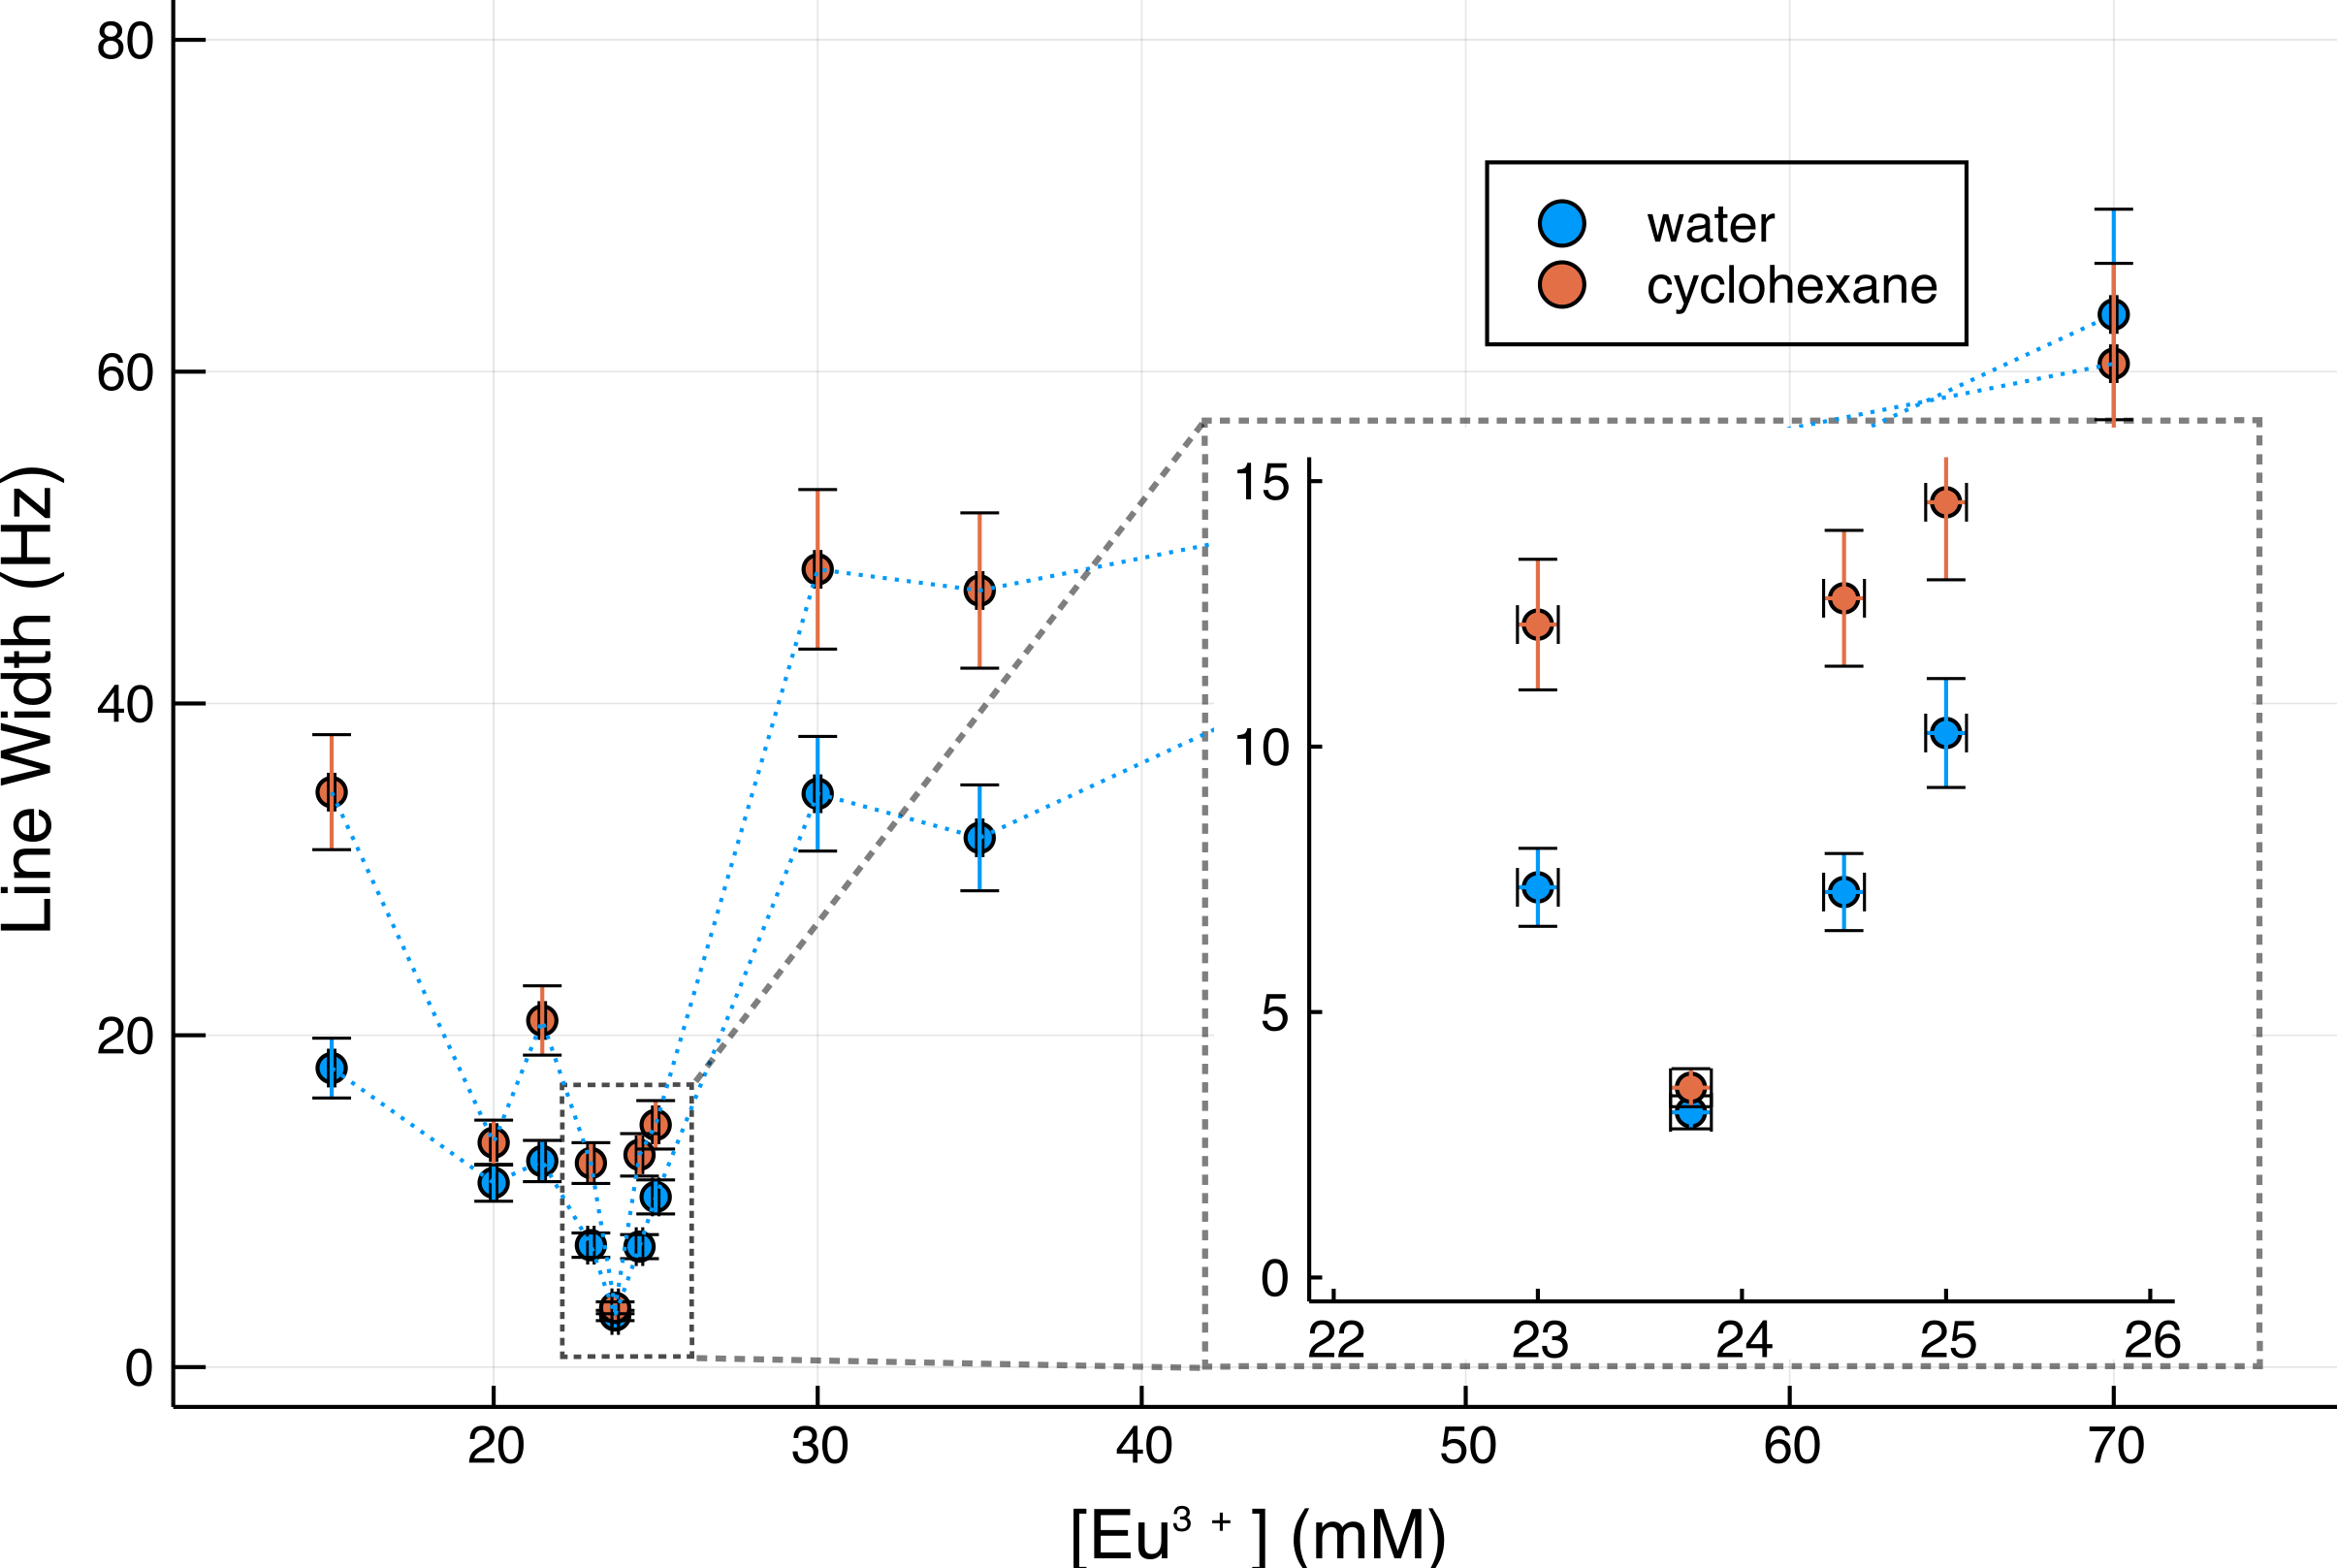
\includegraphics[width=0.8\columnwidth]{mu1y11-dnmr-fi-180618-droplet-lw-mod.png}
  \end{center}
  \caption{Observed line widths of water (blue circles) and
    cyclohexane (orange circles) in microfluidic droplet emulsions
    as a function of the $\ce{Eu[DTPA]^{2-}}$ concentration in the aqueous phase. Inset is the plot around the minimum
    concentration.
    The widths of both lines are minimal
    at the matched concentration of 23.75~mM. }
    \label{fig:linewidths}
\end{figure}


\begin{figure}
  \begin{center}
    \includegraphics[width=1.0\columnwidth]{Field-Maps.pdf}
  \end{center}
  \caption{$B_0$ Field maps obtained by magnetic resonance imaging of emulsions
  with (A) $\Delta\chi=-1.41\times 10^{-6}$ and (B) $\Delta\chi\approx 0$.
  }
  \label{fig:field-map}
\end{figure}




\section{Results and Discussion}


While it is possible to predict the magnetic field distribution in a system of
multiple phases with differing susceptibilities by solving the magnetostatic
equation (\eqn{eqn:Magnetostatic}), this requires precise geometric information on the arragement of the
two phases. In the case of an emulsion, the arrangement of the droplets is not
regular. However, at high droplet densities, it can be
expected to approximate  a dense packing of spheres. In order to obtain a
semi-quantitative prediction, the demagnetising field in
face-centred cubic  (FCC) and simple cubic (SC) lattices of diamagnetic spheres was simulated;
the results are shown in  \fig{fig:FEM-fcc}. A single unit cell containing
one (SC) or
two (FCC) independent spheres was meshed under periodic boundary conditions in all
directions (\fig{fig:FEM-fcc}C).
As is well known, the demagnetising field inside an isolated diamagnetic sphere
is homogeneous, while the field outside of the
sphere is that of a magnetic
point dipole located at the sphere's centre. This situation is approximated
in a lattice if the lattice constant is much larger than the sphere
diameter. The computed demagnetising field
of a small sphere in an SC lattice is shown in \fig{fig:FEM-fcc}A.
The contour levels display the $z$-component of the local demagnetising field
normalised by the background $B_0$ field and the susceptibility difference
$\Delta\chi= \chi_\text{sphere}-\chi_\text{continuous}$. The field is homogeneous
inside the sphere, and a spatially varying demagnetising field only
exists in the continuous phase.
By contrast, in a
densely packed face-centered cubic lattice the field is no
longer homogeneous inside the spheres (\fig{fig:FEM-fcc}B). The FCC
lattice approximates the geometry of a dense microemulsion of homogenous
water-in-oil droplets.  \fig{fig:FEM-fcc}D shows the histograms of
the $z$-components of
the demagnetisig field in the continuous and droplet phases of the FCC
lattice, respectively.

The NMR spectra expected from an ideal emulsion of the same geometry can
be predicted from these histograms
(neglecting no broadening contributions from the sample container).
The magnetic field relevant for nuclear Larmor precession, often referred
to as the "external" field \citep{Levitt:1996tg} $\mathbf{B}_\text{ext}$  from
\eqn{eqn:LarmorSpins} is given by:

\begin{equation}
\mathbf{B}_\text{ext}(\mathbf{r})
= B_0 (1+\frac{\chi_s}{3}) \mathbf{e}_z  - {\mu_0} \nabla U_d(\mathbf{r}),
\end{equation}

where $B_0$ is the magnitude of the external field, $\chi_s$ is the local
magnetic susceptibility, and $U_d(\mathbf{r})$ is the scalar magnetic potential
of the demagnetising field. The volume susceptibility of a solution containing a
paramagnetic species at low concentration $c_p$ is
\begin{equation}
    \chi_s \approx \chi_0 + c_p\,\zeta_P,
\end{equation}
where $\chi_0$ is the volume susceptibility of the pure solvent,
and $\zeta_P$ is the
molar susceptibility of the paramagnetic species. $\zeta_P$ depends
slightly on the molecular environment. For example, values of
$5.86\cdot 10^{-5}\;\mathrm{l/\text{Mol}}$,
$5.68\cdot 10^{-5}\;\mathrm{l/\text{Mol}}$, and
$6.14\cdot 10^{-5}\;\mathrm{l/\text{Mol}}$ have been measured at 300K for
$\ce{Eu_2O_3}$, $\ce{EuF_3}$, and $\ce{EuBO_3}$, respectively\citep{Takikawa:2010iw}
To our knowledge, the precise molar susceptibility of $\ce{Eu[DTPA]^{2-}}$ in
aqueous solution has not been measured to date, but it is likely to be
similar to the above values.

\fig{fig:droplet-spectra} shows $^1$H NMR spectra obtained from emulsions in the chip
shown in \fig{fig:chip-design} with varying $\ce{Eu[DTPA]^{2-}}$ concentrations in the aqueous
phase as indicated in the figure. While the spectra are extremely broad without dopant,
concentrations in the vicinity of 23~mM lead to much sharper lines for both water and cyclohexane,
and the pure phase line widths are recovered at the optimum concentration of $c_p=23.75$~mM.
Using the susceptibilities for $\ce{H2O}$ and cyclohexane given in
Table \ref{tab:suscept}, this leads to molar susceptibility for $\ce{Eu[DTPA]^{2-}}$
of $5.94\cdot 10^{-5}\;\mathrm{l/\text{Mol}}$, well within the range
 of molar susceptibilities reported in literature for other $\ce{Eu^{3+}}$
 compounds. Using this value, the histograms
shown in \fig{fig:FEM-fcc}D can be converted into
predicted emulsion NMR spectra as a function of $\ce{Eu[DTPA]^{2-}}$
concentration in the aqueous phase,
as shown in \fig{fig:predicted-spectra}.
The predicted behaviour is qualitatively similar to the experimental observation; very broad
lines are expected at zero dopant concentration, while sharp lines are recovered near the optimum
concentration. Also, the droplet phase peak is predicted to be narrower than the one from the continuous phase; this is already evident
in the histograms in \fig{fig:FEM-fcc}.  However, the predicted spectra are consistently sharper than the experimentally
observed ones.
It is not entirely clear what causes the discrepancy between the experimental observation
and the simulations. However, it should be noted that the experimental geometry of the emulsion
differs significantly from the simulation; the droplets are neither uniform in size, nor are they
arranged in a crystalline (FCC) lattice.


\begin{figure}
\begin{center}
	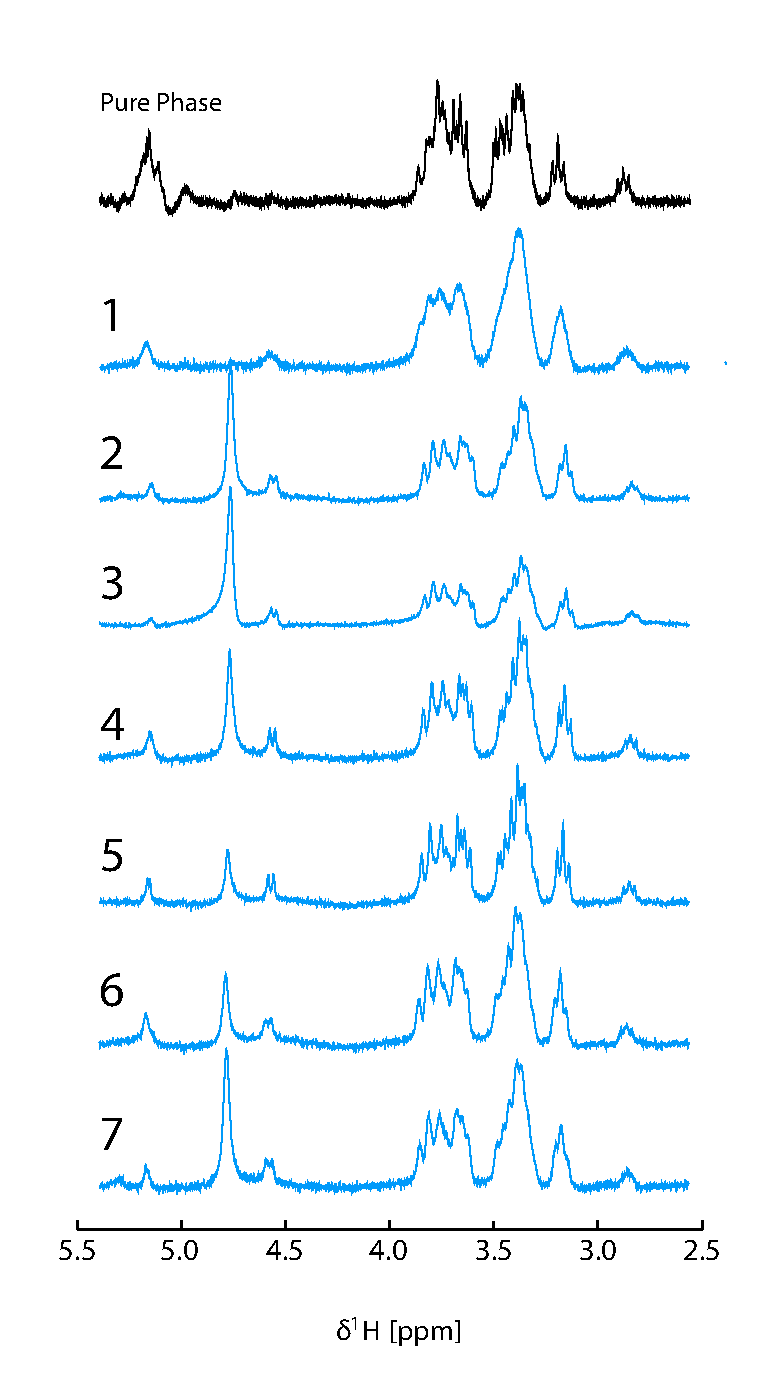
\includegraphics[width=0.7\columnwidth]{wgh2g11-dnmr-fi-180414-001-glucose-wsup}
\end{center}
\caption{Spectra of 200~mM Glucose in $\ce{H_2O}$ obtained from microfluidic droplet emulsions in
	cyclohexane. 1: Aqueous phase contains $c_0=23.75\pm0.25$~mM $\ce{Eu[DTPA]^{2-}}$. Spectra 2-7
	have been obtained by gradual dilution of the aqueous phase with small amounts of DI water.
	2: $\ln c/c0 = -0.5\%$; 3: $\ln c/c0 = -0.75\%$; $4: \ln c/c0 = -0.875\%$;
	$5: \ln c/c0 = -1.0\%$; $6: \ln c/c0 = -1.125\%$; $7: \ln c/c0 = -1.25\%$. A spectrum of pure phase 200mM glucose
	with optimised Eu doping in the same chip is included for comparison (black). The nonuniform peak at 4.8 ppm is due to carrier frequency drift during water suppression }
\label{fig:glucose-dilution}
\end{figure}


The observed widths of the NMR signals from cyclohexane and water
are summarised in \fig{fig:linewidths}. Here, we define the line width as
the ratio of the peak integral to the peak height, multiplied by $2/\pi$. In the
case of Lorentzian line shapes, this definition is equivalent to the full width at half height
(FWHM). However, the expected line shapes from the droplet emulsion are very different
from a Lorentzian (\fig{fig:FEM-fcc}D), such that using the FWHM would be misleading.

Both line widths exhibit a narrow
minimum at 23.75~mM $\ce{Eu[DTPA]^{2-}}$ in the aqueous phase. The water and
cyclohexane minimum peak widths are 3.1~Hz and 3.5~Hz, respectively. For comparison, the best resolution
that has been reached with the same NMR probe is 1.76~Hz for a homogeneous
solution of 150~mM sodium acetate in $\ce{H_2O}$.\citep{Finch:2016gv}

\fig{fig:field-map} shows magnetic field ($B_0$) maps of the sample chambers filled
with droplet emulsions.
In these experiments, two separate
images with different echo times are acquired. The phase difference in each pixel is therefore
proportional to the echo time difference and to the local magnetic field. The echo time difference is constant
therefore the colour denotes the phase acquired by each pixel and can be used to
inform on the homogeneity of the magnetic field in the sample.

In \fig{fig:field-map}A, the droplets do not contain any paramagnetic dopant. As a result, the
susceptibilities of the phases are unmatched, and strong local magnetic field differences
are visible in the images. By contrast, the droplets in \fig{fig:field-map}B are doped with 23.75~mM
$\ce{Eu[DTPA]^{2-}}$. As is clearly visible in the image, the local differences in the magnetic
fields are strongly attenuated in this case.

While the above results have demonstrated that optimal line widths can be minimised in $^1$H NMR
spectra of microfluidic emulsions by paramagnetic doping,
the question remains if this is sufficient to resolve homonuclear
$J$-couplings of a few Hz. This is required in order to do meaningful NMR spectroscopy,
particularly in the context of complex metabolic mixtures.
The top trace in \fig{fig:glucose-dilution} shows a spectrum of 200 mM glucose
and 23.75~mM $\ce{Eu[DTPA]^{2-}}$ in water. The water signal has been suppressed by pre-saturation.
In this case, the resolution is about 3~Hz; such that e.g., the triplet at 3.2~ppm (which corresponds
to the proton in the 2-position on the $\beta$-glucose anomer) is clearly resolved.

Spectrum 1 in \fig{fig:glucose-dilution} has been obtained from
droplet emulsions, starting form an aqueous stock solution prepared to a nominal concentration
of 23.75~mM in $\ce{Eu[DTPA]^{2-}}$ and 200 mM in glucose.
Initially, the resolution in this spectrum is quite poor, in spite of
the attempt to dope at the previously determined optimum concentration. Estimates predicted
the pipetting and weighing errors to add up to an uncertainty in the concentration of the
stock solution of $\pm 1\%$.
Assuming the stock solution was too concentrated, rather than too dilute, it was
then gradually diluted with small amounts of DI water corresponding
to a change in concentration much less than the experimental error in each step.
As can be seen in spectra 2-7, the resolution gradually increases, and matches
the pure phase spectrum at spectrum 5, before it deteriorates again.
In practice, high resolution spectra therefore require careful calibration of the dopant
concentration. It may not be practical to achieve this in one step by preparing the stock
solution, particularly if small volumes are used as in our
experiments. Rather, a gradual dilution as in \fig{fig:glucose-dilution} may be required
to calibrate the $\ce{Eu[DTPA]^{2-}}$ concentration for an accurate match of
the aqueous and carrier fluid susceptibilities. However, if such a match is established,
the resulting resolution is as good as that of the pure aqueous solution.

\section{Conclusion}

Susceptibility differences between the chip,
the aqueous phase, and the oil phase in a microfluidic droplet system can
be successfully mitigated by a combination of structural shimming and
doping of the less diamagnetic of the liquid phases with a europium compound.
The ultimate resolution achieved is only slightly inferior to what has been
demonstrated in homogeneous solutions on a microfluidic chip and is suitable for high
resolution NMR spectroscopy.

%% !TEX root = ./Thesis - combined.tex

\chapter{Parahydrogen induced polarization on a chip} \label{Chapter:Parahydrogen}

 This chapter is an extended version of J Eills\footnotemark, W Hale\footnotemark[\value{footnote}], M Sharma,
 M Rossetto, M H Levitt and M Utz, High-Resolution Nuclear Magnetic Resonance
 Spectroscopy With Picomole Sensitivity by Hyperpolarisation On A Chip,
 \textit{Journal of the American Chemical Society}, 2019 \citep{Hale2019PHIP}
\footnotetext{These authors contributed equally
to the work.}
\section{Synopsis}
In this chapter a device that combines high-resolution NMR and parahydrogen induced hyperpolarization (PHIP)
with a high-sensitivity transmission line micro-detector is discussed.
The para-enriched hydrogen gas is introduced into solution by diffusion
through a membrane integrated into a microfluidic chip.
NMR microdetectors, operating with sample volumes of a few $\mu$l or less,
benefit from a favourable scaling of mass sensitivity discussed
in \ref{Micro-NMR}. However, the small volumes make it very difficult to
detect species present at less
than millimolar concentrations in microfluidic NMR systems.

In view of
overcoming this limitation, parahydrogen-induced polarization
(PHIP) is implemented on a microfluidic device with 2.5~$\mu$l detection volume.
Integrating the hydrogenation reaction into the chip minimises polarization
losses to spin-lattice relaxation, allowing the detection of picomoles of
substance. This corresponds to a concentration limit of detection of better than
1$\mu$M$\sqrt{\text{s}}$, unprecedented at this sample volume.  The
stability and sensitivity of the  system can be used to extract
quantitative information on the hydrogenation kinetics and
their interplay with nuclear relaxation. It is further exemplified by homo-
(\textsuperscript{1}H-\textsuperscript{1}H) and heteronuclear
(\textsuperscript{1}H-\textsuperscript{13}C) 2D NMR experiments
 at natural \textsuperscript{13}C abundance.

 \section{Introduction}

 High-resolution NMR
 spectroscopy is a superbly versatile method which provides detailed, and
 quantitative, information on chemical composition and structure. It is widely
 used to follow the progress of chemical reactions
 \cite{Foley-quantitative:2004bk,Foley:2014kpa},
 as well as
 metabolic processes in living systems
 \cite{Wishart:2008ga,Gottschalk:2008ixa,CuperlovicCulf:2010vc,Shintu:2012bl}.
 However, NMR suffers from inherently low sensitivity
 which is due, in part, to the very weak polarization of nuclear spins along the magnetic
 field for samples in thermal equilibrium at ambient conditions.
 Conventional high-resolution NMR therefore requires nanomole quantities of
 sample. Many important problems require detection of analytes at low
 micromolar concentrations, such as transient reaction intermediates, or
 metabolic species. Despite the
 comparatively higher mass sensitivity of NMR for small sample volumes
 \cite{Olson:1995vu,Bart:2009kc}, conventional micro-NMR systems  around
 1~$\mu$L achieve mass limits of detection of no better than \cite{Finch:2016gv}
 1~nmol$\sqrt{\mathrm{s}}$,  corresponding to a concentration
 limit of detection of 1~$\mathrm{m M \, \sqrt{s}}$. An increase of several
 orders of magnitude in sensitivity is therefore required to enable NMR
 studies of mass-limited samples at micromolar concentrations.

 Microfluidic lab-on-a-chip devices are finding increasing applications in
 chemistry and the
 life sciences. They provide detailed control over the experimental
 conditions at a much smaller length scale than conventional reactors, and
 allow integration of synthesis, separation, and analytical steps on
 a single platform \cite{Wang:2006en,Theberge:2012iq,Hoang:2011du,Ohno:2008da,Zhou:2004id,
 Fang:2018ib,Hoang:2011ee,Gunther:2006vd}. The small size also affords the possibility of
 high experimental throughput.
 In the life sciences, microfluidic devices are increasingly used as
 sophisticated culture platforms for cells,
 cell assemblies, tissues, and small organisms
 \cite{Whitesides:2006vi,
 ElAli:2006ci,West:2008jd,Neuzil:2012gc,Gracz:2015co}.
 The integration of NMR with microfluidics
 \cite{Ryan:2012ke,Badilita:2011td,Spengler:2014ir,Finch:2016gv} is promising, as
 it enables in-situ, non-invasive monitoring of chemical and metabolic processes
 in lab-on-a-chip systems.

 The usefulness of microfluidic NMR could be significantly
 enhanced if the following conditions could be met:
 (i) sample volumes around 1~$\mu$l or less;
 (ii) a concentration limit of
 detection near  1~$\mu$M$\sqrt{s}$; and
 (iii)  spectral
 resolution of better than 0.01~ppm to allow distinction and identification
 of chemical species.

 Although exquisitely sensitive NMR detection schemes exist,
 approaching even single-spin detection in favourable cases
 \cite{Rugar:1992dm,Rugar:2004bc,Mamin:2007ff,Poggio:2010jf,
 Maze:2008cs,Staudacher:2013kn,Rugar:2015by,McDermott:2002hp,
 Budker:2007hz,Xu:2006kg,Blanchard:2013gs}, they lack spectral resolution.
 While a recent study
 has demonstrated resolution of $J$ couplings using a nitrogen-vacancy
 (NV) centre magnetometer \cite{Glenn:2018ct}. None of these
 alternative detection schemes are compatible with high (several Tesla)
 magnetic fields, which are essential to produce spectral dispersion
 by chemical shifts.
 So far, no method has been demonstrated with the combination of high
 spectral resolution, high chemical dispersion,
 and high sensitivity for small volumes required for
 advanced microfluidic NMR measurements significantly
 below the 1~mM concentration scale.

 Hyperpolarization methods generate substances which exhibit a transiently high
 level of nuclear spin polarization, with an increase in the NMR signal strength
 of more than 4 orders of magnitude \cite{munnemann2011nuclear}, and can be combined
 with micro-NMR detectors and microfluidic systems \cite{McDonnell:2005dn,Desvaux:2009bq,Telkki:2010vg,Paciok:2011e,
 JimenezMartinez:2014et,Causier:2015fg,eills-hale2018EuromarPHIP,Bordonali:2019jqa}.
 One such method
 involves the chemical reaction of the singlet spin isomer of molecular
 hydrogen, and is called parahydrogen-induced hyperpolarization (PHIP)
 \cite{hovener2018parahydrogen,duckett2012application,gloggler2013hydrogen,green2012theory}.

 While most studies have so far brought the reaction liquid in direct contact
 with hydrogen gas either through bubbling or by atomisation of the liquid
 in a hydrogen-filled chamber \cite{bhattacharya2007towards,chekmenev2008pasadena,
 chekmenev2009hyperpolarized,shchepin2014parahydrogen,
 Reineri:2015he,cavallari201813,eills2017singlet},
 liquid-gas interfaces and in particular bubbles
 pose difficulties in the context of microfluidic devices, since they tend
 to alter the flow properties, and can block fluid transport altogether.
 Continuous delivery of parahydrogen by diffusion through
 gas-permeable membranes has been demonstrated at
 conventional size scales \cite{Roth:2010hk,Lehmkuhl:2018cd}.
 It has been shown that silicone elastomer membranes can be used
 to deliver parahydrogen directly to a flowing liquid in a microfluidic
 device \cite{eills-hale2018EuromarPHIP}. Bordonali et al \cite{Bordonali:2019jqa} have
 recently combined a microfluidic NMR probe system with a gas exchange
 chip based on a silicone elastomer membrane to implement the SABRE (signal
 enhancement by reversible exchange) variant of parahydrogen-induced polarization,
 but achieved only small signal enhancement factors (3 to 4).

 In distinction from previous work
 \cite{bhattacharya2007towards,chekmenev2008pasadena,
 chekmenev2009hyperpolarized,shchepin2014parahydrogen,
 Reineri:2015he,cavallari201813,eills2017singlet,Lehmkuhl:2018cd},
 this work integrates the hydrogenation reactor into the chip itself, which greatly
 reduces the polarization losses due to spin-lattice relaxation.
 As shown below, a signal enhancement factor over thermal polarization
 of about 1800 is achieved, allowing detection of a
 picomole quantity of analyte in a sample volume of 2.5 $\mu$l,
 while maintaining the full resolution of conventional $\ce{^1H}$
 NMR spectroscopy.

 This is accomplished by letting the parahydrogen gas diffuse through a
 silicone elastomer membrane \cite{Lehmkuhl:2018cd}
 to come into contact with a solution
 flowing through the chip at a constant rate. The solution
 contains a precursor, which is hydrogenated through a homogeneous
 catalyst also present in the solution. Two hydrogenitive PHIP experiments are performed in
 this way. In the ALTADENA experiment, the solution is hydrogenated 'on-chip' at low magnetic field
 and transferred to a high field magnet for detection. ALTADENA is used as a proof of principle that the device
 is capable of hydrogenation 'on-chip'. In the PASADENA reactions,
 the microfluidic device is held in the bore of a conventional
 NMR magnet using a purpose-built transmission line NMR probe.
 This yields a continuous on-chip stream of hyperpolarized material. As shown
 in the following, in addition to very high detection
 sensitivities, this also results in a continuous and highly stable operation
 of the system, making it possible to perform hyperpolarized
 two-dimensional NMR experiments \cite{Roth:2010hk,Giraudeau:2009fn,Lloyd:2012cf,Eshuis:2015ce}.
 By replacing the hyperpolarized gas feed with hydrogen gas at thermal
 equilibrium, it is possible to gain kinetic information on the hydrogenation
 process, as well as to calibrate the intensity of the hyperpolarized NMR signals.
 This allows accurate assessment of the achieved polarization levels, something
 that has been notoriously difficult in the context of
 parahydrogen-induced polarization.

 \section{Hyperpolarization}


 \subsection{Sensitivity}\label{Sensitivity}

As described in \ref{EnergyLevels}, NMR has low polarization levels that are governed by the Boltzmann
distribution given in \eqn{eqn:Polarization}. For example, for a spin-1/2 particle in a static field of 14.1 Tesla
there is only a factor of $~6\times10^{-6}$ difference in the populations of the $\ket{\alpha}$ and $\ket{\beta}$ state.
Compared to other detection techniques, NMR suffers from poor limits of detection (LODs)
in comparison to other detection methods. Raman Spectroscopy, has
LODs of $10^{-12} - 10^{-15}$ M, Laser induced fluorescence (LIF) has detected concentrations at $10^{-13}$ M and
mass spectrometry has achieved $10^{-19}$ M. These alternative techniques are several orders of magnitude higher than that of NMR.
While sensitivity is not a strong point, NMR is quantitative, non-invasive, and non-destructive making it an ideal
tool for mass limited and, in particular, living samples.

\subsection{Hyperpolarization}

 From \eqn{eqn:Polarization} in \ref{EnergyLevels}, it is found that, the polarization level of nuclear spins at room temperature is low. In fact,
 for protons, it is only $3\times10^{-6}$ per Tesla \citep{RN138}. The signal derived from an NMR experiment
 is proportional to this polarization and means that the sensitivity and LOD is limited. The highest
 field available commercially is ~28 Tesla which corresponds to polarization levels in protons of ~$10^{-4}$ and
 whilst there are clear advantages to working in higher fields the size and more importantly - cost, make them
 unsuitable for many applications. Clearly just increasing the field is not a viable
 option if close to unity polarization is to be
 achieved.

 There are techniques for increasing the spin polarization levels in samples to beyond the thermal
 equilibrium. The general term used to describe these is hyperpolarization. Hyperpolarization has
 applications in a diverse range of fields such as MRI \citep{RN139,RN140,RN151,RN152}, drug discovery
 \citep{RN141,RN142}, reaction monitoring \citep{RN143,RN144,RN145}, metabolomics \citep{RN147,RN148},
 catalysis\citep{RN149, RN150} and material chemistry \citep{RN153,piveteau2015structure,RN154}.

 However, these hyperpolarized states are still subject to relaxation as discussed in \ref{Relaxation} and
 return to thermal equilibrium with time constant $T_1$. This means the hyperpolarized spin order lasts seconds
 to minutes which limits their applications.

 \subsection{Techniques}

 \subsubsection{Brute Force}

 The most simple technique for hyperpolarization is "brute force". It is performed by simply
 cooling the sample to a few degrees kelvin in a high magnetic field \citep{RN155,RN157}, under
 these circumstances, the polarization of $^1$H nuclei is \~$1\%$. In an experiment, the sample
 is first cooled to \~2.3 K, after which, there is a waiting period to allow for the build up of polarization
 of the $^1$H nuclei. This period is required due to long $T_1$ times at cryogenic temperatures and
 can be up to 70 hours \citep{RN155}. After the polarization build up, the solid sample is passed
 through a low field to facilitate thermal mixing and polarizaiton of $^{13}$C nuclei. Finally,
 the solid sample is rapidly dissolved in warm solvent and detected.

 There are drawbacks however, firstly, the long $T_1$ times at cryogenic temperatures mean long
 wait times are required in order to sufficiently build up polarization in the sample and prohibit high-throughput production.
 Secondly, and perhaps more importantly, the limit of polarization with this technique is around $10^{-2}$ at achievable
 magnetic fields and temperatures.

 \subsubsection{Dynamic Nuclear polarization}

Dynamic nuclear polarization (DNP) methods use the thermal equilibrium electron spin polarization to polarize the nuclei under investigation. Close to unity
polarization of the electrons is achieved by cooling to cryogenic temperatures (<2K) in a high magnetic field (>7 T).
The electron polarization is transferred to nearby nuclear spins by saturating one of the transistions of the electron-nuclear
coupled spin system with microwave frequency radiation.

The source of the electrons are 'free radicals' - molecules that have an unpaired electron spin, that
are spread homogeneously throughout the sample. After cooling, the sample is held in a cryostat which is at
1.2 - 1.5K. The electrons have a much shorter $T_1$ in contrast to nuclear spins so after irradiation with
microwave radiation to induce polarization transfer between electrons and nuclei, the electrons repolarize
quickly compared to the nuclei who retain non-equilibrium polarization. This polarization diffuses throughout the
sample. After some time, tens of minutes is not uncommon, the nuclear spins are polarised to around 0.1 or 10\%. The
sample is then detected, either as the solid, or a liquid, depending on which type of DNP is being performed.

Several different types of DNP have been reported. These are solution
state DNP \citep{RN158}, solid state magic angle spinning (MAS) DNP \citep{RN159}, rapid-melt DNP \citep{sharma2015rapid} and static solid state DNP with
dissolution and observation \citep{RN160}. The latter is most commonly referred to as dissolution-DNP and written as d-DNP.

The large equipment required for d-DNP, as well as the high cost of liquid helium for the cryostat and
the extra superconducting magnet can make this method prohibitive for most NMR groups.

 \section{Parahydrogen Induced polarization - PHIP}

 \subsection{Parahydrogen}

 Hydrogen exists as a diatomic made up of two protons and two electrons. As such, the total
 wave function contains electronic, vibrational, rotational and spin components and can be
 written as:

 \begin{equation}
  \Psi^{tot} =\Psi^{elec}\Psi^{vib}\Psi^{rot}\Psi^{spin}
 \end{equation}

 Because the two protons are fermions they are subject to the Pauli exclusion principle
 which states that the total wave function must be antisymmetric with respect to exchange. With
 this is mind, it is important to note that the electronic, and vibrational states, are symmetrical
 in the ground state.  and it is assumed that they occupy the ground state, the symmetry
 of the overall wave function therefore depends of the symmetry of $\Psi^{rot}$$\Psi^{spin}$.

 Rotational wavefunctions have quantum number $J$. For even numbers of $J$ ($J$=0,2...) the wavefunction
 is symmetric with respect to particle exchange for odd numbers of $J$ ($J$=1,3...) the wavefunction is
 antisymmetric. The nuclear spin wave function can also be symmetric or antisymmetric. By adding the
 angular momentum of both spins, it can be shown that they combine to give four possible quantum states
 with column vector representations derived from \eqn{eqn:2spinstates}:

 \begin{align}\label{eqn:H2states}
 \ket{T^+} =& \ket{\alpha\alpha} = \begin{pmatrix}
   1\\
   0\\
   0\\
   0
 \end{pmatrix}\\
 \ket{T^0} =& \frac{1}{\sqrt{2}}\ket{\alpha\beta}+\ket{\beta\alpha} = \frac{1}{\sqrt{2}}\begin{pmatrix}
   0\\
   1\\
   1\\
   0
 \end{pmatrix} \\
 \ket{T^-} =& \ket{\beta\beta} = \begin{pmatrix}
   0\\
   0\\
   0\\
   1
 \end{pmatrix}\\
 \ket{S^0} =& \frac{1}{\sqrt{2}}\ket{\alpha\beta}-\ket{\beta\alpha} = \frac{1}{\sqrt{2}}\begin{pmatrix}
   0\\
   1\\
   -1\\
   0
 \end{pmatrix}.
 \end{align}

 The three triplet ($T$) states have spin quantum number $I$ = 1 and $m_I$ = +1, 0, and -1 denoted by the superscript symbol on each state.
 The singlet ($S$) state has $I$ = 0 and $m_I$ = 0. The triplets states are symmetric with respect to spin exchange, whilst the
 singlet state is anti-symmetric with respect to spin exchange. Hydrogen in the triplet state is referred to as \textit{ortho} and the
 singlet state is referred to as \textit{para}.

 In order for $\Psi^{tot}$ to be antisymmetric, the antisymmetric rotational states are restricted to coupling to the symmetric
 (triplet) spin states whilst the symmetric rotational states are restricted to coupling to the antisymmetric (singlet) state.

 The rotational energy is given by $E_j = \frac{J(J+1)\hbar^2}{2I}$
 where $I$ is the moment of inertia of the diatomic and is given by $I = \mu l^2$, where $\mu$ is the reduced mass,
 and $l$ is the internuclear distance.

 \begin{figure*}
   \begin{center}
   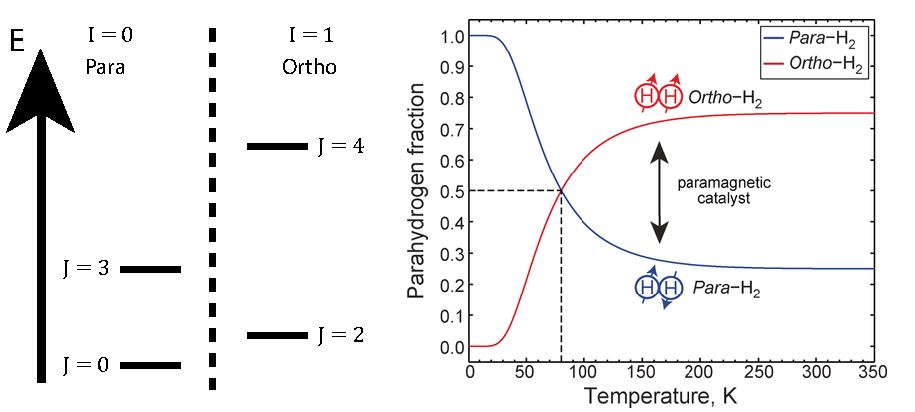
\includegraphics[width=\textwidth]{Para-OrthoH2.pdf}
   \end{center}
   \caption{Left: The rotational energy levels of para- and orthohydrogen with their associated J values. Right: a graph
   showing the fraction of para- and orthohydrogen as a function of temperature. The dotted line shows 50\% para
   enrichment that is achieved by cooling to 77K using liquid nitrogen. Image taken from \citep{barskiy2017nmr}.}
   \label{fig:POH2}
 \end{figure*}


 At room temperature, the ratio of \textit{ortho} to \textit{para} hydrogen is very nearly 3 to 1. However, by cooling down hydrogen
 the lowest ($J$ = 0, 1) rotational energy states start to become populated. The ratio of \textit{para} to \textit{ortho} hydrogen may be
 calculated using the respective partion functions \citep{GREEN20121}:
\begin{equation}
  \frac{N_{\text{para}}}{N_{\text{ortho}}} = \frac{\sum_{J = \text{even}}(2J+1)\text{exp}\{-\frac{J(J+1)\theta_R}{T}\}}{3\sum_{J = \text{odd}}(2J+1)\text{exp}\{-\frac{J(J+1)\theta_R}{T}\}},
\end{equation}
for the first few levels this is:
\begin{equation}\label{eqn:partition}
  \frac{N_{\text{para}}}{N_{\text{ortho}}} = \frac{1 + 5\text{exp}\{-\frac{6\theta_R}{T}\} + 9\text{exp}\{-\frac{20\theta_R}{T}\} + 13\text{exp}\{-\frac{42\theta_R}{T}\} + \dots}{3(3\text{exp}\{-\frac{2\theta_R}{T}\} + 7\text{exp}\{-\frac{12\theta_R}{T}\} + 11\text{exp}\{-\frac{30\theta_R}{T}\} + \dots)},
\end{equation}
 where the rotational constant, $\theta_R$, is:
 \begin{equation}
   \theta_R = \frac{h^2}{8\pi^2Ik_b}.
 \end{equation}

Using \eqn{eqn:partition}, the percentage of parahydrogen in an equilibrium mixture can be plotted as a function of temperature, shown in \fig{fig:ParaTemp}.

\begin{figure}[ht]
  \begin{center}
  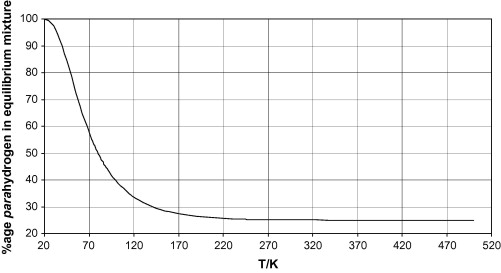
\includegraphics{ParaTemp-dependance.jpg}
  \end{center}
  \caption{Calculated percentage of parahydrogen in an equilibrium mixture of \textit{ortho}- and \textit{para}hydrogen gas
  as a function of temperature using \eqn{eqn:partition} and $\theta_R$ = 87.6 K. Taken from \citep{GREEN20121}.}
  \label{fig:ParaTemp}
\end{figure}

 By cooling alone, the ratio would remain unchanged, conversion
 from ortho to para spin states without the aid of a catalyst (typically charcoal or iron (III) oxide) is not possible.
 The catalyst temporarily breaks the symmetry of the \ce{H_2} molecule which allows spin-spin transitions and leads to
 a much larger fraction of the \textit{para} form of hydrogen. Crucially, when warmed up to
 room temperature in the absence of a symmetry breaking catalyst, no conversion from the singlet state $\ket{S^0}$ back to
 the triplet states $\ket{T^+}$, $\ket{T^0}$, $\ket{T^-}$ occurs. This is because transitions between singlet and triplet states
 are forbidden through quantum mechanical selection rules. It is therefore possible to store pure parahydrogen
 in the right container for days to weeks.

 Para enrichment fraction, $f$, can be measured by NMR. By measuring the o\ce{H_2} signal of the enriched \ce{H_2} ($S_{e}$)
 and comparing it to the signal obtained from the same amount of \ce{H_2} at room temperature ($S_{rt}$).
 The enrichment fraction is given by \citep{RN131, RN132}:

 \begin{equation}\label{pfrac}
   f = 1 -(3S_{e}/4S_{rt})
 \end{equation}

 \subsection{PASADENA and ALTADENA}\label{PASADENA and ALTADENA}

 'Parahydrogen and synthesis allow dramatically enhanced nuclear alignment'
 (PASADENA)\citep{RN129} and 'adiabatic longitudinal
 transport after dissociation engenders net alignment' (ALTADENA)\citep{RN128}
 are subclasses of PHIP experiments characterised by the strength of magnetic
 field in which the hydrogenation and detection are performed.

 The difference between PASADENA and ALTADENA are the $J$-coupling regimes in which the reaction and detection happens.
 The regime is determined by the value of the $J$-coupling (in Hz) compared to the value of the difference in chemical
 shifts of the individual protons. Where the strong regime has J-couplings that take the approximate value of the difference in chemical shift
 ($\frac{\delta{\omega}}{J}\approx1$), and the weak regime has J-couplings much smaller than the difference in chemical
 shift ($\frac{\delta{\omega}}{J}>>1$). Since the chemical shift depends on external magnetic field ($B_{0}$) and the
 J-couplings are independent of field one can select an appropriate magnetic field for the desired experiment.
 In PASADENA experiments the reaction and detection is carried out at high field (>1 T) whereas in
 ALTADENA the reaction is carried out at low field (< 10 mT), and the product is transferred to a high magnetic field for detection\citep{RN130}.

This difference manifests itself as a difference in $J$-coupling regimes in the
\textit{para}hydrogen derived hydrogens in the product molecule. ALTADENA
refers to hydrogens in the strong coupling regime upon addition and PASADENA
refers to the weak coupling regime upon addition.


 \subsubsection{Spin Physics}

 The spin physics of PASADENA and ALTADENA can be interpreted through the density operator formulism. In a
 PASADENA type experiment, parahydrogen is added to a molecule in high field forming a weakly coupled AX
 system of the type discussed in \ref{PASADENA and ALTADENA}. Due to the weak coupling, $\frac{\delta{\omega}}{J}>>1$, the eigenbasis is close to the
 Zeeman basis. The initial density operator, $\hat{\rho}_{\text{ini}}$, can be defined using
 \eqn{eqn:H2states} as:
 \begin{equation}
   \hat{\rho}_{\text{ini}} = \ket{S^0}\bra{S^0} = \frac{1}{2}\ket{\alpha\beta -
   \beta\alpha}\bra{\alpha\beta - \beta\alpha},
 \end{equation}
 using the zeeman basis states for a 2 spins system from \eqn{eqn:H2states} the
 matrix representation is:
 \begin{align}
   \hat{\rho}_{\text{ini}}\quad=& \frac{1}{2} \begin{pmatrix}
   0\\
   1\\
   -1\\
   0
   \end{pmatrix} \otimes \begin{pmatrix}
     0 & 1 & -1 & 0
     \end{pmatrix}\\
   =& \frac{1}{2}\begin{pmatrix}
   0 & 0 & 0 & 0\\
   0 & 1 & -1 & 0\\
   0 & -1 & 1 & 0\\
   0 & 0 & 0 & 0
 \end{pmatrix}.
 \end{align}

This density operator may also be expressed as a linear combination of operators:
\begin{equation}
  \rho_{\text{ini}} = \frac{1}{4}\mathbb{1} - (\hat{I}_{1x}\hat{I}_{2x} + \hat{I}_{1y}\hat{I}_{2y} + \hat{I}_{1z}\hat{I}_{2z}).
\end{equation}

 These diagonal elements (populations) do not evolve as these components commute with the Hamiltonian. The off-diagonal
 elements (coherences) evolve at a rate $\approx\delta{\omega}$.

The Hamiltonian of the product molecule is given by:
\begin{equation}
  \hat{H}_{\text{pas}} = 2\pi(\omega_1\hat{I}_{1z}) + 2\pi(\omega_2\hat{I}_{2z}) + 2\pi~J_{12}(\hat{I}_{1x}\hat{I}_{2x} + \hat{I}_{1y}\hat{I}_{2y} + \hat{I}_{1z}\hat{I}_{2z}),
\end{equation}
 as the reaction continues, an ensemble of molecules are hydrogenated at different time points, this gives
 a new density operator, $\hat{\rho}_{pas}(t)$, expressed as:
 \begin{equation}
   \hat{\rho}_{\text{pas}}(t) = \text{exp}\{-i\hat{H}_{\text{pas}}t\}\hat{\rho}_{\text{ini}}\text{exp}\{+i\hat{H}_{\text{pas}}t\}.
 \end{equation}

Usually, the hydrogenation period is much longer than the coherence evolution. A new average density operator
can be found by averaging the ensemble over the reaction time, $t_r$ by:
\begin{equation}
  \overbar{\hat{\rho}}_{\text{pas}}(t_r) = \frac{1}{t_r}\int_{t=0}^{t_r}\hat{\rho}_{\text{pas}}(t)dt,
\end{equation}
these coherences average to zero over the reaction time period and so the
 density operator becomes:
 \begin{equation}
   \hat{\rho}_{\text{pas}} = \frac{1}{2}\begin{pmatrix}
   0 & 0 & 0 & 0\\
   0 & 1 & 0 & 0\\
   0 & 0 & 1 & 0\\
   0 & 0 & 0 & 0
 \end{pmatrix},
 \end{equation}
and can also be written as:
\begin{equation}
   \hat{\rho}_{\text{pas}}(t_r) = \frac{1}{4}\mathbb{1} - \hat{I}_{1z}\hat{I}_{2z},
\end{equation}
 \fig{fig:PASADENA} shows the eigenstate populations and general simulated spectra of a thermal equilibrium experiment and
 a PASADENA experiment.

 In a usual NMR spectrum, a $\pi/2$ pulse is used to excite observable single quantum coherences. For a PASADENA signal to
 be observed, a $\frac{\pi}{4}$ pulse must be used. The reason becomes clear when examining the effect on $\hat{\rho}_{\text{pas}}(t_r)$ of a pulse with general
 tilt angle, $\theta$, along the $y$-axis:
\begin{equation}
  \hat{R}(\theta)_y\hat{\rho}_{\text{pas}}(t_r) = \hat{\rho}_\theta~p = \cos^2(\theta)\hat{I}_{1z}\hat{I}_{2z} +
  \cos(\theta)\sin{\theta}(\hat{I}_{1z}\hat{I}_{2x} + \hat{I}_{1x}\hat{I}_{2z}) + \sin^2(\theta)\hat{I}_{1x}\hat{I}_{2x},
\end{equation}
using a tilt angle of $\theta = \pi/2$ would give:
\begin{equation}
  \hat{\rho}_{\pi/2p}  = \hat{I}_{1x}\hat{I}_{2x},
\end{equation}
which is unobservable double quantum coherence. However, a pulse with $\theta = \pi/4$ gives:
\begin{equation}
  \hat{\rho}_{\pi/4p} = \frac{1}{2}(\hat{I}_{1z}\hat{I}_{2z} + \hat{I}_{1z}\hat{I}_{2x} + \hat{I}_{1x}\hat{I}_{2z} + \hat{I}_{1x}\hat{I}_{2x}),
\end{equation}
where the $\hat{I}_{1x}\hat{I}_{2z}$ and $\hat{I}_{1z}\hat{I}_{2x}$ terms are observable.

 \begin{figure*}[ht]
   \begin{center}
   \includegraphics[width=\columnwidth]{Pasadena-population-Balls.pdf}
   \end{center}
   \caption{Above: Populations of states represented as balls in a thermal (left) and a PASADENA experiment. Below: Simulations
   of spectra arising from adding thermal hydrogen to a molecule (left) and of a PASADENA experiment when adding parahydrogen.}
   \label{fig:PASADENA}
 \end{figure*}

 In an ALTADENA experiment, the hydrogenation is performed at low field. In this case, when a molecule of hydrogen
 is added to a substrate the density operator, $\hat{\rho}_\text{ini}$, is projected onto the new eigenbasis which
 at low field (where $\frac{\delta{\omega}}{J}<<1$) is the singlet-triplet basis. To a good approximation the only term
 is the $\ket{S_0}$ and there is no evolution of the system.

 The sample is then transferred to high-field (where $\frac{\delta{\omega}}{J}>>1$). It is done adiabatically, this means that the rate
 of change of magnetic field, $dB_0/dt$ being small with respect to the value of the $J$-coupling between the protons, squared i.e. $dB_0/dt < (J_{12})^2$. As
 the field increases, the eigenbasis changes from singlet-triplet to the Zeeman basis. The adiabatic change carries the population of the
 $\ket{S_0}$ state to the $\ket{\alpha\beta}$ or $\ket{\beta\alpha}$ state, depending on which is more energetically more favourable.
 This change is depicted graphically in \fig{fig:SingletTriplet} where $\ket{\beta\alpha}$ has been arbitrarily chosen as the lower energy state.
 In the case shown, only one of the four energy levels, namely $\ket{\beta\alpha}$ is now populated, therefore the density operator, $\hat{\rho}_{alta}$ is given by:
 \begin{equation}
   \hat{\rho}_{\text{alta}} = \ket{\beta\alpha}\bra{\beta\alpha}.
 \end{equation}
  This leads to \citep{RN128}:
 \begin{equation}
   \hat{\rho}_{\text{alta}} = \hat{I}_{1z}\hat{I}_{2z}±\frac{1}{2}(\hat{I}_{1z}-\hat{I}_{2z}),
 \end{equation}
 where the positive sign applies if $J_{12}(\omega_1 - \omega_2)<0$, and the negative
 sign applies in the opposite case.

 \begin{figure}
   \begin{center}
   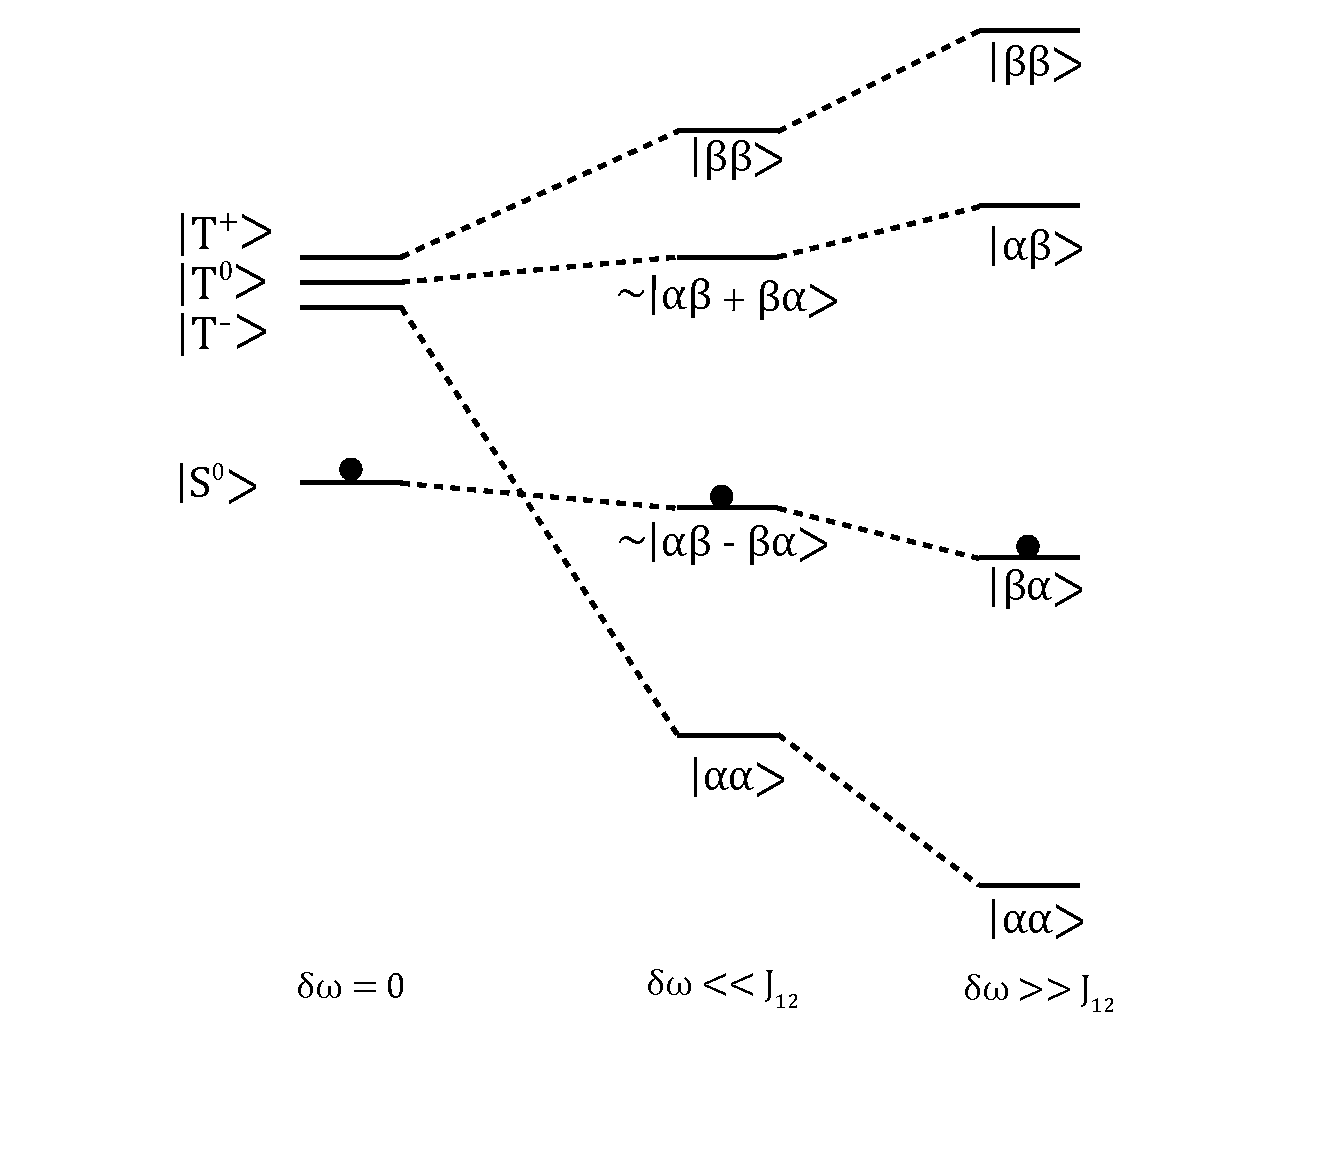
\includegraphics[width=\columnwidth]{ALTADENA-overview.pdf}
   \end{center}
   \caption{Correlation diagram for the ALTADENA effect. Hydrogenation at low field populates the singlet state, adiabatically increasing
   the field carries the population into a high field state.}
   \label{fig:SingletTriplet}
 \end{figure}

 An r.f. pulse with general angle, $\theta$, orientated along the $y$-axis gives:
 \begin{equation}
   \hat{R}(\theta)_y\hat{\rho}_{\text{alta}} = \hat{\rho}_\theta = \cos(\theta)\sin{\theta}(\hat{I}_{1z}\hat{I}_{2x} + \hat{I}_{1x}\hat{I}_{2z})
   ± \frac{1}{2}\sin\theta(\hat{I}_{1x} - \hat{I}_{2x}).
 \end{equation}
 A pulse with $\theta = \pi/4$ here yields:
 \begin{equation}
   \hat{\rho}_{\pi/4a} = \frac{1}{2}(\hat{I}_{1z}\hat{I}_{2x} + \hat{I}_{1x}\hat{I}_{2z}) ± \frac{1}{2\sqrt{2}}(\hat{I}_{1x} - \hat{I}_{2x}),
 \end{equation}
 that gives rise to two out of phase doublets shown in \fig{fig:ALTADENA}.
 However, unlike PASADENA, ALTADENA does not require
 a $\pi/4$ pulse so $\pi/2$ pulses are more common.

 \begin{figure}
   \begin{center}
   \includegraphics[width=\columnwidth]{Altadena-Population-Balls.pdf}
   \end{center}
   \caption{Top: Populations of Zeeman states represented by balls for thermal(left) and ALTADENA(right) experiments.
   Bottom: Simulations of a thermal spectrum after applying a $\pi/4$ pulse and an ALTADENA experiment.}
   \label{fig:ALTADENA}
 \end{figure}

\newpage

\section{Materials and methods}\label{pHMaterialandMethods}

The microfluidic chips for the PASADENA experiments were constructed from three layers of cell cast PMMA sheet
material (Weatherall Equipment). The sheet thickness was 200 $\mu$m for the
top and bottom layers, and 500 $\mu$m for the middle layer. The fluid and gas
channels were designed on AutoCAD and cut into the PMMA using a laser cutter
(HPC Laser L3040) to a width and depth of 150 $\mu$m. The layers were
subsequently bonded together with a plasticiser (2.5\% v/v dibutyl phthalate in
isopropyl alcohol) under heat and pressure (358 K, 3.5
tonnes) \cite{Yilmaz:2016fx}. The total internal fluid volume is 4~$\mu$l, and
the sample chamber is 2.5~$\mu$l.

The chip for the ALTADENA experiment was a single 500 $\mu$m layer of
PMMA. The fluid and gas channels for this device were designed and cut in
the same manner as above.

Both devices also employ a poly(dimethyl siloxane) (PDMS) membrane
(Shielding Solutions) to facilitate para-H\textsubscript{2} transport,
of 1 mm thickness with laser-cut screw holes. The parahydrogen
polarization lifetime in the PDMS after O\textsubscript{2} removal was
measured to be \textasciitilde{}4 h.

The PMMA chips and PDMS membrane layer are sealed with a pair of
screw-tightened 3D printed (Accura Xtreme, Proto Labs) holders, with
fluid and gas in/out ports (to fit Kinesis UK NanoPorts).

For PASASDENA experiments, the assembled microfluidic device was put in a transmission line based
home-built probe \cite{sharma2019modular}. The
device sits between the two stripline planes on a sample holder having
sample chamber of the device coinciding with the constriction on
stripline planes. PASADENA and 2D NMR experiments were performed at a field strength
of 11.7~T with an AVANCE III console. Nutation frequencies for RF pulses
were 100~kHz for protons, and 20~kHz for carbon in the case of the HMQC
spectrum. 16k data points were acquired over 1.2~s for proton 1D spectra.
Saturation recovery experiments used a train of 512 $\pi/2$ pulses
separated by a delay of 0.1~ms, followed by a recovery delay, and a $pi/4$
excitation pulse.
The PH-TOCSY spectrum was acquired using the States-TPPI method,
with 256 $t_1$ increments, averaging 8 transients per increment.
2048 complex data points in 0.2~s were acquired for each increment.
The PH-HMQC experiment was acquired using the States method, with
128 $t_1$ increments, averaging 8 transients with 2048 complex points
over 0.2~s. 1D spectra and
2D spectra were processed using scripts written in Julia \cite{Bezanson:2017gd}.

For ALTADENA experiments, the device was placed outside the magnet in order
for the hydrogenation to occur at low field. The solution was passed through the
device and into a 5 mm NMR tube (NORELL). ALTADENA NMR experiments were performed at
a field strength of 16.5 T with a NEO console with cryoprobe. The 1D spectra
were processed also using scripts written in Julia \cite{Bezanson:2017gd}.

To generate parahydrogen gas at 50\% para enrichment, hydrogen gas
(purity 99.995\%) was passed through a home-built parahydrogen generator
containing an iron (III) oxide catalyst cooled to 77~K using liquid
nitrogen.

The solution before both experiments contained 20 mM propargyl acetate \textbf{2}
and 5 mM
1,4-bis(diphenyl\-phosphino)\-butane(1,5-cyclo\-octadiene)\-rhodium
tetra\-fluoro\-borate \textbf{3} in methanol-d\textsubscript{4}. In an attempt to
avoid possible spin relaxation or chemical side-reaction effects,
dissolved oxygen from the atmosphere was removed by 5 minutes of
vigorous helium bubbling.

The parahydrogen gas was delivered through a PTFE tube (1/16 inch O.D.,
1/32 inch I.D.) into the 3D printed chip holder, and out via a second
PTFE line, using a mass flow controller (Cole-Parmer) to limit the flow
to 20 ml min\textsuperscript{-1} at an overpressure of 5 bar. Although
most of the parahydrogen gas passes directly through the system, some
amount dissolves into the PDMS layer, which in terms of
H\textsubscript{2} solubility behaves similarly to other organic
solvents. The solution was loaded into a 3.5 ml plastic syringe with a
Luer lock connection to in-flow PEEK tubing (1/16 inch O.D., 0.007 inch
I.D.) leading to the chip. The same tubing was used for the solution
out-flow into a container exposed to a back pressure of 1.5 bar of
nitrogen gas, to preventing formation of hydrogen bubbles in the chip.
Solution flow into the chip was controlled with a syringe pump (Cole-Parmer).

\section{Results and Discussion}

\subsection{Parahydrogen relaxation in PDMS}

To determine the hydrogen ortho-para
conversion in PDMS, the ortho-para conversion time of H2 dissolved in PDMS
was measured. A high-pressure NMR tube of 5 mm outer diameter
(Sigma-Aldrich) was filled with PDMS resin (Sylgard 84, 3M). A teflon
capillary of 1/16 inch outer diameter (Sigma-Aldrich) was pushed
into the NMR tube along the central axis, and the PDMS was allowed to cure.
The capillary was then removed, leaving a cylidrical void in the centre of
the NMR tube. The tube was then exposed to vacuum for varying amounts of
time, in order to study the conversion effect of the residual oxygen the
results of which are shown in \fig{fig:ph2conv}.

\begin{figure}[ht]
  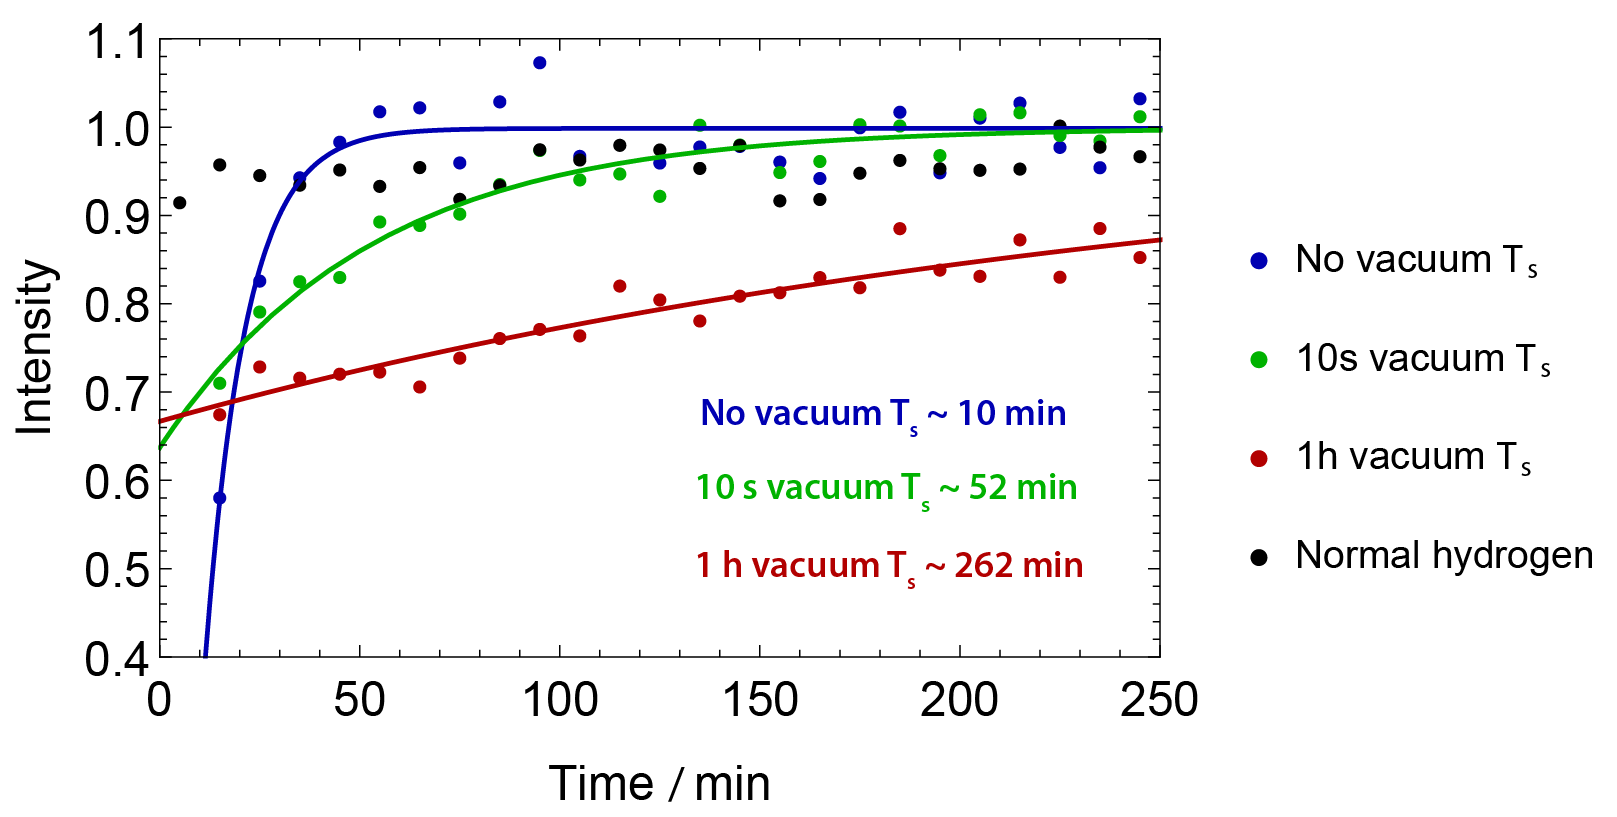
\includegraphics[width=\columnwidth]{PDMS-Ts.png}
  \caption{Ortho-para conversion of hydrogen in PDMS after various times
  under vacuum.}
  \label{fig:ph2conv}
\end{figure}

The detectable thermal signal in the ortho-para conversion experiment is
given by
$(1 - \frac{1}{3}\left( 4f - 1 \right))$,
where $f$ is the
para-enrichment level of the H\textsubscript{2} gas.
Therefore, the equilibrium ratio of
$f = 0.25$ gives a signal of 1, and pure parahydrogen gas gives no
signal. Hence, our signal starting at 50\% enrichment should vary from
2/3 to 1.
The data was fit to a function of the form
$(A - B\ e^{- \frac{t}{T_{s}}})$, with $A$, $B$ and $T_{s}$ as
variables.
The $T_s$ under no vacuum of \~10 min lead to the assumption that no significant
relaxation would occur during the transport of H$_2$ through the PDMS membrane.

\subsection{Reaction Scheme}

\begin{figure*}[ht]
  \centering
  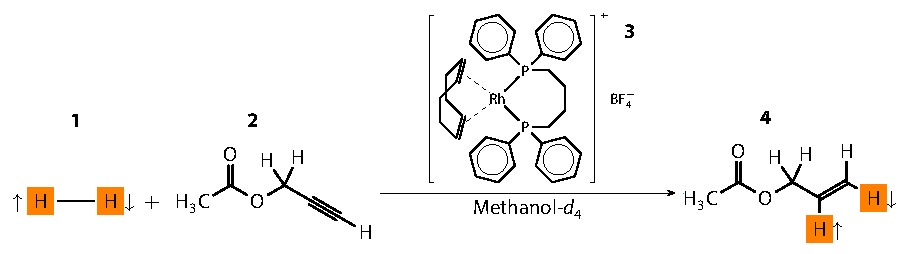
\includegraphics[width=15cm]{mu1y11-ph2c-fi-190511-paa-reaction-scheme.pdf}
  \caption{
    Scheme of the reaction used in the PHIP@chip experiment. Hydrogen gas
    \textbf{1}
    enriched in parahydrogen reacts with propargyl acetate \textbf{2} in
    the presence of the Rh catalyst \textbf{3} to form allyl acetate \textbf{4}.
  }
  \label{fig:reaction-scheme}
\end{figure*}

The hydrogenation reaction system employed in the present work is shown in
\fig{fig:reaction-scheme}.
Para\-hydrogen-en\-riched hydrogen gas $\mathbf{1}$ was
allowed to react with propargyl acetate $\mathbf{2}$, in the presence of
a rhodium catalyst $\mathbf{3}$. The substrate $\mathbf{2}$ was chosen in
view of future studies based on side-arm hydrogenation (SAH)
\cite{Reineri:2015he,cavallari201813,cavallari2015effects}. In SAH, the
polarisation of the $^1$H nucleus is transferred to a neighbouring $^13$C
and the moiety that has been hydrogenated is removed. SAH techniques can
help to bring generality to the PHIP technique as they eliminate the need for
the hyperpolarized target molecule to contact unsaturated bonds.

\subsection{ALTADENA}

In order to verify that the parahydrogen transfer on chip was possible, an
experiment was performed whereby the parahydrogen transfer was microfluidic
and ‘on chip’ but the detection was performed in a conventional NMR tube and probe.

This ALTADENA type experiment involved the addition of para enriched hydrogen
gas to propargyl acetate outside the magnetic field in a device shown in \fig{fig:AltadenaChip}. This device
is a simpler version of the one eventually used.
It features 3D printed holders that are used to deliver the gas and liquid as
well as seal against any liquid or gas leak. The chip is made from a single 500
$\mu$m thick layer of PMMA with serpentine paths for liquid and gas flow. B in the
\fig{fig:AltadenaChip} shows the path structure in the chip as well as the hydrogen and fluid paths
respectively.

\begin{figure}[ht]
  \begin{center}
  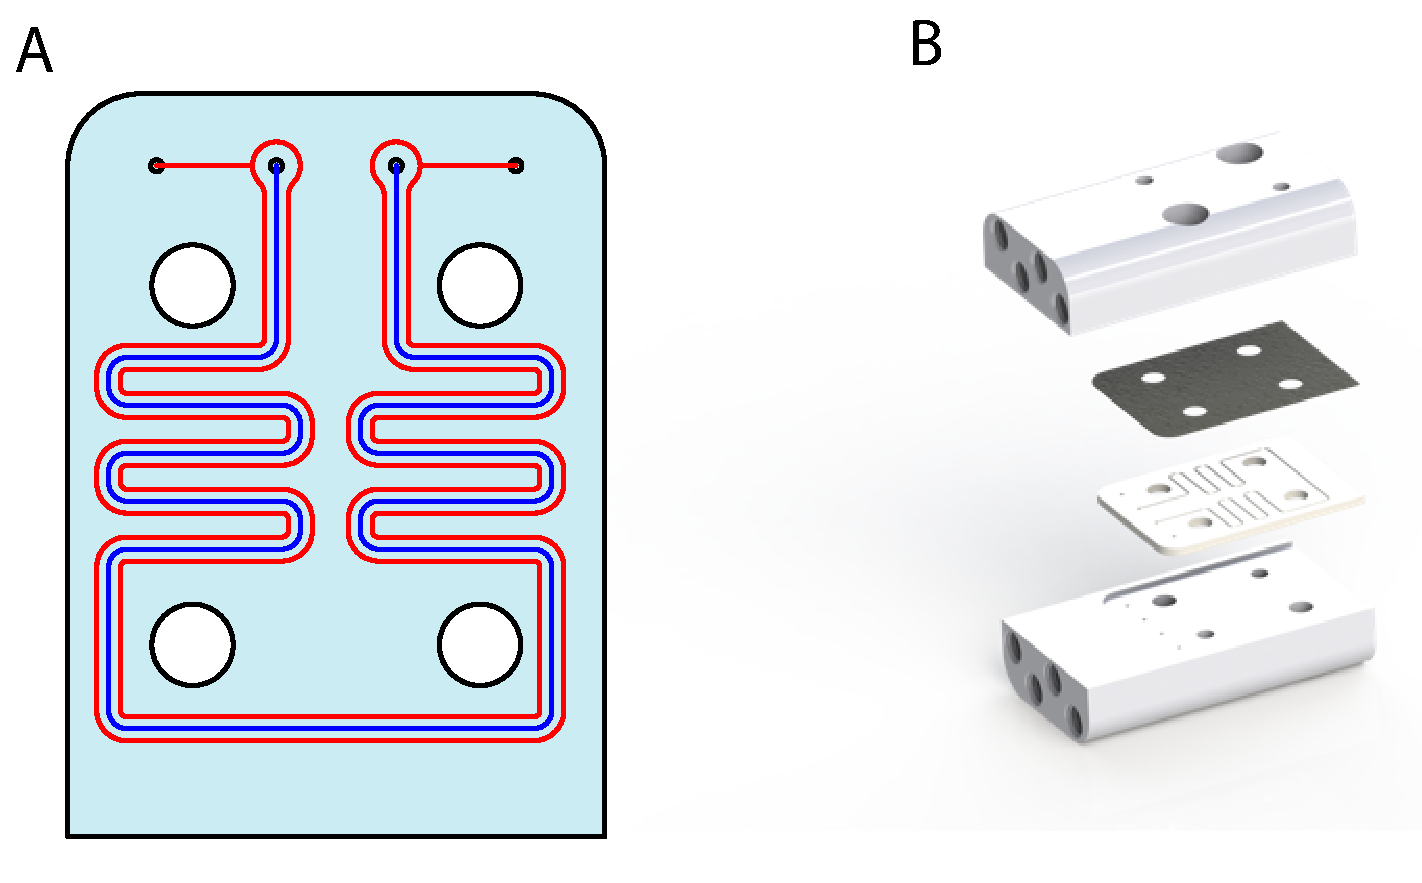
\includegraphics[width=\columnwidth]{ALTADENA-FIG.pdf}
  \end{center}
  \caption{A) Liquid channel (blue) and hydrogen channel (red) as scored
  onto the PMMA layer of the device. B) A 3D render of the hydrogenation device
  used for the ALTADENA experiements.}
  \label{fig:AltadenaChip}
\end{figure}

The set-up for this experiment employs a syringe pump, the hydrogenation device
outside the magnet and a standard 5 mm NMR tube inside the 16.5 T magnet. The device
was pressurised with 5 bar of 50\% enriched parahydrogen and allowed to equilibrate
for some time. Then, 100 $\mu$l was flown through the device at a flow rate of 1000
$\mu$l min$^{-1}$ this was done to ensure the sample from the experiment would reside
completely in the sensitive area. For the ALTADENA, 350 $\mu$l was flown through
the device and collected in the magnet. A $\pi$/2 pulse was applied and the spectra
recorded the result of the experiment is shown in \fig{fig:AltadenaResults}.

A comparison is shown between scans taken of the same experiment, in \fig{fig:AltadenaResults} i) spectra
from an experiment with thermal hydrogen and ii) one with parahydrogen. The parahydrogen
ALTADENA signal (ii) exhibits the characteristic inverted peaks and a much higher signal
to noise ratio (SNR) and gives enhancement by comparison of the SNR of around 200.
This result provided a proof of principle that parahydrogenation induced polarization (PHIP) on a chip
was possible by bubble free transfer through a PDMS membrane in our devices.

\begin{figure}[ht]
  \begin{center}
  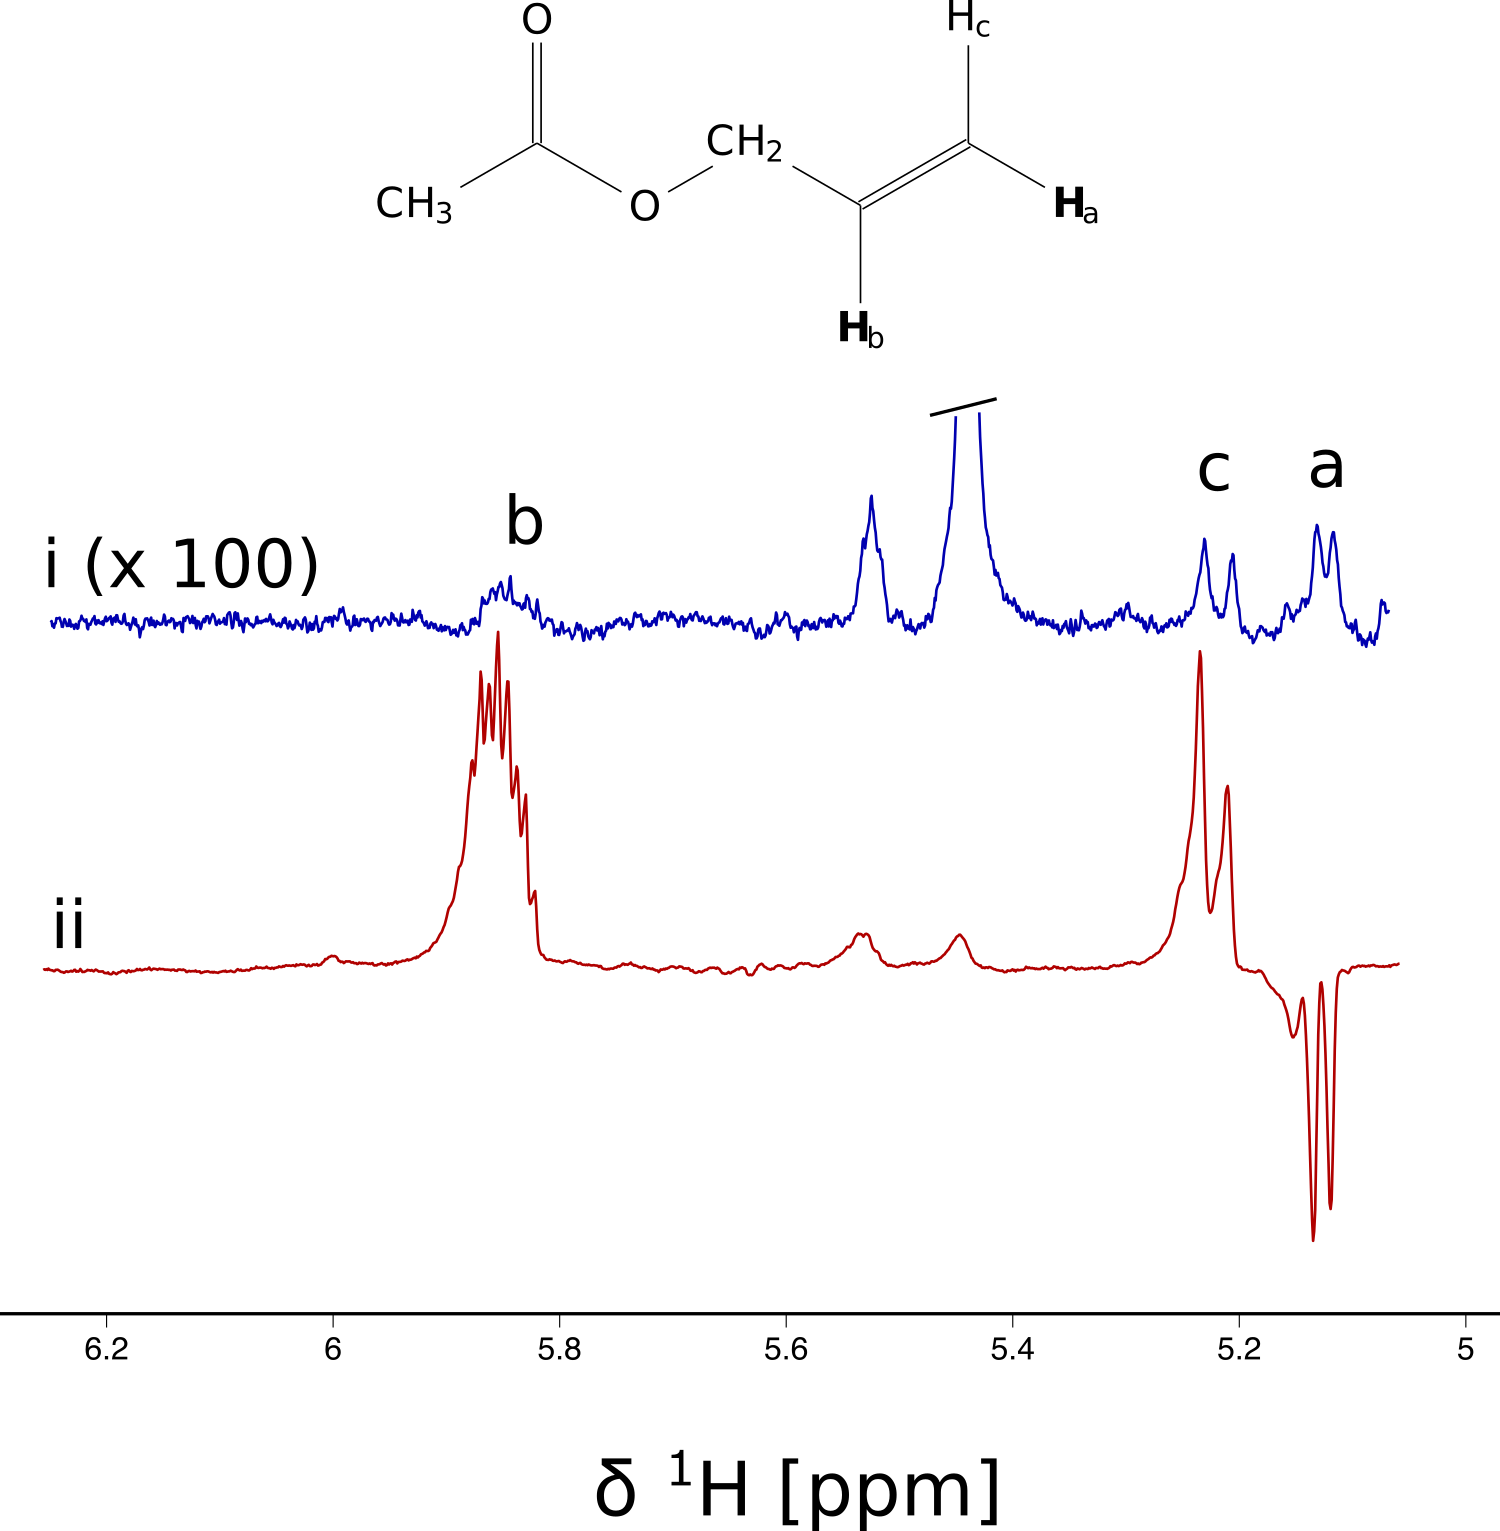
\includegraphics[width=7cm,keepaspectratio]{Altadena-Signal-comp.png}
  \end{center}
  \caption{Spectra obtained from i) a thermal hydrogenation and ii) a parahydrogenation
  of propargyl acetate to give allyl acetate with hydrogens derived from parahydrogen labelled a and
  b. By comparison of SNR the enhancement for the ALTADENA experiment is ~200. }
  \label{fig:AltadenaResults}
\end{figure}

\newpage

\subsection{PASADENA}

\begin{figure}[!ht]
	\centering
	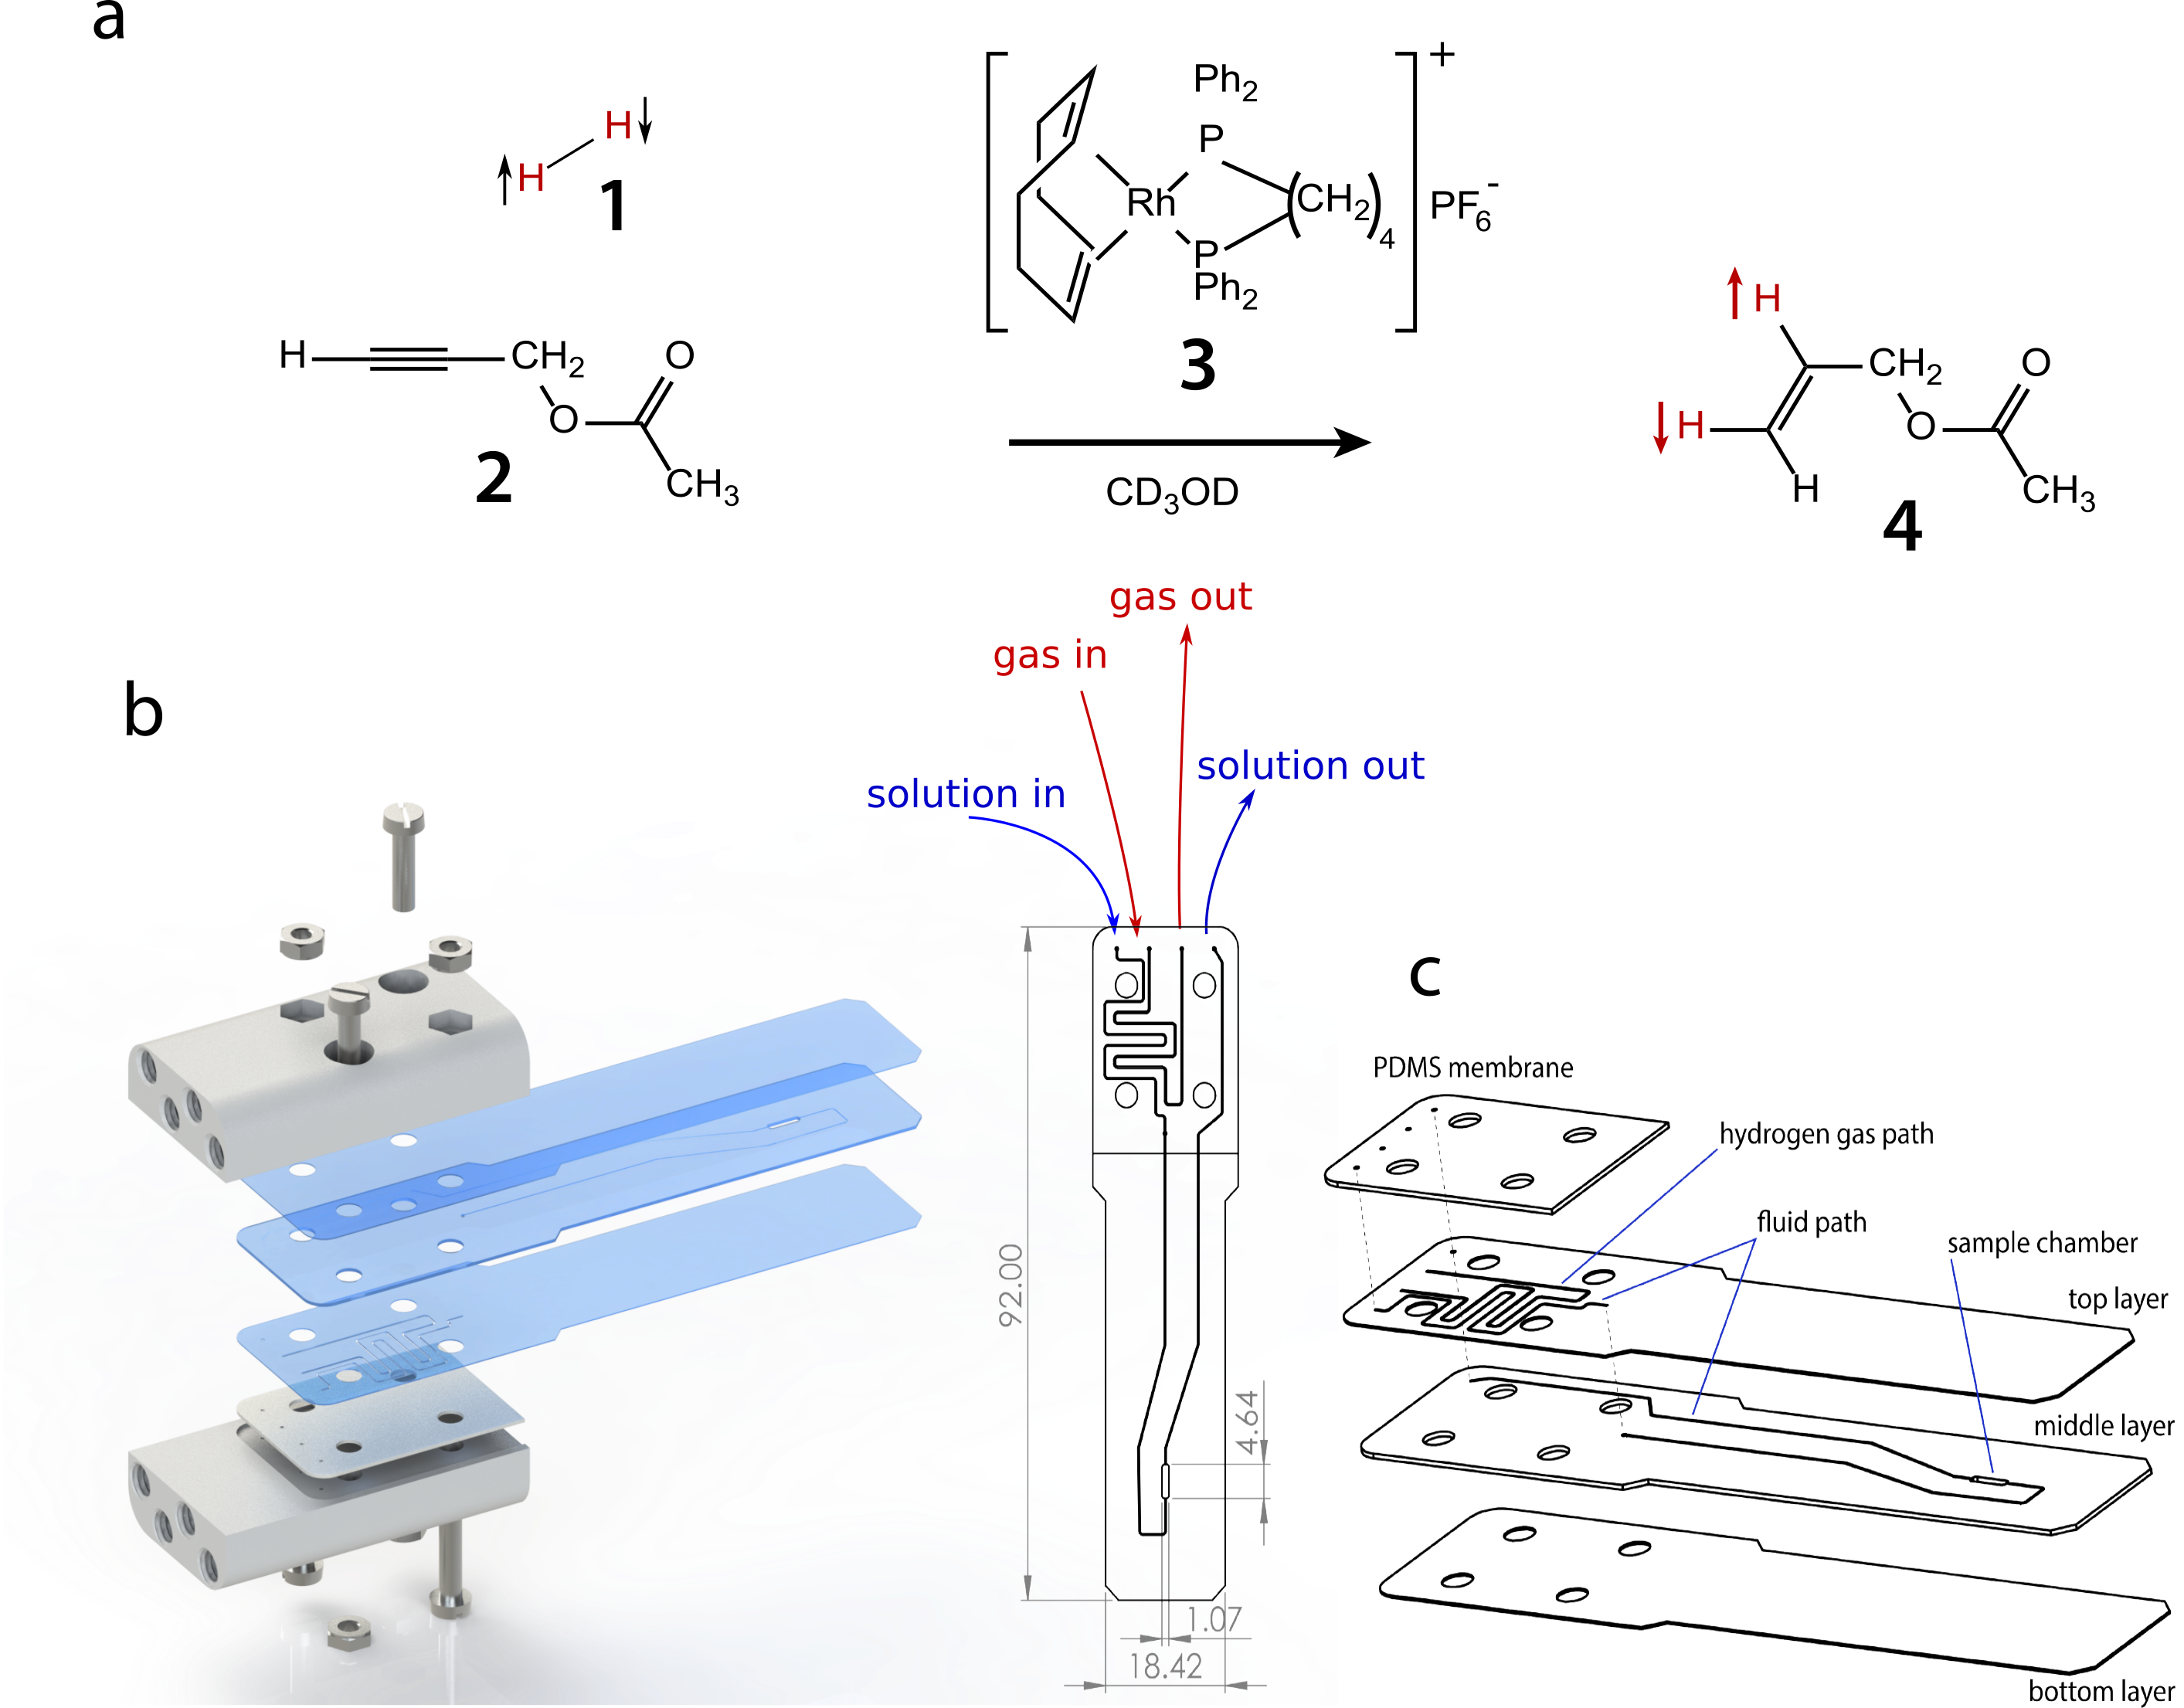
\includegraphics[width=10cm]{mu1y11-ph2c-fi-190117-fig1.png}
	\caption{Overview of the PHIP@chip device.
		% a: scheme of the hydrogenation reaction;
    %
    a: outline drawing of the chip (dimensions in mm).
		b: CAD rendering of the chip assembly with individual chip layers
		separated, consisting of the PMMA chip, PDMS membrane, and two 3D
		printed holders with threads for the gas and fluid connections.
    The hydrogen gas
		diffuses through the PDMS membrane into the flowing liquid.
		}
	\label{fig:phip@chip1}
\end{figure}

\begin{figure}
  \begin{center}
  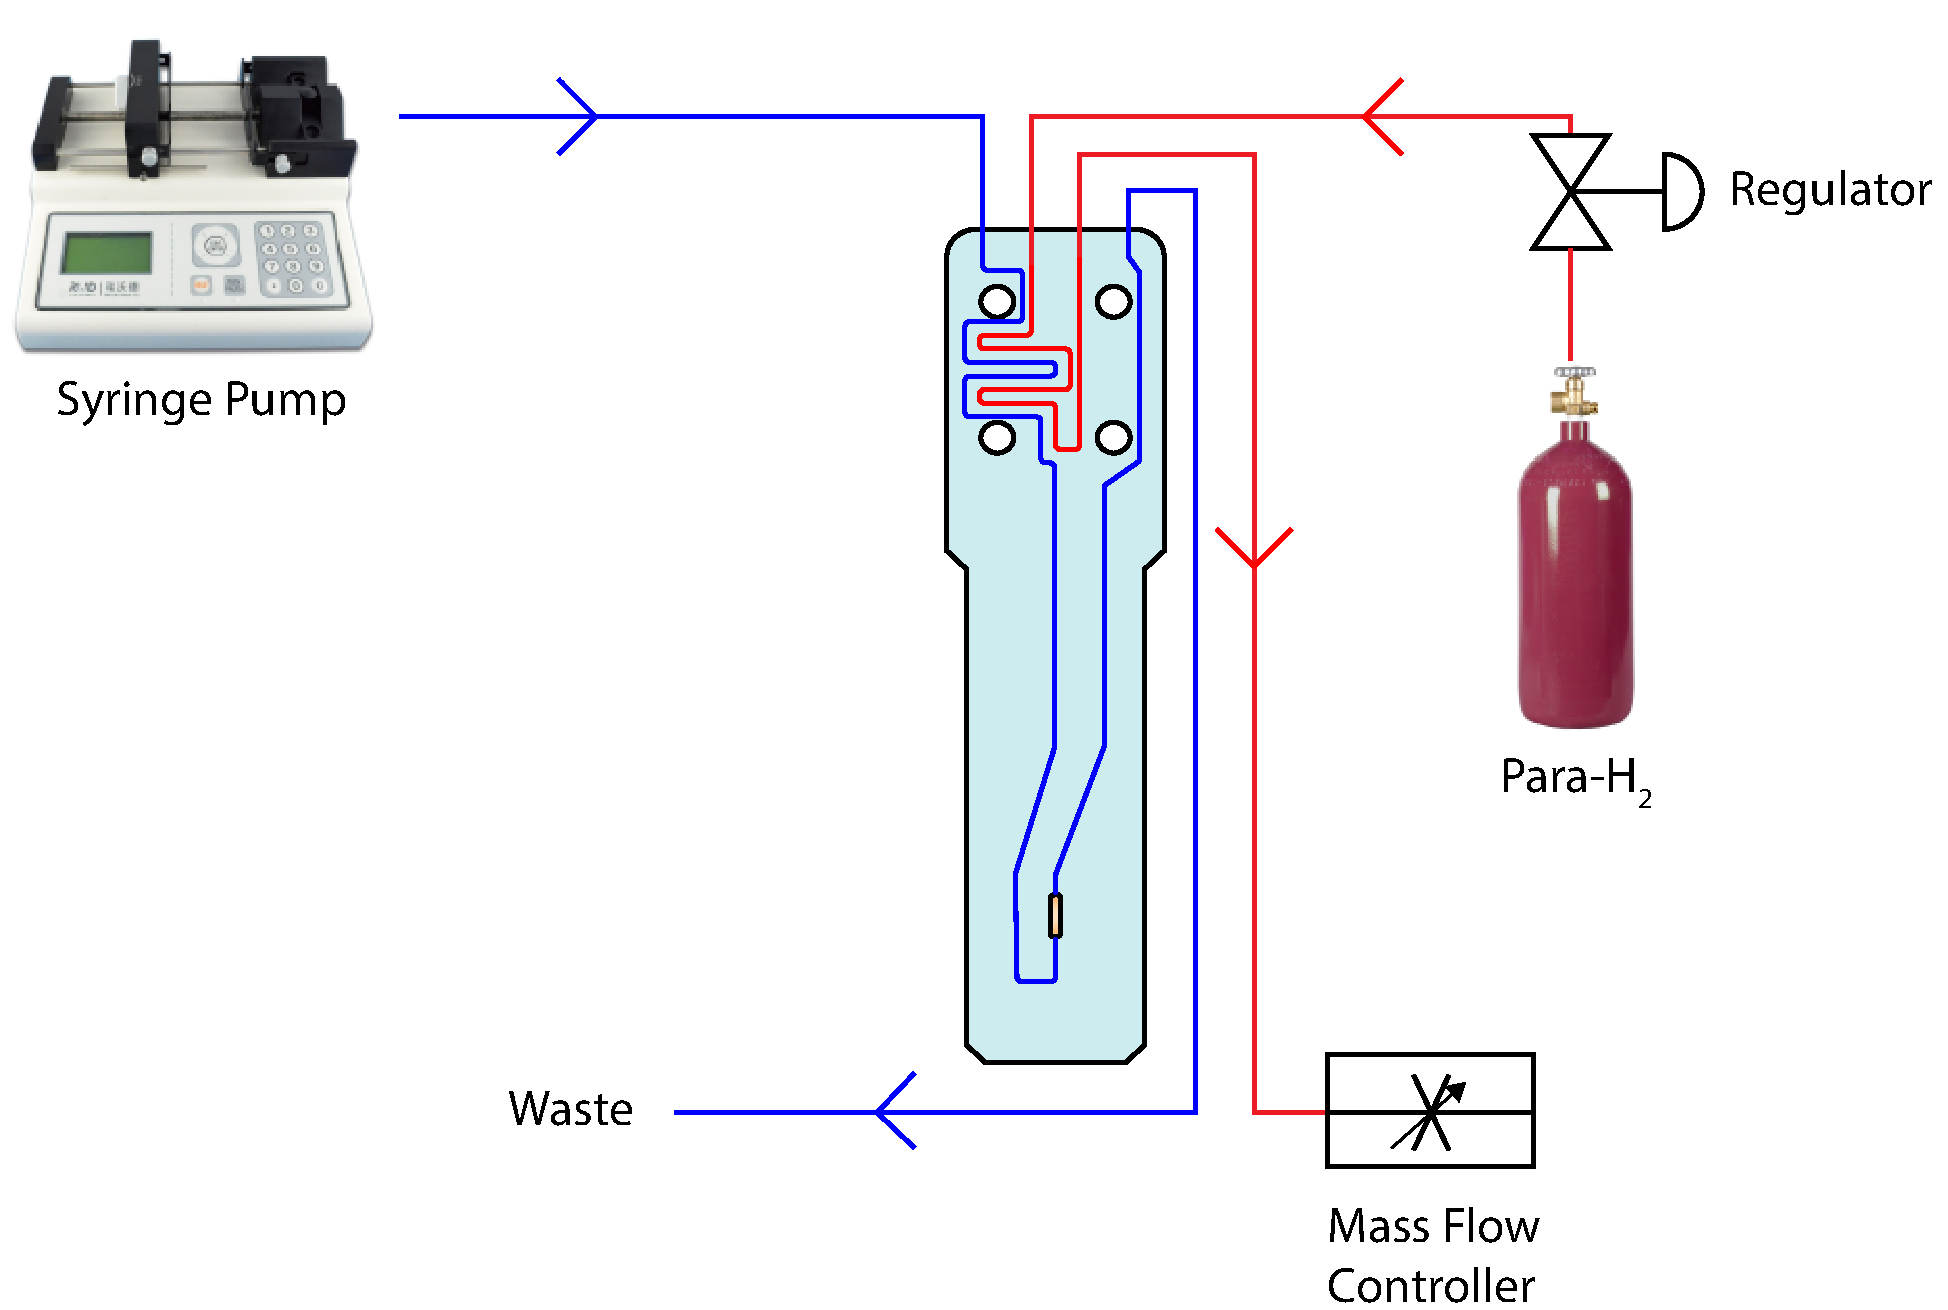
\includegraphics[width=\columnwidth]{PHIP-setup.pdf}
  \end{center}
  \caption{Drawing of PHIP@chip setup. It shows the solution (blue line)
  of propargyl acetate, catalyst and methanol being fed into the magnet
  via a syringe pump. Simultaneously, parahydrogen (red line) is fed in
  at the desired pressure and regulated by a mass flow controller to a
  flow rate of 20 ml$\text{min}^{-1}$. Both of these are fed into the
  microfluidic device depicted in \fig{fig:phip@chip1}}
  \label{fig:SetUp}
\end{figure}

\fig{fig:phip@chip1} shows the microfluidic device used for the
present study. It consists of a chip made from PMMA, which houses a sample
chamber of 2.5~$\mathrm{\mu L}$ volume that aligns with the transmission line
detector of a home-built NMR probe assembly, which was fitted inside of an
11.7~T NMR magnet.
Fluid is flowed through the chip by means of a syringe pump
installed outside of the magnet bore; connections are made through threaded
ports in the two 3D-printed holders shown in \fig{fig:phip@chip1}b.
Para-enriched H\textsubscript{2} gas at 5~bar above ambient pressure flows
through a second
channel in the chip, which runs in
the immediate vicinity of the liquid channel. A depiction of the set-up is given in \fig{fig:SetUp}.


\begin{figure}
	\centering
	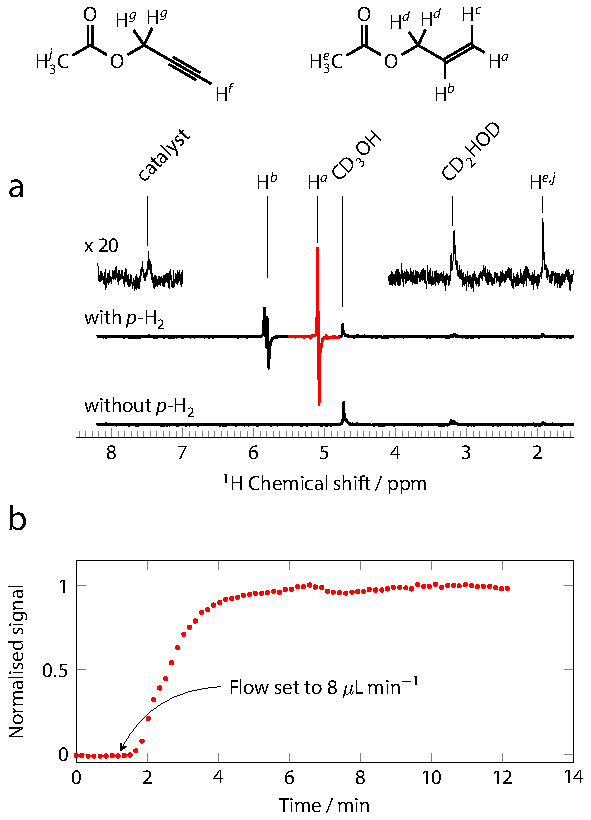
\includegraphics[width=8cm]{mu1y11-ph2c-fi-100506-buildup-curve.pdf}
	%
	\caption{a: Single-scan proton NMR spectrum obtained with
  parahydrogen at 5 bar using the PHIP@chip setup at a continuous
  flow rate of 8~$\mu$L$\,\text{min}^{-1}$ (top trace with enlargement).
  Antiphase doublets from the two
	hyperpolarized protons $\mathrm{H}^a$  and $\mathrm{H}^{b}$ are
  clearly visible at 5.2~ppm and 5.9~ppm, respectively. Without
  parahydrogen, these signals are not observed (bottom trace).
	%%
	b: Buildup of the hyperpolarized signal ($\mathrm{H}^{a}$)
  after initiation of flow.
	%
	}
	\label{fig:phip@chip2}
\end{figure}


The chip consists of three laser-cut layers of poly methylmethacrylate (PMMA)
bonded together, as shown in \fig{fig:phip@chip1}b. Channels in the
left part of the chip, where it is clamped between the holders, are cut through
the top layer, while they are scored into the middle layer of the chip (and
hence sealed from the outside) in the free part of the device.
Within the clamps, the exposed channels are sealed by means of a PDMS membrane.
The flowing liquid as well as
the pressurised hydrogen gas are therefore exposed to the PDMS layer,
which serves as a diffusion bridge for the hydrogen.
The holders, made by 3D printing, keeps the membrane and the chip aligned,
and maintains mechanical pressure to ensure sealing. Channels
inside the holders guide the fluid and gas to and from
the four access points at the top end
of the chip, as shown in \fig{fig:phip@chip1}b.
The PDMS membrane acts both as a diffusion conduit for hydrogen gas
and as a fluid seal.
In a crucial difference to the otherwise similar geometry of the
hydrogenation chip used by Bordonali et al\cite{Bordonali:2019jq},
the gas and liquid channels are arranged side by side, and molecular
hydrogen diffuses through the bulk of the PDMS membrane rather than across the
membrane. Clamping the PDMS membrane onto the chip using the
holders, makes it possible to use large gas pressures (up to 5 bar in
the present experiments). This would be difficult to achieve in the
chip presented by Bordonali et al, which has the liquid and gas channels
arranged on opposite sides of the membrane.

\newpage

\subsection{Signal Analysis}

\fig{fig:phip@chip2}a shows a single-scan proton NMR spectrum
obtained from a steady-state PHIP@chip experiment (top trace), compared
to the spectrum obtained without parahydrogen (bottom trace).
The hyperpolarized spectrum is dominated by an antiphase doublet,
centred at 5.17~ppm, and an antiphase multiplet at 5.92~ppm, corresponding to
protons in the $\mathrm{H}^a$ and $\mathrm{H}^b$ positions of the
hydrogenation product \textbf{4}.
The PDMS membrane is equilibrated with para-enriched hydrogen gas, which is
supplied from an aluminium storage tank at a regulated pressure of 5~bar. The
gas flow rate is kept constant at 20~$\text{mL}\,\text{min}^{-1}$ by means of a
mass flow controller placed after the chip. This ensures that the gas channel
always contains fresh para-enriched hydrogen gas at the design pressure of
5~bar. The fluid channel of the chip is pre-filled with a solution of 20~mM
precursor $\mathbf{2}$ and 5~mM catalyst $\mathbf{3}$ in methanol-$d_4$. NMR
spectra are acquired every 30~s, using a $\pi/4$ excitation pulse.  The fluid
channel is connected to a syringe pump situated outside the NMR magnet.
The
liquid flow is started by setting the target flow rate on the syringe pump to
8~$\mathrm{\mu L\,\text{min}^{-1}}$ (marked by an arrow \fig{fig:phip@chip2}b).
The NMR signal intensity begins to rise about 30~s later, and reaches a steady
state after about two minutes.

Using normal hydrogen gas, a fully labelled spectrum of the reaction mixture
was obtained using a lower flow rates whilst maintaining
the 5 bar of hydrogen pressure. This allowed the solution to saturate with
methanol and facilitated the quantification of the product and dissolved hydrogen.
A fully labelled spectrum obtained using a flow rate of 2$\mu$L$\text{min}^{-1}$
is shown in \fig{fig:LabelledSpec}

\begin{figure}
  \begin{center}
  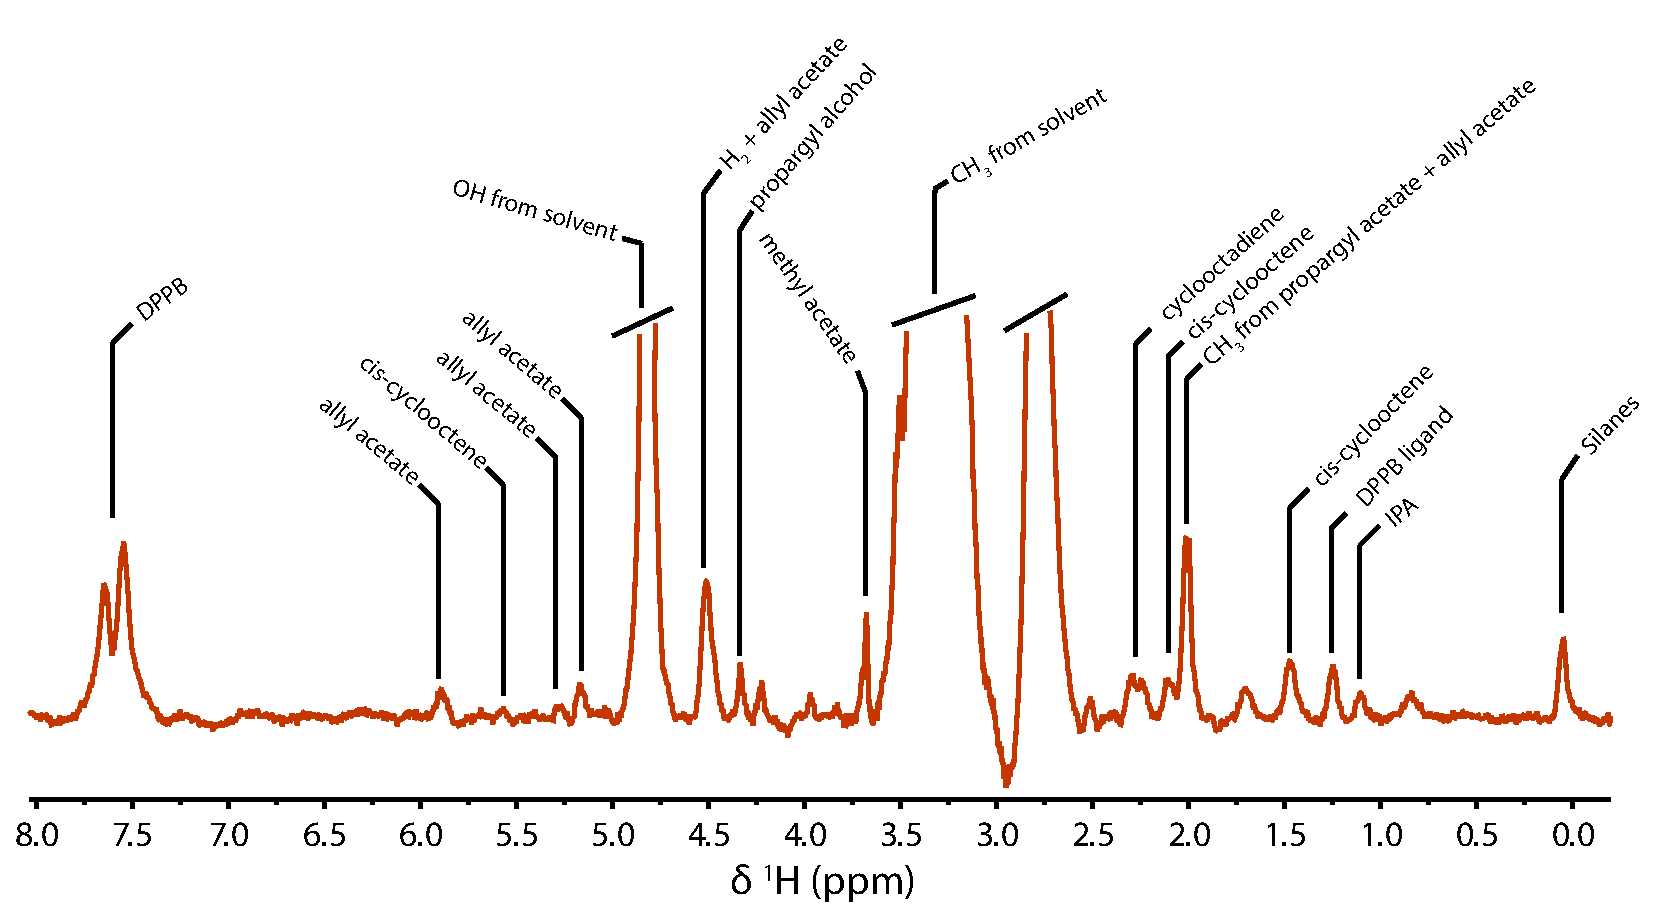
\includegraphics[width=\columnwidth]{Labelled-spectrum.pdf}
  \end{center}
  \caption{Labelled $^1$H spectrum acquired using a flow rate of 2$\mu~l \text{min}^{-1}$
  and a normal hydrogen pressure of 5 bar. The spectrum was collected using 64 transients
  with a delay of 5 seconds.}
  \label{fig:LabelledSpec}
\end{figure}

\newpage

\subsection{Hydrogen Transport}

\begin{figure}
  \begin{center}
	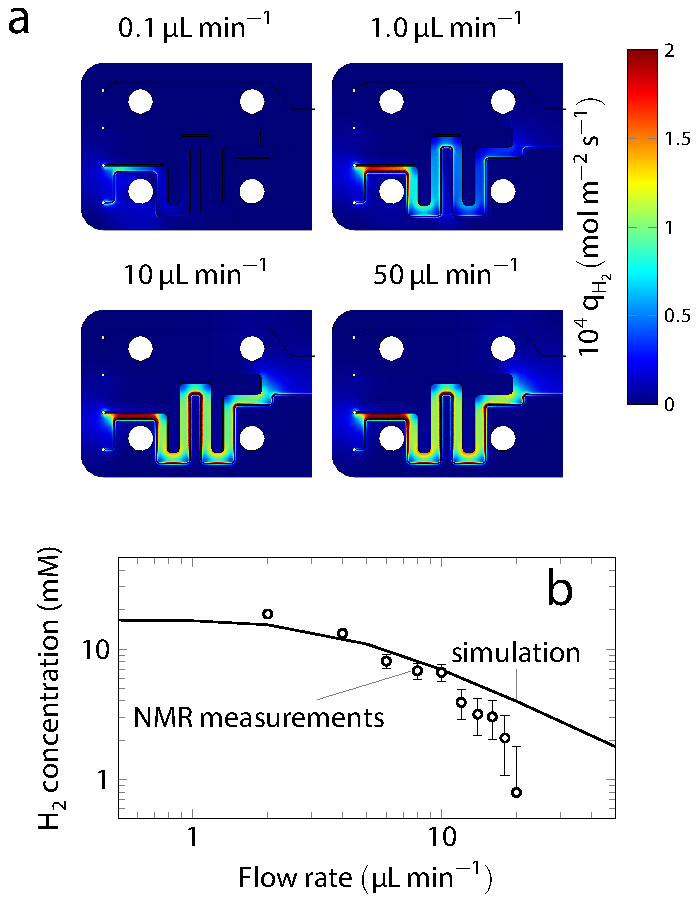
\includegraphics[width=7cm]{mu1y11-ph2c-fi-190117-h2fluxsim.pdf}
  \end{center}
	\caption{
		Finite element simulation of hydrogen uptake. a: Diffusive hydrogen
		flux in the PDMS membrane for different liquid flow rates;
    %
		b: final hydrogen concentration in flowing methanol as a function of
		flow rate. Solid line: simulation, open circles: NMR measurements.
	}
	\label{fig:h2fluxsim}
\end{figure}

The hydrogen transport through the membrane and its uptake into the flowing
liquid was simulated using two coupled finite element models: a dilute species
diffusion model for hydrogen gas in the PDMS membrane, and a dilute species
diffusion and convection model for hydrogen dissolved in the flowing liquid. The
hydrogen partial pressures at the liquid/PMDS interface are constrained to be
equal, and the hydrogen partial pressure at the gas/PDMS interface was set to a
fixed value of 5~bar. \fig{fig:h2fluxsim}a shows the diffusive flux of hydrogen
through the PDMS membrane.  Since the gas/PDMS interface acts as a source, and
the liquid/PDMS interface as a sink for hydrogen, the flux is strongest where
the two channels are in close proximity. At the lowest flow rate, significant
transport only takes place in a very small area, and the liquid is saturated
with hydrogen within the first few mm of the path which is in contact with the
PDMS. The higher the flow rate, the further the area of significant flux extends
downstream. At about 10~$\mathrm{\mu l \,min^{-1}}$, the hydrogen flux covers
the entire length of the area between the liquid and gas channel interfaces. The
finite element model also predicts the resulting concentration of hydrogen in
the liquid (methanol) as a function of flow rate. This is shown by the solid
line in  \fig{fig:h2fluxsim}b. The circles represent NMR measurements. At
flow rates between 2 and 10~$\mathrm{\mu l min^{-1}}$, experimental results are
in good agreement with the simulation. At higher flow rates, however, the
experimentally observed hydrogen concentrations are significantly lower than the
predictions. It is currently unclear what causes this discrepancy; possibly high
flow rates lead to deformation of the PDMS layer over the liquid channel and
thus change the uptake geometry. At flow rates below 10$\,\mathrm{\mu l
\,min^{-1}}$, the simulation and experiments both indicate that the flowing
solvent is nearly saturated with hydrogen.


\subsection{Sensitivity and Limit of Detection}

\begin{figure}
	\centering
	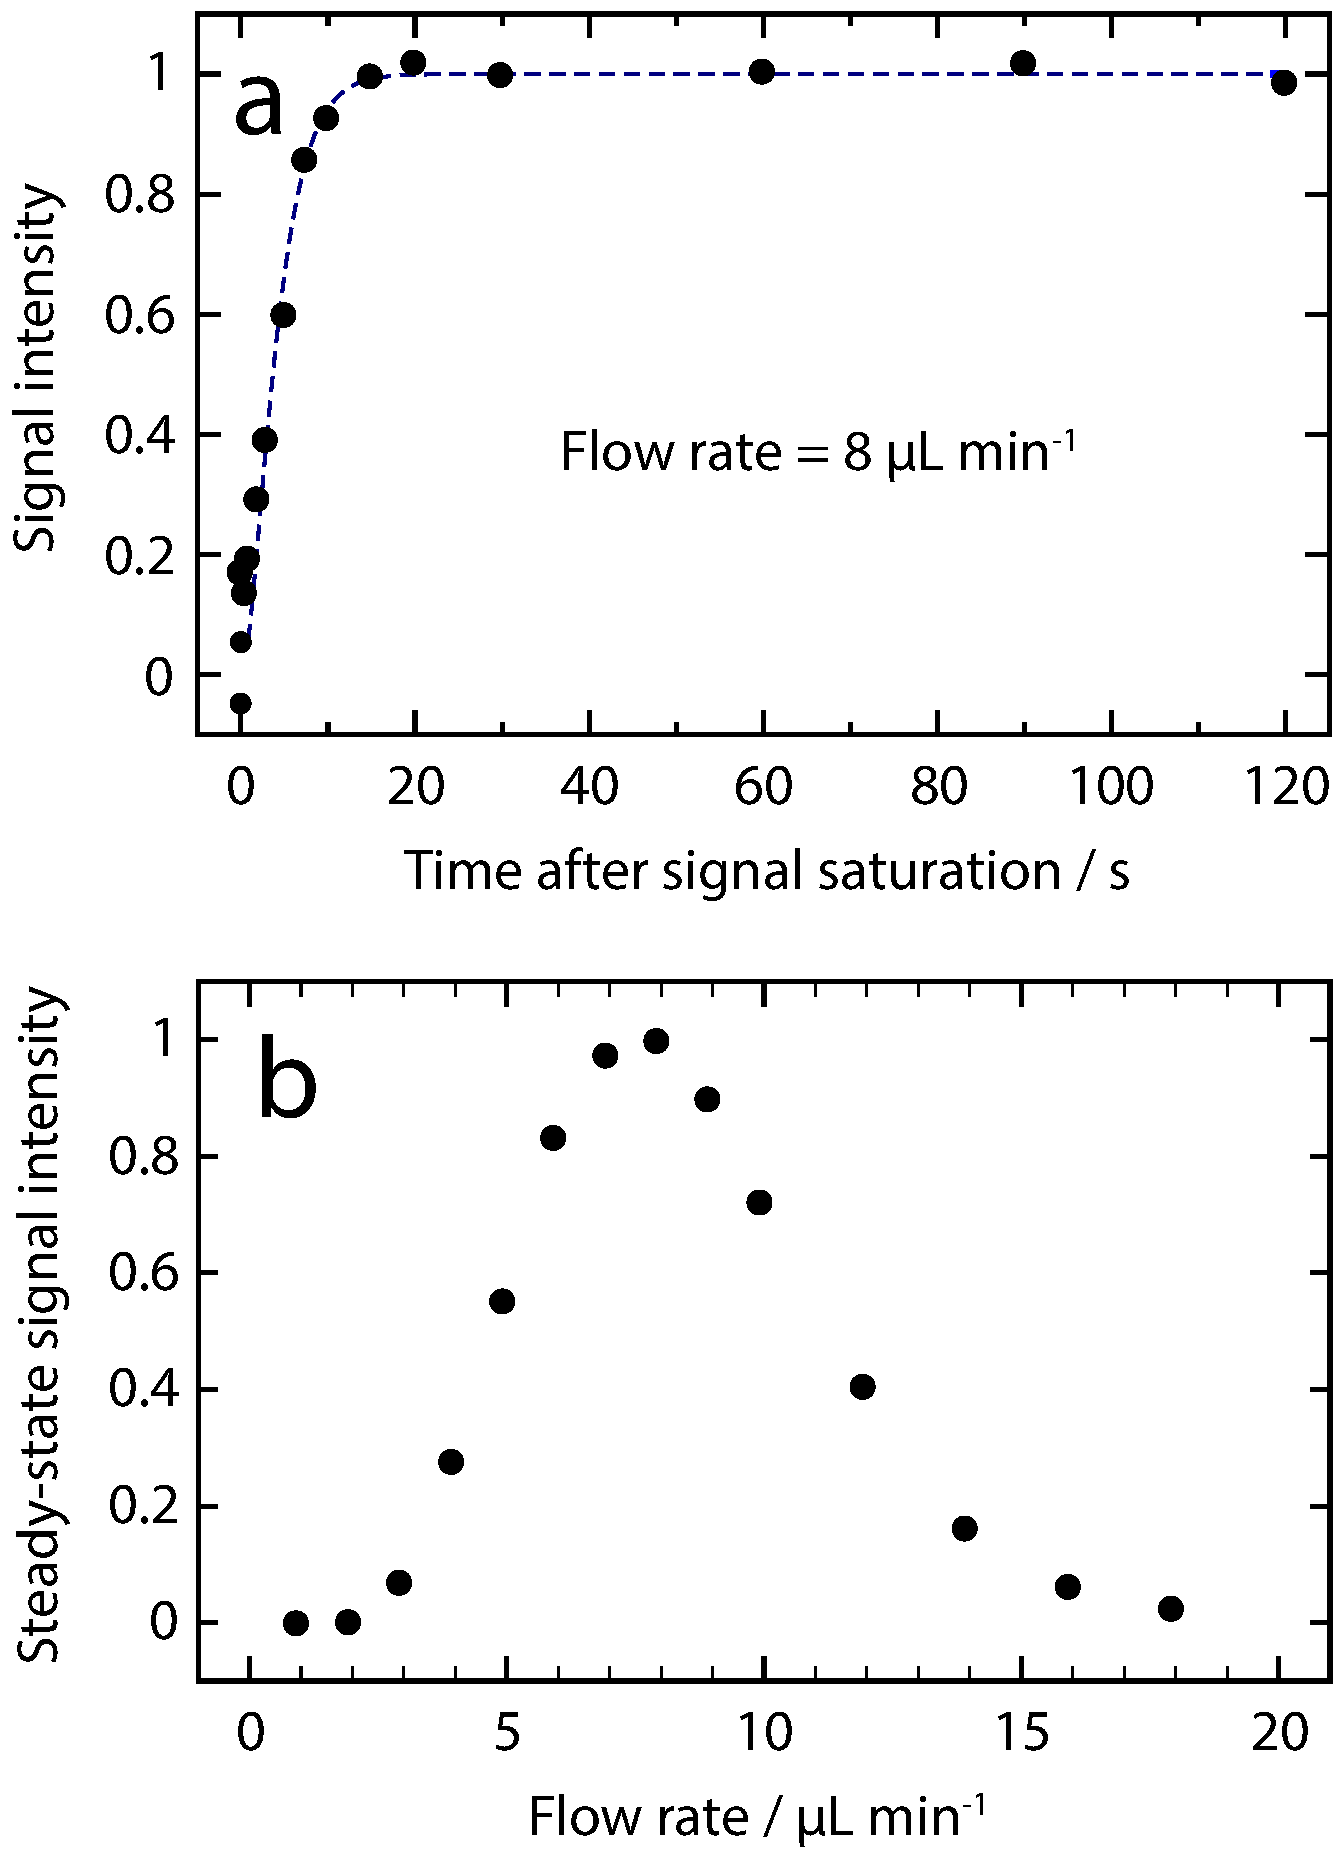
\includegraphics[width=7cm]{mu1y11-ph2c-190510-satrec-summary.pdf}
	\caption{Saturation recovery results.
  a: Signal buildup at constant
	flow rate after saturation (solid dots: measured data points,
  the dashed line is a guide to the eye);
	b: Magnitude of the steady-state signal after full recovery (at least
	100~s after saturation) as a function of flow rate. A clear maximum
	at 8~$\mu\mathrm{L}\,\text{min}^{-1}$ is observed.}
	\label{fig:satrec-summary}
\end{figure}


Clearly, the steady-state signals observed at constant flow rate are the result
of a dynamic equilibrium between the rate of hydrogenation, the rate of
transport of the hydrogenated product to the sample chamber and its removal
from it, and spin-lattice relaxation. In order to probe the interplay of these
factors, the NMR signal was suppressed by saturating the spin populations
with a train of 512 $\pi/2$ pulses separated by 100 $\mu$s delays.
The signal intensity was then measured as a function of the delay between the
end of the saturation train and the NMR excitation pulse.
\fig{fig:satrec-summary}a shows an example of the data thus obtained at a
flow rate $q=8\,\mathrm{\mu L\,\text{min}^{-1}}$.
The signal increases rapidly after saturation, reaching
steady-state levels after about 10~s.

\begin{figure}
  \begin{center}
  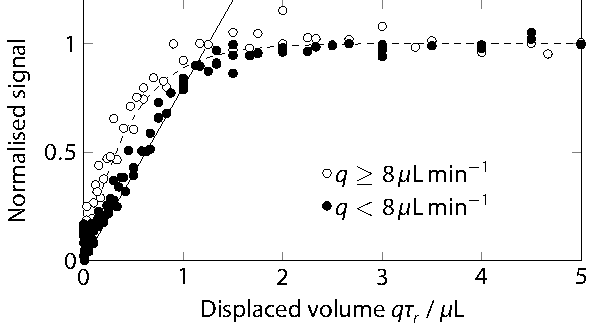
\includegraphics[width=0.45\textwidth]{mu1y11-ph2c-fi-190314-displaced-volume}
  \end{center}
  \caption{Signal recovery after saturation, normalised by the maximum signal
  observed at long recovery times. The horizontal axis is the volume
  moved through the chip during the recovery time $\tau_r$, i.e., $q\,\tau_r$,
  where $q$ is the flow rate. Filled circles correspond to flow rates below
  the optimum ($q<8\,\mu\mathrm{l}\,\text{min}^{-1}$), where as open circles
  are obtained at flow rates $q\ge 8\,\mu\mathrm{l}\,\text{min}^{-1}$. The solid
  and dashed lines are guides to the eye for the solid and open circle data points,
  respectively.}
  \label{fig:displaced-volume}
\end{figure}

The intensity of the steady-state NMR signal exhibits a clear maximum with flow
rate (\fig{fig:satrec-summary}b), reflecting a balance between hydrogen uptake,
reaction kinetics, and spin-lattice relaxation. The optimum, with the largest signal at
saturation, is reached at a flow rate of 8~$\mathrm{\mu L\,\text{min}^{-1}}$.
The nature of the stationary state established in the system at each
flow rate becomes clearer if the saturation recovery data is plotted in terms
of the volume displaced during the saturation recovery time $q\tau$, rather
than the recovery time itself, and normalised to the steady-state signal intensity
at each flow rate, as shown in \fig{fig:displaced-volume}. At flow rates below
the intensity maximum at $q<8\,\mathrm{\mu L\,\text{min}^{-1}}$ (solid
circles),
the data points collapse onto a curve that shows an initial linear increase
up to a displaced volume of about 1~$\mu$L, followed by rapid saturation to the
steady-state value. This behaviour clearly indicates that the
signal recovery in this regime is dominated by the convective fluid transport.
At these flow rates, a constant concentration of
hyperpolarized material is established in the flowing liquid upstream of the
sample chamber, and is simply carried back into view of the NMR detector
after the saturation pulses end.
The maximum signal is reached after a volume
of about 1.5~$\mu$L has been displaced. This is less than the capacity
of the sample chamber, reflecting the uneven velocity distribution inside it.
At flow rates above the optimum ($q\ge 8\,\mathrm{\mu L\,\text{min}^{-1}}$),
a somewhat different behaviour is observed. The initial recovery rate is
faster (\fig{fig:displaced-volume}, open circles), and appears to follow
an exponential rather than linear shape. This suggests that at these flow
rates, the stationary state is not yet established at the point where the
liquid enters the sample chamber, and therefore, the observed recovery
is dominated by the ongoing hydrogenation reaction.

\begin{figure}
  \begin{center}
    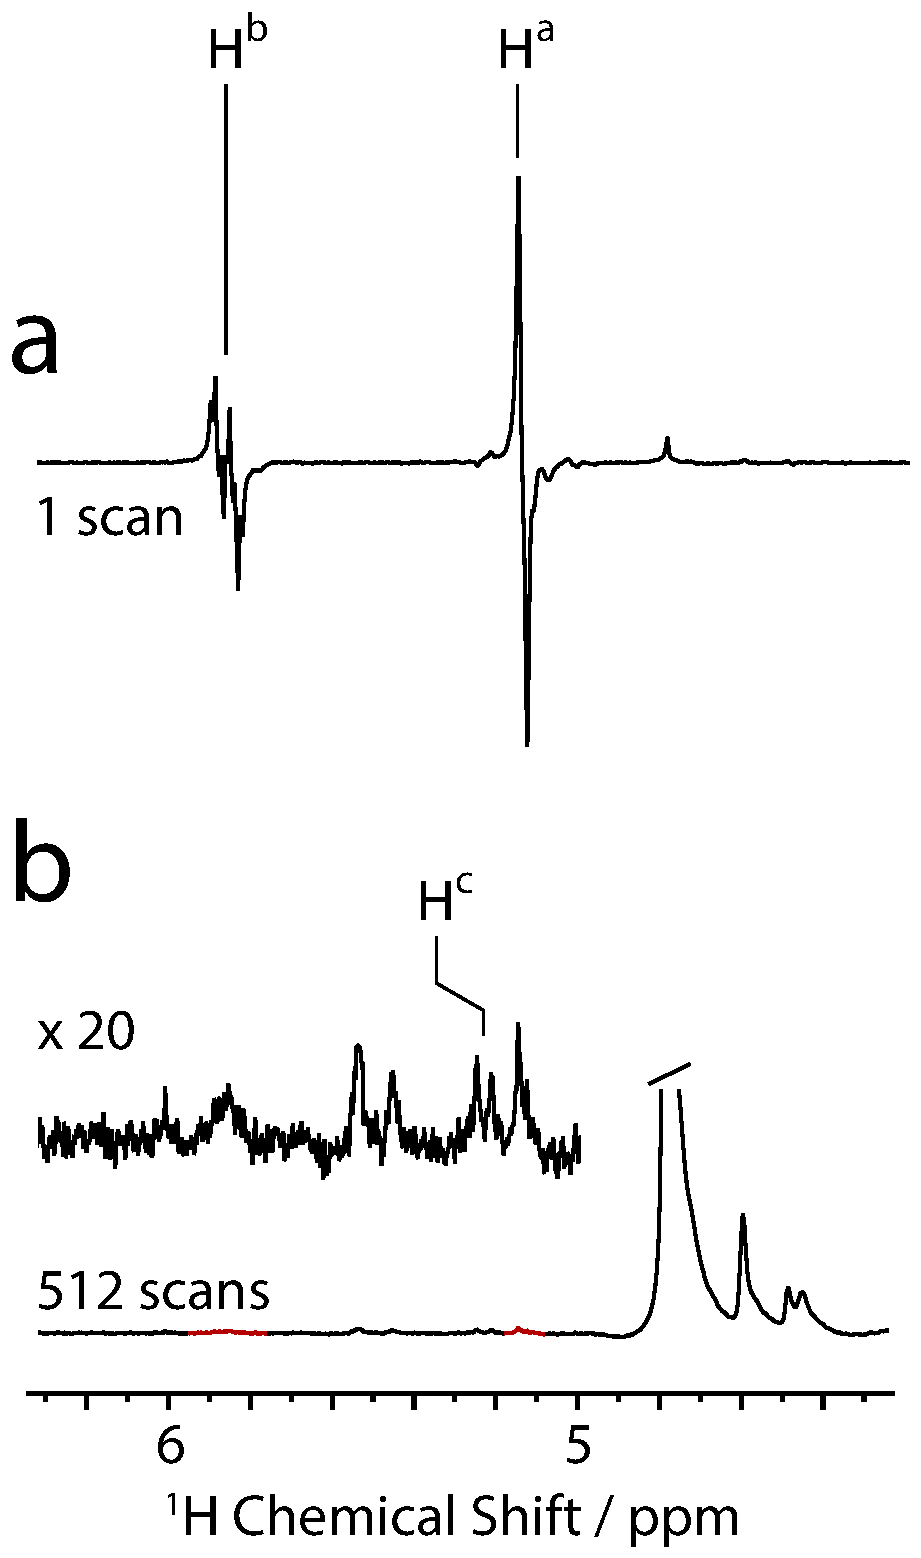
\includegraphics[width=6.0cm]{mu1y11-ph2c-fi-190510-pH2-vs-thermal512.pdf}
  \end{center}
  \caption{	a: Single-scan steady-state spectrum obtained at the optimum flow rate
  	with para-enriched H\textsubscript{2}; b: spectrum obtained at the same flow
    rate with hydrogen gas
  	in thermal equilibrium. 512 transients have been averaged. Signal enhancement by
  	PHIP was determined by comparing the integral of the positive lobe of
    the $\mathrm{H}^a$ signal in spectrum a to the
  	integral of the corresponding (purely absorptive) peak in spectrum b.}
  \label{fig:pH2-vs-thermal512}
\end{figure}

In order to determine the sensitivity of detection of the hydrogenation product
at the optimum flow rate, the experiment was repeated using normal hydrogen.
In this case, the signal from  protons $\mathrm{H}^a$ and $\mathrm{H}^b$
of the hydrogenation product \textbf{4}
are too weak to be observed above the noise in a single scan.
\fig{fig:pH2-vs-thermal512}
compares the hyperpolarized signal (a) to the averaged signal of 512 transients
obtained with hydrogen in thermal equilibrium (b).

Since the methyl group in the
precursor and the hydrogenation product contribute to the same signal at 2.05~ppm
(signal labelled $\mathrm{H}^{e,j}$ in \fig{fig:phip@chip2}a),
this signal can be used as a calibration standard, with a concentration of 20~mM
which is unaffected by the hydrogenation reaction. By comparing this integral to that
of the signal from the $\mathrm{H}^a$ protons, the concentration
of hydrogenated product can be
quantified. At a flow rate of 8~$\mathrm{\mu L\,\text{min}^{-1}}$, an allyl acetate
(product) concentration of $(0.29\pm 0.05)\,\mathrm{mM}$ was found, corresponding to a total
of $(0.725\pm0.125)\,\text{nmol}$ in the $2.5\,\mathrm{\mu L}$ sample volume.


This quantity can be used to determine the limit of detection of the
hyperpolarized product. The signal/noise ratio (SNR) in the spectrum shown in
\fig{fig:pH2-vs-thermal512}a is 400($\pm 10\%$), and the line width is $6\pm
0.5\,\text{Hz}$. The normalised limit of detection is given by \eqn{eqn:nLOD}\[
\text{nLOD}_\omega = \frac{3 n}{\text{SNR}\,\sqrt{\Delta f}}, \] where $n$ is
the amount of sample and $\Delta f$ is the signal bandwidth. In the present
case, one finds $\text{nLOD}_\omega = (2.2\pm
0.4)\,\text{pmol}\,\sqrt{\text{s}}$. Limits of detection in this range have so
far only been reported in very limited circumstances, including
chemically-induced dynamic nuclear polarization (CIDNP)
\cite{mompean2018pushing}, or or by making use of unconventional low-field
detection systems
such as force-detected magnetic resonance or optical detection methods\cite{Rugar:1992dm,Rugar:2004bc,Mamin:2007ff,Poggio:2010jf,
Maze:2008cs,Staudacher:2013kn,Rugar:2015by,McDermott:2002hp,
Budker:2007hz,Xu:2006kg,Blanchard:2013gs}. In the
present case, conventional inductive detection is used, and the full
resolution and specificity that make high-field NMR a useful
analytical tool are retained.

The mass limit of detection (LOD) for
protons at a magnetic field of 14.1~T (corresponding to a proton Larmor frequency
of 600~MHz) in state-of-the-art commercial NMR probes with a
conventional sample volume of 0.5~ml is approximately
100~$\text{nmol}\,\sqrt{\text{s}}$.
Microfluidic NMR systems can make use of miniaturised NMR detectors,
which benefit from a favourable scaling of the mass sensitivity
with detection volume \cite{Olson:1995vu,Badilita:2011td,Zalesskiy:2014hi}. At a size scale
of 2.5~$\mu\mathrm{l}$, a mass sensitivity around
$1\;\text{nmol}\,\sqrt{\text{s}}$
has been reported \cite{Finch:2016gv}.
However, due to the limited volume in such systems,
the \emph{concentration} sensitivity is very poor, such that
only compounds present at mM levels can be quantified
in microfluidic NMR systems. This situation gets worse as the detector
volume decreases. By contrast, many samples of interest, such as
metabolites in microfluidic culture systems, are only present
at $\mu$M levels.

In the present
case, the concentration limit of detection from \eqn{eqn:cLOD} is
\begin{equation}
\text{cLOD}_\omega =
\frac{\text{nLOD}_\omega}{V_s} = (0.88 ± 0.16)\mu\text{M}\sqrt{s}.
\end{equation}

From the ratio of the signal intensities in the thermal and hyperpolarized
spectra shown in \fig{fig:pH2-vs-thermal512}a and b, it is possible to estimate the
$\mathrm{^1H}$ polarization levels. In the thermal spectrum, the SNR is about
5:1, whereas it is 400:1 in the hyperpolarized spectrum. The thermal spectrum is
obtained from 512 transients, therefore the single transient thermal SNR would
be $5/\sqrt{512}\approx 0.22$. This leads to a signal enhancement factor of
$\epsilon\approx 400/0.22 \approx 1800$.

This can be compared to the expected signal enhancement given the enrichment
level of para-hydrogen used in the experiment. The ideal enhancement factor is
given by
\begin{equation}
	\epsilon_{id} =\frac{4x_p-1}{3\sqrt{2}} \frac{2 k_BT}{\hbar \gamma B_0},
\end{equation}
where $x_p$ is the mole fraction of parahydrogen in the feed gas, $\gamma$ is
the magnetogyric ratio, $B_0$ is the magnetic field, and $\hbar$ and $k_B$ are
Planck's and Boltzmann's constants, respectively.
The factor $\frac{1}{\sqrt{2}}$ reflects the use of a $\pi/4$ pulse for the
hyperpolarized experiment. At a temperature of $T=298$~K
and a magnetic field of $11.7$~T, and with $x_p=0.5$, this yields
$\epsilon_{id}\approx 5900$, which is a factor of 3.3 larger than the
experimentally observed enhancement factor. Therefore,
about 2/3 of the theoretically available spin order is lost to relaxation under
the present experimental conditions.

\subsection{2D NMR}

A great advantage of the continuously operating microfluidic PHIP system is the
ability to acquire many transients in succession under virtually unchanged
conditions.
This is difficult to achieve with bubbling hydrogen through a solution.
As a consequence, hyperpolarized multi-dimensional NMR spectra \cite{Mishkovsky:2008cl,Giraudeau:2009fn,Roth:2010hk,Lloyd:2012cf,Eshuis:2015ce,Kiryutin:2019hy}. have been recorded
either using automated reactors combined with NMR flow probes, \cite{Lloyd:2012cf,Eshuis:2015ce}
or using ultrafast acquisition techniques \cite{Mishkovsky:2008cl,Giraudeau:2009fn,Kiryutin:2019hy}.

The PHIP@chip setup allows straightforward acquisition of 2D spectra, using
conventional $t_1$ incrementation.
To demonstrate this, 2D TOCSY (Total Correlation
Spectroscopy) and HMQC (Heteronuclear Multiple Quantum Coherence) NMR spectra
of the reaction mixture at a flow rate of 8 $\mathrm{\mu L\,min^{-1}}$ have been performed.
The conventional
pulse sequences were modified by replacing the initial \(\pi\)/2 pulse with a
\(\pi/4\ \)pulse; these experiments are reffered to as ``PH-TOCSY'' (parahydrogen TOCSY) and
``PH-HMQC'' (parahydrogen HMQC).

\begin{figure}
	\centering
	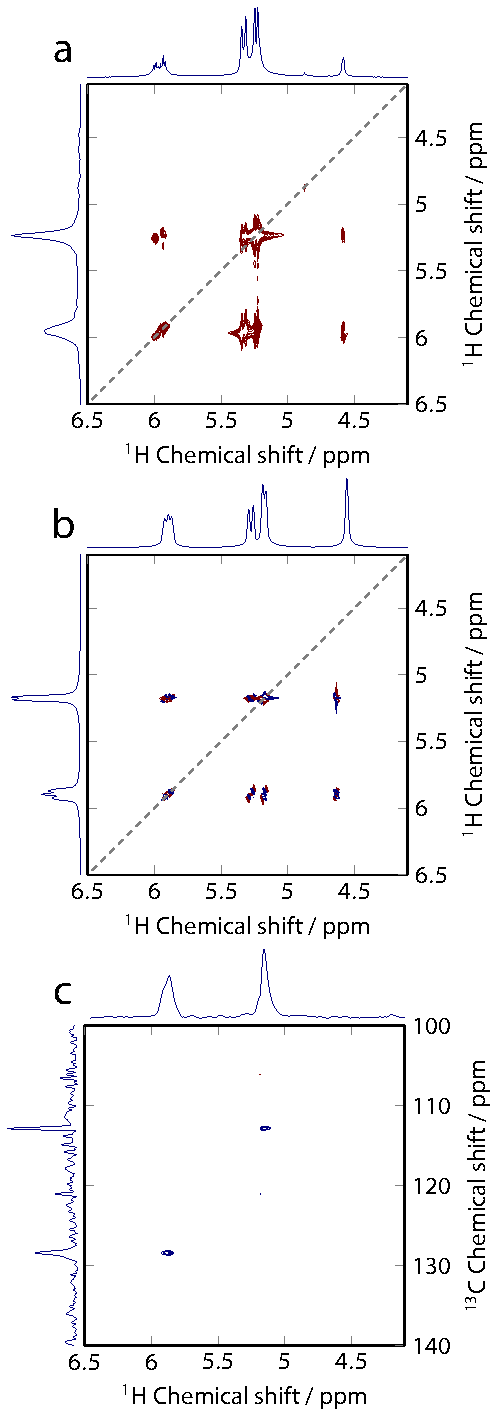
\includegraphics[height=20cm,keepaspectratio]{mu1y11-ph2c-fi-190505-PH-TOCSY-combined.pdf}
	\caption{
		The continuous flow PHIP@chip approach allows acquisition of
		two-dimensional spectra with very high sensitivity.
    %
    a: PH-TOCSY spectrum of the hyperpolarized reaction mixture,
		flowing at 8~$\mu\mathrm{L}\,\text{min}^{-1}$.
    %
    b: Simulated PH-TOCSY spectrum. The diagonal in the spectrum is marked by a dashed grey
		line. Only the protons originating from parahydrogen give signals on
		the diagonal; the polarization is transferred to the other locations by
		the isotropic mixing sequence. Both PH-TOCSY spectra are plotted in
    magnitude mode.
    %
    c: $^1$H-$^{13}$C PH-HMQC spectrum
		showing two separate multiplets, each correlating one of the two
		hyperpolarized protons with the directly bonded $^{13}$C spin.
}
	\label{fig:PH-TOCSY-HMQC}
\end{figure}

A PH-TOCSY spectrum acquired in 20 min is shown in \fig{fig:PH-TOCSY-HMQC}a.
A \emph{thermal equilibrium} TOCSY spectrum of this compound would be
expected to
contain diagonal peaks connecting the identical nuclear spins in the two
acquisition dimensions, and off-diagonal peaks connecting \emph{J}-coupled
spins. In the PH-TOCSY experiment, the diagonal peaks only appear
for the two parahydrogen proton signals, because they are the only spins
significantly polarised in the indirect dimension. The other protons
are only polarised during the isotropic spin-mixing step of the pulse sequence,
and hence do not appear in the indirect dimension. These protons only produce
off-diagonal peaks, connecting them to the parahydrogen pair.
As shown in \fig{fig:PH-TOCSY-HMQC}b, the simulated spectrum
closely corresponds to the experimentally observed one.

A \emph{thermal equilibrium} TOSCY spectrum of this compound would be expected to
contain diagonal peaks connecting the identical nuclear spins in the two
acquisition dimensions, and off-diagonal peaks connecting \emph{J}-coupled
spins. In this \emph{hyperpolarized} experiment, the diagonal peaks only appear
for the two parahydrogen proton signals, because they are the only spins
significantly polarised in the direct detection dimension. The other protons
are only polarised during the isotropic spin-mixing step of the pulse sequence,
and hence don't appear in the direct dimension. These protons only produce
off-diagonal peaks, connecting them to the parahydrogen pair.

A PH-HMQC spectrum acquired in 60 min is shown in \fig{fig:PH-TOCSY-HMQC}c.
It contains two peaks, linking the parahydrogen protons to the
\textsuperscript{13}C spins to which they have a direct
\textsuperscript{1}\emph{J}\textsubscript{CH} coupling.
An experiment of this kind, in which signals are
detected at full natural abundance of the \textsuperscript{13}C spins (about
1\%) in a 2.5~$\mu$L  detection volume, is only possible due to both the high
polarization levels and stability of the system.

The results in \fig{fig:PH-TOCSY-HMQC} show that the hyperpolarized spin order
can be spread to other
protons in the molecule by the application of the isotropic mixing
sequence MLEV-17
 \cite{levittSupercyclesBroadbandHeteronuclear1982,baxMLEV17basedTwodimensionalHomonuclear1985}
 prior to 1D signal acquisition.
 This simple trick
allows one to hyperpolarize any protons that are \emph{J}-coupled to the
parahydrogen pair, which makes the technique more general.

Much ongoing research in the field of hyperpolarization is
motivated by in-vivo applications, where hyperpolarized compounds
are used as magnetic
resonance imaging contrast agents \cite{Hovener:2018cg}.
Mostly, this involves transferring the
nuclear spin polarization after hydrogenation to other nuclei
(\textsuperscript{13}C, \textsuperscript{15}N, \textsuperscript{31}P) with
lower magnetogyric ratios, where spin-lattice relaxation times are longer.
\cite{Goldman:2005bf,Goldman:2006cp,Reineri:2015he} Many of these approaches
use zero or very low magnetic fields for hydrogenation and polarization
transfer. This has the advantage that near magnetic equivalence between the two
added protons is maintained through the reaction, leading to longer lifetimes
\cite{bhattacharya2007towards,chekmenev2008pasadena,
chekmenev2009hyperpolarized,shchepin2014parahydrogen,
Reineri:2015he,cavallari201813,Ripka:2018dc,roy2018sabre}.
The present work opens a complementary strategy, in that the hydrogenation
is done at high field. Deleterious effects of relaxation are minimised by
the proximity of the site of hydrogenation to the point of use. Arguably,
this approach has advantages in the context of microfluidic systems, where
only small quantities of hyperpolarized agents are needed.

\section{Conclusions}

The combination of a highly efficient transmission-line NMR micro detector with
parahydrogen induced hyperpolarization leads to an unprecedented sensitivity
in inductively detected NMR, with a mass limit of detection around
2.2~$\text{pmol}\,\sqrt{\mathrm{s}}$. This corresponds to a concentration
sensitivity of less than 1~$\mu \mathrm{M}\,\sqrt{\text{s}}$,
which, to our knowledge, has not previously been reached at the volume
scale of 2.5~$\mu$L.
This opens the perspective to be able to study chemical processes involving
low-abundance species in mass-limited samples. Obviously, such applications
require preparation of a hyperpolarized reactant. As the foregoing study shows,
the necessary chemistry can be integrated in a microfluidic system.
It should be noted that
parahydrogen enriched to 50\% (compared to 25\%
at thermal equilibrium) has been used; the sensitivity
could easily be boosted by a factor of three by using pure parahydrogen.
Microfluidic systems hold great potential in combination
with hyperpolarized NMR. All hyperpolarization techniques require coordinated
manipulation of fluids and spin transformations. The results shown in the
foregoing demonstrate that in the case of parahydrogen-induced polarization,
this can be assisted considerably by integrating some of the necessary chemical
steps on a microfluidic chip. Parahydrogen can be delivered to a reactive
solution through a PDMS membrane at sufficient rate to achieve significant
levels of hyperpolarization; dissolution and transport of hydrogen in PDMS does
not appear to lead to significant ortho-para equilibration.
The highly stable continuous operation
of the PHIP@chip system allows quantitative studies
of the hydrogenation kinetics, and the relevant relaxation processes.
This is demonstrated by the dependence of the steady-state signal intensity on
flow rate and the recovery of the
hyperpolarized signal after saturation (\fig{fig:satrec-summary}).

The successful demonstration of PHIP on a chip opens important perspectives.
Conditions can be optimised for continued production of hyperpolarized metabolites,
which opens the possibility to conduct in-situ metabolic studies in microfluidic
cultures of cells, tissues, and organisms.
While the hyperpolarized compound used here, allyl acetate, is not
a metabolite per se, the production of hyperpolarized metabolic species
through PHIP has been demonstrated before \cite{cavallari201813,shchepin2014parahydrogen,reineri2015parahydrogen,Ripka:2018dc,Korchak:2018ga,hovener2018parahydrogen}.
Some metabolites, such as fumarate, can be
generated directly by hydrogenation
of an unsaturated precursor \cite{Ripka:2018dc}. Aime et al. have proposed a more generally
applicable method \cite{reineri2015parahydrogen}, which relies on the metabolite bound to an alkyne sidearm
through an ester linkage. After hydrogenation, the polarization is  transferred to a
\textsuperscript{13}C nucleus in the metabolic moiety, and the sidearm is
cleaved.  PHIP@chip opens the possiblity of implementing these additional
production steps on the same chip. While previous demonstrations of sidearm hydrogenation have been carried
out at low magnetic field, it may be possible to adapt recently developed
efficient methods for heteronuclear polarization transfer at
high field\cite{eills2017singlet} to this purpose.
In turn, this may enable integration
of the hyperpolarized metabolite generation with an on-chip culture
of cells or other biological systems.
Thanks to its stability,
the setup provides a convenient means to optimise pulse sequences
and reaction conditions for producing hyperpolarized targets.

The successful demonstration of PHIP on a chip opens important perspectives.
Conditions can be optimised for continued production of hyperpolarized metabolites,
which opens the possibility to conduct in-situ metabolic studies in microfluidic
cultures of cells, tissues, and organisms.
While the hyperpolarized compound used here, allyl acetate, is not
a metabolite per se, the production of hyperpolarized metabolic species
through PHIP has been demonstrated before \cite{cavallari201813,shchepin2014parahydrogen,reineri2015parahydrogen,Ripka:2018dc,Korchak:2018ga,Hovener:2018cg}.
Some metabolites, such as Fumarate \cite{Ripka:2018dc}, can be
 generated directly by hydrogenation
of an unsaturated precursor. Aime et al. have proposed a more generally
applicable method \cite{reineri2015parahydrogen}, which relies on the metabolite bound to an alkyne sidearm
through an ester linkage. After hydrogenation, the polarization is  transferred to a
 \textsuperscript{13}C nucleus in the metabolic moiety, and the sidearm is
 cleaved. PHIP@chip opens the possiblity of implementing these additional
production steps on the same chip. In turn, this may enable integration
of the hyperpolarized metabolite generation with an on-chip culture
of cells or other biological systems.
Thanks to its stability,
the setup provides a convenient means to optimise pulse sequences
and reaction conditions for producing hyperpolarized targets.

%% !TEX root = ./Thesis - combined.tex

\chapter{An NMR compatible on-chip Peristaltic Pump}\label{Chapter:Peristaltics}

\section{Introduction}

The flow and control of liquids in microfluidics is essential, with microfluidic pumping
and mixing playing an integral role in many biological and chemical applications, such as
DNA analysis \citep{RN74, RN75}, protein folding \citep{RN76}, enzyme asssays \citep{RN77, RN78},
chemical synthesis \citep{RN79,RN80}, and kinetic studies \citep{RN81, RN82}. Many solutions to
the challenge of pumping and mixing at small scales exist, these include 3D printed valves \citep{RN83, RN84},
syringe pumps \citep{RN85,RN86,RN87}, pressure actuated valves \citep{RN88, RN89, RN90}, electrowetting
(sometime referred to as digital microfluidics) \citep{RN91, RN92}, piezoelectric pumps \citep{RN93, RN94},
magnetic pumping \citep{RN95,RN96}, and centrifugal forces \citep{RN97, RN98, RN99}.

In this chapter, the design and implementation of an NMR compatible, low dead volume,
microfluidic pump will be discussed. The aim of device is to be able to mix two fluids in a
controlled manner inside an NMR magnet. It will involve having an on-chip reservoir that
can be drawn from and mixed with whichever liquid that is under investigation. These aims
are important as the technology could be useful in chemistry applications such as a chemical
reaction study, kinetics study, or hyperpolarization on chip. The pump could be used in
biological studies too, with protein binding studies already being shown to be possible \citep{RN26},
these pumps could enable whole experiment to be performed on chip. Cell and living tissue
culture could also benefit from perfusion provided by the pump, supplying them with fresh O$_2$
and nutrients. Ultimately, the goal is to observe active changes on the chip, induced by
pumping, in real time, using NMR.

\begin{figure}
\begin{center}
  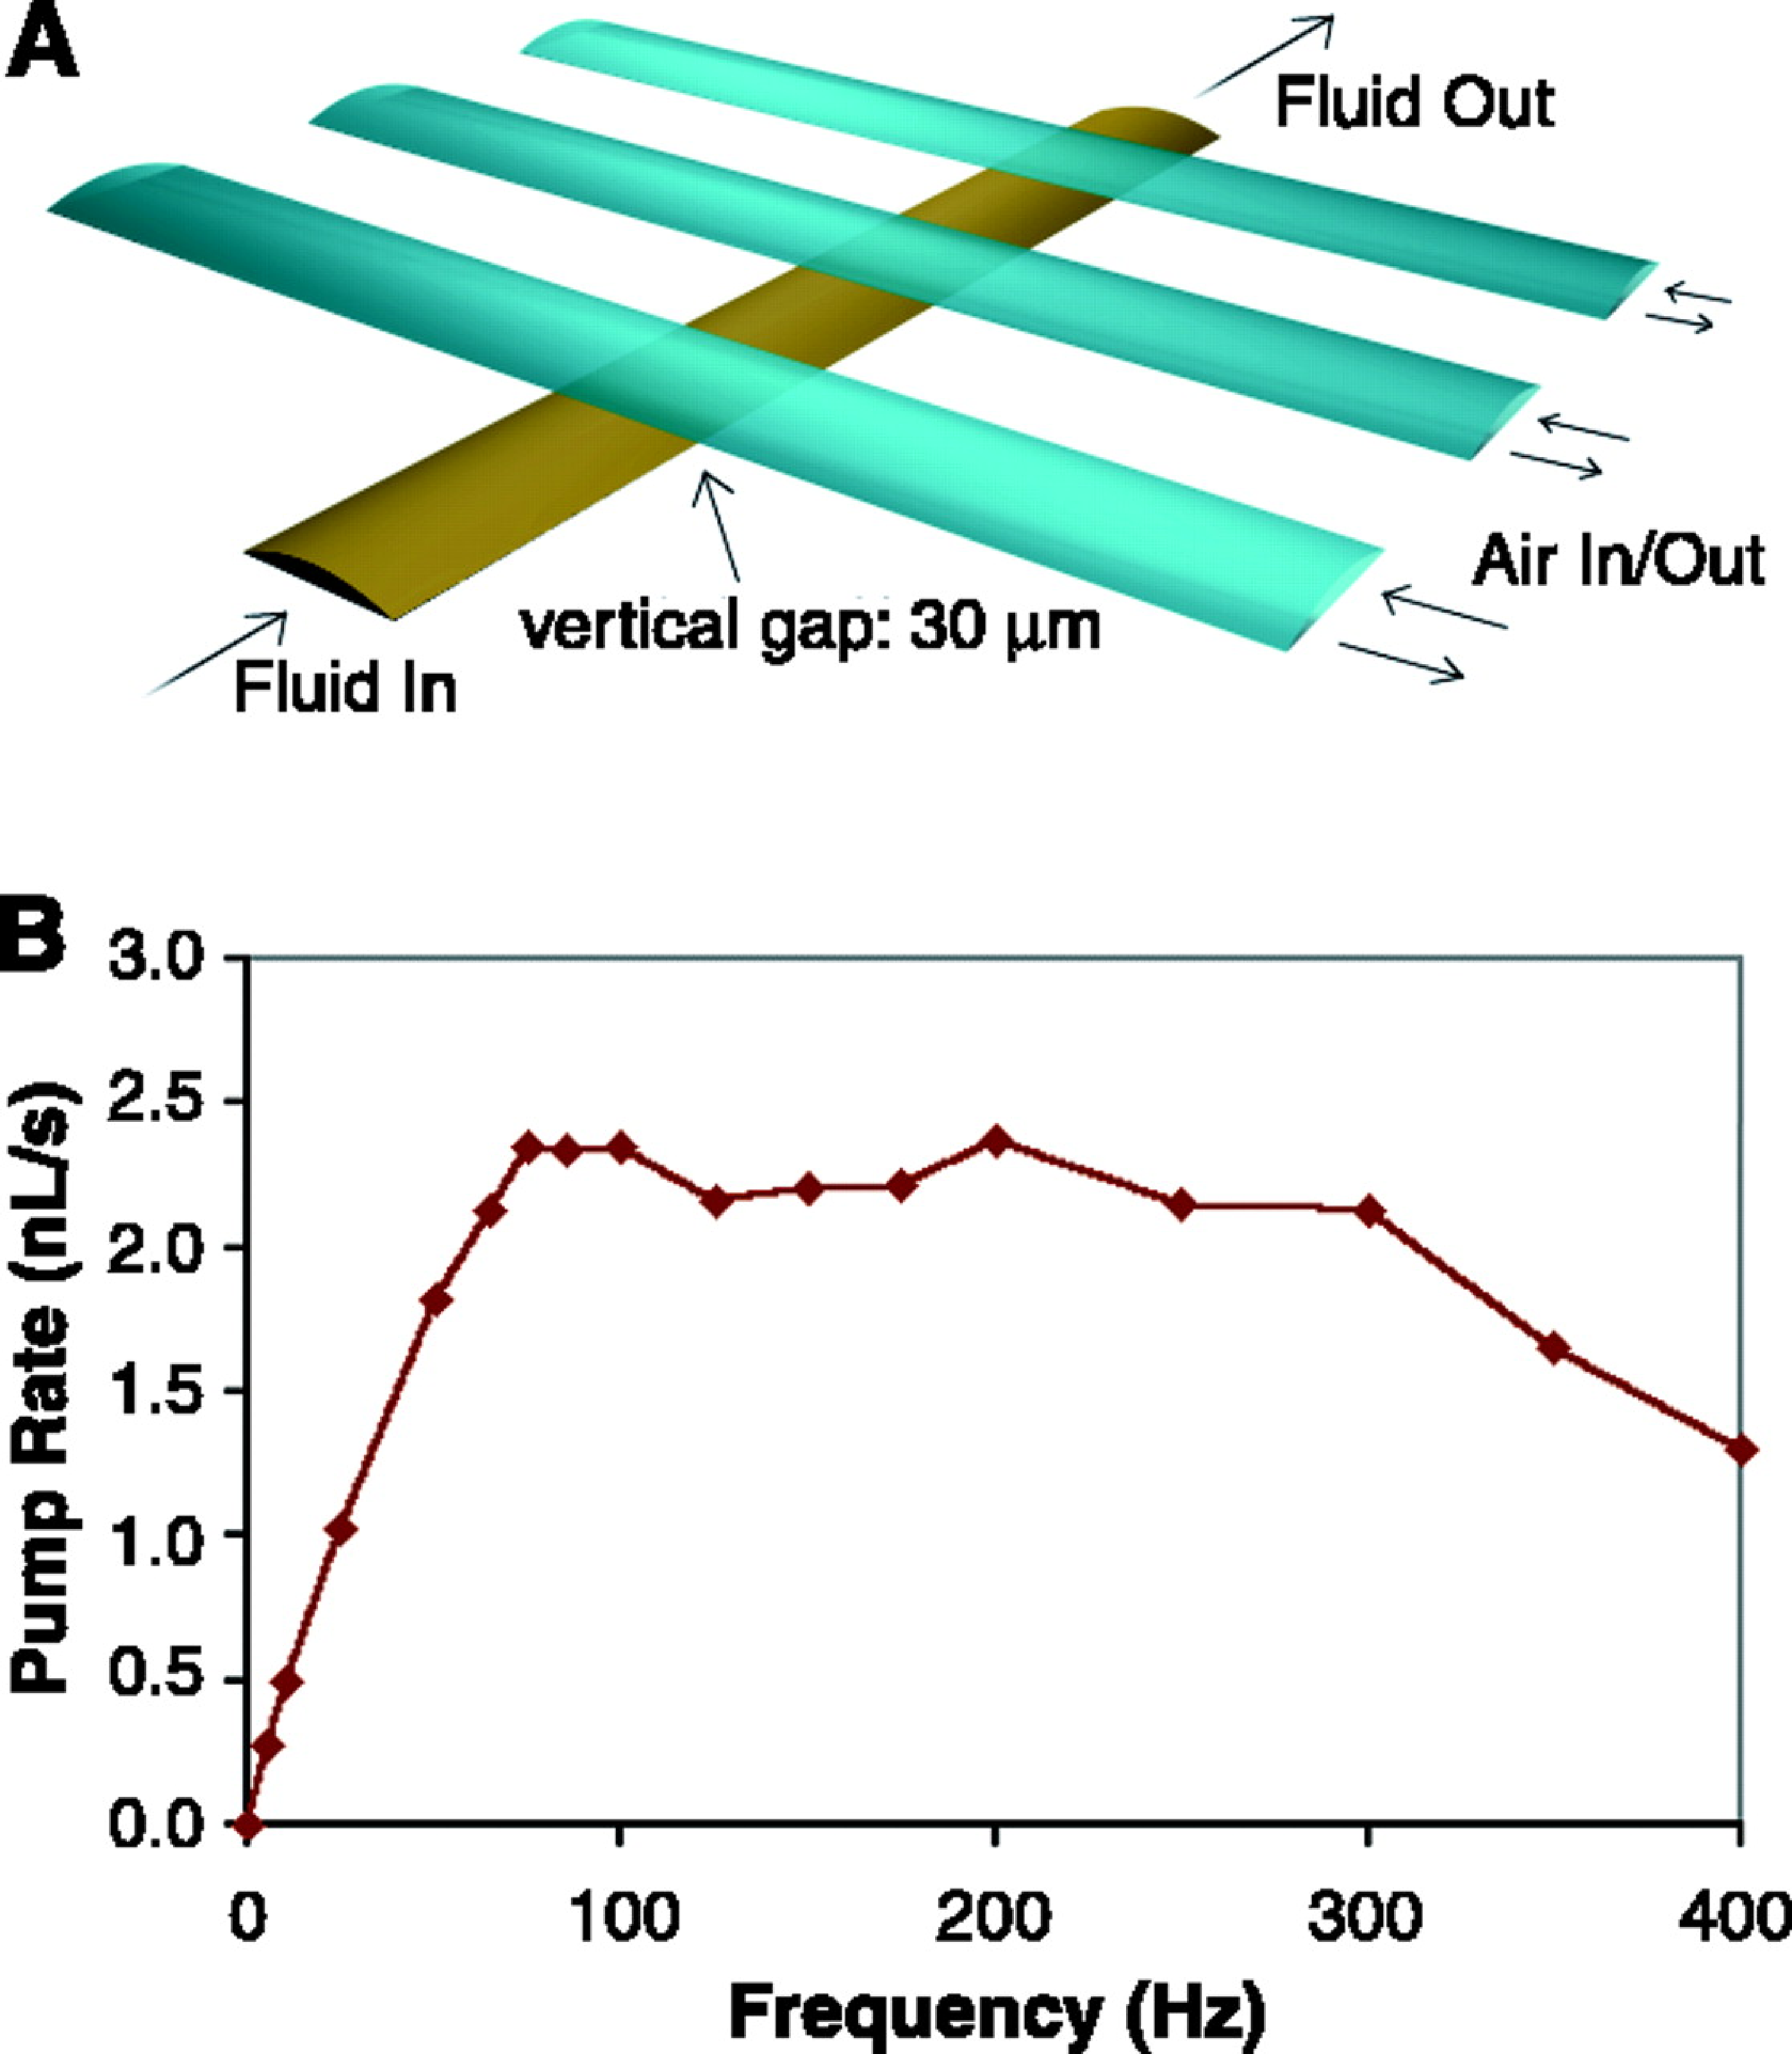
\includegraphics[height=10cm,keepaspectratio]{UngarFig.png}
\end{center}
  \caption{A) A 3D scale diagram of an elastomeric peristaltic pump. The channels are 100 μm wide and 10 μm high.
  Peristalsis was typically actuated by the pattern 101, 100, 110, 010, 011, 001, where 0 and 1 indicate “valve open”
  and “valve closed,” respectively. B) Pumping rate of a peristaltic micropump versus various driving frequencies. This
  figure is reproduced from \citep{RN59}.}
  \label{fig:Ungar}
\end{figure}

Pumps that integrate pumping ‘on chip’ are key to minimising the dead volume within the device.
Unger and co-workers \citep{RN59}, were amongst the first to do this by micro-fabricating PDMS valves
using soft lithography. \fig{fig:Ungar} shows the devices, these work by having a central fluid path that has various gas
channels running perpendicular above it. By simply applying air pressure, the gas channel expands cutting off
the flow in the fluid path beneath. When these valves are actuated in sequence, they produce a
net movement of fluid and flow rates of 2.5 nL/s were achieved.

Leslie et al \citep{RN100} had slightly different
approach. In the ‘pump’ the PDMS forms
a dome above a circular structure in the fluid channel that is the depressed using air
pressure. In order to control the flow they use so called fluidic diodes, these work
analogously with electric diodes, by only allowing fluid flow above a certain pressure in
one direction only. These diodes are formed by having a weir that separates two fluid
channels covered by a compliant PDMS membrane. When the internal fluid pressure reaches the
threshold, this pushes the PDMS membrane up and allows fluid connection over the weir. The
pressure required to open the diode depends on the thickness of the PDMS ceiling and is
predictable which allowed control of flow in the chip at large.

\begin{figure}
\begin{center}
  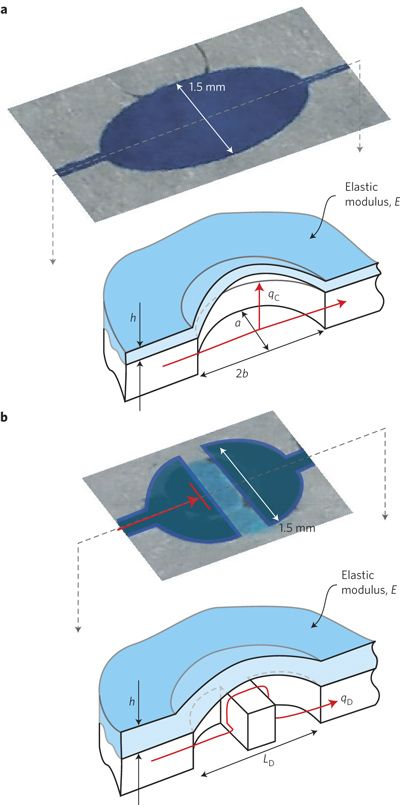
\includegraphics[height=12cm,keepaspectratio]{Leslie-Valves.jpg}
\end{center}
  \caption{\textbf{a}, Discrete fluidic capacitors are created by bonding deformable films (in
   this case, PDMS) over reservoirs placed in the network between fluidic channels (resistors)
    fabricated in glass. These features store and release fluid (volumetric flow rate, qC) in
    proportion to the time rate of change in pressure inside the network; the proportionality
    constant (capacitance, C) depends on film thickness (h), span (a, b) and elastic modulus
    (E). \textbf{b}, Discrete fluidic diodes are created by bonding deformable films around
    weirs that separate two channels in the network. When the internal pressure is larger than
    the external pressure, the diode opens and exhibits nonlinear pressure–flow relationships
    (volumetric flow rate, qD) dictated by solid–fluid coupling. When the internal pressure is
    less than the external pressure, the diode pulls shut and prevents flow. Figure taken from
    \citep{RN100}.}
  \label{fig:Ungar}
\end{figure}

There are specific challenges related to enabling on-chip pumping in a high magnetic field to perform high
resolution NMR spectroscopy. Firstly, the materials used should be compatible with a high
magnetic field clearly ruling out ferrous metals, this also rules out materials that
have a significantly different magnetic susceptibility to that of the chosen fluid (in this
case water). As described in chapter \ref{Chapter:Droplets}, susceptibility mismatches need to be carefully
managed, or they will interfere with the homogeneity of the magnetic field which
essential for production high resolution spectra. Secondly, materials chosen must also be
conducive to rapid prototyping, and as such must be cheap and readily available as well as
be easily cut by a laser cutter and bonded using a simple method. These reasons rule out
glass, a common microfluidic material, which is not easily cut using a standard
laser cutter. Thirdly the chip, when fully assembled, should not be more
that 1 mm in thickness, due to limitations imposed by the strip-line probe geometry \citep{sharma2019modular}. This
limitation  means that more brittle materials, such as glass, would be too fragile for
continuous insertion into the probe and magnet. Lastly,
the device should be able to seal against gas and liquid pressures whilst in operation
inside the magnet.

With all these limitations, poly(dimethylsiloxane) (PDMS) would seem an ideal candidate. It is: cheap and
readily available; easy to cut and bond; and can but made into 1 mm layers to fit the
transmission line probe. However, due to its amorphous structure the $^1$H background
signal is large and broad across the range of ppm that the signals that we are interested in
appear. This broad background signal makes it impractical to suppress and any suppression would also suppress the
signals that we are interested in, and could lead to difficulties in quantification of
substances present in the sample under investigation.

In the design shown, a PDMS layer is still used. However, it is removed from the
sensitive area around the sample chamber so that it does not interfere with the signal
collected from the device. The 3D printed parts role here is three-fold, firstly, it acts
as a conduit for delivering liquids and transporting them around the device. Secondly, it
allows for the pressurised air to be delivered which drives the pneumatic valves and
enables pumping. Lastly, when screwed together, the 3D printed parts form a seal against
liquid and gas leaks.

Nuclear magnetic resonance (NMR) is an ideal tool with which to study live systems,
which owing to its non invasive non destructive nature, can give insight into living
systems \textit{in situ} and allows for longitudinal studies of them. However, in order to
keep these systems alive, and truly replicate \textit{in vivo} conditions, they need fresh supplies of oxygen and nutrients. One way of achieving this is by perfusion of
liquid that has been exposed to fresh supplies of oxygen. Perfusion can be accomplished by
pumping liquid through the microfluidic device and then out to a reservoir that is in
contact with a supply of oxygen. This method would, however, dilute any metabolites
given off by the living system that is under investigation within the device, and
since the biggest limitation of NMR is sensitivity, it is pertinent to avoid this. This
means that the pump would ideally be integral to the device itself. This could reduce the
overall volume of the system to tens of microlitres which is much better than the tens of
millilitres that come from having an external pumping network. This means that the pump
would ideally be integral to the device itself.

In summary, the device must meet the following criteria:
\begin{itemize}
  \item Non-magnetic parts where possible, susceptibility matched.
  \item Easily fabricated using rapid prototyping.
  \item Low dead volume.
  \item Biocompatible.
  \item Geometry compatible with transmission line probe.
  \item Easily assembled and operated \textit{in situ}.
\end{itemize}

The solution employed here involves a multilayered PMMA device,
with two PDMS membranes, sandwiched between two 3D printed holders held together with brass
screws. The PMMA device houses the structures for the valves, as well as the fluid circuits,
including an NMR sensitive sample chamber and on-chip reservoir. The PDMS layers have two
separate functions, the top membrane forms the valves with the PMMA structures whilst the
bottom membrane acts as an o-ring to seal against fluid leaks. The 3D printed holders
are also multi purpose. The top holder forms the last part of the valves by sealing the
PDMS-PMMA valve and allowing the delivery of pneumatic pressure through the bore of the
magnet to the device. The bottom 3D printed holder allows the device to be filled and
supplies external ports for fluid short circuiting. Together, they help seal the device
against gas and liquid leaks. This device coupled with a bespoke, homebuilt probe enables
pumping and observation by NMR in a microfluidic device.

\subsection{Materials and Methods}

The devices are composed of three layers of cell cast poly(methyl methacrylate) (PMMA,
Weatherall Equipment). The sheet thickness was 200 $\mu$m for the top and bottom layers, and 500 $\mu$m for
the middle layer. The channels and sample chambers were designed in
AutoCAD and cut using a CO$_2$ laser (HPC Laser ltd.) to an approximate width and depth
of 150 $\mu$m. These layers were bonded together using plasticiser (2.5\% v/v dibutyl
phthalate in isopropyl alcohol) and subjected to heat and pressure (358 K, 18.6 MPa).
To seal the devices, two polydimethyl siloxane (PDMS, Shielding Solutions) were
designed in AutoCAD and cut using the same laser as the PMMA layers.

The PMMA and PDMS were screwed together and held in place using 3D printed devices
designed in SolidWorks (Acura Xtreme, ProtoLabs). These, as shown in \fig{fig:3Ddevice}, seal the
device whilst enabling the filling of the device as well as delivering the pressurised
air for the peristaltic pumping.

The hardware for controlling pumping comprised of a solenoid valve system with 8
individual valves (Festo, RS). These were connected to 3mm plastic tubes (Festo, RS)
and all supplied from an in-lab air pressure source. This valve system was connected,
via a solderless breadboard, to an arduino (Mega 2560, RS) controller allowing for
individual control of each of the valves. The Solenoid valve system was powered using
a 24V supply.

The device was put into a transmission line based home-built probe. In this, the
device is held between two striplines with the inner sample chamber lining up with the
constriction on the strip-lines. NMR measurements were performed on a bruker AVANCE
III spectrometer and 11.7 T magnet. Spectra were collected using 64 scans using a 90
degree pulse length of 2.5 us at 50 W of power. Water suppression was achieved by
using presaturation with $5x10^{-4}$ W.

100mM solutions of sodium acetate (Merck) and 3-(Trimethylsilyl)-1-propanesulfonic
acid (DSS, Merck) by dissolving 82 mg and 196 mg in 10 ml of deionised water
(ReAgent)
respectively. The two fluidic loops were then filled with these separately and the
in/out ports short circuited.

Firmware for controlling the peristaltic pump was written in Arduino and is provided in the appendix.
This has the ability to put the pump into 3 states
“advance”, “mixing” and “quiet”. The “advance” state pumps from the outside loop of
the device to the inside loop for a desired number of seconds; “mix” pumps around the
inner loop for a desired number of seconds; and “quiet” stops all pumping and leaves
all valves open indefinitely.

\begin{figure}[h]
  \begin{center}
  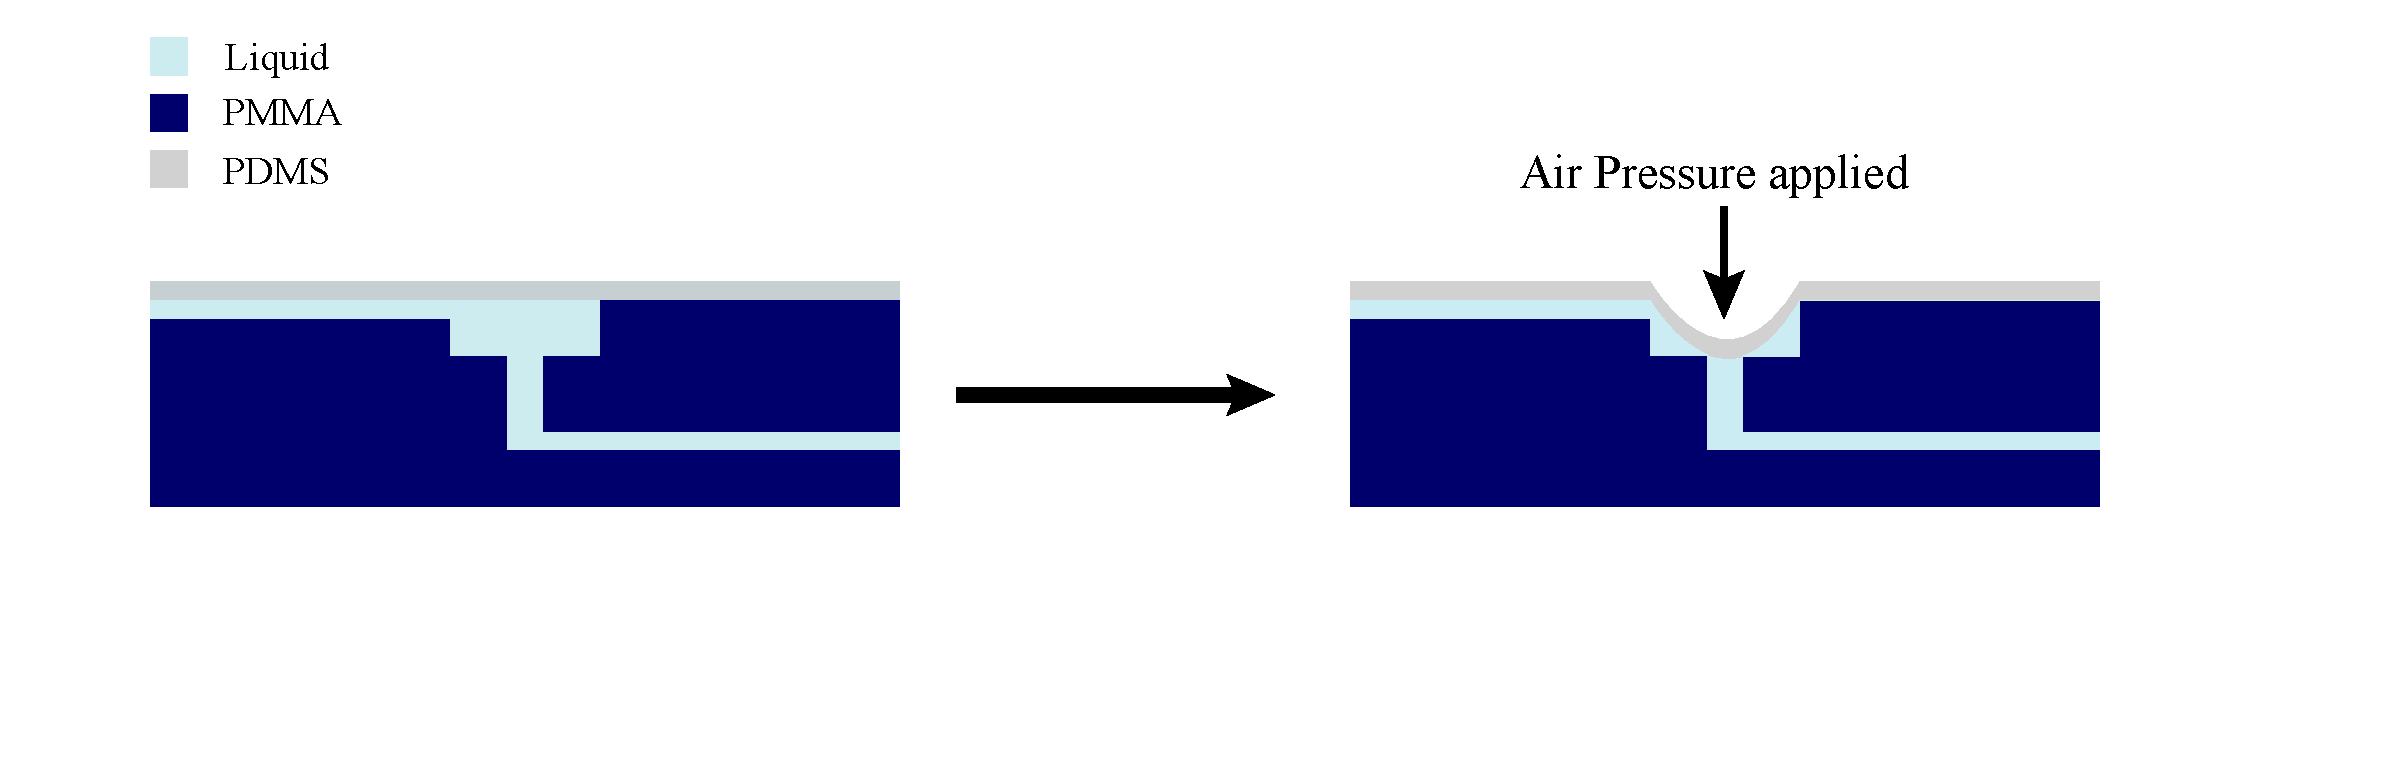
\includegraphics[width=\columnwidth]{Peristaltic-principle.pdf}
  \caption{A cut-through view of the valves in the device showing how when air pressure is
  appplied the PDMS membrane is pushed down and seals the small hole cut in the middle layer.}
  \label{fig:PP-device}
  \end{center}
\end{figure}

\begin{figure}[h]
  \begin{center}
  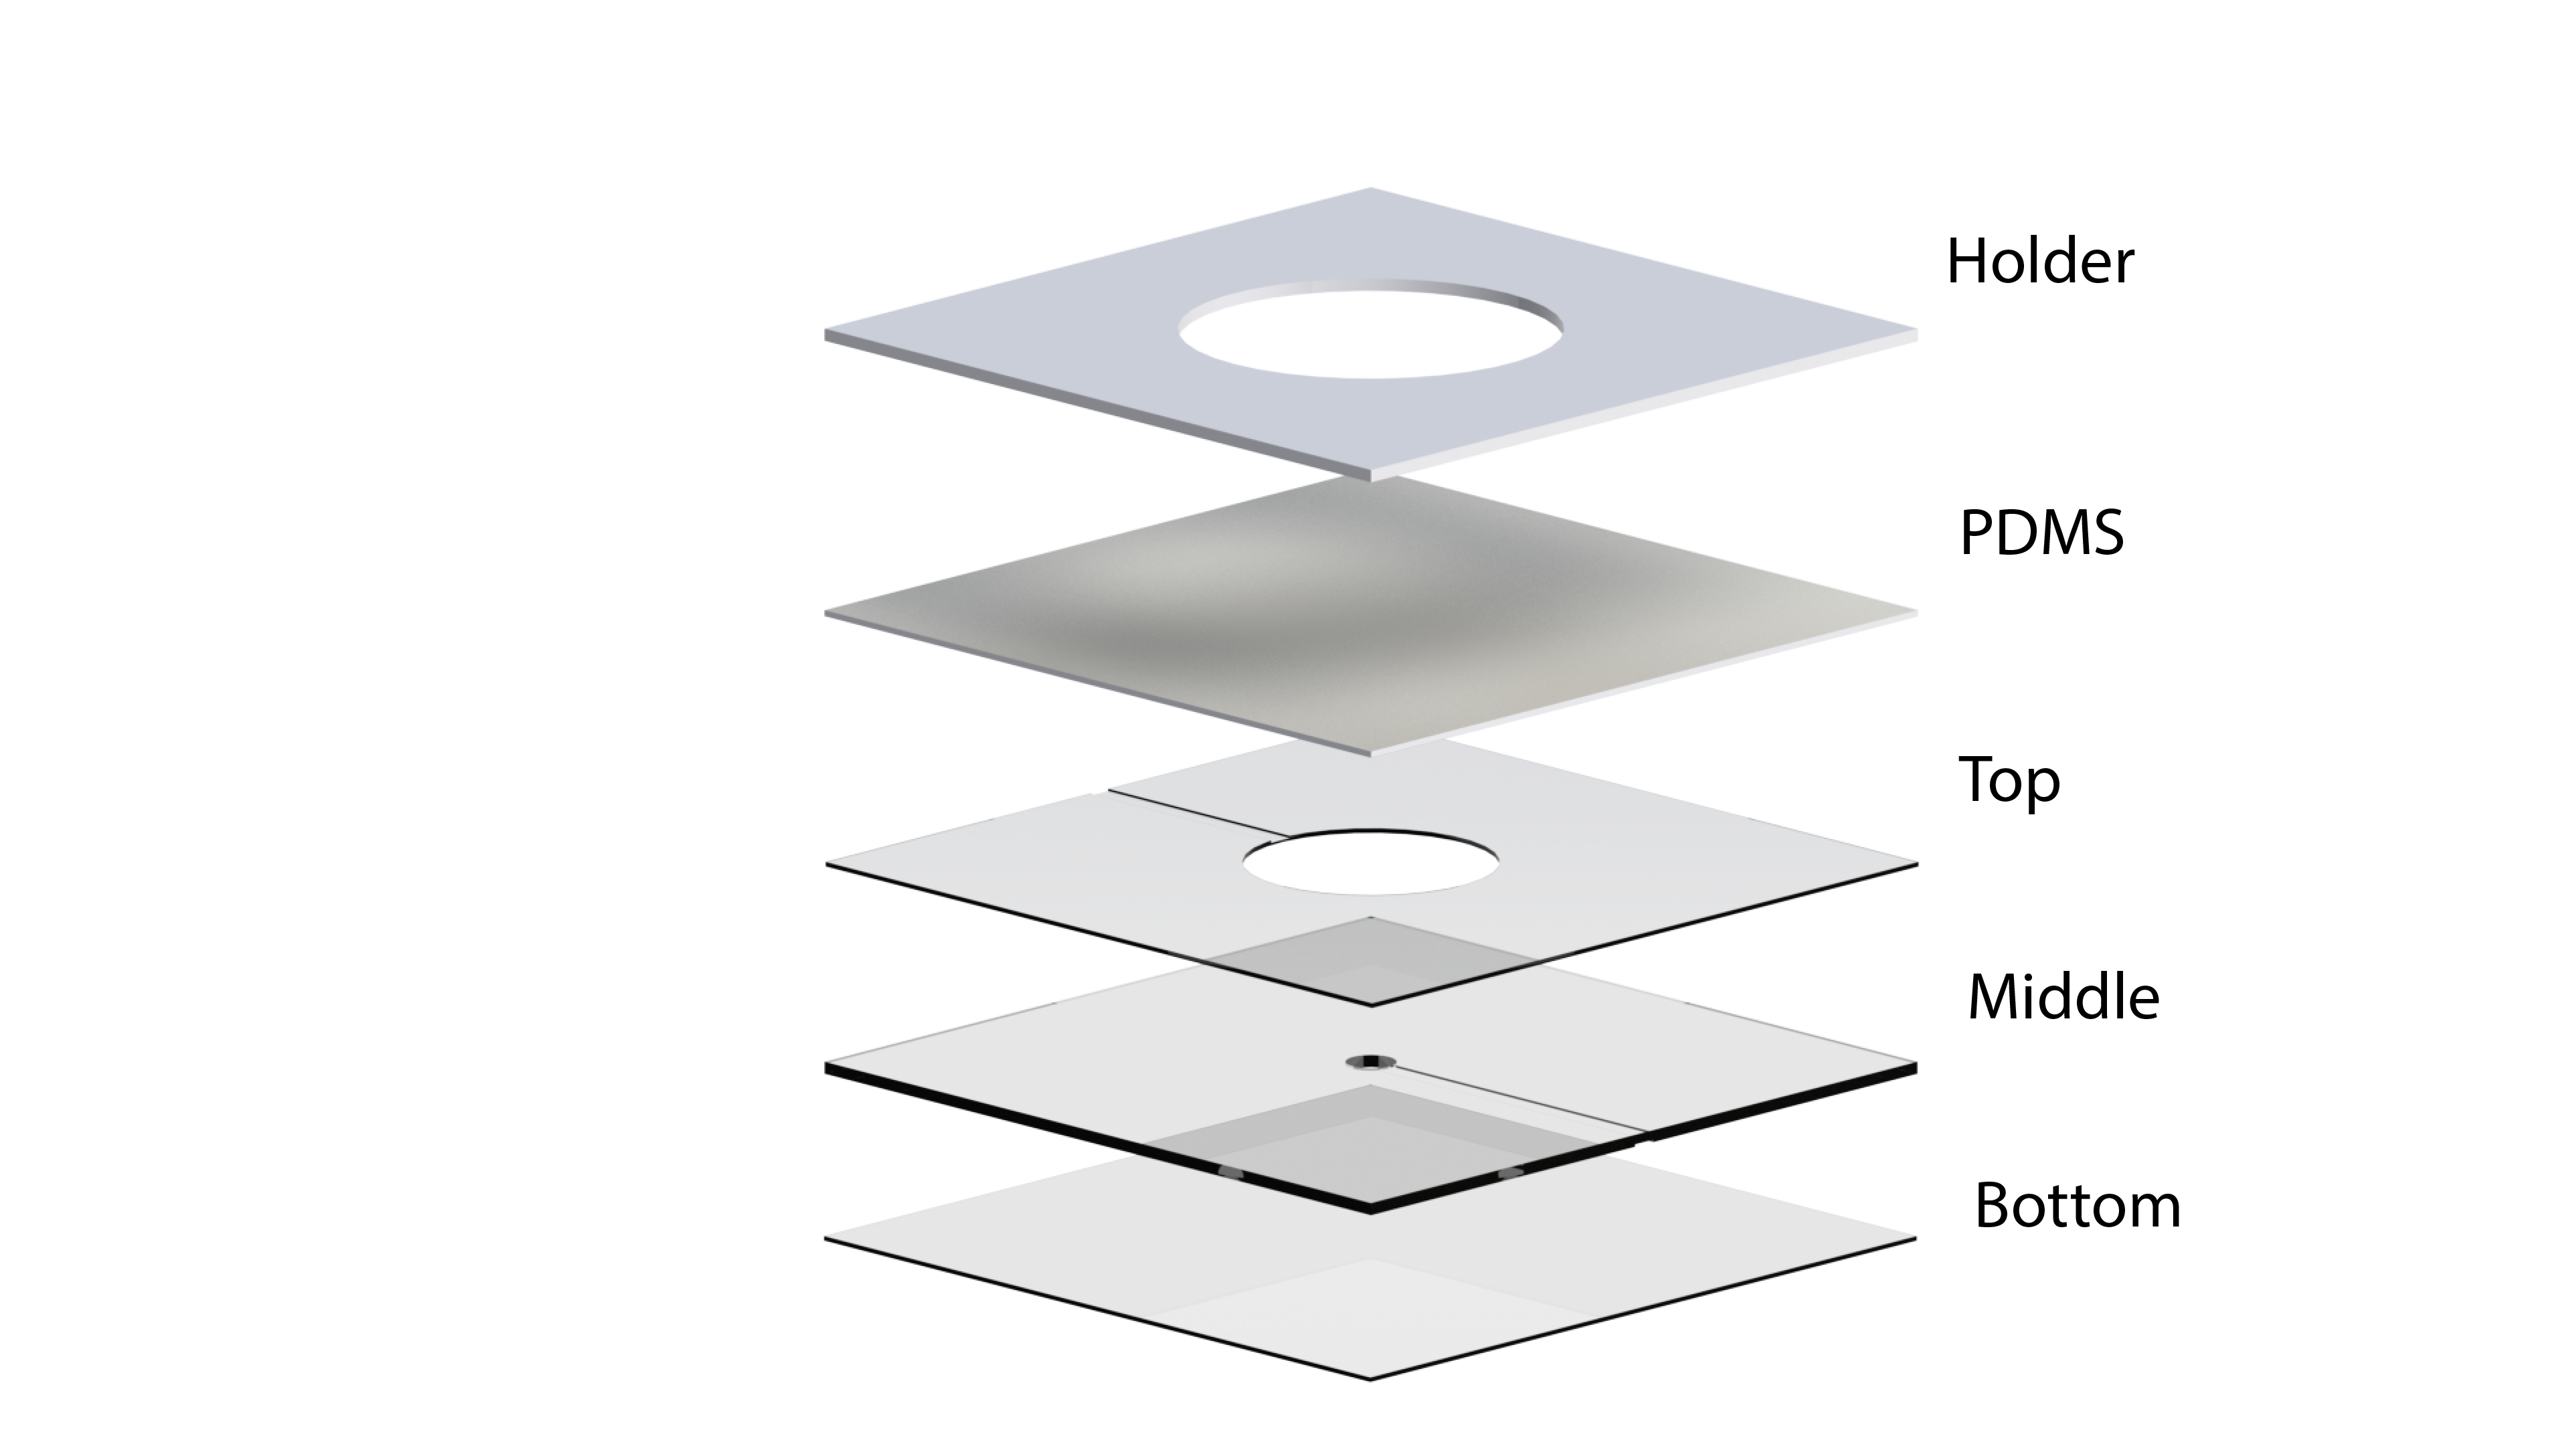
\includegraphics[width=\columnwidth]{3DRenderOfValve-01.png}
  \caption{3D render of a single valve with 3D printed layer shown too}
  \label{fig:ValveRend}
  \end{center}
\end{figure}

\section{Results and Discussion}

\subsection{Peristaltics}

In order for the dead volume in the device to be kept at a minimum, the valves are implemented
in the fluid path on the device itself. Shown below in \fig{fig:PP-device} is the
basic principle behind the design.

\begin{figure}[h]
  \begin{center}
  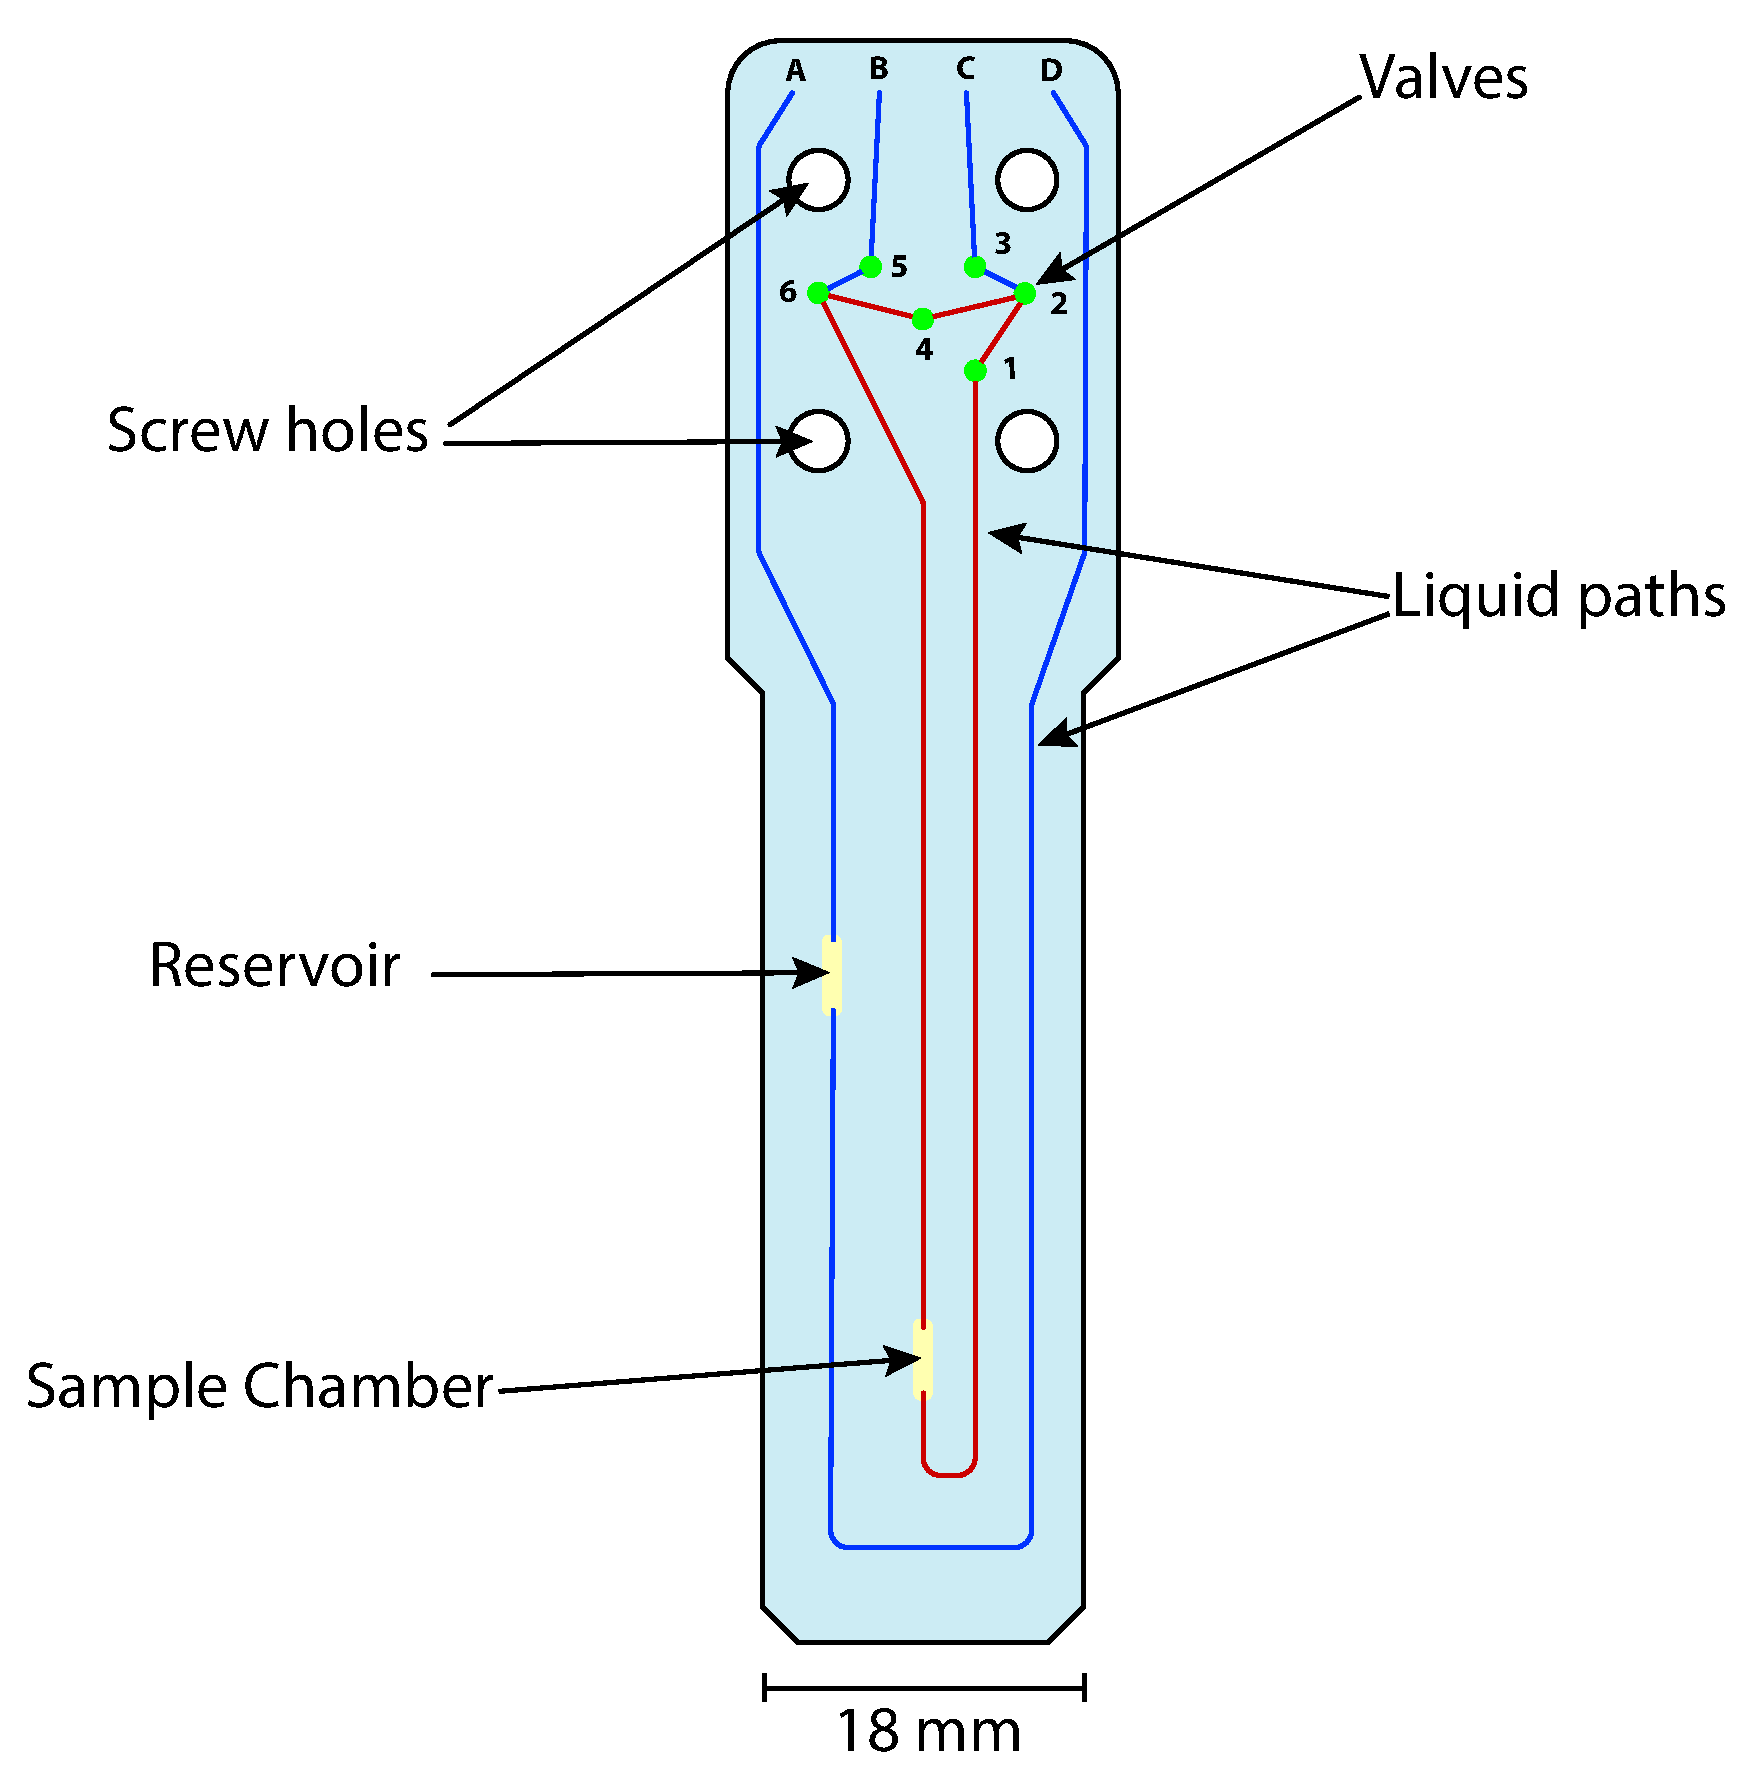
\includegraphics[width=\columnwidth]{Experimental-chip.pdf}
  \caption{A CAD drawing of the chip designed for pumping and mixing. Inner (red) and outer (blue) liquid circuits; liquid ports (\textbf{A}-\textbf{D}) and valve positions (1-6) shown.}
  \label{fig:Chip}
  \end{center}
\end{figure}

In the device, there are valves cut into the layers of PMMA. These are formed by two holes
in the top and middle layer. The hole in top layer has a radius of $500 \mu m$ whilst the
hole in the middle layer has a radius of $100 \mu m$. The top layer has a channel (approx.
$150\mu m$ in width and depth) scored into it to deliver fluid to the top chamber whilst
the middle layer
has a similar channel scored on the under-side to carry fluid away. When covering the hard
PMMA structure with the more compliant PDMS membrane of $250 \mu m$ thickness, applying
air pressure from above seals the valve by covering the hole in the middle layer.

\begin{figure}[h]
  \begin{center}
  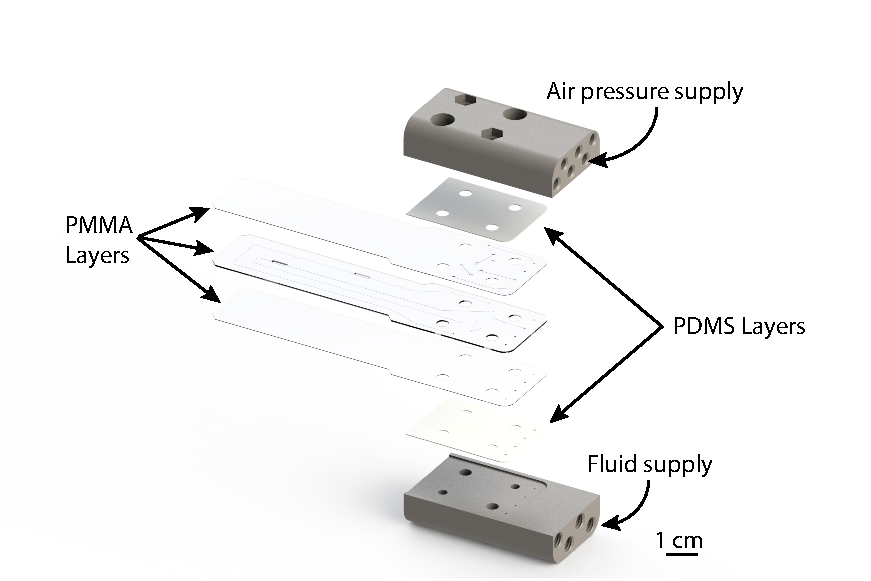
\includegraphics[width=\columnwidth]{Peristaltic-Chip-Render-01.pdf}
  \caption{A 3D representation of the device with separate layers of chips and PDMS
  layers shown.}
  \label{fig:3Ddevice}
  \end{center}
\end{figure}

A 3D rendering of a single valve is shown in \fig{fig:ValveRend} and shows the ratio of pump holder opening, top hole; and middle hole respecively. The key to these valves
is that the scored channels are on opposing sides of the valve.

\begin{figure}[h]
  \begin{center}
  \includegraphics[width=\columnwidth]{Micrographs-02.png}
  \caption{Micrographs of A: free chip showing two valves B: An assembled device with an
  open valve C: An assembled device with a closed valve, the arrows indicate the area where the PDMS is
  in contact with the PMMA and is sealing the hole.}
  \label{fig:Micrographs}
  \end{center}
\end{figure}


In \fig{fig:Micrographs}, micrographs of the chip outside the holders are shown with the valves
where one can see the fluid channels on opposing side of their respective layers. Also given,
is side by side comparison of the same valve (valve 2 in \fig{fig:Chip}) open (2) and closed
(3) one can see the 'ring' formed by the PDMS as it seals against the middle layer.

In my design, there are 6 such valves all individually addressable with air pressure, which when
coupled with home-written Arduino firmware, can be actuated in sequence in order to move
fluid in a given direction. The block diagram of the arduino set-up is shown in
\fig{fig:ValveSetup}. By varying the frequency and lambda parameters, listed in the
firmware, one can control the liquid pumped in a given time.

\begin{figure}[h]
  \begin{center}
  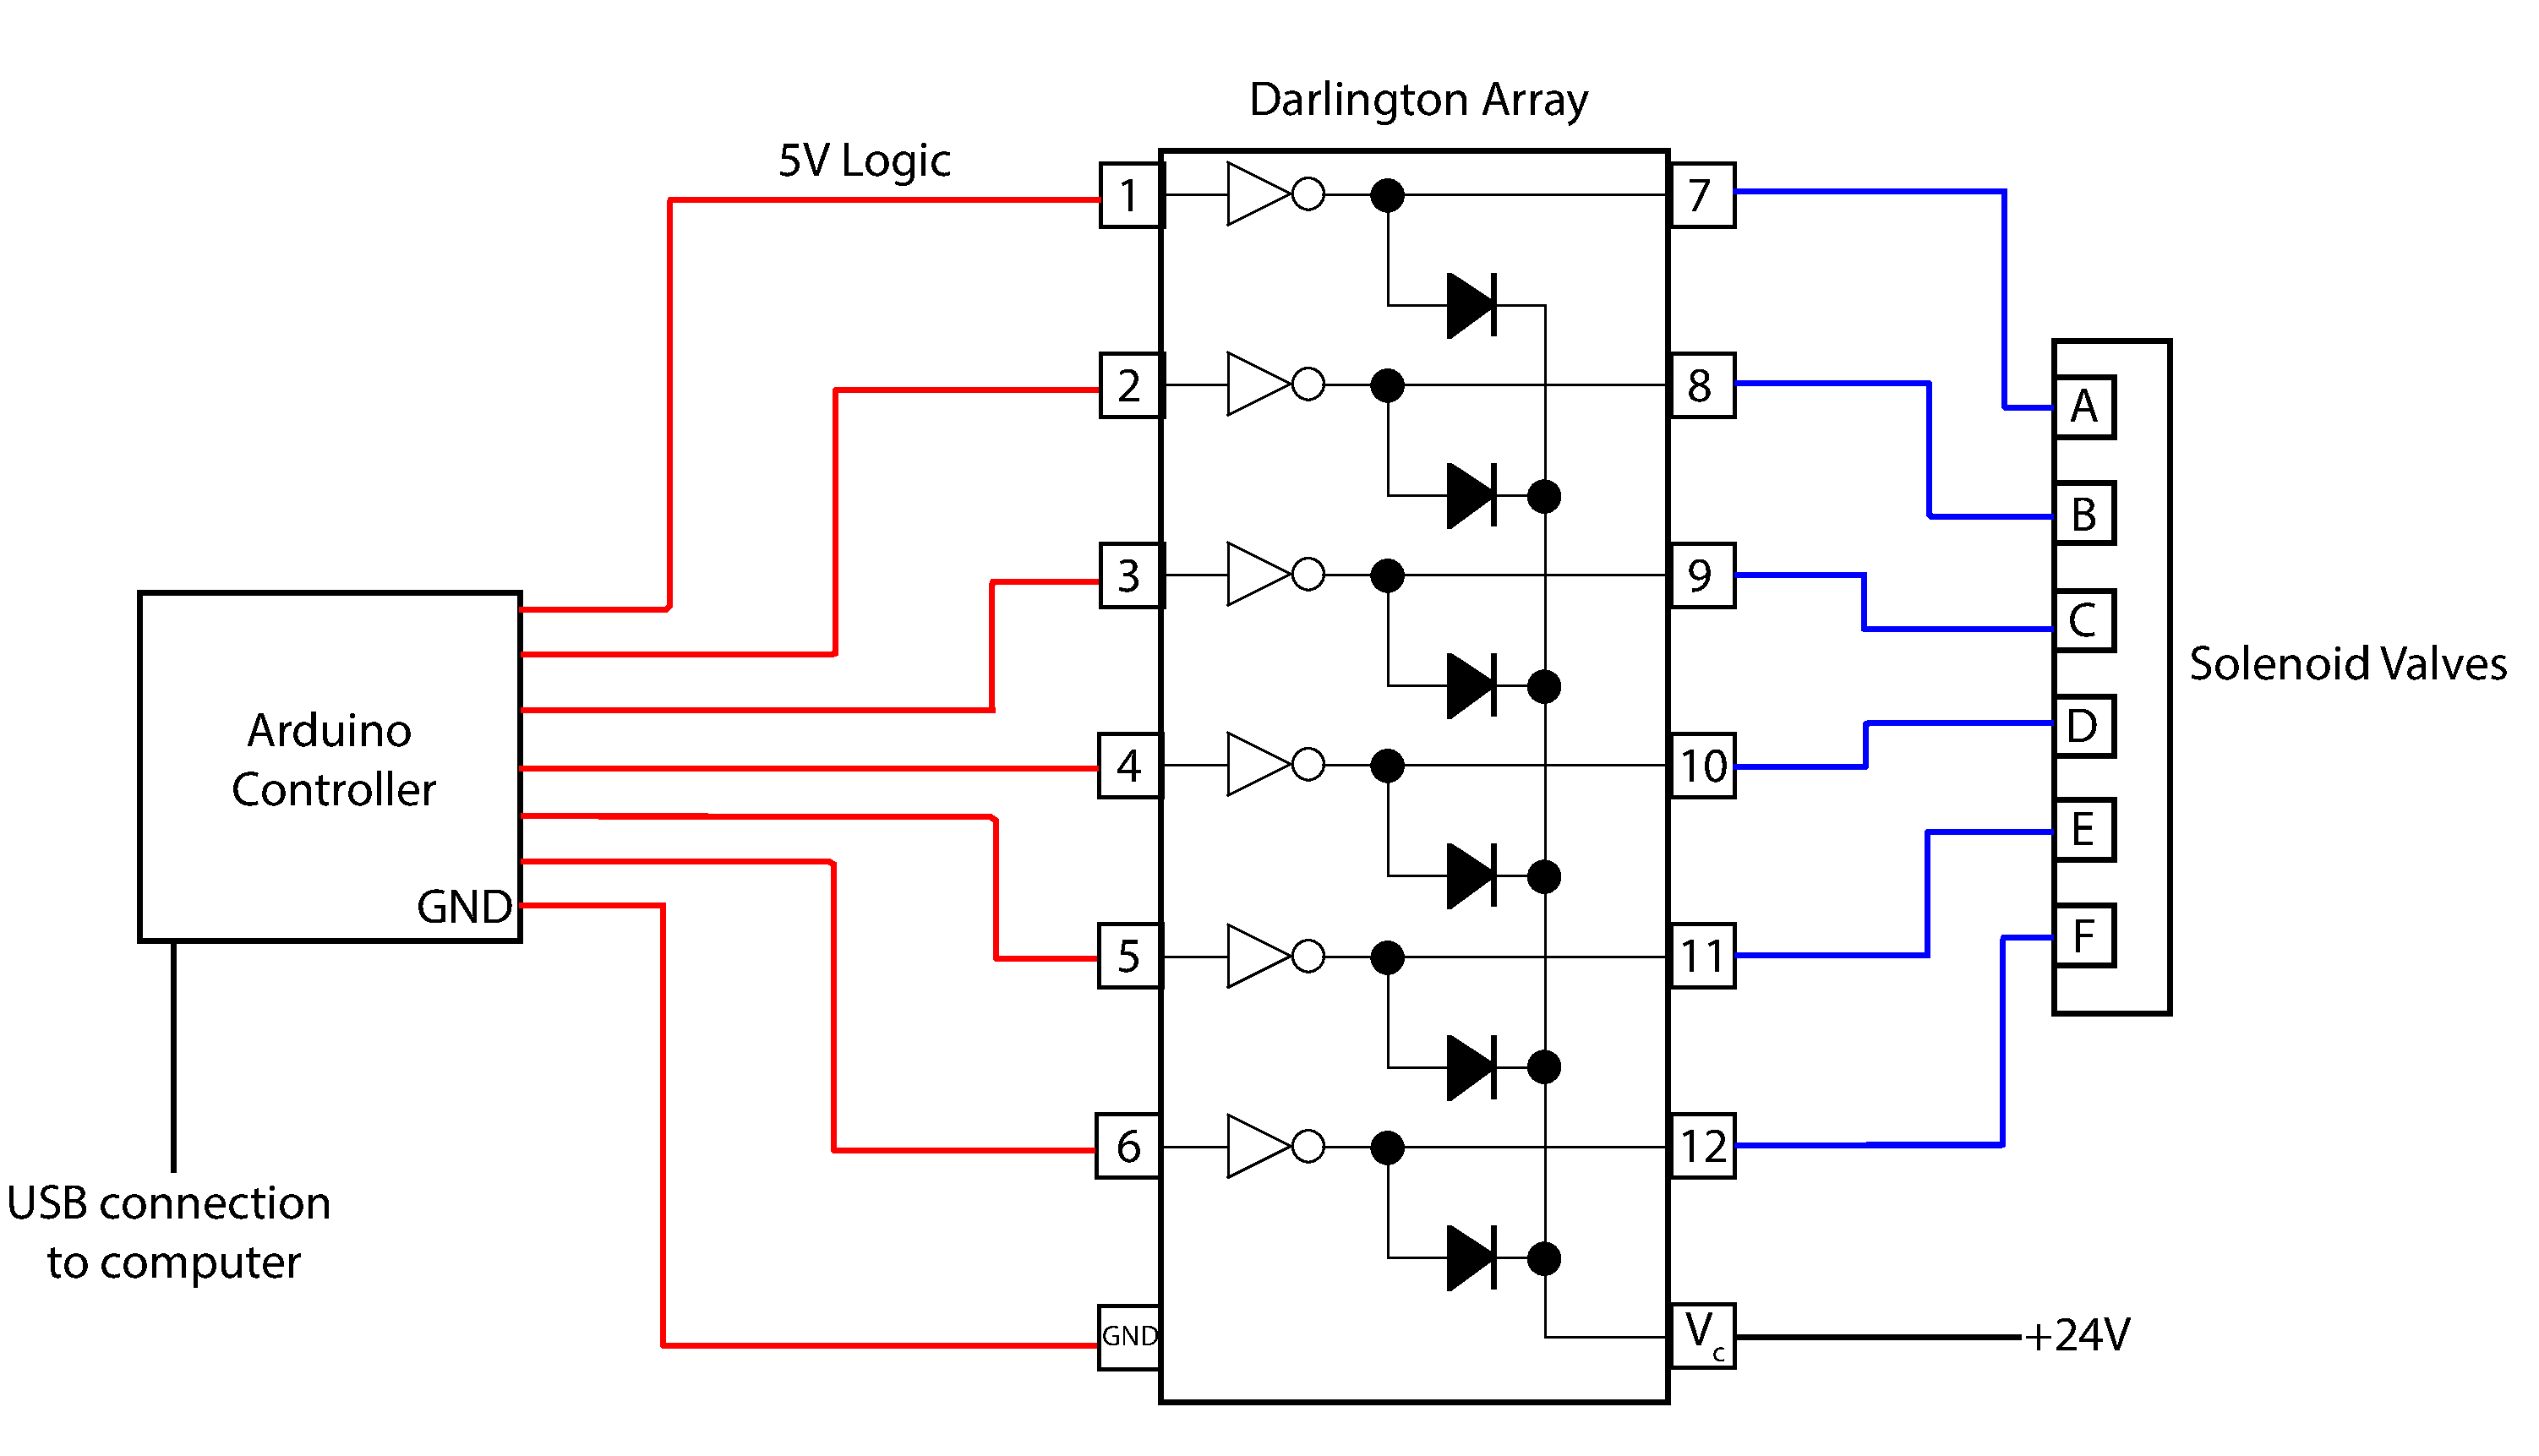
\includegraphics[width=\columnwidth]{Arduino-Valve.pdf}
  \end{center}
  \caption{An arduino controller is connected to, and powered by, a laptop via USB. The controller is connected
  to a darlington array via six 5V logic connections (shown in red) when addressed, these allow the corresponding pin
  opposite to draw power from the +24V connected from an outside source. The blue lines indicate the the wires
  carrying 24V to the solenoid bank which are pneumatically connected to the valves in the chip as labelled. }
  \label{fig:ValveSetup}
\end{figure}

As well as 6 valves, the chips also have two separate liquid
circuits that can be connected externally by attaching tubes to the top of the 3D
holders as shown in \fig{fig:Chip}. The inner circuit on
the diagram contains the pumping network which can be
modified to pump around the internal circuit or the complete network, and an NMR
sensitive sample chamber where measurements are performed. The external circuit,
contains an identical sample chamber that helps to keep the relative
volumes of the two circuits similar. The chip is filled from the
‘bottom’ using the 4 small access holes at the top of the chip (\textbf{A}-\textbf{D}).
This then allows the valve network and pressurised air to be
on the top side of the chip. The challenge in the chip was to fit
all the liquid paths and valve network around the 4 large
holes in the top of the design which accommodate the screws
necessary to hold the device together, and seal against leaks of
both liquid and gas.


\subsection{Characterisation of flow}

Characterisation of flow experiments where performed with the device in an “open”
configuration. This means that after the device was screwed together the two circuits shown
in blue and red were joined together by fixing tubing between the \textbf{A} and \textbf{B} ports shown in
\fig{fig:Chip}. This leaves \textbf{C} as the “in” port and \textbf{D} to be the “out” port with valves 3, 2, and 1
being actuated in sequence to pump, and valve 4 sealed.

The device was connected to translucent polytetrafluoroethylene (PTFE) tubing (Outer
diameter 1.6 mm, inner diameter 0.8 mm) with one end submerged in a 500 mL beaker
containing filtered DI water (Reagent). Next to the device a ruler was secured to the bench
top with the tubing fixed parallel to it. The pump was then switched on and the device
allowed to draw water, and pump out the other side. When the water meniscus reached the tubing
next to the ruler a timer was started and the distance along the ruler was recorded every
minute for 10 minutes. The was repeated 3 times for frequencies from 0.25-1 keeping the
lambda constant at 3, which had shown through trial and error to be the optimum number.

The graph shown in \fig{fig:Graph} is the result of plotting the cumulative volume pumped
vs. time. All 4 frequencies show very little deviation from linearity in the
long term and also show very small error bars (plotted as ±2$\sigma$).

\begin{figure}[h]
  \begin{center}
  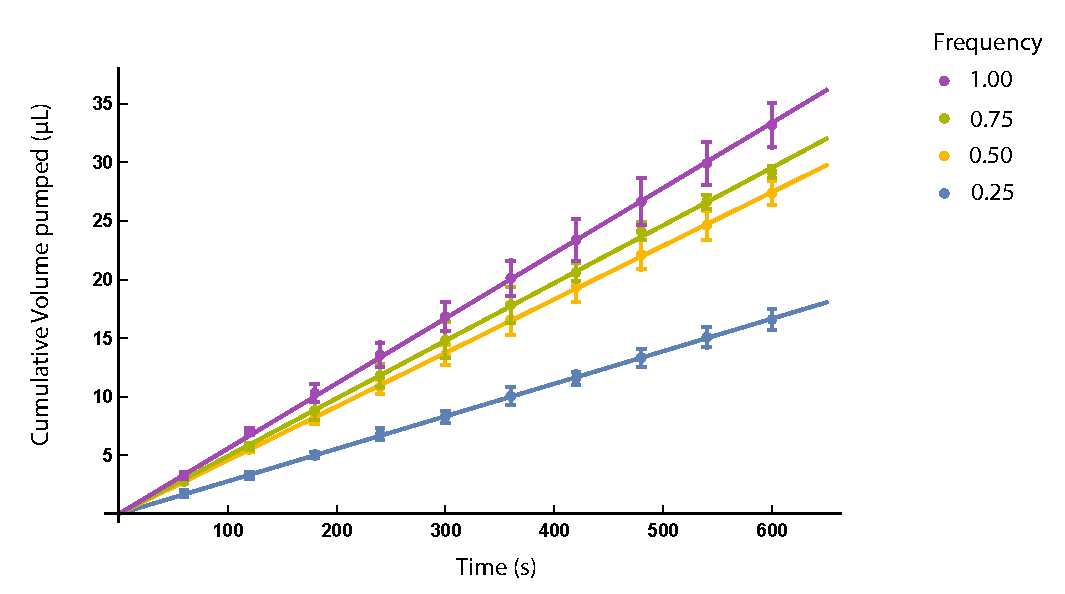
\includegraphics[width=\columnwidth]{ALLPlots.pdf}
  \caption{Plot of the total volume pumped vs time for a chip in the open
  configuration.}
  \label{fig:Graph}
  \end{center}
\end{figure}

\begin{figure}[h]
  \begin{center}
  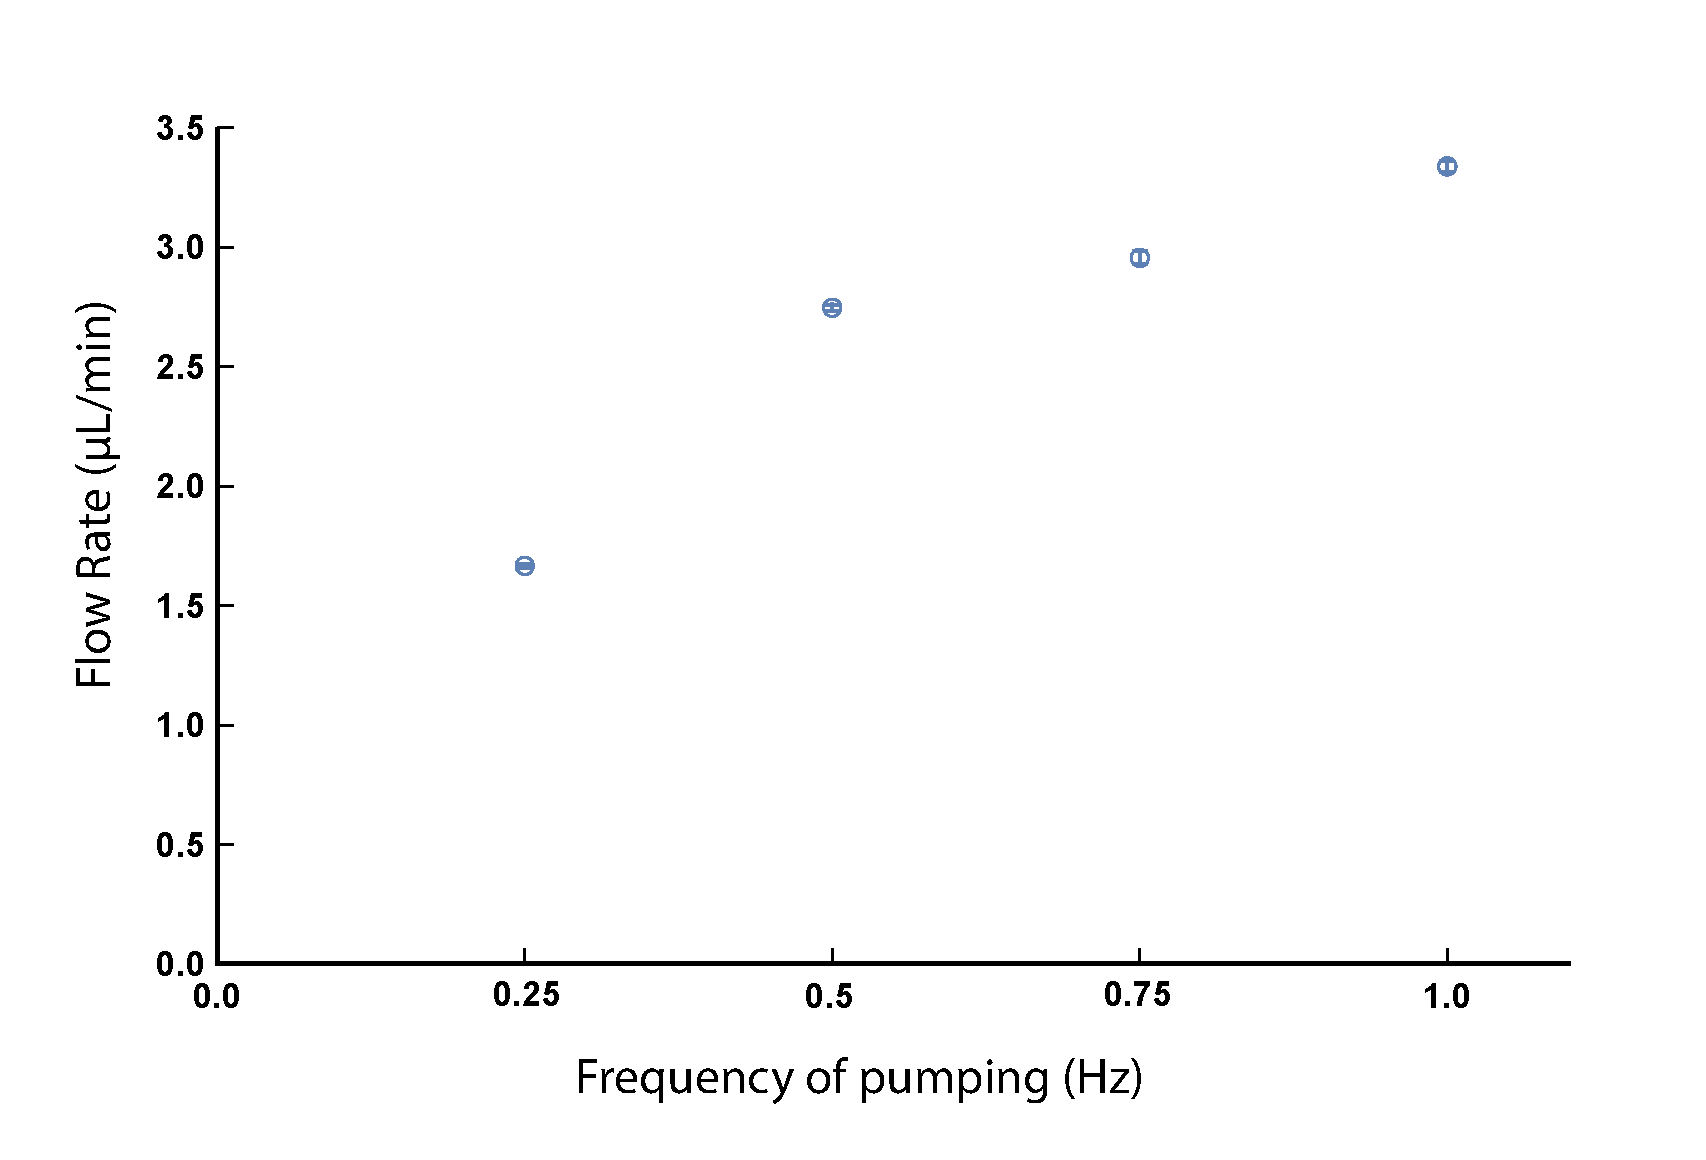
\includegraphics[height=8cm,keepaspectratio]{Flowratevsfreq.pdf}
  \caption{Flow rates produced by the pump at different frequencies.}
  \label{fig:FRvFGraph}
  \end{center}
\end{figure}

In \fig{fig:FRvFGraph}, the flow rate of the pump at varying frequencies is plotted. This
shows that the flow rate doesn't linearly depend on frequency, and seems to level off at higher
frequencies. When initially observing the gradient of the lines in \fig{fig:Graph}, the non-
linearity was attributed to inconsistencies in the tightening of the screws in the device.
However, the small error bars associated with the flow rates across three separate
experiments, each with at least one disassembly and reassembly of the device, it is now thought that the limit of the
pump rate is related to the elasticity of the membrane, and how fast it's able to 'snap
back' and re prime itself to pump in each valve.

\subsection{\textit{In situ} operation of the device}

\begin{figure}[h]
  \begin{center}
  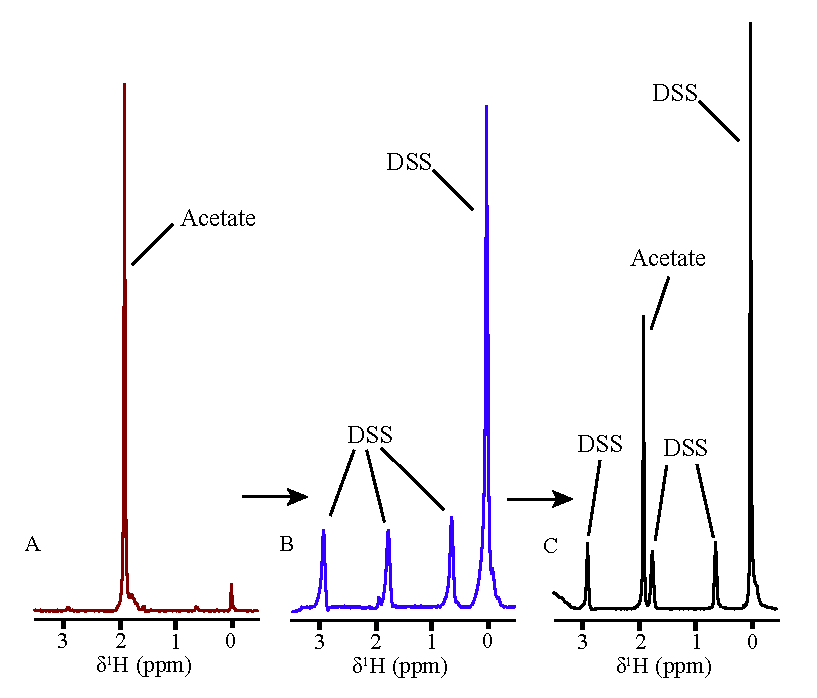
\includegraphics[height=12cm,keepaspectratio]{Acetate-DSS-stackplot-edit.pdf}
  \caption{NMR spectra recorded with 16 transients on a device containing 100mM Sodium
  acetate in the inner circuit and 100mM DSS in the outer circuit.}
  \label{fig:spectra}
  \end{center}
\end{figure}

In order to validate the pumps compatibility with NMR, the device was placed into a home
built transmission line probe inside a 500 MHz magnet. The arduino controller and solenoid valve
bank where secured outside the magnet and the 6 pressurised air lines fed in through the top of
the magnet. The device was then filled with 100mM sodium acetate in DI water (Sigma Aldrich) in
the inner circuit by attaching a syringe to inlet \textbf{B} in \fig{fig:Chip}. 100mM DSS in DI
water (Sigma Aldrich) was added to the outer circuit by syringing into inlet \textbf{A}. The sample chamber then contained only sodium acetate and all the initial signal should arise from this. The two fluid networks
were then connected using two short lengths of 1/16" outer diameter PTFE tubing by joining
\textbf{A} to \textbf{B} and \textbf{C} to \textbf{D}.

First, a spectra was collected of the chip after filling, A in \fig{fig:spectra}, using 16
transients and shows mainly the acetate signal at 1.9 ppm. The pump was then put into
the 'advance' state for 120 seconds which mean the valves are actuated in order to pump
liquid around both circuits. The pump then mixed in the inner circuit for 120 seconds
and a second spectra was recorded, B. This shows the 4 signals typical of DSS at 2.91
ppm, 1.75 ppm, 0.63 ppm and 0 ppm and very little acetate signal. Indicating that the
volume inside the NMR sensitive area has been almost entirely exchanged. Lastly the
pump again advanced and mixed for the same time as before producing the spectra shown
in C. Again, this spectrum is different. It shows all signals expected in abundance.
This points to mixing of the two substances facilitated by the peristaltic pump and serves
as proof, at least in principle, that an NMR compatible microfluidic peristaltic pump
capable of mixing liquids in a controllable manor has been presented here.

\section{Conclusions}

In conclusion, an NMR compatible; low dead volume microfluidic pump has been designed and
manufactured that works inside the bore of a high field magnet. The pump has shown
excellent linearity and stability in the long term as well as performing exchange, and
mixing, of two substances within the device inside a high field magnet. The present limitations
are that precise volume control has not yet been achieved. This is, however, thought to be linked
with the varied tightening of the screws of the 3D holder as well as the presence of bubbles
within the device. Another element that requires further probing is the non-linear dependence of
flow rate on frequency. My intuition is that this depends on the thickness of the PDMS layer
used
however further experimentation with varying thicknesses is needed. Potential future
applications
of this pump include: microfluidic protein binding experiments; \textit{in situ} liver slice
culture and metabolomics; and hyperpolarization experiments.

%%% ----------------------------------------------------------------
%% Conclusions.tex
%% ---------------------------------------------------------------- 
\chapter{Conclusions} \label{Chapter: Conclusions}
It works.

%\appendix
%

\chapter{Appendix} \label{Chapter:Appendix}


\section{Arduino Firmware}

Below the firmware for the operation of the peristaltic pump is given.

\begin{lstlisting}

pump_driver_0.0.1

#define VALVE_A 3
#define VALVE_B 11
#define VALVE_C 2
#define VALVE_D 4
#define VALVE_E 5
#define VALVE_F 6
#define N_VALVES 6

int ValvePins[] = {VALVE_A, VALVE_B, VALVE_C, VALVE_D, VALVE_E,VALVE_F};

int AdvancePump[] = {VALVE_A, VALVE_B, VALVE_C};
int AdvanceValves[] = {LOW, LOW, LOW, HIGH, LOW, LOW};

int MixPump[] = {VALVE_F, VALVE_D, VALVE_B};
int MixValves[] = {HIGH, LOW, LOW, LOW, HIGH, LOW};


long bedTime = 0;


enum state  {QUIET, MIX, ADVANCE};

String stateDesc[] = {"idling.", "mixing", "pumping"} ;

state currentState;
state lastState;

const int MaxParams = 5;
String command;
String params[MaxParams];
int nparam=0;

float  freq = -1.0;
float lambda = 3.0;

void setup() {

  for(int k=0;k<N_VALVES;k++)
    {
      pinMode(ValvePins[k], OUTPUT);
      digitalWrite(ValvePins[k], LOW);
    }

   Serial.begin(115200);
   while(!Serial);
   Serial.println("Hello.");
}

void loop() {
  if( checkForCmd() ) processCmd()  ;
  if( millis() > bedTime ) gotoState(QUIET);

  switch (currentState) {
    case MIX :
      startPump(MixPump,3,freq,lambda) ;
      break ;

    case ADVANCE :
      startPump(AdvancePump,3,freq,lambda) ;
      break;

    default:
      break;
  }

  delay(10);
}


void gotoState(state newState)
{
  if(currentState != newState) {
    lastState = currentState;
    currentState = newState;

    Serial.print(stateDesc[newState]);

    switch(newState) {
      case MIX:
        for(int k=0;k<N_VALVES;k++) digitalWrite(ValvePins[k],MixValves[k]);
        Serial.print(" for ");
        Serial.print((bedTime-millis())/1000.0);
        Serial.println(" seconds.");
        break;

      case ADVANCE:
        for(int k=0;k<N_VALVES;k++) digitalWrite(ValvePins[k],AdvanceValves[k]);
        Serial.print(" for ");
        Serial.print((bedTime-millis())/1000.0);
        Serial.println(" seconds.");
        break;

      case QUIET:
        for(int k=0;k<N_VALVES;k++) digitalWrite(ValvePins[k],LOW);
        Serial.println();
        break;
    }


  }
}

bool checkForCmd()
{
   if(!Serial.available()) return(false);

   command = Serial.readStringUntil('\n');
   command.trim();
   int k;
   do {
      k=command.indexOf(' ');
      params[nparam++] = command.substring(0,k);
      command=command.substring(k);
      command.trim();
   } while(k>0 && nparam < MaxParams) ;

   /* Serial.println("command read."); */

   return(true);
}

void processCmd()
{

  command="";

  /* for(int k=0;k<nparam;k++) {
    Serial.println(params[k]);
  } */

  if(nparam>0) {

     if(params[0]=="mix") {
      bedTime = millis() + params[1].toFloat()*1000;
      gotoState(MIX);
    }

     else if (params[0]=="adv") {
      bedTime = millis() + params[1].toFloat()*1000;
      gotoState(ADVANCE);
     }

     else if(params[0]=="stop") {
      gotoState(QUIET);
      bedTime = millis();
     }

  }

  nparam=0;
}


void startPump(int *valves, int npins, float freq, float lambda)
{
  float psi;
  for(int k=0;k<npins;k++) {
    psi=cos( 2*PI*(k/lambda-freq*millis()/1000.)) ;
    if(psi>0)
        digitalWrite(valves[k],HIGH) ;
    else
      digitalWrite(valves[k],LOW);
  }
}

void stopPump(int *valves, int npins)
{
  for(int k=0;k<npins;k++)
    digitalWrite(valves[k],LOW);
}
\end{lstlisting}

\section{2D Pulse sequences for PH-TOCSY and PH-HMQC}

The pulse sequences used for the PH-TOCSY and the PH-HMQC spectra are shown below.

\begin{center}
  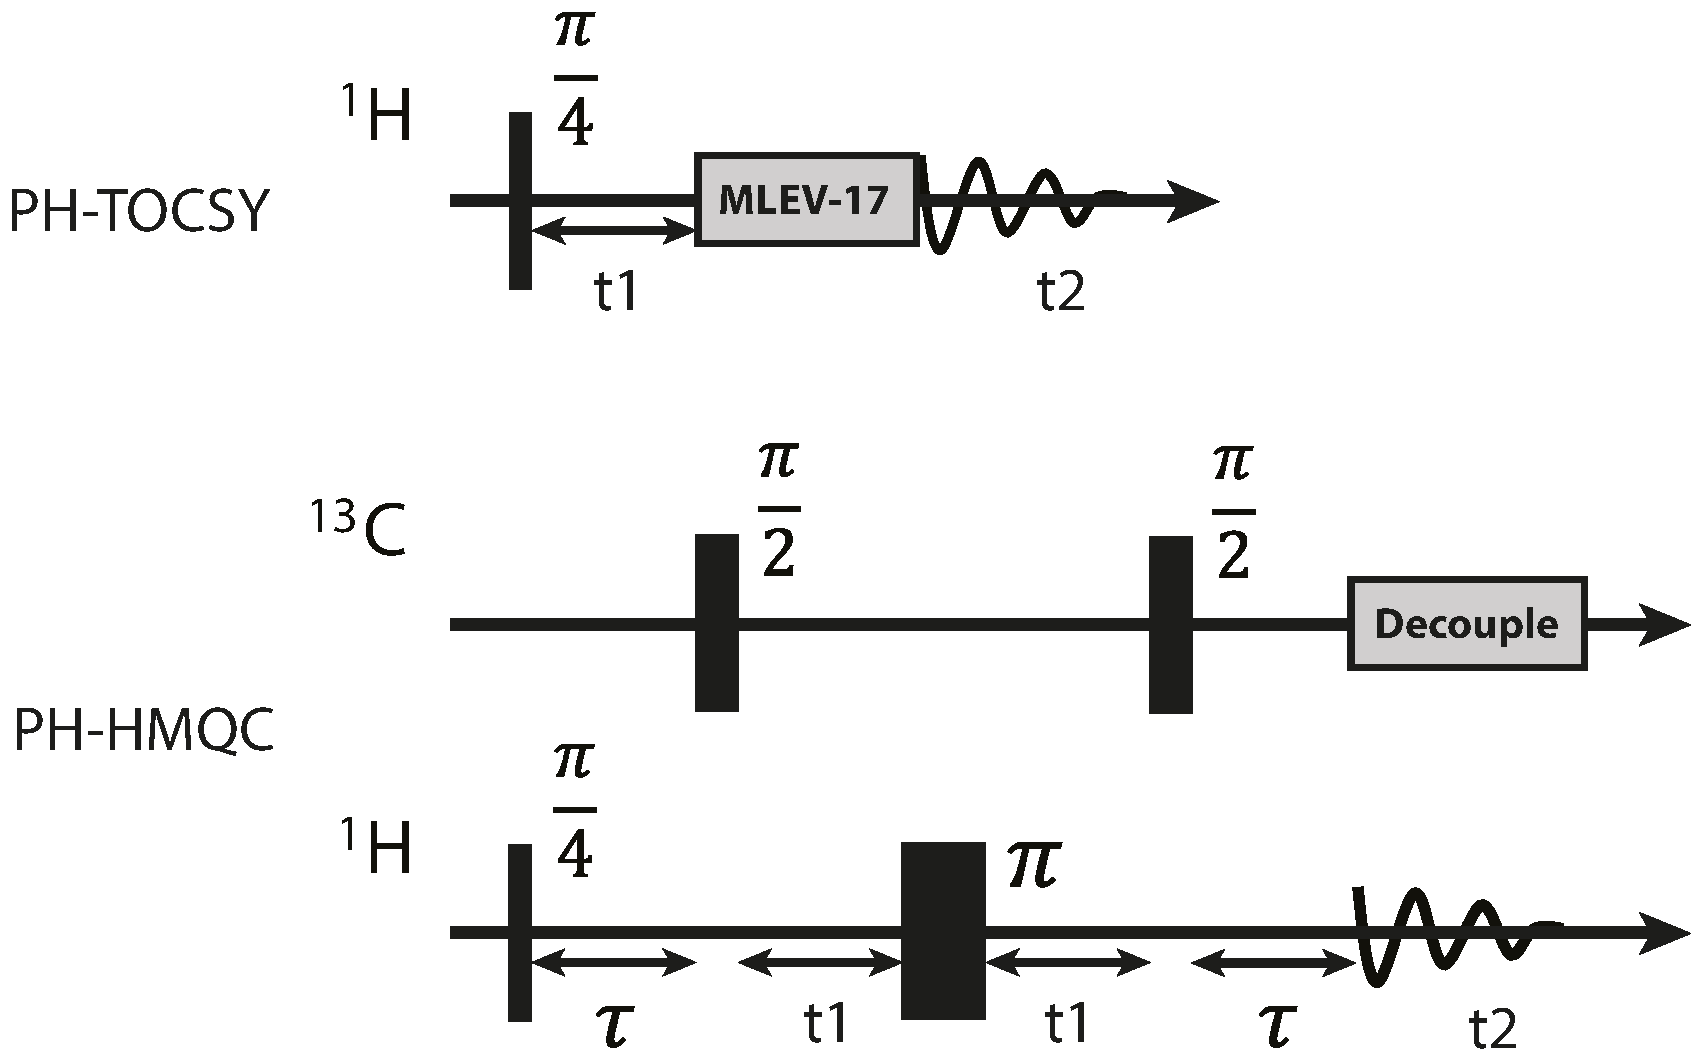
\includegraphics[width=7cm]{PH-TOCSY-HMQC-pulse-sequences.pdf}
\end{center}

\bibliographystyle{rsc}
\bibliography{literature}
\end{document}
%% ----------------------------------------------------------------
